\documentclass[twoside]{book}

% Packages required by doxygen
\usepackage{fixltx2e}
\usepackage{calc}
\usepackage{doxygen}
\usepackage[export]{adjustbox} % also loads graphicx
\usepackage{graphicx}
\usepackage[utf8]{inputenc}
\usepackage{makeidx}
\usepackage{multicol}
\usepackage{multirow}
\PassOptionsToPackage{warn}{textcomp}
\usepackage{textcomp}
\usepackage[nointegrals]{wasysym}
\usepackage[table]{xcolor}

% Font selection
\usepackage[T1]{fontenc}
\usepackage[scaled=.90]{helvet}
\usepackage{courier}
\usepackage{amssymb}
\usepackage{sectsty}
\renewcommand{\familydefault}{\sfdefault}
\allsectionsfont{%
  \fontseries{bc}\selectfont%
  \color{darkgray}%
}
\renewcommand{\DoxyLabelFont}{%
  \fontseries{bc}\selectfont%
  \color{darkgray}%
}
\newcommand{\+}{\discretionary{\mbox{\scriptsize$\hookleftarrow$}}{}{}}

% Page & text layout
\usepackage{geometry}
\geometry{%
  a4paper,%
  top=2.5cm,%
  bottom=2.5cm,%
  left=2.5cm,%
  right=2.5cm%
}
\tolerance=750
\hfuzz=15pt
\hbadness=750
\setlength{\emergencystretch}{15pt}
\setlength{\parindent}{0cm}
\setlength{\parskip}{3ex plus 2ex minus 2ex}
\makeatletter
\renewcommand{\paragraph}{%
  \@startsection{paragraph}{4}{0ex}{-1.0ex}{1.0ex}{%
    \normalfont\normalsize\bfseries\SS@parafont%
  }%
}
\renewcommand{\subparagraph}{%
  \@startsection{subparagraph}{5}{0ex}{-1.0ex}{1.0ex}{%
    \normalfont\normalsize\bfseries\SS@subparafont%
  }%
}
\makeatother

% Headers & footers
\usepackage{fancyhdr}
\pagestyle{fancyplain}
\fancyhead[LE]{\fancyplain{}{\bfseries\thepage}}
\fancyhead[CE]{\fancyplain{}{}}
\fancyhead[RE]{\fancyplain{}{\bfseries\leftmark}}
\fancyhead[LO]{\fancyplain{}{\bfseries\rightmark}}
\fancyhead[CO]{\fancyplain{}{}}
\fancyhead[RO]{\fancyplain{}{\bfseries\thepage}}
\fancyfoot[LE]{\fancyplain{}{}}
\fancyfoot[CE]{\fancyplain{}{}}
\fancyfoot[RE]{\fancyplain{}{\bfseries\scriptsize 構築\+: Doxygen }}
\fancyfoot[LO]{\fancyplain{}{\bfseries\scriptsize 構築\+: Doxygen }}
\fancyfoot[CO]{\fancyplain{}{}}
\fancyfoot[RO]{\fancyplain{}{}}
\renewcommand{\footrulewidth}{0.4pt}
\renewcommand{\chaptermark}[1]{%
  \markboth{#1}{}%
}
\renewcommand{\sectionmark}[1]{%
  \markright{\thesection\ #1}%
}

% Indices & bibliography
\usepackage{natbib}
\usepackage[titles]{tocloft}
\setcounter{tocdepth}{3}
\setcounter{secnumdepth}{5}
\makeindex

% Hyperlinks (required, but should be loaded last)
\usepackage{ifpdf}
\ifpdf
  \usepackage[pdftex,pagebackref=true]{hyperref}
\else
  \usepackage[ps2pdf,pagebackref=true]{hyperref}
\fi
\hypersetup{%
  colorlinks=true,%
  linkcolor=blue,%
  citecolor=blue,%
  unicode%
}

% Custom commands
\newcommand{\clearemptydoublepage}{%
  \newpage{\pagestyle{empty}\cleardoublepage}%
}

\usepackage{caption}
\captionsetup{labelsep=space,justification=centering,font={bf},singlelinecheck=off,skip=4pt,position=top}

%===== C O N T E N T S =====

\begin{document}

% Titlepage & ToC
\hypersetup{pageanchor=false,
             bookmarksnumbered=true,
             pdfencoding=unicode
            }
\pagenumbering{alph}
\begin{titlepage}
\vspace*{7cm}
\begin{center}%
{\Large Saki\+Cpp\+Library }\\
\vspace*{1cm}
{\large 構築\+: Doxygen 1.8.14}\\
\end{center}
\end{titlepage}
\clearemptydoublepage
\pagenumbering{roman}
\tableofcontents
\clearemptydoublepage
\pagenumbering{arabic}
\hypersetup{pageanchor=true}

%--- Begin generated contents ---
\chapter{名前空間索引}
\section{名前空間一覧}
全名前空間の一覧です。\begin{DoxyCompactList}
\item\contentsline{section}{\mbox{\hyperlink{namespacesaki}{saki}} }{\pageref{namespacesaki}}{}
\item\contentsline{section}{\mbox{\hyperlink{namespacesaki_1_1details}{saki\+::details}} }{\pageref{namespacesaki_1_1details}}{}
\end{DoxyCompactList}

\chapter{階層索引}
\section{クラス階層}
クラス階層一覧です。大雑把に文字符号順で並べられています。\begin{DoxyCompactList}
\item \contentsline{section}{saki\+:\+:addition}{\pageref{structsaki_1_1addition}}{}
\item \contentsline{section}{saki\+:\+:array$<$ T, Size $>$}{\pageref{classsaki_1_1array}}{}
\item \contentsline{section}{saki\+:\+:array$<$ saki\+:\+:array$<$ value\+\_\+type, 4 $>$, 4 $>$}{\pageref{classsaki_1_1array}}{}
\item \contentsline{section}{saki\+:\+:array$<$ T, 0 $>$}{\pageref{classsaki_1_1array_3_01_t_00_010_01_4}}{}
\item \contentsline{section}{saki\+:\+:array$<$ T, N $>$}{\pageref{classsaki_1_1array}}{}
\item \contentsline{section}{saki\+:\+:can\+\_\+begin$<$ T $>$}{\pageref{structsaki_1_1can__begin}}{}
\item \contentsline{section}{saki\+:\+:can\+\_\+end$<$ T $>$}{\pageref{structsaki_1_1can__end}}{}
\item \contentsline{section}{saki\+:\+:can\+\_\+range\+\_\+based\+\_\+for$<$ T $>$}{\pageref{classsaki_1_1can__range__based__for}}{}
\item \contentsline{section}{saki\+:\+:clock}{\pageref{classsaki_1_1clock}}{}
\item \contentsline{section}{saki\+:\+:division}{\pageref{structsaki_1_1division}}{}
\item \contentsline{section}{saki\+:\+:enabled\+\_\+if\+\_\+nullptr$<$ bool $>$}{\pageref{structsaki_1_1enabled__if__nullptr}}{}
\item \contentsline{section}{saki\+:\+:enabled\+\_\+if\+\_\+nullptr$<$ true $>$}{\pageref{structsaki_1_1enabled__if__nullptr_3_01true_01_4}}{}
\item \contentsline{section}{saki\+:\+:factorial\+\_\+limits$<$ T $>$}{\pageref{structsaki_1_1factorial__limits}}{}
\item \contentsline{section}{saki\+:\+:factorial\+\_\+limits$<$ char $>$}{\pageref{structsaki_1_1factorial__limits_3_01char_01_4}}{}
\item \contentsline{section}{saki\+:\+:factorial\+\_\+limits$<$ char16\+\_\+t $>$}{\pageref{structsaki_1_1factorial__limits_3_01char16__t_01_4}}{}
\item \contentsline{section}{saki\+:\+:factorial\+\_\+limits$<$ char32\+\_\+t $>$}{\pageref{structsaki_1_1factorial__limits_3_01char32__t_01_4}}{}
\item \contentsline{section}{saki\+:\+:factorial\+\_\+limits$<$ double $>$}{\pageref{structsaki_1_1factorial__limits_3_01double_01_4}}{}
\item \contentsline{section}{saki\+:\+:factorial\+\_\+limits$<$ float $>$}{\pageref{structsaki_1_1factorial__limits_3_01float_01_4}}{}
\item \contentsline{section}{saki\+:\+:factorial\+\_\+limits$<$ int $>$}{\pageref{structsaki_1_1factorial__limits_3_01int_01_4}}{}
\item \contentsline{section}{saki\+:\+:factorial\+\_\+limits$<$ long $>$}{\pageref{structsaki_1_1factorial__limits_3_01long_01_4}}{}
\item \contentsline{section}{saki\+:\+:factorial\+\_\+limits$<$ long double $>$}{\pageref{structsaki_1_1factorial__limits_3_01long_01double_01_4}}{}
\item \contentsline{section}{saki\+:\+:factorial\+\_\+limits$<$ long long $>$}{\pageref{structsaki_1_1factorial__limits_3_01long_01long_01_4}}{}
\item \contentsline{section}{saki\+:\+:factorial\+\_\+limits$<$ short $>$}{\pageref{structsaki_1_1factorial__limits_3_01short_01_4}}{}
\item \contentsline{section}{saki\+:\+:factorial\+\_\+limits$<$ unsigned char $>$}{\pageref{structsaki_1_1factorial__limits_3_01unsigned_01char_01_4}}{}
\item \contentsline{section}{saki\+:\+:factorial\+\_\+limits$<$ unsigned int $>$}{\pageref{structsaki_1_1factorial__limits_3_01unsigned_01int_01_4}}{}
\item \contentsline{section}{saki\+:\+:factorial\+\_\+limits$<$ unsigned long $>$}{\pageref{structsaki_1_1factorial__limits_3_01unsigned_01long_01_4}}{}
\item \contentsline{section}{saki\+:\+:factorial\+\_\+limits$<$ unsigned long long $>$}{\pageref{structsaki_1_1factorial__limits_3_01unsigned_01long_01long_01_4}}{}
\item \contentsline{section}{saki\+:\+:factorial\+\_\+limits$<$ unsigned short $>$}{\pageref{structsaki_1_1factorial__limits_3_01unsigned_01short_01_4}}{}
\item \contentsline{section}{saki\+:\+:factorial\+\_\+limits$<$ wchar\+\_\+t $>$}{\pageref{structsaki_1_1factorial__limits_3_01wchar__t_01_4}}{}
\item \contentsline{section}{saki\+:\+:fibonacci\+\_\+limits$<$ T $>$}{\pageref{structsaki_1_1fibonacci__limits}}{}
\item \contentsline{section}{saki\+:\+:fibonacci\+\_\+limits$<$ char $>$}{\pageref{structsaki_1_1fibonacci__limits_3_01char_01_4}}{}
\item \contentsline{section}{saki\+:\+:fibonacci\+\_\+limits$<$ char16\+\_\+t $>$}{\pageref{structsaki_1_1fibonacci__limits_3_01char16__t_01_4}}{}
\item \contentsline{section}{saki\+:\+:fibonacci\+\_\+limits$<$ char32\+\_\+t $>$}{\pageref{structsaki_1_1fibonacci__limits_3_01char32__t_01_4}}{}
\item \contentsline{section}{saki\+:\+:fibonacci\+\_\+limits$<$ double $>$}{\pageref{structsaki_1_1fibonacci__limits_3_01double_01_4}}{}
\item \contentsline{section}{saki\+:\+:fibonacci\+\_\+limits$<$ float $>$}{\pageref{structsaki_1_1fibonacci__limits_3_01float_01_4}}{}
\item \contentsline{section}{saki\+:\+:fibonacci\+\_\+limits$<$ int $>$}{\pageref{structsaki_1_1fibonacci__limits_3_01int_01_4}}{}
\item \contentsline{section}{saki\+:\+:fibonacci\+\_\+limits$<$ long $>$}{\pageref{structsaki_1_1fibonacci__limits_3_01long_01_4}}{}
\item \contentsline{section}{saki\+:\+:fibonacci\+\_\+limits$<$ long double $>$}{\pageref{structsaki_1_1fibonacci__limits_3_01long_01double_01_4}}{}
\item \contentsline{section}{saki\+:\+:fibonacci\+\_\+limits$<$ long long $>$}{\pageref{structsaki_1_1fibonacci__limits_3_01long_01long_01_4}}{}
\item \contentsline{section}{saki\+:\+:fibonacci\+\_\+limits$<$ short $>$}{\pageref{structsaki_1_1fibonacci__limits_3_01short_01_4}}{}
\item \contentsline{section}{saki\+:\+:fibonacci\+\_\+limits$<$ unsigned char $>$}{\pageref{structsaki_1_1fibonacci__limits_3_01unsigned_01char_01_4}}{}
\item \contentsline{section}{saki\+:\+:fibonacci\+\_\+limits$<$ unsigned int $>$}{\pageref{structsaki_1_1fibonacci__limits_3_01unsigned_01int_01_4}}{}
\item \contentsline{section}{saki\+:\+:fibonacci\+\_\+limits$<$ unsigned long $>$}{\pageref{structsaki_1_1fibonacci__limits_3_01unsigned_01long_01_4}}{}
\item \contentsline{section}{saki\+:\+:fibonacci\+\_\+limits$<$ unsigned long long $>$}{\pageref{structsaki_1_1fibonacci__limits_3_01unsigned_01long_01long_01_4}}{}
\item \contentsline{section}{saki\+:\+:fibonacci\+\_\+limits$<$ unsigned short $>$}{\pageref{structsaki_1_1fibonacci__limits_3_01unsigned_01short_01_4}}{}
\item \contentsline{section}{saki\+:\+:fibonacci\+\_\+limits$<$ wchar\+\_\+t $>$}{\pageref{structsaki_1_1fibonacci__limits_3_01wchar__t_01_4}}{}
\item \contentsline{section}{saki\+:\+:details\+:\+:float\+\_\+constant\+\_\+base$<$ T, Integer, Dec, Zero\+Num $>$}{\pageref{structsaki_1_1details_1_1float__constant__base}}{}
\item \contentsline{section}{saki\+:\+:details\+:\+:float\+\_\+constant\+\_\+base$<$ double, Integer, Dec, Zero\+Num $>$}{\pageref{structsaki_1_1details_1_1float__constant__base}}{}
\begin{DoxyCompactList}
\item \contentsline{section}{saki\+:\+:double\+\_\+constant$<$ Integer, Dec, Zero\+Num $>$}{\pageref{structsaki_1_1double__constant}}{}
\end{DoxyCompactList}
\item \contentsline{section}{saki\+:\+:details\+:\+:float\+\_\+constant\+\_\+base$<$ float, Integer, Dec, Zero\+Num $>$}{\pageref{structsaki_1_1details_1_1float__constant__base}}{}
\begin{DoxyCompactList}
\item \contentsline{section}{saki\+:\+:float\+\_\+constant$<$ Integer, Dec, Zero\+Num $>$}{\pageref{structsaki_1_1float__constant}}{}
\end{DoxyCompactList}
\item \contentsline{section}{saki\+:\+:has\+\_\+check$<$ T $>$}{\pageref{structsaki_1_1has__check}}{}
\item \contentsline{section}{saki\+:\+:has\+\_\+x$<$ T $>$}{\pageref{structsaki_1_1has__x}}{}
\item \contentsline{section}{saki\+:\+:details\+:\+:iterator\+\_\+base$<$ T $>$}{\pageref{classsaki_1_1details_1_1iterator__base}}{}
\begin{DoxyCompactList}
\item \contentsline{section}{saki\+:\+:iterator$<$ T $>$}{\pageref{classsaki_1_1iterator}}{}
\end{DoxyCompactList}
\item \contentsline{section}{saki\+:\+:details\+:\+:iterator\+\_\+base$<$ const T $>$}{\pageref{classsaki_1_1details_1_1iterator__base}}{}
\begin{DoxyCompactList}
\item \contentsline{section}{saki\+:\+:const\+\_\+iterator$<$ T $>$}{\pageref{classsaki_1_1const__iterator}}{}
\end{DoxyCompactList}
\item \contentsline{section}{saki\+:\+:matrix$<$ T $>$}{\pageref{classsaki_1_1matrix}}{}
\item \contentsline{section}{saki\+:\+:Multiple\+Separation}{\pageref{classsaki_1_1_multiple_separation}}{}
\item \contentsline{section}{saki\+:\+:multiplication}{\pageref{structsaki_1_1multiplication}}{}
\item \contentsline{section}{saki\+:\+:Not\+Equal\+Separation}{\pageref{classsaki_1_1_not_equal_separation}}{}
\item \contentsline{section}{saki\+:\+:remove\+\_\+reference\+\_\+const$<$ T $>$}{\pageref{structsaki_1_1remove__reference__const}}{}
\item \contentsline{section}{saki\+:\+:return\+\_\+param}{\pageref{structsaki_1_1return__param}}{}
\item \contentsline{section}{saki\+:\+:details\+:\+:reverse\+\_\+iterator\+\_\+base$<$ T $>$}{\pageref{classsaki_1_1details_1_1reverse__iterator__base}}{}
\begin{DoxyCompactList}
\item \contentsline{section}{saki\+:\+:reverse\+\_\+iterator$<$ T $>$}{\pageref{classsaki_1_1reverse__iterator}}{}
\end{DoxyCompactList}
\item \contentsline{section}{saki\+:\+:details\+:\+:reverse\+\_\+iterator\+\_\+base$<$ const T $>$}{\pageref{classsaki_1_1details_1_1reverse__iterator__base}}{}
\begin{DoxyCompactList}
\item \contentsline{section}{saki\+:\+:const\+\_\+reverse\+\_\+iterator$<$ T $>$}{\pageref{classsaki_1_1const__reverse__iterator}}{}
\end{DoxyCompactList}
\item \contentsline{section}{saki\+:\+:singleton$<$ T $>$}{\pageref{classsaki_1_1singleton}}{}
\item \contentsline{section}{saki\+:\+:string\+\_\+base$<$ T, N $>$}{\pageref{classsaki_1_1string__base}}{}
\item \contentsline{section}{saki\+:\+:subtraction}{\pageref{structsaki_1_1subtraction}}{}
\item \contentsline{section}{saki\+:\+:Transform$<$ T $>$}{\pageref{classsaki_1_1_transform}}{}
\item \contentsline{section}{saki\+:\+:vector2$<$ T $>$}{\pageref{classsaki_1_1vector2}}{}
\item \contentsline{section}{saki\+:\+:vector3$<$ T $>$}{\pageref{classsaki_1_1vector3}}{}
\item \contentsline{section}{saki\+:\+:vector4$<$ T $>$}{\pageref{classsaki_1_1vector4}}{}
\end{DoxyCompactList}

\chapter{クラス索引}
\section{クラス一覧}
クラス・構造体・共用体・インターフェースの一覧です。\begin{DoxyCompactList}
\item\contentsline{section}{\mbox{\hyperlink{structsaki_1_1addition}{saki\+::addition}} \\*足し算のconstexpr対応した関数オブジェクト }{\pageref{structsaki_1_1addition}}{}
\item\contentsline{section}{\mbox{\hyperlink{classsaki_1_1_array}{saki\+::\+Array$<$ T, Size $>$}} \\*コンパイル時固定長配列クラス }{\pageref{classsaki_1_1_array}}{}
\item\contentsline{section}{\mbox{\hyperlink{structsaki_1_1can__begin}{saki\+::can\+\_\+begin$<$ T $>$}} \\*Beginできるかどうかを判定する構造体 }{\pageref{structsaki_1_1can__begin}}{}
\item\contentsline{section}{\mbox{\hyperlink{classsaki_1_1_clock}{saki\+::\+Clock}} \\*時間を測るクラス }{\pageref{classsaki_1_1_clock}}{}
\item\contentsline{section}{\mbox{\hyperlink{structsaki_1_1division}{saki\+::division}} \\*割り算のconstexpr対応した関数オブジェクト }{\pageref{structsaki_1_1division}}{}
\item\contentsline{section}{\mbox{\hyperlink{structsaki_1_1has__check}{saki\+::has\+\_\+check$<$ T $>$}} \\*Check関数を持っているかどうかを判定する構造体 }{\pageref{structsaki_1_1has__check}}{}
\item\contentsline{section}{\mbox{\hyperlink{classsaki_1_1_immobile_ptr}{saki\+::\+Immobile\+Ptr$<$ T $>$}} \\*コピー・ムーブ禁止のスマートポインタ }{\pageref{classsaki_1_1_immobile_ptr}}{}
\item\contentsline{section}{\mbox{\hyperlink{classsaki_1_1_matrix}{saki\+::\+Matrix$<$ T $>$}} \\*行列 }{\pageref{classsaki_1_1_matrix}}{}
\item\contentsline{section}{\mbox{\hyperlink{classsaki_1_1_multiple_separation}{saki\+::\+Multiple\+Separation}} \\*Split関数で利用する、区切り文字を複数指定できるクラス }{\pageref{classsaki_1_1_multiple_separation}}{}
\item\contentsline{section}{\mbox{\hyperlink{structsaki_1_1multiplication}{saki\+::multiplication}} \\*掛け算のconstexpr対応した関数オブジェクト }{\pageref{structsaki_1_1multiplication}}{}
\item\contentsline{section}{\mbox{\hyperlink{classsaki_1_1_node}{saki\+::\+Node$<$ T $>$}} }{\pageref{classsaki_1_1_node}}{}
\item\contentsline{section}{\mbox{\hyperlink{classsaki_1_1_not_equal_separation}{saki\+::\+Not\+Equal\+Separation}} \\*Split関数で利用する、区切らない文字を指定できるクラス }{\pageref{classsaki_1_1_not_equal_separation}}{}
\item\contentsline{section}{\mbox{\hyperlink{structsaki_1_1_return_param}{saki\+::\+Return\+Param}} \\*そのまま引数を返す関数オブジェクト }{\pageref{structsaki_1_1_return_param}}{}
\item\contentsline{section}{\mbox{\hyperlink{classsaki_1_1_singleton}{saki\+::\+Singleton$<$ T $>$}} \\*継承するとシングルトンクラスになる }{\pageref{classsaki_1_1_singleton}}{}
\item\contentsline{section}{\mbox{\hyperlink{structsaki_1_1subtraction}{saki\+::subtraction}} \\*引き算のconstexpr対応した関数オブジェクト }{\pageref{structsaki_1_1subtraction}}{}
\item\contentsline{section}{\mbox{\hyperlink{classsaki_1_1_transform}{saki\+::\+Transform$<$ T $>$}} \\*Transformクラス }{\pageref{classsaki_1_1_transform}}{}
\item\contentsline{section}{\mbox{\hyperlink{classsaki_1_1_tree}{saki\+::\+Tree$<$ T $>$}} }{\pageref{classsaki_1_1_tree}}{}
\item\contentsline{section}{\mbox{\hyperlink{classsaki_1_1_vector2}{saki\+::\+Vector2$<$ T $>$}} \\*2次元でのベクトル }{\pageref{classsaki_1_1_vector2}}{}
\item\contentsline{section}{\mbox{\hyperlink{classsaki_1_1_vector3}{saki\+::\+Vector3$<$ T $>$}} \\*3次元でのベクトル }{\pageref{classsaki_1_1_vector3}}{}
\item\contentsline{section}{\mbox{\hyperlink{classsaki_1_1_vector4}{saki\+::\+Vector4$<$ T $>$}} \\*4次元でのベクトル }{\pageref{classsaki_1_1_vector4}}{}
\end{DoxyCompactList}

\chapter{ファイル索引}
\section{ファイル一覧}
ファイル一覧です。\begin{DoxyCompactList}
\item\contentsline{section}{C\+:/\+Users/tokir/\+Documents/\+Git\+Hub/\+Saki\+Cpp\+Library/saki/\mbox{\hyperlink{min__max_8h}{min\+\_\+max.\+h}} \\*型ごとの最小値と最大値の定数化 }{\pageref{min__max_8h}}{}
\item\contentsline{section}{C\+:/\+Users/tokir/\+Documents/\+Git\+Hub/\+Saki\+Cpp\+Library/saki/\mbox{\hyperlink{pi_8h}{pi.\+h}} \\*円周率のテンプレート変数 }{\pageref{pi_8h}}{}
\item\contentsline{section}{C\+:/\+Users/tokir/\+Documents/\+Git\+Hub/\+Saki\+Cpp\+Library/saki/\mbox{\hyperlink{saki_8h}{saki.\+h}} \\*簡易インクルード(saki) }{\pageref{saki_8h}}{}
\item\contentsline{section}{C\+:/\+Users/tokir/\+Documents/\+Git\+Hub/\+Saki\+Cpp\+Library/saki/\mbox{\hyperlink{type__alias_8h}{type\+\_\+alias.\+h}} \\*型エイリアスを定義 }{\pageref{type__alias_8h}}{}
\item\contentsline{section}{C\+:/\+Users/tokir/\+Documents/\+Git\+Hub/\+Saki\+Cpp\+Library/saki/angle\+\_\+math/\mbox{\hyperlink{angle__math_8h}{angle\+\_\+math.\+h}} \\*簡易インクルード(angle\+\_\+math) }{\pageref{angle__math_8h}}{}
\item\contentsline{section}{C\+:/\+Users/tokir/\+Documents/\+Git\+Hub/\+Saki\+Cpp\+Library/saki/angle\+\_\+math/\mbox{\hyperlink{degree__radian__conversion_8h}{degree\+\_\+radian\+\_\+conversion.\+h}} \\*Degreeから\+Radian、\+Radianから\+Degreeへの変換 }{\pageref{degree__radian__conversion_8h}}{}
\item\contentsline{section}{C\+:/\+Users/tokir/\+Documents/\+Git\+Hub/\+Saki\+Cpp\+Library/saki/constexpr/\mbox{\hyperlink{constexpr_8h}{constexpr.\+h}} \\*簡易インクルード(constexpr) }{\pageref{constexpr_8h}}{}
\item\contentsline{section}{C\+:/\+Users/tokir/\+Documents/\+Git\+Hub/\+Saki\+Cpp\+Library/saki/constexpr/\mbox{\hyperlink{constexpr__abs_8h}{constexpr\+\_\+abs.\+h}} \\*コンパイル時絶対値 }{\pageref{constexpr__abs_8h}}{}
\item\contentsline{section}{C\+:/\+Users/tokir/\+Documents/\+Git\+Hub/\+Saki\+Cpp\+Library/saki/constexpr/\mbox{\hyperlink{constexpr__exchange_8h}{constexpr\+\_\+exchange.\+h}} \\*コンパイル時exchange }{\pageref{constexpr__exchange_8h}}{}
\item\contentsline{section}{C\+:/\+Users/tokir/\+Documents/\+Git\+Hub/\+Saki\+Cpp\+Library/saki/constexpr/\mbox{\hyperlink{constexpr__factorial_8h}{constexpr\+\_\+factorial.\+h}} \\*コンパイル時階乗 }{\pageref{constexpr__factorial_8h}}{}
\item\contentsline{section}{C\+:/\+Users/tokir/\+Documents/\+Git\+Hub/\+Saki\+Cpp\+Library/saki/constexpr/\mbox{\hyperlink{constexpr__sqrt_8h}{constexpr\+\_\+sqrt.\+h}} }{\pageref{constexpr__sqrt_8h}}{}
\item\contentsline{section}{C\+:/\+Users/tokir/\+Documents/\+Git\+Hub/\+Saki\+Cpp\+Library/saki/operator/\mbox{\hyperlink{compare__operator__define_8h}{compare\+\_\+operator\+\_\+define.\+h}} \\*比較系のoperatorを自動で定義するマクロ }{\pageref{compare__operator__define_8h}}{}
\item\contentsline{section}{C\+:/\+Users/tokir/\+Documents/\+Git\+Hub/\+Saki\+Cpp\+Library/saki/operator/\mbox{\hyperlink{compound__assignment__operator__define_8h}{compound\+\_\+assignment\+\_\+operator\+\_\+define.\+h}} \\*複合代入演算子を自動で定義するマクロ }{\pageref{compound__assignment__operator__define_8h}}{}
\item\contentsline{section}{C\+:/\+Users/tokir/\+Documents/\+Git\+Hub/\+Saki\+Cpp\+Library/saki/operator/\mbox{\hyperlink{operator_8h}{operator.\+h}} \\*簡易インクルード(operator) }{\pageref{operator_8h}}{}
\item\contentsline{section}{C\+:/\+Users/tokir/\+Documents/\+Git\+Hub/\+Saki\+Cpp\+Library/saki/random/\mbox{\hyperlink{random_8h}{random.\+h}} \\*決められた範囲でランダムな値を取得する }{\pageref{random_8h}}{}
\item\contentsline{section}{C\+:/\+Users/tokir/\+Documents/\+Git\+Hub/\+Saki\+Cpp\+Library/saki/simplified-\/method/\mbox{\hyperlink{simplified__method_8h}{simplified\+\_\+method.\+h}} \\*簡易インクルード(simplified\+\_\+method) }{\pageref{simplified__method_8h}}{}
\item\contentsline{section}{C\+:/\+Users/tokir/\+Documents/\+Git\+Hub/\+Saki\+Cpp\+Library/saki/simplified-\/method/accumulate/\mbox{\hyperlink{accumulate_8h}{accumulate.\+h}} \\*既存のaccumulate関数の簡略化 }{\pageref{accumulate_8h}}{}
\item\contentsline{section}{C\+:/\+Users/tokir/\+Documents/\+Git\+Hub/\+Saki\+Cpp\+Library/saki/simplified-\/method/for\+\_\+each/\mbox{\hyperlink{for__each_8h}{for\+\_\+each.\+h}} \\*既存のfor\+\_\+each関数の簡略化+拡張 }{\pageref{for__each_8h}}{}
\item\contentsline{section}{C\+:/\+Users/tokir/\+Documents/\+Git\+Hub/\+Saki\+Cpp\+Library/saki/simplified-\/method/iota/\mbox{\hyperlink{iota_8h}{iota.\+h}} \\*既存のiota関数の簡略化+拡張 }{\pageref{iota_8h}}{}
\item\contentsline{section}{C\+:/\+Users/tokir/\+Documents/\+Git\+Hub/\+Saki\+Cpp\+Library/saki/singleton/\mbox{\hyperlink{singleton_8h}{singleton.\+h}} \\*シングルトンクラス }{\pageref{singleton_8h}}{}
\item\contentsline{section}{C\+:/\+Users/tokir/\+Documents/\+Git\+Hub/\+Saki\+Cpp\+Library/saki/smart\+\_\+ptr/\mbox{\hyperlink{smart__ptr_8h}{smart\+\_\+ptr.\+h}} \\*簡易インクルード(smart\+\_\+ptr) }{\pageref{smart__ptr_8h}}{}
\item\contentsline{section}{C\+:/\+Users/tokir/\+Documents/\+Git\+Hub/\+Saki\+Cpp\+Library/saki/smart\+\_\+ptr/immobile/\mbox{\hyperlink{immobile__ptr_8h}{immobile\+\_\+ptr.\+h}} \\*コピー・ムーブ禁止のスマートポインタ }{\pageref{immobile__ptr_8h}}{}
\item\contentsline{section}{C\+:/\+Users/tokir/\+Documents/\+Git\+Hub/\+Saki\+Cpp\+Library/saki/vector/\mbox{\hyperlink{vector_8h}{vector.\+h}} \\*簡易インクルード(vector) }{\pageref{vector_8h}}{}
\item\contentsline{section}{C\+:/\+Users/tokir/\+Documents/\+Git\+Hub/\+Saki\+Cpp\+Library/saki/vector/\mbox{\hyperlink{vector__2d_8h}{vector\+\_\+2d.\+h}} \\*2次元でのベクトル }{\pageref{vector__2d_8h}}{}
\item\contentsline{section}{C\+:/\+Users/tokir/\+Documents/\+Git\+Hub/\+Saki\+Cpp\+Library/saki/vector/\mbox{\hyperlink{vector__3d_8h}{vector\+\_\+3d.\+h}} \\*3次元でのベクトル }{\pageref{vector__3d_8h}}{}
\end{DoxyCompactList}

\chapter{名前空間詳解}
\hypertarget{namespacesaki}{}\section{saki 名前空間}
\label{namespacesaki}\index{saki@{saki}}
\subsection*{名前空間}
\begin{DoxyCompactItemize}
\item 
 \mbox{\hyperlink{namespacesaki_1_1details}{details}}
\item 
 \mbox{\hyperlink{namespacesaki_1_1impl}{impl}}
\end{DoxyCompactItemize}
\subsection*{クラス}
\begin{DoxyCompactItemize}
\item 
struct \mbox{\hyperlink{structsaki_1_1addition}{addition}}
\begin{DoxyCompactList}\small\item\em 足し算のconstexpr対応した関数オブジェクト \end{DoxyCompactList}\item 
class \mbox{\hyperlink{classsaki_1_1array}{array}}
\begin{DoxyCompactList}\small\item\em コンパイル時固定長配列クラス \end{DoxyCompactList}\item 
class \mbox{\hyperlink{classsaki_1_1array_3_01_t_00_010_01_4}{array$<$ T, 0 $>$}}
\item 
struct \mbox{\hyperlink{structsaki_1_1can__begin}{can\+\_\+begin}}
\begin{DoxyCompactList}\small\item\em beginできるかどうかを判定する構造体 \end{DoxyCompactList}\item 
struct \mbox{\hyperlink{structsaki_1_1can__different__equal}{can\+\_\+different\+\_\+equal}}
\begin{DoxyCompactList}\small\item\em 代入演算子を定義しているかどうかを判定する構造体(違う型同士) \end{DoxyCompactList}\item 
struct \mbox{\hyperlink{structsaki_1_1can__different__equal_3_01_t_00_01_t_01_4}{can\+\_\+different\+\_\+equal$<$ T, T $>$}}
\item 
struct \mbox{\hyperlink{structsaki_1_1can__end}{can\+\_\+end}}
\begin{DoxyCompactList}\small\item\em endできるかどうかを判定する構造体 \end{DoxyCompactList}\item 
struct \mbox{\hyperlink{structsaki_1_1can__equal__equal}{can\+\_\+equal\+\_\+equal}}
\begin{DoxyCompactList}\small\item\em イコールイコール比較できるかどうかを判定する構造体(==) \end{DoxyCompactList}\item 
struct \mbox{\hyperlink{structsaki_1_1can__greater}{can\+\_\+greater}}
\begin{DoxyCompactList}\small\item\em より大きい比較できるかどうかを判定する構造体($>$) \end{DoxyCompactList}\item 
struct \mbox{\hyperlink{structsaki_1_1can__greater__or__equal}{can\+\_\+greater\+\_\+or\+\_\+equal}}
\begin{DoxyCompactList}\small\item\em 以上比較できるかどうかを判定する構造体($>$=) \end{DoxyCompactList}\item 
struct \mbox{\hyperlink{structsaki_1_1can__less}{can\+\_\+less}}
\begin{DoxyCompactList}\small\item\em より小さい比較できるかどうかを判定する構造体($<$) \end{DoxyCompactList}\item 
struct \mbox{\hyperlink{structsaki_1_1can__less__or__equal}{can\+\_\+less\+\_\+or\+\_\+equal}}
\begin{DoxyCompactList}\small\item\em 以下比較できるかどうかを判定する構造体($<$=) \end{DoxyCompactList}\item 
struct \mbox{\hyperlink{structsaki_1_1can__not__equal}{can\+\_\+not\+\_\+equal}}
\begin{DoxyCompactList}\small\item\em ノットイコール比較できるかどうかを判定する構造体(!=) \end{DoxyCompactList}\item 
struct \mbox{\hyperlink{structsaki_1_1can__ostream}{can\+\_\+ostream}}
\begin{DoxyCompactList}\small\item\em ostream演算子をオーバーロードしているかどうか判定する構造体(cout) \end{DoxyCompactList}\item 
class \mbox{\hyperlink{classsaki_1_1can__range__based__for}{can\+\_\+range\+\_\+based\+\_\+for}}
\begin{DoxyCompactList}\small\item\em 範囲ベースfor文に利用できる型かどうか判定する \end{DoxyCompactList}\item 
struct \mbox{\hyperlink{structsaki_1_1can__same__equal}{can\+\_\+same\+\_\+equal}}
\begin{DoxyCompactList}\small\item\em 代入演算子を定義しているかどうかを判定する構造体(同じ型同士) \end{DoxyCompactList}\item 
class \mbox{\hyperlink{classsaki_1_1clock}{clock}}
\begin{DoxyCompactList}\small\item\em 時間を測るクラス \end{DoxyCompactList}\item 
class \mbox{\hyperlink{classsaki_1_1const__iterator}{const\+\_\+iterator}}
\begin{DoxyCompactList}\small\item\em constなイテレーター \end{DoxyCompactList}\item 
class \mbox{\hyperlink{classsaki_1_1const__reverse__iterator}{const\+\_\+reverse\+\_\+iterator}}
\begin{DoxyCompactList}\small\item\em constなリバースイテレーター \end{DoxyCompactList}\item 
struct \mbox{\hyperlink{structsaki_1_1division}{division}}
\begin{DoxyCompactList}\small\item\em 割り算のconstexpr対応した関数オブジェクト \end{DoxyCompactList}\item 
struct \mbox{\hyperlink{structsaki_1_1double__constant}{double\+\_\+constant}}
\begin{DoxyCompactList}\small\item\em 倍精度浮動小数点型の定数を表す \end{DoxyCompactList}\item 
struct \mbox{\hyperlink{structsaki_1_1enable__if__nullptr}{enable\+\_\+if\+\_\+nullptr}}
\begin{DoxyCompactList}\small\item\em enalbe\+\_\+ifのfalse \end{DoxyCompactList}\item 
struct \mbox{\hyperlink{structsaki_1_1enable__if__nullptr_3_01true_01_4}{enable\+\_\+if\+\_\+nullptr$<$ true $>$}}
\begin{DoxyCompactList}\small\item\em enable\+\_\+ifのtrue \end{DoxyCompactList}\item 
struct \mbox{\hyperlink{structsaki_1_1factorial__limits}{factorial\+\_\+limits}}
\begin{DoxyCompactList}\small\item\em 型ごとの最大階乗数 \end{DoxyCompactList}\item 
struct \mbox{\hyperlink{structsaki_1_1factorial__limits_3_01char_01_4}{factorial\+\_\+limits$<$ char $>$}}
\item 
struct \mbox{\hyperlink{structsaki_1_1factorial__limits_3_01char16__t_01_4}{factorial\+\_\+limits$<$ char16\+\_\+t $>$}}
\item 
struct \mbox{\hyperlink{structsaki_1_1factorial__limits_3_01char32__t_01_4}{factorial\+\_\+limits$<$ char32\+\_\+t $>$}}
\item 
struct \mbox{\hyperlink{structsaki_1_1factorial__limits_3_01double_01_4}{factorial\+\_\+limits$<$ double $>$}}
\item 
struct \mbox{\hyperlink{structsaki_1_1factorial__limits_3_01float_01_4}{factorial\+\_\+limits$<$ float $>$}}
\item 
struct \mbox{\hyperlink{structsaki_1_1factorial__limits_3_01int_01_4}{factorial\+\_\+limits$<$ int $>$}}
\item 
struct \mbox{\hyperlink{structsaki_1_1factorial__limits_3_01long_01_4}{factorial\+\_\+limits$<$ long $>$}}
\item 
struct \mbox{\hyperlink{structsaki_1_1factorial__limits_3_01long_01double_01_4}{factorial\+\_\+limits$<$ long double $>$}}
\item 
struct \mbox{\hyperlink{structsaki_1_1factorial__limits_3_01long_01long_01_4}{factorial\+\_\+limits$<$ long long $>$}}
\item 
struct \mbox{\hyperlink{structsaki_1_1factorial__limits_3_01short_01_4}{factorial\+\_\+limits$<$ short $>$}}
\item 
struct \mbox{\hyperlink{structsaki_1_1factorial__limits_3_01unsigned_01char_01_4}{factorial\+\_\+limits$<$ unsigned char $>$}}
\item 
struct \mbox{\hyperlink{structsaki_1_1factorial__limits_3_01unsigned_01int_01_4}{factorial\+\_\+limits$<$ unsigned int $>$}}
\item 
struct \mbox{\hyperlink{structsaki_1_1factorial__limits_3_01unsigned_01long_01_4}{factorial\+\_\+limits$<$ unsigned long $>$}}
\item 
struct \mbox{\hyperlink{structsaki_1_1factorial__limits_3_01unsigned_01long_01long_01_4}{factorial\+\_\+limits$<$ unsigned long long $>$}}
\item 
struct \mbox{\hyperlink{structsaki_1_1factorial__limits_3_01unsigned_01short_01_4}{factorial\+\_\+limits$<$ unsigned short $>$}}
\item 
struct \mbox{\hyperlink{structsaki_1_1factorial__limits_3_01wchar__t_01_4}{factorial\+\_\+limits$<$ wchar\+\_\+t $>$}}
\item 
struct \mbox{\hyperlink{structsaki_1_1fibonacci__limits}{fibonacci\+\_\+limits}}
\begin{DoxyCompactList}\small\item\em 型ごとのフィボナッチ数 \end{DoxyCompactList}\item 
struct \mbox{\hyperlink{structsaki_1_1fibonacci__limits_3_01char_01_4}{fibonacci\+\_\+limits$<$ char $>$}}
\item 
struct \mbox{\hyperlink{structsaki_1_1fibonacci__limits_3_01char16__t_01_4}{fibonacci\+\_\+limits$<$ char16\+\_\+t $>$}}
\item 
struct \mbox{\hyperlink{structsaki_1_1fibonacci__limits_3_01char32__t_01_4}{fibonacci\+\_\+limits$<$ char32\+\_\+t $>$}}
\item 
struct \mbox{\hyperlink{structsaki_1_1fibonacci__limits_3_01double_01_4}{fibonacci\+\_\+limits$<$ double $>$}}
\item 
struct \mbox{\hyperlink{structsaki_1_1fibonacci__limits_3_01float_01_4}{fibonacci\+\_\+limits$<$ float $>$}}
\item 
struct \mbox{\hyperlink{structsaki_1_1fibonacci__limits_3_01int_01_4}{fibonacci\+\_\+limits$<$ int $>$}}
\item 
struct \mbox{\hyperlink{structsaki_1_1fibonacci__limits_3_01long_01_4}{fibonacci\+\_\+limits$<$ long $>$}}
\item 
struct \mbox{\hyperlink{structsaki_1_1fibonacci__limits_3_01long_01double_01_4}{fibonacci\+\_\+limits$<$ long double $>$}}
\item 
struct \mbox{\hyperlink{structsaki_1_1fibonacci__limits_3_01long_01long_01_4}{fibonacci\+\_\+limits$<$ long long $>$}}
\item 
struct \mbox{\hyperlink{structsaki_1_1fibonacci__limits_3_01short_01_4}{fibonacci\+\_\+limits$<$ short $>$}}
\item 
struct \mbox{\hyperlink{structsaki_1_1fibonacci__limits_3_01unsigned_01char_01_4}{fibonacci\+\_\+limits$<$ unsigned char $>$}}
\item 
struct \mbox{\hyperlink{structsaki_1_1fibonacci__limits_3_01unsigned_01int_01_4}{fibonacci\+\_\+limits$<$ unsigned int $>$}}
\item 
struct \mbox{\hyperlink{structsaki_1_1fibonacci__limits_3_01unsigned_01long_01_4}{fibonacci\+\_\+limits$<$ unsigned long $>$}}
\item 
struct \mbox{\hyperlink{structsaki_1_1fibonacci__limits_3_01unsigned_01long_01long_01_4}{fibonacci\+\_\+limits$<$ unsigned long long $>$}}
\item 
struct \mbox{\hyperlink{structsaki_1_1fibonacci__limits_3_01unsigned_01short_01_4}{fibonacci\+\_\+limits$<$ unsigned short $>$}}
\item 
struct \mbox{\hyperlink{structsaki_1_1fibonacci__limits_3_01wchar__t_01_4}{fibonacci\+\_\+limits$<$ wchar\+\_\+t $>$}}
\item 
struct \mbox{\hyperlink{structsaki_1_1float__constant}{float\+\_\+constant}}
\begin{DoxyCompactList}\small\item\em 浮動小数点型の定数を表す \end{DoxyCompactList}\item 
struct \mbox{\hyperlink{structsaki_1_1has__check}{has\+\_\+check}}
\begin{DoxyCompactList}\small\item\em check関数を持っているかどうかを判定する構造体 \end{DoxyCompactList}\item 
struct \mbox{\hyperlink{structsaki_1_1has__x}{has\+\_\+x}}
\begin{DoxyCompactList}\small\item\em 変数xを持っているかどうかを判定する構造体 \end{DoxyCompactList}\item 
struct \mbox{\hyperlink{structsaki_1_1has__y}{has\+\_\+y}}
\begin{DoxyCompactList}\small\item\em 変数yを持っているかどうかを判定する構造体 \end{DoxyCompactList}\item 
struct \mbox{\hyperlink{structsaki_1_1has__z}{has\+\_\+z}}
\begin{DoxyCompactList}\small\item\em 変数yを持っているかどうかを判定する構造体 \end{DoxyCompactList}\item 
class \mbox{\hyperlink{classsaki_1_1iterator}{iterator}}
\begin{DoxyCompactList}\small\item\em ノーマルなイテレーター \end{DoxyCompactList}\item 
class \mbox{\hyperlink{classsaki_1_1matrix}{matrix}}
\begin{DoxyCompactList}\small\item\em 行列 \end{DoxyCompactList}\item 
class \mbox{\hyperlink{classsaki_1_1_multiple_separation}{Multiple\+Separation}}
\begin{DoxyCompactList}\small\item\em split関数で利用する、区切り文字を複数指定できるクラス \end{DoxyCompactList}\item 
struct \mbox{\hyperlink{structsaki_1_1multiplication}{multiplication}}
\begin{DoxyCompactList}\small\item\em 掛け算のconstexpr対応した関数オブジェクト \end{DoxyCompactList}\item 
class \mbox{\hyperlink{classsaki_1_1_not_equal_separation}{Not\+Equal\+Separation}}
\begin{DoxyCompactList}\small\item\em split関数で利用する、区切らない文字を指定できるクラス \end{DoxyCompactList}\item 
struct \mbox{\hyperlink{structsaki_1_1remove__reference__const}{remove\+\_\+reference\+\_\+const}}
\begin{DoxyCompactList}\small\item\em 参照とconst修飾を削除 \end{DoxyCompactList}\item 
struct \mbox{\hyperlink{structsaki_1_1return__param}{return\+\_\+param}}
\begin{DoxyCompactList}\small\item\em そのまま引数を返す関数オブジェクト \end{DoxyCompactList}\item 
class \mbox{\hyperlink{classsaki_1_1reverse__iterator}{reverse\+\_\+iterator}}
\begin{DoxyCompactList}\small\item\em ノーマルなリバースイテレーター \end{DoxyCompactList}\item 
class \mbox{\hyperlink{classsaki_1_1singleton}{singleton}}
\begin{DoxyCompactList}\small\item\em 継承するとシングルトンクラスになる \end{DoxyCompactList}\item 
class \mbox{\hyperlink{classsaki_1_1string__base}{string\+\_\+base}}
\begin{DoxyCompactList}\small\item\em コンパイル時固定長string\+\_\+baseクラス \end{DoxyCompactList}\item 
struct \mbox{\hyperlink{structsaki_1_1subtraction}{subtraction}}
\begin{DoxyCompactList}\small\item\em 引き算のconstexpr対応した関数オブジェクト \end{DoxyCompactList}\item 
class \mbox{\hyperlink{classsaki_1_1transform}{transform}}
\begin{DoxyCompactList}\small\item\em transformクラス \end{DoxyCompactList}\item 
class \mbox{\hyperlink{classsaki_1_1vector2}{vector2}}
\begin{DoxyCompactList}\small\item\em 2次元でのベクトル \end{DoxyCompactList}\item 
class \mbox{\hyperlink{classsaki_1_1vector3}{vector3}}
\begin{DoxyCompactList}\small\item\em 3次元でのベクトル \end{DoxyCompactList}\item 
class \mbox{\hyperlink{classsaki_1_1vector4}{vector4}}
\begin{DoxyCompactList}\small\item\em 4次元でのベクトル \end{DoxyCompactList}\end{DoxyCompactItemize}
\subsection*{型定義}
\begin{DoxyCompactItemize}
\item 
{\footnotesize template$<$size\+\_\+t N$>$ }\\using \mbox{\hyperlink{namespacesaki_a47847d63f1d9c97ca37f33eeecb27674}{string}} = \mbox{\hyperlink{classsaki_1_1string__base}{saki\+::string\+\_\+base}}$<$ char, N $>$
\item 
{\footnotesize template$<$bool Con$>$ }\\using \mbox{\hyperlink{namespacesaki_a4c362f5119aac94085eab0bf794facf7}{enable\+\_\+if\+\_\+nullptr\+\_\+t}} = typename \mbox{\hyperlink{structsaki_1_1enable__if__nullptr}{enable\+\_\+if\+\_\+nullptr}}$<$ Con $>$\+::type
\begin{DoxyCompactList}\small\item\em enable\+\_\+if\+\_\+nullptrを簡単に呼び出せる変数 \end{DoxyCompactList}\item 
{\footnotesize template$<$typename T $>$ }\\using \mbox{\hyperlink{namespacesaki_aff6964622fdfcdf489dab4b87727a8e4}{remove\+\_\+reference\+\_\+const\+\_\+t}} = typename \mbox{\hyperlink{structsaki_1_1remove__reference__const}{saki\+::remove\+\_\+reference\+\_\+const}}$<$ T $>$\+::type
\begin{DoxyCompactList}\small\item\em remove\+\_\+reference\+\_\+constを簡単に呼び出せるようにした \end{DoxyCompactList}\end{DoxyCompactItemize}
\subsection*{関数}
\begin{DoxyCompactItemize}
\item 
{\footnotesize template$<$typename Container1 , typename Container2 , saki\+::enable\+\_\+if\+\_\+nullptr\+\_\+t$<$ saki\+::can\+\_\+range\+\_\+based\+\_\+for\+\_\+v$<$ Container1 $>$ \&\&saki\+::can\+\_\+range\+\_\+based\+\_\+for\+\_\+v$<$ Container2 $>$ $>$  = nullptr$>$ }\\constexpr auto \mbox{\hyperlink{namespacesaki_abd8c75003f2a213607842f5d82eac806}{copy}} (const Container1 \&con1, Container2 \&con2) -\/$>$ decltype($\ast$std\+::begin(con2)= $\ast$std\+::begin(con1), std\+::begin(con2))
\begin{DoxyCompactList}\small\item\em コンテナとコンテナを渡すcopy \end{DoxyCompactList}\item 
{\footnotesize template$<$typename T , size\+\_\+t Size$>$ }\\constexpr bool \mbox{\hyperlink{namespacesaki_a5ce8a66ed6ece15fa9ddeaec2746374d}{operator==}} (const \mbox{\hyperlink{classsaki_1_1array}{array}}$<$ T, Size $>$ \&arr1, const \mbox{\hyperlink{classsaki_1_1array}{array}}$<$ T, Size $>$ \&arr2)
\begin{DoxyCompactList}\small\item\em ==演算子 \end{DoxyCompactList}\item 
{\footnotesize template$<$typename T , size\+\_\+t Size$>$ }\\constexpr bool \mbox{\hyperlink{namespacesaki_aed742cc915a830fea9f4993c0a031c45}{operator!=}} (const \mbox{\hyperlink{classsaki_1_1array}{array}}$<$ T, Size $>$ \&arr1, const \mbox{\hyperlink{classsaki_1_1array}{array}}$<$ T, Size $>$ \&arr2)
\begin{DoxyCompactList}\small\item\em !=演算子 \end{DoxyCompactList}\item 
{\footnotesize template$<$typename T , saki\+::enable\+\_\+if\+\_\+nullptr\+\_\+t$<$ saki\+::can\+\_\+less\+\_\+or\+\_\+equal\+\_\+v$<$ T $>$ $>$  = nullptr$>$ }\\constexpr bool \mbox{\hyperlink{namespacesaki_a45597d7382905409bada2316f78502fc}{is\+\_\+fit}} (const T \&x, const T \&min\+\_\+n, const T \&max\+\_\+n)
\begin{DoxyCompactList}\small\item\em 範囲内かどうかの判定を行う \end{DoxyCompactList}\item 
{\footnotesize template$<$typename First , typename Min\+Type , typename Max\+Type , saki\+::enable\+\_\+if\+\_\+nullptr\+\_\+t$<$ std\+::is\+\_\+convertible\+\_\+v$<$ Min\+Type, First $>$ \&\&std\+::is\+\_\+convertible\+\_\+v$<$ Max\+Type, First $>$ \&\&saki\+::can\+\_\+less\+\_\+or\+\_\+equal\+\_\+v$<$ First $>$ $>$  = nullptr$>$ }\\constexpr bool \mbox{\hyperlink{namespacesaki_a09478d8cb01d75e93d34f884d7133dc9}{is\+\_\+fit}} (First x, Min\+Type min\+\_\+n, Max\+Type max\+\_\+n)
\begin{DoxyCompactList}\small\item\em 型をそろえる \end{DoxyCompactList}\item 
{\footnotesize template$<$typename First , typename... Args, saki\+::enable\+\_\+if\+\_\+nullptr\+\_\+t$<$ std\+::conjunction\+\_\+v$<$ std\+::is\+\_\+convertible$<$ Args, First $>$... $>$ \&\&std\+::conjunction\+\_\+v$<$ saki\+::can\+\_\+less$<$ First $>$$>$ $>$  = nullptr$>$ }\\constexpr bool \mbox{\hyperlink{namespacesaki_af73b5897b021844313675413b6c8aac2}{is\+\_\+max}} (const First \&first, const Args \&... args)
\begin{DoxyCompactList}\small\item\em 複数の比較を一度に行える($>$=) \end{DoxyCompactList}\item 
{\footnotesize template$<$typename First , typename... Args, saki\+::enable\+\_\+if\+\_\+nullptr\+\_\+t$<$ std\+::conjunction\+\_\+v$<$ std\+::is\+\_\+convertible$<$ First, Args $>$... $>$ \&\&std\+::conjunction\+\_\+v$<$ saki\+::can\+\_\+greater$<$ First $>$$>$ $>$  = nullptr$>$ }\\constexpr bool \mbox{\hyperlink{namespacesaki_a761604ec865e518ea0ba335b709be060}{is\+\_\+min}} (const First \&first, const Args \&... args)
\begin{DoxyCompactList}\small\item\em 複数の比較を一度に行える($<$=) \end{DoxyCompactList}\item 
{\footnotesize template$<$typename First , typename... Args, saki\+::enable\+\_\+if\+\_\+nullptr\+\_\+t$<$ std\+::conjunction\+\_\+v$<$ std\+::is\+\_\+convertible$<$ First, Args $>$... $>$ \&\&std\+::conjunction\+\_\+v$<$ saki\+::can\+\_\+equal\+\_\+equal$<$ First $>$$>$ $>$  = nullptr$>$ }\\constexpr bool \mbox{\hyperlink{namespacesaki_a098cd355949dd93ffdaf620f0fc7e236}{multi\+\_\+equal}} (const First \&first, const Args \&... args)
\begin{DoxyCompactList}\small\item\em 複数の比較を一度に行える \end{DoxyCompactList}\item 
{\footnotesize template$<$typename T , saki\+::enable\+\_\+if\+\_\+nullptr\+\_\+t$<$!std\+::is\+\_\+unsigned\+\_\+v$<$ T $>$$>$  = nullptr$>$ }\\constexpr T \mbox{\hyperlink{namespacesaki_a37cd607ad87b208aa6105b5d8287dc9e}{abs}} (T x)
\begin{DoxyCompactList}\small\item\em コンパイル時絶対値 \end{DoxyCompactList}\item 
{\footnotesize template$<$typename T , saki\+::enable\+\_\+if\+\_\+nullptr\+\_\+t$<$ std\+::is\+\_\+floating\+\_\+point\+\_\+v$<$ T $>$$>$  = nullptr$>$ }\\constexpr T \mbox{\hyperlink{namespacesaki_a3189b75c5c7ecbf6d2204142da5fa813}{acos}} (T x)
\begin{DoxyCompactList}\small\item\em コンパイル時acos \end{DoxyCompactList}\item 
{\footnotesize template$<$typename T , saki\+::enable\+\_\+if\+\_\+nullptr\+\_\+t$<$ std\+::is\+\_\+integral\+\_\+v$<$ T $>$$>$  = nullptr$>$ }\\constexpr double \mbox{\hyperlink{namespacesaki_a2cad65bf92f361b4b564268af96a7844}{acos}} (T x)
\begin{DoxyCompactList}\small\item\em 引数がint型の場合に、戻り値をdouble型にするためのもの \end{DoxyCompactList}\item 
{\footnotesize template$<$typename T , saki\+::enable\+\_\+if\+\_\+nullptr\+\_\+t$<$ std\+::is\+\_\+floating\+\_\+point\+\_\+v$<$ T $>$$>$  = nullptr$>$ }\\constexpr T \mbox{\hyperlink{namespacesaki_ac1c85a4defc25dc9eb6b380f29946f83}{acosh}} (T x)
\begin{DoxyCompactList}\small\item\em コンパイル時sinh \end{DoxyCompactList}\item 
{\footnotesize template$<$typename T , saki\+::enable\+\_\+if\+\_\+nullptr\+\_\+t$<$ std\+::is\+\_\+integral\+\_\+v$<$ T $>$$>$  = nullptr$>$ }\\constexpr double \mbox{\hyperlink{namespacesaki_a8d3766d425082661e966b04504b90002}{acosh}} (T x)
\begin{DoxyCompactList}\small\item\em 引数がint型の場合に、戻り値をdouble型にするためのもの \end{DoxyCompactList}\item 
{\footnotesize template$<$typename T , saki\+::enable\+\_\+if\+\_\+nullptr\+\_\+t$<$ std\+::is\+\_\+floating\+\_\+point\+\_\+v$<$ T $>$$>$  = nullptr$>$ }\\constexpr T \mbox{\hyperlink{namespacesaki_a63f2b40515cd62b037dade64aa8465db}{asin}} (T x)
\begin{DoxyCompactList}\small\item\em コンパイル時asin \end{DoxyCompactList}\item 
{\footnotesize template$<$typename T , saki\+::enable\+\_\+if\+\_\+nullptr\+\_\+t$<$ std\+::is\+\_\+integral\+\_\+v$<$ T $>$$>$  = nullptr$>$ }\\constexpr double \mbox{\hyperlink{namespacesaki_aac285debedd1f53761a838c0e4f57af0}{asin}} (T x)
\begin{DoxyCompactList}\small\item\em 引数がint型の場合に、戻り値をdouble型にするためのもの \end{DoxyCompactList}\item 
{\footnotesize template$<$typename T , saki\+::enable\+\_\+if\+\_\+nullptr\+\_\+t$<$ std\+::is\+\_\+floating\+\_\+point\+\_\+v$<$ T $>$$>$  = nullptr$>$ }\\constexpr T \mbox{\hyperlink{namespacesaki_ab097a2d600f313b6bdd3099e61a10b9e}{asinh}} (T x)
\begin{DoxyCompactList}\small\item\em コンパイル時asinh \end{DoxyCompactList}\item 
{\footnotesize template$<$typename T , saki\+::enable\+\_\+if\+\_\+nullptr\+\_\+t$<$ std\+::is\+\_\+integral\+\_\+v$<$ T $>$$>$  = nullptr$>$ }\\constexpr double \mbox{\hyperlink{namespacesaki_aac840ca5d9b98ac0a8c5b15752f02072}{asinh}} (T x)
\begin{DoxyCompactList}\small\item\em 引数がint型の場合に、戻り値をdouble型にするためのもの \end{DoxyCompactList}\item 
{\footnotesize template$<$typename T , saki\+::enable\+\_\+if\+\_\+nullptr\+\_\+t$<$ std\+::is\+\_\+floating\+\_\+point\+\_\+v$<$ T $>$$>$  = nullptr$>$ }\\constexpr T \mbox{\hyperlink{namespacesaki_a524b9439c745f69bd8a8b681b03b4b01}{atan}} (T x)
\begin{DoxyCompactList}\small\item\em コンパイル時atan \end{DoxyCompactList}\item 
{\footnotesize template$<$typename T , saki\+::enable\+\_\+if\+\_\+nullptr\+\_\+t$<$ std\+::is\+\_\+integral\+\_\+v$<$ T $>$$>$  = nullptr$>$ }\\constexpr double \mbox{\hyperlink{namespacesaki_acd8a08085fc9210a4e8d61f6c04febe2}{atan}} (T x)
\begin{DoxyCompactList}\small\item\em 引数がint型の場合に、戻り値をdouble型にするためのもの \end{DoxyCompactList}\item 
{\footnotesize template$<$typename T , saki\+::enable\+\_\+if\+\_\+nullptr\+\_\+t$<$ std\+::is\+\_\+floating\+\_\+point\+\_\+v$<$ T $>$$>$  = nullptr$>$ }\\constexpr T \mbox{\hyperlink{namespacesaki_ac528a4ab6013623bfe6257229e302015}{atan2}} (T y, T x)
\begin{DoxyCompactList}\small\item\em コンパイル時atan2 \end{DoxyCompactList}\item 
{\footnotesize template$<$typename T , saki\+::enable\+\_\+if\+\_\+nullptr\+\_\+t$<$ std\+::is\+\_\+integral\+\_\+v$<$ T $>$$>$  = nullptr$>$ }\\constexpr double \mbox{\hyperlink{namespacesaki_a1f8c6dc6223b790f6d227c8d22cf8b86}{atan2}} (T y, T x)
\begin{DoxyCompactList}\small\item\em 引数がint型の場合に、戻り値をdouble型にするためのもの \end{DoxyCompactList}\item 
{\footnotesize template$<$typename T1 , typename T2 , saki\+::enable\+\_\+if\+\_\+nullptr\+\_\+t$<$ std\+::is\+\_\+arithmetic\+\_\+v$<$ std\+::common\+\_\+type\+\_\+t$<$ T1, T2 $>$$>$$>$  = nullptr$>$ }\\constexpr auto \mbox{\hyperlink{namespacesaki_a3f53502e50280167d22bef45227219f0}{atan2}} (T1 y, T2 x)
\begin{DoxyCompactList}\small\item\em 型をそろえる \end{DoxyCompactList}\item 
{\footnotesize template$<$typename T , saki\+::enable\+\_\+if\+\_\+nullptr\+\_\+t$<$ std\+::is\+\_\+floating\+\_\+point\+\_\+v$<$ T $>$$>$  = nullptr$>$ }\\constexpr T \mbox{\hyperlink{namespacesaki_adbfceeab527c51676d00fae31e077dcf}{atanh}} (T x)
\begin{DoxyCompactList}\small\item\em コンパイル時atanh \end{DoxyCompactList}\item 
{\footnotesize template$<$typename T , saki\+::enable\+\_\+if\+\_\+nullptr\+\_\+t$<$ std\+::is\+\_\+integral\+\_\+v$<$ T $>$$>$  = nullptr$>$ }\\constexpr double \mbox{\hyperlink{namespacesaki_a1b7d87f99b61600e1201b10de467200f}{atanh}} (T x)
\begin{DoxyCompactList}\small\item\em 引数がint型の場合に、戻り値をdouble型にするためのもの \end{DoxyCompactList}\item 
{\footnotesize template$<$typename T , saki\+::enable\+\_\+if\+\_\+nullptr\+\_\+t$<$ std\+::is\+\_\+floating\+\_\+point\+\_\+v$<$ T $>$$>$  = nullptr$>$ }\\constexpr T \mbox{\hyperlink{namespacesaki_a8836c929b71a61cf0151d3b76eb7af15}{cbrt}} (T x)
\begin{DoxyCompactList}\small\item\em コンパイル時cbrt \end{DoxyCompactList}\item 
{\footnotesize template$<$typename T , saki\+::enable\+\_\+if\+\_\+nullptr\+\_\+t$<$ std\+::is\+\_\+integral\+\_\+v$<$ T $>$$>$  = nullptr$>$ }\\constexpr double \mbox{\hyperlink{namespacesaki_a5a3d1ab0508dcff1fb2e17a4ef8a855d}{cbrt}} (T x)
\begin{DoxyCompactList}\small\item\em 引数がint型の場合に、戻り値をdouble型にするためのもの \end{DoxyCompactList}\item 
{\footnotesize template$<$typename T , typename Sign\+Type $>$ }\\constexpr T \mbox{\hyperlink{namespacesaki_a8bab6303ac2144b883080f04ebe26a0e}{copysign}} (const T \&x, const Sign\+Type \&y)
\begin{DoxyCompactList}\small\item\em コンパイル時符号コピー \end{DoxyCompactList}\item 
{\footnotesize template$<$typename T , saki\+::enable\+\_\+if\+\_\+nullptr\+\_\+t$<$ std\+::is\+\_\+floating\+\_\+point\+\_\+v$<$ T $>$$>$  = nullptr$>$ }\\constexpr T \mbox{\hyperlink{namespacesaki_a82551963a8cab889ca6f76ed346d6f4f}{cos}} (T x)
\begin{DoxyCompactList}\small\item\em コンパイル時cos \end{DoxyCompactList}\item 
{\footnotesize template$<$typename T , saki\+::enable\+\_\+if\+\_\+nullptr\+\_\+t$<$ std\+::is\+\_\+integral\+\_\+v$<$ T $>$$>$  = nullptr$>$ }\\constexpr double \mbox{\hyperlink{namespacesaki_ab1f49aa2d1182883ae8b4c01b346cc88}{cos}} (T x)
\begin{DoxyCompactList}\small\item\em 引数がint型の場合に、戻り値をdouble型にするためのもの \end{DoxyCompactList}\item 
{\footnotesize template$<$typename T , saki\+::enable\+\_\+if\+\_\+nullptr\+\_\+t$<$ std\+::is\+\_\+floating\+\_\+point\+\_\+v$<$ T $>$$>$  = nullptr$>$ }\\constexpr T \mbox{\hyperlink{namespacesaki_a0f8167af6da5c9eb510d33dadae13708}{cosh}} (T x)
\begin{DoxyCompactList}\small\item\em コンパイル時cosh \end{DoxyCompactList}\item 
{\footnotesize template$<$typename T , saki\+::enable\+\_\+if\+\_\+nullptr\+\_\+t$<$ std\+::is\+\_\+integral\+\_\+v$<$ T $>$$>$  = nullptr$>$ }\\constexpr double \mbox{\hyperlink{namespacesaki_afe248729248030bd5858469409e902d2}{cosh}} (T x)
\begin{DoxyCompactList}\small\item\em 引数がint型の場合に、戻り値をdouble型にするためのもの \end{DoxyCompactList}\item 
{\footnotesize template$<$typename T , saki\+::enable\+\_\+if\+\_\+nullptr\+\_\+t$<$ std\+::is\+\_\+floating\+\_\+point\+\_\+v$<$ T $>$$>$  = nullptr$>$ }\\constexpr T \mbox{\hyperlink{namespacesaki_a27595b1e53058ce792db7f8d29e2e9af}{to\+\_\+radian}} (T deg)
\begin{DoxyCompactList}\small\item\em Degreeから\+Radianに変換 \end{DoxyCompactList}\item 
{\footnotesize template$<$typename T , saki\+::enable\+\_\+if\+\_\+nullptr\+\_\+t$<$ std\+::is\+\_\+integral\+\_\+v$<$ T $>$$>$  = nullptr$>$ }\\constexpr double \mbox{\hyperlink{namespacesaki_aa671d122197cf10439eee0d271f51fe6}{to\+\_\+radian}} (T deg)
\begin{DoxyCompactList}\small\item\em 引数がint型の場合に、戻り値をdouble型にするためのもの \end{DoxyCompactList}\item 
{\footnotesize template$<$typename T , saki\+::enable\+\_\+if\+\_\+nullptr\+\_\+t$<$ std\+::is\+\_\+floating\+\_\+point\+\_\+v$<$ T $>$$>$  = nullptr$>$ }\\constexpr T \mbox{\hyperlink{namespacesaki_af9f6d8f2c0663a0452c7edd17bf5daf0}{to\+\_\+degree}} (T rad)
\begin{DoxyCompactList}\small\item\em Radianから\+Degreeに変換 \end{DoxyCompactList}\item 
{\footnotesize template$<$typename T , saki\+::enable\+\_\+if\+\_\+nullptr\+\_\+t$<$ std\+::is\+\_\+integral\+\_\+v$<$ T $>$$>$  = nullptr$>$ }\\constexpr double \mbox{\hyperlink{namespacesaki_aa7cb33956f8d7354b485aee878d7805d}{to\+\_\+degree}} (T rad)
\begin{DoxyCompactList}\small\item\em 引数がint型の場合に、戻り値をdouble型にするためのもの \end{DoxyCompactList}\item 
{\footnotesize template$<$typename T , saki\+::enable\+\_\+if\+\_\+nullptr\+\_\+t$<$ std\+::is\+\_\+arithmetic\+\_\+v$<$ T $>$$>$  = nullptr$>$ }\\constexpr size\+\_\+t \mbox{\hyperlink{namespacesaki_a467dee57b7bbe101146713a82acfe95e}{digit\+\_\+count}} (T x)
\begin{DoxyCompactList}\small\item\em 整数部の桁数を数える関数 \end{DoxyCompactList}\item 
{\footnotesize template$<$typename T1 , typename T2 , saki\+::enable\+\_\+if\+\_\+nullptr\+\_\+t$<$ saki\+::has\+\_\+x\+\_\+v$<$ T1 $>$ \&\&saki\+::has\+\_\+x\+\_\+v$<$ T2 $>$ \&\&saki\+::has\+\_\+y\+\_\+v$<$ T1 $>$ \&\&saki\+::has\+\_\+y\+\_\+v$<$ T2 $>$$>$  = nullptr$>$ }\\constexpr auto \mbox{\hyperlink{namespacesaki_ae6eddecfb6a747238185b21c8ee1cd60}{distance\+XY}} (const T1 \&v1, const T2 \&v2)
\begin{DoxyCompactList}\small\item\em 二点間の距離(\+X\+Y) \end{DoxyCompactList}\item 
{\footnotesize template$<$typename T1 , typename T2 , saki\+::enable\+\_\+if\+\_\+nullptr\+\_\+t$<$ saki\+::has\+\_\+x\+\_\+v$<$ T1 $>$ \&\&saki\+::has\+\_\+x\+\_\+v$<$ T2 $>$ \&\&saki\+::has\+\_\+z\+\_\+v$<$ T1 $>$ \&\&saki\+::has\+\_\+z\+\_\+v$<$ T2 $>$$>$  = nullptr$>$ }\\constexpr auto \mbox{\hyperlink{namespacesaki_a6bd1999d77d0ba6f6101747d82593c66}{distance\+XZ}} (const T1 \&v1, const T2 \&v2)
\begin{DoxyCompactList}\small\item\em 二点間の距離(\+X\+Z) \end{DoxyCompactList}\item 
{\footnotesize template$<$typename T1 , typename T2 , saki\+::enable\+\_\+if\+\_\+nullptr\+\_\+t$<$ saki\+::has\+\_\+y\+\_\+v$<$ T1 $>$ \&\&saki\+::has\+\_\+y\+\_\+v$<$ T2 $>$ \&\&saki\+::has\+\_\+z\+\_\+v$<$ T1 $>$ \&\&saki\+::has\+\_\+z\+\_\+v$<$ T2 $>$$>$  = nullptr$>$ }\\constexpr auto \mbox{\hyperlink{namespacesaki_a708a45bd2134a3a276e7acb2566eb8c1}{distance\+YZ}} (const T1 \&v1, const T2 \&v2)
\begin{DoxyCompactList}\small\item\em 二点間の距離(\+Y\+Z) \end{DoxyCompactList}\item 
{\footnotesize template$<$typename T1 , typename T2 , saki\+::enable\+\_\+if\+\_\+nullptr\+\_\+t$<$ saki\+::has\+\_\+x\+\_\+v$<$ T1 $>$ \&\&saki\+::has\+\_\+x\+\_\+v$<$ T2 $>$ \&\&saki\+::has\+\_\+y\+\_\+v$<$ T1 $>$ \&\&saki\+::has\+\_\+y\+\_\+v$<$ T2 $>$ \&\&saki\+::has\+\_\+z\+\_\+v$<$ T1 $>$ \&\&saki\+::has\+\_\+z\+\_\+v$<$ T2 $>$$>$  = nullptr$>$ }\\constexpr auto \mbox{\hyperlink{namespacesaki_af202425b916b22c2b3a26731689d5c21}{distance\+X\+YZ}} (const T1 \&v1, const T2 \&v2)
\begin{DoxyCompactList}\small\item\em 二点間の距離(\+X\+Y\+Z) \end{DoxyCompactList}\item 
{\footnotesize template$<$typename T , typename U  = T$>$ }\\constexpr T \mbox{\hyperlink{namespacesaki_ace0188c33098d6ac615fc71e64ab6dda}{exchange}} (T \&obj, U \&\&new\+\_\+val)
\begin{DoxyCompactList}\small\item\em コンパイル時exchange \end{DoxyCompactList}\item 
{\footnotesize template$<$typename T , saki\+::enable\+\_\+if\+\_\+nullptr\+\_\+t$<$ std\+::is\+\_\+floating\+\_\+point\+\_\+v$<$ T $>$$>$  = nullptr$>$ }\\constexpr T \mbox{\hyperlink{namespacesaki_abc1268e543a60d43b04f1418f5ef3e41}{exp}} (T x)
\begin{DoxyCompactList}\small\item\em コンパイル時exp \end{DoxyCompactList}\item 
{\footnotesize template$<$typename T , saki\+::enable\+\_\+if\+\_\+nullptr\+\_\+t$<$ std\+::is\+\_\+integral\+\_\+v$<$ T $>$$>$  = nullptr$>$ }\\constexpr double \mbox{\hyperlink{namespacesaki_ab7883c6dfd2cf3ae04993f64d98345fc}{exp}} (T x)
\begin{DoxyCompactList}\small\item\em 引数がint型の場合に、戻り値をdouble型にするためのもの \end{DoxyCompactList}\item 
{\footnotesize template$<$typename T , saki\+::enable\+\_\+if\+\_\+nullptr\+\_\+t$<$ std\+::is\+\_\+floating\+\_\+point\+\_\+v$<$ T $>$$>$  = nullptr$>$ }\\constexpr T \mbox{\hyperlink{namespacesaki_a2e2d4ba08357bbab05c97ae261c80343}{exp2}} (T x)
\begin{DoxyCompactList}\small\item\em コンパイル時exp2 \end{DoxyCompactList}\item 
{\footnotesize template$<$typename T , saki\+::enable\+\_\+if\+\_\+nullptr\+\_\+t$<$ std\+::is\+\_\+integral\+\_\+v$<$ T $>$$>$  = nullptr$>$ }\\constexpr double \mbox{\hyperlink{namespacesaki_a35e9ce74a5f65c8d38a4901bf513ac1e}{exp2}} (T x)
\begin{DoxyCompactList}\small\item\em 引数がint型の場合に、戻り値をdouble型にするためのもの \end{DoxyCompactList}\item 
{\footnotesize template$<$typename T , saki\+::enable\+\_\+if\+\_\+nullptr\+\_\+t$<$ std\+::is\+\_\+floating\+\_\+point\+\_\+v$<$ T $>$$>$  = nullptr$>$ }\\constexpr T \mbox{\hyperlink{namespacesaki_aabb63a6251c75f6f1e76a58f5438de69}{expm1}} (T x)
\begin{DoxyCompactList}\small\item\em コンパイル時expm1 \end{DoxyCompactList}\item 
{\footnotesize template$<$typename T , saki\+::enable\+\_\+if\+\_\+nullptr\+\_\+t$<$ std\+::is\+\_\+integral\+\_\+v$<$ T $>$$>$  = nullptr$>$ }\\constexpr double \mbox{\hyperlink{namespacesaki_ae4490f448ed3d82712306c54d6821788}{expm1}} (T x)
\begin{DoxyCompactList}\small\item\em 引数がint型の場合に、戻り値をdouble型にするためのもの \end{DoxyCompactList}\item 
{\footnotesize template$<$typename T  = double, saki\+::enable\+\_\+if\+\_\+nullptr\+\_\+t$<$ std\+::is\+\_\+arithmetic\+\_\+v$<$ T $>$$>$  = nullptr$>$ }\\constexpr T \mbox{\hyperlink{namespacesaki_abc9efa0d579d2d20a9d63ea60b5c6739}{factorial}} (size\+\_\+t N)
\begin{DoxyCompactList}\small\item\em 階乗(引数バージョン) \end{DoxyCompactList}\item 
{\footnotesize template$<$size\+\_\+t N, typename T  = double, saki\+::enable\+\_\+if\+\_\+nullptr\+\_\+t$<$ std\+::is\+\_\+arithmetic\+\_\+v$<$ T $>$$>$  = nullptr$>$ }\\constexpr T \mbox{\hyperlink{namespacesaki_a07ba6ea3370958e478c11116a22fa3b8}{factorial}} ()
\begin{DoxyCompactList}\small\item\em 階乗(仮引数バージョン) \end{DoxyCompactList}\item 
{\footnotesize template$<$typename T  = double, saki\+::enable\+\_\+if\+\_\+nullptr\+\_\+t$<$ std\+::is\+\_\+arithmetic\+\_\+v$<$ T $>$$>$  = nullptr$>$ }\\constexpr T \mbox{\hyperlink{namespacesaki_a2cf00e678b37e53b924241bc7ece7b24}{fibonacci}} (size\+\_\+t N)
\begin{DoxyCompactList}\small\item\em フィボナッチ数列求める関数 \end{DoxyCompactList}\item 
{\footnotesize template$<$size\+\_\+t N, typename T  = double, saki\+::enable\+\_\+if\+\_\+nullptr\+\_\+t$<$ std\+::is\+\_\+arithmetic\+\_\+v$<$ T $>$$>$  = nullptr$>$ }\\constexpr T \mbox{\hyperlink{namespacesaki_ac830e7b8acb5cda194f6ba9f340e5bc0}{fibonacci}} ()
\begin{DoxyCompactList}\small\item\em フィボナッチ数列を求める関数 \end{DoxyCompactList}\item 
{\footnotesize template$<$typename T , saki\+::enable\+\_\+if\+\_\+nullptr\+\_\+t$<$ std\+::is\+\_\+floating\+\_\+point\+\_\+v$<$ T $>$$>$  = nullptr$>$ }\\constexpr T \mbox{\hyperlink{namespacesaki_a0718c031975604811084b62bbba93f7f}{floor}} (T x)
\begin{DoxyCompactList}\small\item\em コンパイル時floor \end{DoxyCompactList}\item 
{\footnotesize template$<$typename T , saki\+::enable\+\_\+if\+\_\+nullptr\+\_\+t$<$ std\+::is\+\_\+integral\+\_\+v$<$ T $>$$>$  = nullptr$>$ }\\constexpr double \mbox{\hyperlink{namespacesaki_a327cd6800fef212948644f69cb31d4ff}{floor}} (T x)
\begin{DoxyCompactList}\small\item\em 引数がint型の場合に、戻り値をdouble型にするためのもの \end{DoxyCompactList}\item 
{\footnotesize template$<$typename T , saki\+::enable\+\_\+if\+\_\+nullptr\+\_\+t$<$ std\+::is\+\_\+floating\+\_\+point\+\_\+v$<$ T $>$$>$  = nullptr$>$ }\\constexpr T \mbox{\hyperlink{namespacesaki_a8a7b926b9d370e4a9aed84579675222c}{fmod}} (T x, T y)
\begin{DoxyCompactList}\small\item\em コンパイル時float,double剰余 \end{DoxyCompactList}\item 
{\footnotesize template$<$typename T1 , typename T2 , saki\+::enable\+\_\+if\+\_\+nullptr\+\_\+t$<$ std\+::is\+\_\+arithmetic\+\_\+v$<$ std\+::common\+\_\+type\+\_\+t$<$ T1, T2 $>$$>$$>$  = nullptr$>$ }\\constexpr auto \mbox{\hyperlink{namespacesaki_ae310926c3d50042c53a68ac85b5d6090}{fmod}} (T1 x, T2 y)
\begin{DoxyCompactList}\small\item\em 型が違う場合はそろえる \end{DoxyCompactList}\item 
{\footnotesize template$<$typename T , saki\+::enable\+\_\+if\+\_\+nullptr\+\_\+t$<$ std\+::is\+\_\+floating\+\_\+point\+\_\+v$<$ T $>$$>$  = nullptr$>$ }\\constexpr T \mbox{\hyperlink{namespacesaki_a00438d1cd099cfd0e2938f9e3defd283}{frexp}} (T value, int $\ast$\mbox{\hyperlink{namespacesaki_abc1268e543a60d43b04f1418f5ef3e41}{exp}})
\begin{DoxyCompactList}\small\item\em コンパイル時frexp \end{DoxyCompactList}\item 
{\footnotesize template$<$typename T , saki\+::enable\+\_\+if\+\_\+nullptr\+\_\+t$<$ std\+::is\+\_\+integral\+\_\+v$<$ T $>$$>$  = nullptr$>$ }\\constexpr double \mbox{\hyperlink{namespacesaki_a915bdd850c89e1ed06c5087790109f11}{frexp}} (T value, int $\ast$\mbox{\hyperlink{namespacesaki_abc1268e543a60d43b04f1418f5ef3e41}{exp}})
\begin{DoxyCompactList}\small\item\em 引数がint型の場合に、戻り値をdouble型にするためのもの \end{DoxyCompactList}\item 
{\footnotesize template$<$typename T , saki\+::enable\+\_\+if\+\_\+nullptr\+\_\+t$<$ std\+::is\+\_\+floating\+\_\+point\+\_\+v$<$ T $>$$>$  = nullptr$>$ }\\constexpr T \mbox{\hyperlink{namespacesaki_a0dfe75bfa0e5223a0390c5e2941e69bc}{hypot}} (T x, T y)
\begin{DoxyCompactList}\small\item\em ------2引数-\/-\/------ \end{DoxyCompactList}\item 
{\footnotesize template$<$typename T , saki\+::enable\+\_\+if\+\_\+nullptr\+\_\+t$<$ std\+::is\+\_\+integral\+\_\+v$<$ T $>$$>$  = nullptr$>$ }\\constexpr double \mbox{\hyperlink{namespacesaki_ad888da163ba5c006d664d564fb48f7a7}{hypot}} (T x, T y)
\begin{DoxyCompactList}\small\item\em 引数がint型の場合に、戻り値をdouble型にするためのもの \end{DoxyCompactList}\item 
{\footnotesize template$<$typename T1 , typename T2 , saki\+::enable\+\_\+if\+\_\+nullptr\+\_\+t$<$ std\+::is\+\_\+arithmetic\+\_\+v$<$ std\+::common\+\_\+type\+\_\+t$<$ T1, T2 $>$$>$$>$  = nullptr$>$ }\\constexpr auto \mbox{\hyperlink{namespacesaki_ae2b457ea76e5aedc8279d8c78a07b26b}{hypot}} (T1 x, T2 y)
\begin{DoxyCompactList}\small\item\em 型が違う場合はそろえる \end{DoxyCompactList}\item 
{\footnotesize template$<$typename T , saki\+::enable\+\_\+if\+\_\+nullptr\+\_\+t$<$ std\+::is\+\_\+floating\+\_\+point\+\_\+v$<$ T $>$$>$  = nullptr$>$ }\\constexpr T \mbox{\hyperlink{namespacesaki_a56768ecf1270205a8c9b3ac8cdf4a590}{hypot}} (T x, T y, T z)
\begin{DoxyCompactList}\small\item\em ------3引数-\/-\/------ \end{DoxyCompactList}\item 
{\footnotesize template$<$typename T , saki\+::enable\+\_\+if\+\_\+nullptr\+\_\+t$<$ std\+::is\+\_\+integral\+\_\+v$<$ T $>$$>$  = nullptr$>$ }\\constexpr double \mbox{\hyperlink{namespacesaki_ad56e1232bb063b3bc0e7cf2b3f655247}{hypot}} (T x, T y, T z)
\begin{DoxyCompactList}\small\item\em 引数がint型の場合に、戻り値をdouble型にするためのもの \end{DoxyCompactList}\item 
{\footnotesize template$<$typename T1 , typename T2 , typename T3 , saki\+::enable\+\_\+if\+\_\+nullptr\+\_\+t$<$ std\+::is\+\_\+arithmetic\+\_\+v$<$ std\+::common\+\_\+type\+\_\+t$<$ T1, T2, T3 $>$$>$$>$  = nullptr$>$ }\\constexpr auto \mbox{\hyperlink{namespacesaki_a210e4f63ae8c3ff62e53396f8ba45d91}{hypot}} (T1 x, T2 y, T3 z)
\begin{DoxyCompactList}\small\item\em 型が違う場合はそろえる \end{DoxyCompactList}\item 
{\footnotesize template$<$typename T , saki\+::enable\+\_\+if\+\_\+nullptr\+\_\+t$<$ std\+::is\+\_\+floating\+\_\+point\+\_\+v$<$ T $>$$>$  = nullptr$>$ }\\constexpr int \mbox{\hyperlink{namespacesaki_a582e9de82aa8572287c01530ae2626a8}{ilogb}} (T x)
\begin{DoxyCompactList}\small\item\em コンパイル時ilogb \end{DoxyCompactList}\item 
{\footnotesize template$<$typename T , saki\+::enable\+\_\+if\+\_\+nullptr\+\_\+t$<$ std\+::is\+\_\+arithmetic\+\_\+v$<$ T $>$$>$  = nullptr$>$ }\\constexpr bool \mbox{\hyperlink{namespacesaki_ae0752a8969900319135a2cb16bb98e2c}{is\+\_\+odd}} (T x)
\begin{DoxyCompactList}\small\item\em 奇数がどうか判定する関数 \end{DoxyCompactList}\item 
{\footnotesize template$<$typename T , saki\+::enable\+\_\+if\+\_\+nullptr\+\_\+t$<$ std\+::is\+\_\+arithmetic\+\_\+v$<$ T $>$$>$  = nullptr$>$ }\\constexpr bool \mbox{\hyperlink{namespacesaki_a9b20d1e721a18d69e8fa1e758be27818}{is\+\_\+even}} (T x)
\begin{DoxyCompactList}\small\item\em 偶数がどうか判定する関数 \end{DoxyCompactList}\item 
{\footnotesize template$<$typename T , saki\+::enable\+\_\+if\+\_\+nullptr\+\_\+t$<$ std\+::is\+\_\+floating\+\_\+point\+\_\+v$<$ T $>$$>$  = nullptr$>$ }\\constexpr bool \mbox{\hyperlink{namespacesaki_a2168418bb30a857d2d018d0d05c7ace0}{isinf}} (T x)
\begin{DoxyCompactList}\small\item\em コンパイル時isinf \end{DoxyCompactList}\item 
{\footnotesize template$<$typename T , saki\+::enable\+\_\+if\+\_\+nullptr\+\_\+t$<$ std\+::is\+\_\+floating\+\_\+point\+\_\+v$<$ T $>$$>$  = nullptr$>$ }\\constexpr bool \mbox{\hyperlink{namespacesaki_a446ca3f39e4dc8e57db4aafa03a4e232}{isnan}} (T x)
\begin{DoxyCompactList}\small\item\em Not a Numberかどうか判定 \end{DoxyCompactList}\item 
{\footnotesize template$<$typename T , typename IntegerT , saki\+::enable\+\_\+if\+\_\+nullptr\+\_\+t$<$ std\+::is\+\_\+floating\+\_\+point\+\_\+v$<$ T $>$ \&\&std\+::is\+\_\+integral\+\_\+v$<$ Integer\+T $>$$>$  = nullptr$>$ }\\constexpr T \mbox{\hyperlink{namespacesaki_a03b7a22945dcbce6e2bb0593025c90c4}{ldexp}} (T x, IntegerT \mbox{\hyperlink{namespacesaki_abc1268e543a60d43b04f1418f5ef3e41}{exp}})
\begin{DoxyCompactList}\small\item\em コンパイル時ldexp \end{DoxyCompactList}\item 
{\footnotesize template$<$typename T , typename IntegerT , saki\+::enable\+\_\+if\+\_\+nullptr\+\_\+t$<$ std\+::is\+\_\+integral\+\_\+v$<$ T $>$ \&\&std\+::is\+\_\+integral\+\_\+v$<$ Integer\+T $>$$>$  = nullptr$>$ }\\constexpr double \mbox{\hyperlink{namespacesaki_ad9202fb752e29a81d507ef9a0f8e8bd5}{ldexp}} (T x, IntegerT \mbox{\hyperlink{namespacesaki_abc1268e543a60d43b04f1418f5ef3e41}{exp}})
\begin{DoxyCompactList}\small\item\em 引数がint型の場合に、戻り値をdouble型にするためのもの \end{DoxyCompactList}\item 
{\footnotesize template$<$typename T , saki\+::enable\+\_\+if\+\_\+nullptr\+\_\+t$<$ std\+::is\+\_\+floating\+\_\+point\+\_\+v$<$ T $>$$>$  = nullptr$>$ }\\constexpr T \mbox{\hyperlink{namespacesaki_a64136b916afd50ceb9bfb93ae12c63fb}{log}} (T x)
\begin{DoxyCompactList}\small\item\em コンパイル時log \end{DoxyCompactList}\item 
{\footnotesize template$<$typename T , saki\+::enable\+\_\+if\+\_\+nullptr\+\_\+t$<$ std\+::is\+\_\+integral\+\_\+v$<$ T $>$$>$  = nullptr$>$ }\\constexpr double \mbox{\hyperlink{namespacesaki_a7f260fd4311e2bd21ae770f8aed6fa81}{log}} (T x)
\begin{DoxyCompactList}\small\item\em 引数がint型の場合に、戻り値をdouble型にするためのもの \end{DoxyCompactList}\item 
{\footnotesize template$<$typename T , saki\+::enable\+\_\+if\+\_\+nullptr\+\_\+t$<$ std\+::is\+\_\+floating\+\_\+point\+\_\+v$<$ T $>$$>$  = nullptr$>$ }\\constexpr T \mbox{\hyperlink{namespacesaki_aa1a5f3dfe15009e9e985b8b0647211e6}{log10}} (T x)
\begin{DoxyCompactList}\small\item\em コンパイル時log10 \end{DoxyCompactList}\item 
{\footnotesize template$<$typename T , saki\+::enable\+\_\+if\+\_\+nullptr\+\_\+t$<$ std\+::is\+\_\+integral\+\_\+v$<$ T $>$$>$  = nullptr$>$ }\\constexpr double \mbox{\hyperlink{namespacesaki_a7e5fde452567de6eaae1d5c481497757}{log10}} (T x)
\begin{DoxyCompactList}\small\item\em 引数がint型の場合に、戻り値をdouble型にするためのもの \end{DoxyCompactList}\item 
{\footnotesize template$<$typename T , saki\+::enable\+\_\+if\+\_\+nullptr\+\_\+t$<$ std\+::is\+\_\+floating\+\_\+point\+\_\+v$<$ T $>$$>$  = nullptr$>$ }\\constexpr T \mbox{\hyperlink{namespacesaki_ae0b2550b674acc69fa1fbe407917fdc7}{log1p}} (T x)
\begin{DoxyCompactList}\small\item\em コンパイル時log1p \end{DoxyCompactList}\item 
{\footnotesize template$<$typename T , saki\+::enable\+\_\+if\+\_\+nullptr\+\_\+t$<$ std\+::is\+\_\+integral\+\_\+v$<$ T $>$$>$  = nullptr$>$ }\\constexpr double \mbox{\hyperlink{namespacesaki_aec755aa143bd9a0d03c5ebb2dc5dd3de}{log1p}} (T x)
\begin{DoxyCompactList}\small\item\em 引数がint型の場合に、戻り値をdouble型にするためのもの \end{DoxyCompactList}\item 
{\footnotesize template$<$typename T , saki\+::enable\+\_\+if\+\_\+nullptr\+\_\+t$<$ std\+::is\+\_\+floating\+\_\+point\+\_\+v$<$ T $>$$>$  = nullptr$>$ }\\constexpr T \mbox{\hyperlink{namespacesaki_ac184cde6c3531e01531219e081e25452}{log2}} (T x)
\begin{DoxyCompactList}\small\item\em コンパイル時log2 \end{DoxyCompactList}\item 
{\footnotesize template$<$typename T , saki\+::enable\+\_\+if\+\_\+nullptr\+\_\+t$<$ std\+::is\+\_\+integral\+\_\+v$<$ T $>$$>$  = nullptr$>$ }\\constexpr double \mbox{\hyperlink{namespacesaki_a8cb2f664389aab32abc797d9a60db4dc}{log2}} (T x)
\begin{DoxyCompactList}\small\item\em 引数がint型の場合に、戻り値をdouble型にするためのもの \end{DoxyCompactList}\item 
{\footnotesize template$<$typename T , saki\+::enable\+\_\+if\+\_\+nullptr\+\_\+t$<$ std\+::is\+\_\+floating\+\_\+point\+\_\+v$<$ T $>$$>$  = nullptr$>$ }\\constexpr T \mbox{\hyperlink{namespacesaki_ab7e81af48b13fbf88f135d296471bac1}{logb}} (T x)
\begin{DoxyCompactList}\small\item\em コンパイル時logb \end{DoxyCompactList}\item 
{\footnotesize template$<$typename T , saki\+::enable\+\_\+if\+\_\+nullptr\+\_\+t$<$ std\+::is\+\_\+integral\+\_\+v$<$ T $>$$>$  = nullptr$>$ }\\constexpr double \mbox{\hyperlink{namespacesaki_adf4ba562bb9897e98b75eb95027bfad5}{logb}} (T x)
\begin{DoxyCompactList}\small\item\em 引数がint型の場合に、戻り値をdouble型にするためのもの \end{DoxyCompactList}\item 
{\footnotesize template$<$typename T , saki\+::enable\+\_\+if\+\_\+nullptr\+\_\+t$<$ std\+::is\+\_\+floating\+\_\+point\+\_\+v$<$ T $>$$>$  = nullptr$>$ }\\constexpr T \mbox{\hyperlink{namespacesaki_aa5b66f18d7c8c94b4c50731449ed3240}{pow}} (T x, T y)
\begin{DoxyCompactList}\small\item\em コンパイル時累乗 \end{DoxyCompactList}\item 
{\footnotesize template$<$typename T , saki\+::enable\+\_\+if\+\_\+nullptr\+\_\+t$<$ std\+::is\+\_\+integral\+\_\+v$<$ T $>$$>$  = nullptr$>$ }\\constexpr double \mbox{\hyperlink{namespacesaki_a53b0e93733e85d7c6ab17aea25072536}{pow}} (T x, T y)
\begin{DoxyCompactList}\small\item\em 引数がint型の場合に、戻り値をdouble型にするためのもの \end{DoxyCompactList}\item 
{\footnotesize template$<$typename T1 , typename T2 , saki\+::enable\+\_\+if\+\_\+nullptr\+\_\+t$<$ std\+::is\+\_\+arithmetic\+\_\+v$<$ std\+::common\+\_\+type\+\_\+t$<$ T1, T2 $>$$>$$>$  = nullptr$>$ }\\constexpr auto \mbox{\hyperlink{namespacesaki_a27bb8324ff45bceda3b301f9f3f417c7}{pow}} (T1 x, T2 y)
\begin{DoxyCompactList}\small\item\em 型をそろえる \end{DoxyCompactList}\item 
{\footnotesize template$<$typename T  = int, typename Func  = saki\+::return\+\_\+param, saki\+::enable\+\_\+if\+\_\+nullptr\+\_\+t$<$ std\+::is\+\_\+arithmetic\+\_\+v$<$ T $>$ \&\&std\+::is\+\_\+invocable\+\_\+v$<$ Func, T $>$$>$  = nullptr$>$ }\\constexpr T \mbox{\hyperlink{namespacesaki_ac51e06f83630682641e0d99d5c957a9c}{sigma}} (T start, const T \&end, Func \&\&f=Func())
\begin{DoxyCompactList}\small\item\em 数学のシグマを簡単に実装 \end{DoxyCompactList}\item 
{\footnotesize template$<$typename T , saki\+::enable\+\_\+if\+\_\+nullptr\+\_\+t$<$ std\+::is\+\_\+signed\+\_\+v$<$ T $>$$>$  = nullptr$>$ }\\constexpr bool \mbox{\hyperlink{namespacesaki_a230838749b1e19afc5f9265bd161d4d8}{signbit}} (T x)
\begin{DoxyCompactList}\small\item\em 負数かどうか判定する \end{DoxyCompactList}\item 
{\footnotesize template$<$typename T , saki\+::enable\+\_\+if\+\_\+nullptr\+\_\+t$<$ std\+::is\+\_\+floating\+\_\+point\+\_\+v$<$ T $>$$>$  = nullptr$>$ }\\constexpr T \mbox{\hyperlink{namespacesaki_a743f7284cdebb6406db9b37e42bcd730}{sin}} (T x)
\begin{DoxyCompactList}\small\item\em コンパイル時sin \end{DoxyCompactList}\item 
{\footnotesize template$<$typename T , saki\+::enable\+\_\+if\+\_\+nullptr\+\_\+t$<$ std\+::is\+\_\+integral\+\_\+v$<$ T $>$$>$  = nullptr$>$ }\\constexpr double \mbox{\hyperlink{namespacesaki_a9fd77d1e52189e28f4a5d069891501cf}{sin}} (T x)
\begin{DoxyCompactList}\small\item\em 引数がint型の場合に、戻り値をdouble型にするためのもの \end{DoxyCompactList}\item 
{\footnotesize template$<$typename T , saki\+::enable\+\_\+if\+\_\+nullptr\+\_\+t$<$ std\+::is\+\_\+floating\+\_\+point\+\_\+v$<$ T $>$$>$  = nullptr$>$ }\\constexpr T \mbox{\hyperlink{namespacesaki_abe1ef6db83d59a5eb2daac9bff09d312}{sinh}} (T x)
\begin{DoxyCompactList}\small\item\em コンパイル時sinh \end{DoxyCompactList}\item 
{\footnotesize template$<$typename T , saki\+::enable\+\_\+if\+\_\+nullptr\+\_\+t$<$ std\+::is\+\_\+integral\+\_\+v$<$ T $>$$>$  = nullptr$>$ }\\constexpr double \mbox{\hyperlink{namespacesaki_a8199390b7650fdebe491aaeb4c3a44c3}{sinh}} (T x)
\begin{DoxyCompactList}\small\item\em 引数がint型の場合に、戻り値をdouble型にするためのもの \end{DoxyCompactList}\item 
{\footnotesize template$<$typename T , saki\+::enable\+\_\+if\+\_\+nullptr\+\_\+t$<$ std\+::is\+\_\+floating\+\_\+point\+\_\+v$<$ T $>$$>$  = nullptr$>$ }\\constexpr T \mbox{\hyperlink{namespacesaki_a5c2f6c98a144d6ba6683c86c865fd595}{sqrt}} (T x)
\begin{DoxyCompactList}\small\item\em コンパイル時平方根 \end{DoxyCompactList}\item 
{\footnotesize template$<$typename T , saki\+::enable\+\_\+if\+\_\+nullptr\+\_\+t$<$ std\+::is\+\_\+integral\+\_\+v$<$ T $>$$>$  = nullptr$>$ }\\constexpr double \mbox{\hyperlink{namespacesaki_a66fac13294984ad19b8b7fec3b5466b5}{sqrt}} (T x)
\begin{DoxyCompactList}\small\item\em 引数がint型の場合に、戻り値をdouble型にするためのもの \end{DoxyCompactList}\item 
{\footnotesize template$<$typename T , saki\+::enable\+\_\+if\+\_\+nullptr\+\_\+t$<$ std\+::is\+\_\+floating\+\_\+point\+\_\+v$<$ T $>$$>$  = nullptr$>$ }\\constexpr T \mbox{\hyperlink{namespacesaki_a491321db8475898649b625dca5401726}{tan}} (T x)
\begin{DoxyCompactList}\small\item\em コンパイル時tan \end{DoxyCompactList}\item 
{\footnotesize template$<$typename T , saki\+::enable\+\_\+if\+\_\+nullptr\+\_\+t$<$ std\+::is\+\_\+integral\+\_\+v$<$ T $>$$>$  = nullptr$>$ }\\constexpr double \mbox{\hyperlink{namespacesaki_a52704083849bbdf4ab635cca985c00ae}{tan}} (T x)
\begin{DoxyCompactList}\small\item\em 引数がint型の場合に、戻り値をdouble型にするためのもの \end{DoxyCompactList}\item 
{\footnotesize template$<$typename T , saki\+::enable\+\_\+if\+\_\+nullptr\+\_\+t$<$ std\+::is\+\_\+floating\+\_\+point\+\_\+v$<$ T $>$$>$  = nullptr$>$ }\\constexpr T \mbox{\hyperlink{namespacesaki_af2674216630169ce211f8076492ce14e}{tanh}} (T x)
\begin{DoxyCompactList}\small\item\em コンパイル時tanh \end{DoxyCompactList}\item 
{\footnotesize template$<$typename T , saki\+::enable\+\_\+if\+\_\+nullptr\+\_\+t$<$ std\+::is\+\_\+integral\+\_\+v$<$ T $>$$>$  = nullptr$>$ }\\constexpr double \mbox{\hyperlink{namespacesaki_a5faf83bc9a4a7e981275deba551d2f3f}{tanh}} (T x)
\begin{DoxyCompactList}\small\item\em 引数がint型の場合に、戻り値をdouble型にするためのもの \end{DoxyCompactList}\item 
{\footnotesize template$<$typename T $>$ }\\constexpr \mbox{\hyperlink{classsaki_1_1matrix}{matrix}}$<$ T $>$ \mbox{\hyperlink{namespacesaki_a2311e77a2bed9d914a6b3e8056d6023a}{translate}} (const \mbox{\hyperlink{classsaki_1_1vector2}{saki\+::vector2}}$<$ T $>$ \&vec)
\begin{DoxyCompactList}\small\item\em 平行移動 \end{DoxyCompactList}\item 
{\footnotesize template$<$typename T $>$ }\\constexpr \mbox{\hyperlink{classsaki_1_1matrix}{matrix}}$<$ T $>$ \mbox{\hyperlink{namespacesaki_a492418470fa4dedb2065e7916460f0e0}{translate}} (const \mbox{\hyperlink{classsaki_1_1vector3}{saki\+::vector3}}$<$ T $>$ \&vec)
\begin{DoxyCompactList}\small\item\em 平行移動 \end{DoxyCompactList}\item 
{\footnotesize template$<$typename T $>$ }\\constexpr \mbox{\hyperlink{classsaki_1_1matrix}{matrix}}$<$ T $>$ \mbox{\hyperlink{namespacesaki_abdd23c2e56d1500ae2e8b662c5ddcf7c}{translate}} (const \mbox{\hyperlink{classsaki_1_1vector4}{saki\+::vector4}}$<$ T $>$ \&vec)
\begin{DoxyCompactList}\small\item\em 平行移動 \end{DoxyCompactList}\item 
{\footnotesize template$<$typename T $>$ }\\constexpr \mbox{\hyperlink{classsaki_1_1matrix}{matrix}}$<$ T $>$ \mbox{\hyperlink{namespacesaki_abda5ab30bf4dc9240857d62d56e590f9}{scaling}} (const \mbox{\hyperlink{classsaki_1_1vector2}{saki\+::vector2}}$<$ T $>$ \&vec)
\begin{DoxyCompactList}\small\item\em 拡縮 \end{DoxyCompactList}\item 
{\footnotesize template$<$typename T $>$ }\\constexpr \mbox{\hyperlink{classsaki_1_1matrix}{matrix}}$<$ T $>$ \mbox{\hyperlink{namespacesaki_affcd920fe27abc17e5fa50f04bfabe05}{scaling}} (const \mbox{\hyperlink{classsaki_1_1vector3}{saki\+::vector3}}$<$ T $>$ \&vec)
\begin{DoxyCompactList}\small\item\em 拡縮 \end{DoxyCompactList}\item 
{\footnotesize template$<$typename T $>$ }\\constexpr \mbox{\hyperlink{classsaki_1_1matrix}{matrix}}$<$ T $>$ \mbox{\hyperlink{namespacesaki_aededd0f357c48d1e96af77b06cb3e786}{scaling}} (const \mbox{\hyperlink{classsaki_1_1vector4}{saki\+::vector4}}$<$ T $>$ \&vec)
\begin{DoxyCompactList}\small\item\em 拡縮 \end{DoxyCompactList}\item 
{\footnotesize template$<$typename T $>$ }\\constexpr \mbox{\hyperlink{classsaki_1_1matrix}{matrix}}$<$ T $>$ \mbox{\hyperlink{namespacesaki_a1a0f91a98432f3bbfe95892d3b547c1a}{rotate\+\_\+x}} (T angle)
\begin{DoxyCompactList}\small\item\em X軸の回転 \end{DoxyCompactList}\item 
{\footnotesize template$<$typename T $>$ }\\constexpr \mbox{\hyperlink{classsaki_1_1matrix}{matrix}}$<$ T $>$ \mbox{\hyperlink{namespacesaki_a0d794fa366b6fdf189b5b242730d020e}{rotate\+\_\+y}} (T angle)
\begin{DoxyCompactList}\small\item\em Y軸の回転 \end{DoxyCompactList}\item 
{\footnotesize template$<$typename T $>$ }\\constexpr \mbox{\hyperlink{classsaki_1_1matrix}{matrix}}$<$ T $>$ \mbox{\hyperlink{namespacesaki_a0dcbd0c8e630d947ba6f0c6e0875d552}{rotate\+\_\+z}} (T angle)
\begin{DoxyCompactList}\small\item\em Z軸の回転 \end{DoxyCompactList}\item 
{\footnotesize template$<$typename T1 , typename T2 , typename T3 $>$ }\\constexpr auto \mbox{\hyperlink{namespacesaki_a1e89f783c61c36d9885c70d966218dc0}{rotate\+\_\+roll\+\_\+pitch\+\_\+yaw}} (T1 roll, T2 pitch, T3 yaw)
\item 
{\footnotesize template$<$typename T1 , typename T2 $>$ }\\constexpr auto \mbox{\hyperlink{namespacesaki_a10eb3090250dfcb43dd1c7579b6b473c}{operator+}} (const \mbox{\hyperlink{classsaki_1_1matrix}{matrix}}$<$ T1 $>$ \&m1, const \mbox{\hyperlink{classsaki_1_1matrix}{matrix}}$<$ T2 $>$ \&m2)
\begin{DoxyCompactList}\small\item\em +演算子 \end{DoxyCompactList}\item 
{\footnotesize template$<$typename T1 , typename T2 $>$ }\\constexpr auto \mbox{\hyperlink{namespacesaki_aa7474901f1f0d3a80142ed713b75ed5e}{operator-\/}} (const \mbox{\hyperlink{classsaki_1_1matrix}{matrix}}$<$ T1 $>$ \&m1, const \mbox{\hyperlink{classsaki_1_1matrix}{matrix}}$<$ T2 $>$ \&m2)
\begin{DoxyCompactList}\small\item\em -\/演算子 \end{DoxyCompactList}\item 
{\footnotesize template$<$typename T1 , typename T2 $>$ }\\constexpr auto \mbox{\hyperlink{namespacesaki_a8ec94b07795582554759e6f844b6055f}{operator$\ast$}} (const \mbox{\hyperlink{classsaki_1_1matrix}{matrix}}$<$ T1 $>$ \&m, const T2 \&scalar)
\begin{DoxyCompactList}\small\item\em $\ast$演算子(行列$\ast$スカラ) \end{DoxyCompactList}\item 
{\footnotesize template$<$typename T1 , typename T2 $>$ }\\constexpr auto \mbox{\hyperlink{namespacesaki_acc7d16324180fd378c3636f9bd961d20}{operator$\ast$}} (const T1 \&scalar, const \mbox{\hyperlink{classsaki_1_1matrix}{matrix}}$<$ T2 $>$ \&m)
\begin{DoxyCompactList}\small\item\em $\ast$演算子(スカラ$\ast$行列) \end{DoxyCompactList}\item 
{\footnotesize template$<$typename T1 , typename T2 $>$ }\\constexpr auto \mbox{\hyperlink{namespacesaki_ae7d9d53f473cbaa176e97500ea9ee491}{operator$\ast$}} (const \mbox{\hyperlink{classsaki_1_1matrix}{matrix}}$<$ T1 $>$ \&m1, const \mbox{\hyperlink{classsaki_1_1matrix}{matrix}}$<$ T2 $>$ \&m2)
\begin{DoxyCompactList}\small\item\em $\ast$演算子(行列$\ast$行列) \end{DoxyCompactList}\item 
{\footnotesize template$<$typename T1 , typename T2 $>$ }\\constexpr auto \mbox{\hyperlink{namespacesaki_ac69ad44a115a64e5874921344c34d62e}{operator/}} (const \mbox{\hyperlink{classsaki_1_1matrix}{matrix}}$<$ T1 $>$ \&m, const T2 \&scalar)
\begin{DoxyCompactList}\small\item\em /演算子(スカラ) \end{DoxyCompactList}\item 
{\footnotesize template$<$typename T $>$ }\\constexpr bool \mbox{\hyperlink{namespacesaki_a67e5e15cae6e9152e0bd5ac2e1705da4}{operator==}} (const \mbox{\hyperlink{classsaki_1_1matrix}{matrix}}$<$ T $>$ \&m1, const \mbox{\hyperlink{classsaki_1_1matrix}{matrix}}$<$ T $>$ \&m2)
\begin{DoxyCompactList}\small\item\em ==演算子 \end{DoxyCompactList}\item 
{\footnotesize template$<$typename T $>$ }\\constexpr bool \mbox{\hyperlink{namespacesaki_a76722addb100e11d9eb9370ced3b027c}{operator!=}} (const \mbox{\hyperlink{classsaki_1_1matrix}{matrix}}$<$ T $>$ \&m1, const \mbox{\hyperlink{classsaki_1_1matrix}{matrix}}$<$ T $>$ \&m2)
\begin{DoxyCompactList}\small\item\em !=演算子 \end{DoxyCompactList}\item 
{\footnotesize template$<$typename T1 , typename T2 $>$ }\\constexpr bool \mbox{\hyperlink{namespacesaki_a1ffbf8122dda5209dc384e64747bec32}{operator==}} (const \mbox{\hyperlink{classsaki_1_1matrix}{matrix}}$<$ T1 $>$ \&m1, const \mbox{\hyperlink{classsaki_1_1matrix}{matrix}}$<$ T2 $>$ \&m2)
\begin{DoxyCompactList}\small\item\em ==演算子(型不一致) \end{DoxyCompactList}\item 
{\footnotesize template$<$typename T1 , typename T2 $>$ }\\constexpr bool \mbox{\hyperlink{namespacesaki_a4bef07cf55a40a115c89e6e20406b124}{operator!=}} (const \mbox{\hyperlink{classsaki_1_1matrix}{matrix}}$<$ T1 $>$ \&m1, const \mbox{\hyperlink{classsaki_1_1matrix}{matrix}}$<$ T2 $>$ \&m2)
\begin{DoxyCompactList}\small\item\em !=演算子(型不一致) \end{DoxyCompactList}\item 
{\footnotesize template$<$typename Container , typename Binary\+Operation  = saki\+::addition, typename T  = saki\+::remove\+\_\+reference\+\_\+const\+\_\+t$<$typename Container\+::value\+\_\+type$>$, saki\+::enable\+\_\+if\+\_\+nullptr\+\_\+t$<$ saki\+::can\+\_\+range\+\_\+based\+\_\+for\+\_\+v$<$ Container $>$ \&\&std\+::is\+\_\+invocable\+\_\+r\+\_\+v$<$ T, Binary\+Operation, T, T $>$ $>$  = nullptr$>$ }\\constexpr T \mbox{\hyperlink{namespacesaki_a6f2ea69ef5e31c8004ba36bb10384333}{accumulate}} (const Container \&con, T init=0, Binary\+Operation \&\&binary\+\_\+op=\mbox{\hyperlink{structsaki_1_1addition}{saki\+::addition}}())
\begin{DoxyCompactList}\small\item\em 引数が2つの関数を指定し、それをすべての要素で回す \end{DoxyCompactList}\item 
{\footnotesize template$<$typename T , saki\+::enable\+\_\+if\+\_\+nullptr\+\_\+t$<$ std\+::is\+\_\+arithmetic\+\_\+v$<$ T $>$$>$  = nullptr$>$ }\\T \mbox{\hyperlink{namespacesaki_adec39fdef417fa75fb6a6bd06b08490c}{random}} (const T random\+\_\+min, const T random\+\_\+max)
\begin{DoxyCompactList}\small\item\em 最小値と最大値を引数にとり、その間からランダムな値を返す \end{DoxyCompactList}\item 
{\footnotesize template$<$typename T1 , typename T2 , saki\+::enable\+\_\+if\+\_\+nullptr\+\_\+t$<$ std\+::is\+\_\+arithmetic\+\_\+v$<$ T1 $>$ \&\&std\+::is\+\_\+arithmetic\+\_\+v$<$ T2 $>$$>$  = nullptr$>$ }\\auto \mbox{\hyperlink{namespacesaki_a8a3d0c8d244f1f8e5c6c8310f7e7b647}{random}} (const T1 random\+\_\+min, const T2 random\+\_\+max)
\item 
{\footnotesize template$<$template$<$ typename, typename $>$ typename Container = std\+::vector, typename T , saki\+::enable\+\_\+if\+\_\+nullptr\+\_\+t$<$ saki\+::has\+\_\+check\+\_\+v$<$ T $>$$>$  = nullptr$>$ }\\Container$<$ std\+::string, std\+::allocator$<$ std\+::string $>$ $>$ \mbox{\hyperlink{namespacesaki_ad15185db28f6e77d65411ca83f64f5bb}{split}} (const std\+::string \&str, T \&\&split\+\_\+separation)
\begin{DoxyCompactList}\small\item\em string型を指定された文字で区切ったものをvectorで返す \end{DoxyCompactList}\item 
{\footnotesize template$<$template$<$ typename, typename $>$ typename Container = std\+::vector, typename First , typename... T$>$ }\\Container$<$ std\+::string, std\+::allocator$<$ std\+::string $>$ $>$ \mbox{\hyperlink{namespacesaki_a937a85e91730e4bb6fb84a9f1027d205}{split}} (const std\+::string \&str, First first\+\_\+separation, T... t)
\begin{DoxyCompactList}\small\item\em string型を指定された文字で区切ったものをvectorで返す \end{DoxyCompactList}\item 
{\footnotesize template$<$typename T , size\+\_\+t N$>$ }\\std\+::ostream \& \mbox{\hyperlink{namespacesaki_abf390d4e6c19fdb92d3a68afb7e71032}{operator$<$$<$}} (std\+::ostream \&os, const \mbox{\hyperlink{classsaki_1_1string__base}{string\+\_\+base}}$<$ T, N $>$ \&str)
\begin{DoxyCompactList}\small\item\em stringの出力 \end{DoxyCompactList}\item 
{\footnotesize template$<$typename T , size\+\_\+t N$>$ }\\constexpr bool \mbox{\hyperlink{namespacesaki_a1f5c975d021d701e0360608eb7a872eb}{operator==}} (const \mbox{\hyperlink{classsaki_1_1string__base}{saki\+::string\+\_\+base}}$<$ T, N $>$ \&str1, const char $\ast$str2)
\item 
{\footnotesize template$<$typename T , size\+\_\+t N$>$ }\\constexpr bool \mbox{\hyperlink{namespacesaki_a7637dfb057d475605a3564df27789e60}{operator!=}} (const \mbox{\hyperlink{classsaki_1_1string__base}{saki\+::string\+\_\+base}}$<$ T, N $>$ \&str1, const char $\ast$str2)
\item 
{\footnotesize template$<$typename T , size\+\_\+t N$>$ }\\constexpr bool \mbox{\hyperlink{namespacesaki_aeab22d0272e78c7d3a44ce241259c996}{operator==}} (const char $\ast$str1, const \mbox{\hyperlink{classsaki_1_1string__base}{saki\+::string\+\_\+base}}$<$ T, N $>$ \&str2)
\item 
{\footnotesize template$<$typename T , size\+\_\+t N$>$ }\\constexpr bool \mbox{\hyperlink{namespacesaki_a155d8277bf6806453219cc8145920fbd}{operator!=}} (const char $\ast$str1, const \mbox{\hyperlink{classsaki_1_1string__base}{saki\+::string\+\_\+base}}$<$ T, N $>$ \&str2)
\item 
{\footnotesize template$<$typename T , size\+\_\+t N$>$ }\\constexpr bool \mbox{\hyperlink{namespacesaki_a69af90ebb2b8a4f7bf399a381a8898c9}{operator==}} (const \mbox{\hyperlink{classsaki_1_1string__base}{saki\+::string\+\_\+base}}$<$ T, N $>$ \&str1, const \mbox{\hyperlink{classsaki_1_1string__base}{saki\+::string\+\_\+base}}$<$ T, N $>$ \&str2)
\item 
{\footnotesize template$<$typename T , size\+\_\+t N$>$ }\\constexpr bool \mbox{\hyperlink{namespacesaki_a97d9fc5d2082989be021e821379631d0}{operator!=}} (const \mbox{\hyperlink{classsaki_1_1string__base}{saki\+::string\+\_\+base}}$<$ T, N $>$ \&str1, const \mbox{\hyperlink{classsaki_1_1string__base}{saki\+::string\+\_\+base}}$<$ T, N $>$ \&str2)
\item 
{\footnotesize template$<$typename T , typename Integer , size\+\_\+t N = saki\+::digit\+\_\+count(std\+::numeric\+\_\+limits$<$\+Integer$>$\+::max()) + 1, typename String\+Type  = saki\+::string\+\_\+base$<$\+T, N$>$, typename saki\+::enable\+\_\+if\+\_\+nullptr\+\_\+t$<$ std\+::is\+\_\+integral\+\_\+v$<$ Integer $>$$>$  = nullptr$>$ }\\constexpr String\+Type \mbox{\hyperlink{namespacesaki_a52a09941a80893dfdea6da4c220fba08}{int\+\_\+to\+\_\+string}} (Integer x)
\begin{DoxyCompactList}\small\item\em int型からstring型に変換 \end{DoxyCompactList}\item 
{\footnotesize template$<$typename T1 , typename T2 $>$ }\\constexpr auto \mbox{\hyperlink{namespacesaki_a8f643bf5bc8002b1fefb916ff9c1d56a}{operator+}} (const \mbox{\hyperlink{classsaki_1_1transform}{saki\+::transform}}$<$ T1 $>$ \&v1, const \mbox{\hyperlink{classsaki_1_1transform}{saki\+::transform}}$<$ T2 $>$ \&v2)
\begin{DoxyCompactList}\small\item\em +演算子 \end{DoxyCompactList}\item 
{\footnotesize template$<$typename T1 , typename T2 $>$ }\\constexpr auto \mbox{\hyperlink{namespacesaki_a1a8b351ef2a4ccd991bc774540619b3a}{operator-\/}} (const \mbox{\hyperlink{classsaki_1_1transform}{saki\+::transform}}$<$ T1 $>$ \&v1, const \mbox{\hyperlink{classsaki_1_1transform}{saki\+::transform}}$<$ T2 $>$ \&v2)
\begin{DoxyCompactList}\small\item\em -\/演算子 \end{DoxyCompactList}\item 
{\footnotesize template$<$typename T1 , typename T2 $>$ }\\constexpr auto \mbox{\hyperlink{namespacesaki_ab9612151e27555ea59013c6a7da3322d}{operator$\ast$}} (const \mbox{\hyperlink{classsaki_1_1transform}{saki\+::transform}}$<$ T1 $>$ \&v, const T2 \&scalar)
\begin{DoxyCompactList}\small\item\em $\ast$演算子(transform$\ast$スカラ) \end{DoxyCompactList}\item 
{\footnotesize template$<$typename T1 , typename T2 $>$ }\\constexpr auto \mbox{\hyperlink{namespacesaki_a9f06bb4644df2b78c5032c0656472d4c}{operator$\ast$}} (const T1 \&scalar, const \mbox{\hyperlink{classsaki_1_1transform}{saki\+::transform}}$<$ T2 $>$ \&v)
\begin{DoxyCompactList}\small\item\em $\ast$演算子(スカラ$\ast$transform) \end{DoxyCompactList}\item 
{\footnotesize template$<$typename T1 , typename T2 $>$ }\\constexpr auto \mbox{\hyperlink{namespacesaki_aae41cae2f869873e083124ad5f1b5f67}{operator/}} (const \mbox{\hyperlink{classsaki_1_1transform}{saki\+::transform}}$<$ T1 $>$ \&v, const T2 \&scalar)
\begin{DoxyCompactList}\small\item\em /演算子(スカラ) \end{DoxyCompactList}\item 
{\footnotesize template$<$typename T $>$ }\\constexpr bool \mbox{\hyperlink{namespacesaki_a57a23952c9becf92a51ff1742f645d66}{operator==}} (const \mbox{\hyperlink{classsaki_1_1transform}{saki\+::transform}}$<$ T $>$ \&v1, const \mbox{\hyperlink{classsaki_1_1transform}{saki\+::transform}}$<$ T $>$ \&v2)
\begin{DoxyCompactList}\small\item\em ==演算子 \end{DoxyCompactList}\item 
{\footnotesize template$<$typename T $>$ }\\constexpr bool \mbox{\hyperlink{namespacesaki_af91b2b2e47f5556c7604281af5223247}{operator!=}} (const \mbox{\hyperlink{classsaki_1_1transform}{saki\+::transform}}$<$ T $>$ \&v1, const \mbox{\hyperlink{classsaki_1_1transform}{saki\+::transform}}$<$ T $>$ \&v2)
\begin{DoxyCompactList}\small\item\em !=演算子 \end{DoxyCompactList}\item 
{\footnotesize template$<$typename T1 , typename T2 $>$ }\\constexpr bool \mbox{\hyperlink{namespacesaki_afde7d962261485c2054cd1a98ed337ed}{operator==}} (const \mbox{\hyperlink{classsaki_1_1transform}{saki\+::transform}}$<$ T1 $>$ \&v1, const \mbox{\hyperlink{classsaki_1_1transform}{saki\+::transform}}$<$ T2 $>$ \&v2)
\begin{DoxyCompactList}\small\item\em ==演算子(型不一致) \end{DoxyCompactList}\item 
{\footnotesize template$<$typename T1 , typename T2 $>$ }\\constexpr bool \mbox{\hyperlink{namespacesaki_a8c33f5cbcafab48779b77c324716fed9}{operator!=}} (const \mbox{\hyperlink{classsaki_1_1transform}{saki\+::transform}}$<$ T1 $>$ \&v1, const \mbox{\hyperlink{classsaki_1_1transform}{saki\+::transform}}$<$ T2 $>$ \&v2)
\begin{DoxyCompactList}\small\item\em !=演算子(型不一致) \end{DoxyCompactList}\item 
{\footnotesize template$<$typename T1 , typename T2 $>$ }\\constexpr auto \mbox{\hyperlink{namespacesaki_a7c132b30fc5554123e166c29a5292607}{operator+}} (const \mbox{\hyperlink{classsaki_1_1vector2}{vector2}}$<$ T1 $>$ \&v1, const \mbox{\hyperlink{classsaki_1_1vector2}{vector2}}$<$ T2 $>$ \&v2)
\begin{DoxyCompactList}\small\item\em +演算子 \end{DoxyCompactList}\item 
{\footnotesize template$<$typename T1 , typename T2 $>$ }\\constexpr auto \mbox{\hyperlink{namespacesaki_ab08546185e6a03ba6496daf21d943799}{operator-\/}} (const \mbox{\hyperlink{classsaki_1_1vector2}{vector2}}$<$ T1 $>$ \&v1, const \mbox{\hyperlink{classsaki_1_1vector2}{vector2}}$<$ T2 $>$ \&v2)
\begin{DoxyCompactList}\small\item\em -\/演算子 \end{DoxyCompactList}\item 
{\footnotesize template$<$typename T1 , typename T2 $>$ }\\constexpr auto \mbox{\hyperlink{namespacesaki_af6d6668922b972ec01303867612e4783}{operator$\ast$}} (const \mbox{\hyperlink{classsaki_1_1vector2}{vector2}}$<$ T1 $>$ \&v, const T2 \&scalar)
\begin{DoxyCompactList}\small\item\em $\ast$演算子(ベクトル$\ast$スカラ) \end{DoxyCompactList}\item 
{\footnotesize template$<$typename T1 , typename T2 $>$ }\\constexpr auto \mbox{\hyperlink{namespacesaki_a7d5d04727e813b089aadf4b97247b64a}{operator$\ast$}} (const T1 \&scalar, const \mbox{\hyperlink{classsaki_1_1vector2}{vector2}}$<$ T2 $>$ \&v)
\begin{DoxyCompactList}\small\item\em $\ast$演算子(スカラ$\ast$ベクトル) \end{DoxyCompactList}\item 
{\footnotesize template$<$typename T1 , typename T2 $>$ }\\constexpr auto \mbox{\hyperlink{namespacesaki_a1db47b2e2e0826325ae66ee6216ba5fc}{operator$\ast$}} (const \mbox{\hyperlink{classsaki_1_1vector2}{vector2}}$<$ T1 $>$ \&v1, const \mbox{\hyperlink{classsaki_1_1vector2}{vector2}}$<$ T2 $>$ \&v2)
\begin{DoxyCompactList}\small\item\em $\ast$演算子(ベクトル) \end{DoxyCompactList}\item 
{\footnotesize template$<$typename T1 , typename T2 $>$ }\\constexpr auto \mbox{\hyperlink{namespacesaki_ab12f7d971656317d7e0502bf64fe762a}{operator/}} (const \mbox{\hyperlink{classsaki_1_1vector2}{vector2}}$<$ T1 $>$ \&v, const T2 \&scalar)
\begin{DoxyCompactList}\small\item\em /演算子(スカラ) \end{DoxyCompactList}\item 
{\footnotesize template$<$typename T1 , typename T2 $>$ }\\constexpr auto \mbox{\hyperlink{namespacesaki_af613b8219c84ed98901c66a082938a61}{operator/}} (const \mbox{\hyperlink{classsaki_1_1vector2}{vector2}}$<$ T1 $>$ \&v1, const \mbox{\hyperlink{classsaki_1_1vector2}{vector2}}$<$ T2 $>$ \&v2)
\begin{DoxyCompactList}\small\item\em /演算子(ベクトル) \end{DoxyCompactList}\item 
{\footnotesize template$<$typename T $>$ }\\constexpr bool \mbox{\hyperlink{namespacesaki_a2aafc5056183a1a522b89497ee3439e9}{operator==}} (const \mbox{\hyperlink{classsaki_1_1vector2}{vector2}}$<$ T $>$ \&v1, const \mbox{\hyperlink{classsaki_1_1vector2}{vector2}}$<$ T $>$ \&v2)
\begin{DoxyCompactList}\small\item\em ==演算子 \end{DoxyCompactList}\item 
{\footnotesize template$<$typename T $>$ }\\constexpr bool \mbox{\hyperlink{namespacesaki_ac0c806d3237b6718e95e9b71f838bcc1}{operator!=}} (const \mbox{\hyperlink{classsaki_1_1vector2}{vector2}}$<$ T $>$ \&v1, const \mbox{\hyperlink{classsaki_1_1vector2}{vector2}}$<$ T $>$ \&v2)
\begin{DoxyCompactList}\small\item\em !=演算子 \end{DoxyCompactList}\item 
{\footnotesize template$<$typename T1 , typename T2 $>$ }\\constexpr bool \mbox{\hyperlink{namespacesaki_a07efea0cf7385fc13c00519e8f0f7732}{operator==}} (const \mbox{\hyperlink{classsaki_1_1vector2}{vector2}}$<$ T1 $>$ \&v1, const \mbox{\hyperlink{classsaki_1_1vector2}{vector2}}$<$ T2 $>$ \&v2)
\begin{DoxyCompactList}\small\item\em ==演算子(型不一致) \end{DoxyCompactList}\item 
{\footnotesize template$<$typename T1 , typename T2 $>$ }\\constexpr bool \mbox{\hyperlink{namespacesaki_a0d7159e145464e2deab2de2a76be1c00}{operator!=}} (const \mbox{\hyperlink{classsaki_1_1vector2}{vector2}}$<$ T1 $>$ \&v1, const \mbox{\hyperlink{classsaki_1_1vector2}{vector2}}$<$ T2 $>$ \&v2)
\begin{DoxyCompactList}\small\item\em !=演算子(型不一致) \end{DoxyCompactList}\item 
{\footnotesize template$<$typename T1 , typename T2 $>$ }\\constexpr auto \mbox{\hyperlink{namespacesaki_af2eb9872710ab7ebca5e7a665f1a7cd7}{operator+}} (const \mbox{\hyperlink{classsaki_1_1vector3}{vector3}}$<$ T1 $>$ \&v1, const \mbox{\hyperlink{classsaki_1_1vector3}{vector3}}$<$ T2 $>$ \&v2)
\begin{DoxyCompactList}\small\item\em +演算子 \end{DoxyCompactList}\item 
{\footnotesize template$<$typename T1 , typename T2 $>$ }\\constexpr auto \mbox{\hyperlink{namespacesaki_a8697755777c25ac12687ea8804f80331}{operator-\/}} (const \mbox{\hyperlink{classsaki_1_1vector3}{vector3}}$<$ T1 $>$ \&v1, const \mbox{\hyperlink{classsaki_1_1vector3}{vector3}}$<$ T2 $>$ \&v2)
\begin{DoxyCompactList}\small\item\em -\/演算子 \end{DoxyCompactList}\item 
{\footnotesize template$<$typename T1 , typename T2 $>$ }\\constexpr auto \mbox{\hyperlink{namespacesaki_abd9716c5a5ccdc1cafb975df8897acb3}{operator$\ast$}} (const \mbox{\hyperlink{classsaki_1_1vector3}{vector3}}$<$ T1 $>$ \&v, const T2 \&scalar)
\begin{DoxyCompactList}\small\item\em $\ast$演算子(ベクトル$\ast$スカラ) \end{DoxyCompactList}\item 
{\footnotesize template$<$typename T1 , typename T2 $>$ }\\constexpr auto \mbox{\hyperlink{namespacesaki_ab3e41594237dcaac47a2a27ed97f48f6}{operator$\ast$}} (const T1 \&scalar, const \mbox{\hyperlink{classsaki_1_1vector3}{vector3}}$<$ T2 $>$ \&v)
\begin{DoxyCompactList}\small\item\em $\ast$演算子(スカラ$\ast$ベクトル) \end{DoxyCompactList}\item 
{\footnotesize template$<$typename T1 , typename T2 $>$ }\\constexpr auto \mbox{\hyperlink{namespacesaki_a59d261ceb3780fa55acc164671b67992}{operator$\ast$}} (const \mbox{\hyperlink{classsaki_1_1vector3}{vector3}}$<$ T1 $>$ \&v1, const \mbox{\hyperlink{classsaki_1_1vector3}{vector3}}$<$ T2 $>$ \&v2)
\begin{DoxyCompactList}\small\item\em $\ast$演算子(ベクトル) \end{DoxyCompactList}\item 
{\footnotesize template$<$typename T1 , typename T2 $>$ }\\constexpr auto \mbox{\hyperlink{namespacesaki_a15270d7bd5638726debe317a16a6b26b}{operator/}} (const \mbox{\hyperlink{classsaki_1_1vector3}{vector3}}$<$ T1 $>$ \&v, const T2 \&scalar)
\begin{DoxyCompactList}\small\item\em /演算子(スカラ) \end{DoxyCompactList}\item 
{\footnotesize template$<$typename T1 , typename T2 $>$ }\\constexpr auto \mbox{\hyperlink{namespacesaki_aee335c88f00f71e52e37fd4bfb77b181}{operator/}} (const \mbox{\hyperlink{classsaki_1_1vector3}{vector3}}$<$ T1 $>$ \&v1, const \mbox{\hyperlink{classsaki_1_1vector3}{vector3}}$<$ T2 $>$ \&v2)
\begin{DoxyCompactList}\small\item\em /演算子(ベクトル) \end{DoxyCompactList}\item 
{\footnotesize template$<$typename T $>$ }\\constexpr bool \mbox{\hyperlink{namespacesaki_a3ce1faca02399d52a09851a1b6e8afe3}{operator==}} (const \mbox{\hyperlink{classsaki_1_1vector3}{vector3}}$<$ T $>$ \&v1, const \mbox{\hyperlink{classsaki_1_1vector3}{vector3}}$<$ T $>$ \&v2)
\begin{DoxyCompactList}\small\item\em ==演算子 \end{DoxyCompactList}\item 
{\footnotesize template$<$typename T $>$ }\\constexpr bool \mbox{\hyperlink{namespacesaki_aa8b0dcab7f268e88f01c92c95cd12135}{operator!=}} (const \mbox{\hyperlink{classsaki_1_1vector3}{vector3}}$<$ T $>$ \&v1, const \mbox{\hyperlink{classsaki_1_1vector3}{vector3}}$<$ T $>$ \&v2)
\begin{DoxyCompactList}\small\item\em !=演算子 \end{DoxyCompactList}\item 
{\footnotesize template$<$typename T1 , typename T2 $>$ }\\constexpr bool \mbox{\hyperlink{namespacesaki_a5f3eb3ebd6a3ee43771849069101153f}{operator==}} (const \mbox{\hyperlink{classsaki_1_1vector3}{vector3}}$<$ T1 $>$ \&v1, const \mbox{\hyperlink{classsaki_1_1vector3}{vector3}}$<$ T2 $>$ \&v2)
\begin{DoxyCompactList}\small\item\em ==演算子(型不一致) \end{DoxyCompactList}\item 
{\footnotesize template$<$typename T1 , typename T2 $>$ }\\constexpr bool \mbox{\hyperlink{namespacesaki_ae8393ad670f8bb199a92d4287bb1bf3a}{operator!=}} (const \mbox{\hyperlink{classsaki_1_1vector3}{vector3}}$<$ T1 $>$ \&v1, const \mbox{\hyperlink{classsaki_1_1vector3}{vector3}}$<$ T2 $>$ \&v2)
\begin{DoxyCompactList}\small\item\em !=演算子(型不一致) \end{DoxyCompactList}\item 
{\footnotesize template$<$typename T1 , typename T2 $>$ }\\constexpr auto \mbox{\hyperlink{namespacesaki_aba02830a0fe4fd92a264f80bd5f6cd65}{operator+}} (const \mbox{\hyperlink{classsaki_1_1vector4}{vector4}}$<$ T1 $>$ \&v1, const \mbox{\hyperlink{classsaki_1_1vector4}{vector4}}$<$ T2 $>$ \&v2)
\begin{DoxyCompactList}\small\item\em +演算子 \end{DoxyCompactList}\item 
{\footnotesize template$<$typename T1 , typename T2 $>$ }\\constexpr auto \mbox{\hyperlink{namespacesaki_a9b9369c0656bd3b8b940eadf027b41f3}{operator-\/}} (const \mbox{\hyperlink{classsaki_1_1vector4}{vector4}}$<$ T1 $>$ \&v1, const \mbox{\hyperlink{classsaki_1_1vector4}{vector4}}$<$ T2 $>$ \&v2)
\begin{DoxyCompactList}\small\item\em -\/演算子 \end{DoxyCompactList}\item 
{\footnotesize template$<$typename T1 , typename T2 $>$ }\\constexpr auto \mbox{\hyperlink{namespacesaki_a0fe5418c09468a2435c0a8a85a941174}{operator$\ast$}} (const \mbox{\hyperlink{classsaki_1_1vector4}{vector4}}$<$ T1 $>$ \&v, const T2 \&scalar)
\begin{DoxyCompactList}\small\item\em $\ast$演算子(ベクトル$\ast$スカラ) \end{DoxyCompactList}\item 
{\footnotesize template$<$typename T1 , typename T2 $>$ }\\constexpr auto \mbox{\hyperlink{namespacesaki_ad1caaaf5b1af879f2d546a4b2e10974e}{operator$\ast$}} (const T1 \&scalar, const \mbox{\hyperlink{classsaki_1_1vector4}{vector4}}$<$ T2 $>$ \&v)
\begin{DoxyCompactList}\small\item\em $\ast$演算子(スカラ$\ast$ベクトル) \end{DoxyCompactList}\item 
{\footnotesize template$<$typename T1 , typename T2 $>$ }\\constexpr auto \mbox{\hyperlink{namespacesaki_a19656e376d8720e2a67f3d08082770b0}{operator$\ast$}} (const \mbox{\hyperlink{classsaki_1_1vector4}{vector4}}$<$ T1 $>$ \&v1, const \mbox{\hyperlink{classsaki_1_1vector4}{vector4}}$<$ T2 $>$ \&v2)
\begin{DoxyCompactList}\small\item\em $\ast$演算子(ベクトル) \end{DoxyCompactList}\item 
{\footnotesize template$<$typename T1 , typename T2 $>$ }\\constexpr auto \mbox{\hyperlink{namespacesaki_a5525c6da34ded0620ee6d965e687bedc}{operator/}} (const \mbox{\hyperlink{classsaki_1_1vector4}{vector4}}$<$ T1 $>$ \&v, const T2 \&scalar)
\begin{DoxyCompactList}\small\item\em /演算子(スカラ) \end{DoxyCompactList}\item 
{\footnotesize template$<$typename T1 , typename T2 $>$ }\\constexpr auto \mbox{\hyperlink{namespacesaki_ac72c945dc5e1e8fe6065beac4a310a54}{operator/}} (const \mbox{\hyperlink{classsaki_1_1vector4}{vector4}}$<$ T1 $>$ \&v1, const \mbox{\hyperlink{classsaki_1_1vector4}{vector4}}$<$ T2 $>$ \&v2)
\begin{DoxyCompactList}\small\item\em /演算子(ベクトル) \end{DoxyCompactList}\item 
{\footnotesize template$<$typename T $>$ }\\constexpr bool \mbox{\hyperlink{namespacesaki_abe77ceb7257097320a66f9f182d11111}{operator==}} (const \mbox{\hyperlink{classsaki_1_1vector4}{vector4}}$<$ T $>$ \&v1, const \mbox{\hyperlink{classsaki_1_1vector4}{vector4}}$<$ T $>$ \&v2)
\begin{DoxyCompactList}\small\item\em ==演算子 \end{DoxyCompactList}\item 
{\footnotesize template$<$typename T $>$ }\\constexpr bool \mbox{\hyperlink{namespacesaki_a6805502ef12cd12f6be61a958fd35aa7}{operator!=}} (const \mbox{\hyperlink{classsaki_1_1vector4}{vector4}}$<$ T $>$ \&v1, const \mbox{\hyperlink{classsaki_1_1vector4}{vector4}}$<$ T $>$ \&v2)
\begin{DoxyCompactList}\small\item\em !=演算子 \end{DoxyCompactList}\item 
{\footnotesize template$<$typename T1 , typename T2 $>$ }\\constexpr bool \mbox{\hyperlink{namespacesaki_af2a10e5e2974f482b6da75d9137dc143}{operator==}} (const \mbox{\hyperlink{classsaki_1_1vector4}{vector4}}$<$ T1 $>$ \&v1, const \mbox{\hyperlink{classsaki_1_1vector4}{vector4}}$<$ T2 $>$ \&v2)
\begin{DoxyCompactList}\small\item\em ==演算子(型不一致) \end{DoxyCompactList}\item 
{\footnotesize template$<$typename T1 , typename T2 $>$ }\\constexpr bool \mbox{\hyperlink{namespacesaki_abf6f98117a7a12898df59d2041040000}{operator!=}} (const \mbox{\hyperlink{classsaki_1_1vector4}{vector4}}$<$ T1 $>$ \&v1, const \mbox{\hyperlink{classsaki_1_1vector4}{vector4}}$<$ T2 $>$ \&v2)
\begin{DoxyCompactList}\small\item\em !=演算子(型不一致) \end{DoxyCompactList}\item 
{\footnotesize template$<$typename U  = double, typename T $>$ }\\constexpr \mbox{\hyperlink{classsaki_1_1vector2}{saki\+::vector2}}$<$ U $>$ \mbox{\hyperlink{namespacesaki_a0ca208fb45c585d9cd23276fb91e40ee}{normalize}} (const \mbox{\hyperlink{classsaki_1_1vector2}{saki\+::vector2}}$<$ T $>$ \&v)
\begin{DoxyCompactList}\small\item\em 正規化 \end{DoxyCompactList}\item 
{\footnotesize template$<$typename U  = double, typename T1 , typename T2 $>$ }\\constexpr U \mbox{\hyperlink{namespacesaki_a820a45ae402c8447bce4fee36a1f7d62}{dot}} (const \mbox{\hyperlink{classsaki_1_1vector2}{saki\+::vector2}}$<$ T1 $>$ \&v1, const \mbox{\hyperlink{classsaki_1_1vector2}{saki\+::vector2}}$<$ T2 $>$ \&v2)
\begin{DoxyCompactList}\small\item\em 内積 \end{DoxyCompactList}\item 
{\footnotesize template$<$typename U  = double, typename T1 , typename T2 $>$ }\\constexpr U \mbox{\hyperlink{namespacesaki_a457d78ffe360e1d8a78d14ec5dab38f2}{cross}} (const \mbox{\hyperlink{classsaki_1_1vector2}{saki\+::vector2}}$<$ T1 $>$ \&v1, const \mbox{\hyperlink{classsaki_1_1vector2}{saki\+::vector2}}$<$ T2 $>$ \&v2)
\begin{DoxyCompactList}\small\item\em 外積 \end{DoxyCompactList}\item 
{\footnotesize template$<$typename U  = double, typename T1 , typename T2 , typename T  = double$>$ }\\constexpr \mbox{\hyperlink{classsaki_1_1vector2}{saki\+::vector2}}$<$ U $>$ \mbox{\hyperlink{namespacesaki_aca2e4449261f40ee6f47abc49844e66c}{lerp}} (const \mbox{\hyperlink{classsaki_1_1vector2}{saki\+::vector2}}$<$ T1 $>$ \&v1, const \mbox{\hyperlink{classsaki_1_1vector2}{saki\+::vector2}}$<$ T2 $>$ \&v2, const T \&t, const T \&base=1)
\begin{DoxyCompactList}\small\item\em 線形補間 \end{DoxyCompactList}\item 
{\footnotesize template$<$typename U  = double, typename T $>$ }\\constexpr \mbox{\hyperlink{classsaki_1_1vector3}{saki\+::vector3}}$<$ U $>$ \mbox{\hyperlink{namespacesaki_aa38ed490dc1e7d5df7241eefd1c9453b}{normalize}} (const \mbox{\hyperlink{classsaki_1_1vector3}{saki\+::vector3}}$<$ T $>$ \&v)
\begin{DoxyCompactList}\small\item\em 正規化 \end{DoxyCompactList}\item 
{\footnotesize template$<$typename U  = double, typename T1 , typename T2 $>$ }\\constexpr U \mbox{\hyperlink{namespacesaki_a5be905d72bf8dc80abc703fe69fa6fec}{dot}} (const \mbox{\hyperlink{classsaki_1_1vector3}{saki\+::vector3}}$<$ T1 $>$ \&v1, const \mbox{\hyperlink{classsaki_1_1vector3}{saki\+::vector3}}$<$ T2 $>$ \&v2)
\begin{DoxyCompactList}\small\item\em 内積 \end{DoxyCompactList}\item 
{\footnotesize template$<$typename U  = double, typename T1 , typename T2 $>$ }\\constexpr \mbox{\hyperlink{classsaki_1_1vector3}{saki\+::vector3}}$<$ U $>$ \mbox{\hyperlink{namespacesaki_a980242869d69e47ff8b10335e86ccf6f}{cross}} (const \mbox{\hyperlink{classsaki_1_1vector3}{saki\+::vector3}}$<$ T1 $>$ \&v1, const \mbox{\hyperlink{classsaki_1_1vector3}{saki\+::vector3}}$<$ T2 $>$ \&v2)
\begin{DoxyCompactList}\small\item\em 外積 \end{DoxyCompactList}\item 
{\footnotesize template$<$typename U  = double, typename T1 , typename T2 , typename T  = double$>$ }\\constexpr \mbox{\hyperlink{classsaki_1_1vector3}{saki\+::vector3}}$<$ U $>$ \mbox{\hyperlink{namespacesaki_a1dc5233651ca71b38ed5a53ef304e480}{lerp}} (const \mbox{\hyperlink{classsaki_1_1vector3}{saki\+::vector3}}$<$ T1 $>$ \&v1, const \mbox{\hyperlink{classsaki_1_1vector3}{saki\+::vector3}}$<$ T2 $>$ \&v2, const T \&t, const T \&base=1)
\begin{DoxyCompactList}\small\item\em 線形補間 \end{DoxyCompactList}\item 
{\footnotesize template$<$typename U  = double, typename T $>$ }\\constexpr \mbox{\hyperlink{classsaki_1_1vector4}{saki\+::vector4}}$<$ U $>$ \mbox{\hyperlink{namespacesaki_afcef74d7e32ef8cf446d075beeed4b41}{normalize}} (const \mbox{\hyperlink{classsaki_1_1vector4}{saki\+::vector4}}$<$ T $>$ \&v)
\begin{DoxyCompactList}\small\item\em 正規化 \end{DoxyCompactList}\item 
{\footnotesize template$<$typename U  = double, typename T1 , typename T2 $>$ }\\constexpr U \mbox{\hyperlink{namespacesaki_a990ff61a01d4cf819df3fe2774842acf}{dot}} (const \mbox{\hyperlink{classsaki_1_1vector4}{saki\+::vector4}}$<$ T1 $>$ \&v1, const \mbox{\hyperlink{classsaki_1_1vector4}{saki\+::vector4}}$<$ T2 $>$ \&v2)
\begin{DoxyCompactList}\small\item\em 内積 \end{DoxyCompactList}\item 
{\footnotesize template$<$typename U  = double, typename T1 , typename T2 , typename T  = double$>$ }\\constexpr \mbox{\hyperlink{classsaki_1_1vector4}{saki\+::vector4}}$<$ U $>$ \mbox{\hyperlink{namespacesaki_acc3cd6d8e07cbfcd2691c4d9ffe25416}{lerp}} (const \mbox{\hyperlink{classsaki_1_1vector4}{saki\+::vector4}}$<$ T1 $>$ \&v1, const \mbox{\hyperlink{classsaki_1_1vector4}{saki\+::vector4}}$<$ T2 $>$ \&v2, const T \&t, const T \&base=1)
\begin{DoxyCompactList}\small\item\em 線形補間 \end{DoxyCompactList}\end{DoxyCompactItemize}


\subsection{型定義詳解}
\mbox{\Hypertarget{namespacesaki_a4c362f5119aac94085eab0bf794facf7}\label{namespacesaki_a4c362f5119aac94085eab0bf794facf7}} 
\index{saki@{saki}!enable\+\_\+if\+\_\+nullptr\+\_\+t@{enable\+\_\+if\+\_\+nullptr\+\_\+t}}
\index{enable\+\_\+if\+\_\+nullptr\+\_\+t@{enable\+\_\+if\+\_\+nullptr\+\_\+t}!saki@{saki}}
\subsubsection{\texorpdfstring{enable\+\_\+if\+\_\+nullptr\+\_\+t}{enable\_if\_nullptr\_t}}
{\footnotesize\ttfamily template$<$bool Con$>$ \\
using \mbox{\hyperlink{namespacesaki_a4c362f5119aac94085eab0bf794facf7}{saki\+::enable\+\_\+if\+\_\+nullptr\+\_\+t}} = typedef typename \mbox{\hyperlink{structsaki_1_1enable__if__nullptr}{enable\+\_\+if\+\_\+nullptr}}$<$Con$>$\+::type}



enable\+\_\+if\+\_\+nullptrを簡単に呼び出せる変数 

\mbox{\Hypertarget{namespacesaki_aff6964622fdfcdf489dab4b87727a8e4}\label{namespacesaki_aff6964622fdfcdf489dab4b87727a8e4}} 
\index{saki@{saki}!remove\+\_\+reference\+\_\+const\+\_\+t@{remove\+\_\+reference\+\_\+const\+\_\+t}}
\index{remove\+\_\+reference\+\_\+const\+\_\+t@{remove\+\_\+reference\+\_\+const\+\_\+t}!saki@{saki}}
\subsubsection{\texorpdfstring{remove\+\_\+reference\+\_\+const\+\_\+t}{remove\_reference\_const\_t}}
{\footnotesize\ttfamily template$<$typename T $>$ \\
using \mbox{\hyperlink{namespacesaki_aff6964622fdfcdf489dab4b87727a8e4}{saki\+::remove\+\_\+reference\+\_\+const\+\_\+t}} = typedef typename \mbox{\hyperlink{structsaki_1_1remove__reference__const}{saki\+::remove\+\_\+reference\+\_\+const}}$<$T$>$\+::type}



remove\+\_\+reference\+\_\+constを簡単に呼び出せるようにした 

\mbox{\Hypertarget{namespacesaki_a47847d63f1d9c97ca37f33eeecb27674}\label{namespacesaki_a47847d63f1d9c97ca37f33eeecb27674}} 
\index{saki@{saki}!string@{string}}
\index{string@{string}!saki@{saki}}
\subsubsection{\texorpdfstring{string}{string}}
{\footnotesize\ttfamily template$<$size\+\_\+t N$>$ \\
using \mbox{\hyperlink{namespacesaki_a47847d63f1d9c97ca37f33eeecb27674}{saki\+::string}} = typedef \mbox{\hyperlink{classsaki_1_1string__base}{saki\+::string\+\_\+base}}$<$char, N$>$}



\subsection{関数詳解}
\mbox{\Hypertarget{namespacesaki_a37cd607ad87b208aa6105b5d8287dc9e}\label{namespacesaki_a37cd607ad87b208aa6105b5d8287dc9e}} 
\index{saki@{saki}!abs@{abs}}
\index{abs@{abs}!saki@{saki}}
\subsubsection{\texorpdfstring{abs()}{abs()}}
{\footnotesize\ttfamily template$<$typename T , saki\+::enable\+\_\+if\+\_\+nullptr\+\_\+t$<$!std\+::is\+\_\+unsigned\+\_\+v$<$ T $>$$>$  = nullptr$>$ \\
constexpr T saki\+::abs (\begin{DoxyParamCaption}\item[{T}]{x }\end{DoxyParamCaption})}



コンパイル時絶対値 


\begin{DoxyParams}{引数}
{\em x} & 絶対値を求める値\\
\hline
\end{DoxyParams}
符号あり


\begin{DoxyParams}{引数}
{\em x} & 絶対値を求める値\\
\hline
\end{DoxyParams}
符号なし \mbox{\Hypertarget{namespacesaki_a6f2ea69ef5e31c8004ba36bb10384333}\label{namespacesaki_a6f2ea69ef5e31c8004ba36bb10384333}} 
\index{saki@{saki}!accumulate@{accumulate}}
\index{accumulate@{accumulate}!saki@{saki}}
\subsubsection{\texorpdfstring{accumulate()}{accumulate()}}
{\footnotesize\ttfamily template$<$typename Container , typename Binary\+Operation  = saki\+::addition, typename T  = saki\+::remove\+\_\+reference\+\_\+const\+\_\+t$<$typename Container\+::value\+\_\+type$>$, saki\+::enable\+\_\+if\+\_\+nullptr\+\_\+t$<$ saki\+::can\+\_\+range\+\_\+based\+\_\+for\+\_\+v$<$ Container $>$ \&\&std\+::is\+\_\+invocable\+\_\+r\+\_\+v$<$ T, Binary\+Operation, T, T $>$ $>$  = nullptr$>$ \\
constexpr T saki\+::accumulate (\begin{DoxyParamCaption}\item[{const Container \&}]{con,  }\item[{T}]{init = {\ttfamily 0},  }\item[{Binary\+Operation \&\&}]{binary\+\_\+op = {\ttfamily \mbox{\hyperlink{structsaki_1_1addition}{saki\+::addition}}()} }\end{DoxyParamCaption})}



引数が2つの関数を指定し、それをすべての要素で回す 


\begin{DoxyParams}{引数}
{\em con} & コンテナクラス \\
\hline
{\em init} & 初期値 \\
\hline
{\em binary\+\_\+op} & 引数が2つの関数 \\
\hline
\end{DoxyParams}
\begin{DoxyReturn}{戻り値}
全ての要素を回した結果 
\end{DoxyReturn}
\mbox{\Hypertarget{namespacesaki_a3189b75c5c7ecbf6d2204142da5fa813}\label{namespacesaki_a3189b75c5c7ecbf6d2204142da5fa813}} 
\index{saki@{saki}!acos@{acos}}
\index{acos@{acos}!saki@{saki}}
\subsubsection{\texorpdfstring{acos()}{acos()}\hspace{0.1cm}{\footnotesize\ttfamily [1/2]}}
{\footnotesize\ttfamily template$<$typename T , saki\+::enable\+\_\+if\+\_\+nullptr\+\_\+t$<$ std\+::is\+\_\+floating\+\_\+point\+\_\+v$<$ T $>$$>$  = nullptr$>$ \\
constexpr T saki\+::acos (\begin{DoxyParamCaption}\item[{T}]{x }\end{DoxyParamCaption})}



コンパイル時acos 


\begin{DoxyParams}{引数}
{\em x} & 辺の比 \\
\hline
\end{DoxyParams}
\mbox{\Hypertarget{namespacesaki_a2cad65bf92f361b4b564268af96a7844}\label{namespacesaki_a2cad65bf92f361b4b564268af96a7844}} 
\index{saki@{saki}!acos@{acos}}
\index{acos@{acos}!saki@{saki}}
\subsubsection{\texorpdfstring{acos()}{acos()}\hspace{0.1cm}{\footnotesize\ttfamily [2/2]}}
{\footnotesize\ttfamily template$<$typename T , saki\+::enable\+\_\+if\+\_\+nullptr\+\_\+t$<$ std\+::is\+\_\+integral\+\_\+v$<$ T $>$$>$  = nullptr$>$ \\
constexpr double saki\+::acos (\begin{DoxyParamCaption}\item[{T}]{x }\end{DoxyParamCaption})}



引数がint型の場合に、戻り値をdouble型にするためのもの 


\begin{DoxyParams}{引数}
{\em x} & int型の比 \\
\hline
\end{DoxyParams}
\mbox{\Hypertarget{namespacesaki_ac1c85a4defc25dc9eb6b380f29946f83}\label{namespacesaki_ac1c85a4defc25dc9eb6b380f29946f83}} 
\index{saki@{saki}!acosh@{acosh}}
\index{acosh@{acosh}!saki@{saki}}
\subsubsection{\texorpdfstring{acosh()}{acosh()}\hspace{0.1cm}{\footnotesize\ttfamily [1/2]}}
{\footnotesize\ttfamily template$<$typename T , saki\+::enable\+\_\+if\+\_\+nullptr\+\_\+t$<$ std\+::is\+\_\+floating\+\_\+point\+\_\+v$<$ T $>$$>$  = nullptr$>$ \\
constexpr T saki\+::acosh (\begin{DoxyParamCaption}\item[{T}]{x }\end{DoxyParamCaption})}



コンパイル時sinh 

\mbox{\Hypertarget{namespacesaki_a8d3766d425082661e966b04504b90002}\label{namespacesaki_a8d3766d425082661e966b04504b90002}} 
\index{saki@{saki}!acosh@{acosh}}
\index{acosh@{acosh}!saki@{saki}}
\subsubsection{\texorpdfstring{acosh()}{acosh()}\hspace{0.1cm}{\footnotesize\ttfamily [2/2]}}
{\footnotesize\ttfamily template$<$typename T , saki\+::enable\+\_\+if\+\_\+nullptr\+\_\+t$<$ std\+::is\+\_\+integral\+\_\+v$<$ T $>$$>$  = nullptr$>$ \\
constexpr double saki\+::acosh (\begin{DoxyParamCaption}\item[{T}]{x }\end{DoxyParamCaption})}



引数がint型の場合に、戻り値をdouble型にするためのもの 

\mbox{\Hypertarget{namespacesaki_a63f2b40515cd62b037dade64aa8465db}\label{namespacesaki_a63f2b40515cd62b037dade64aa8465db}} 
\index{saki@{saki}!asin@{asin}}
\index{asin@{asin}!saki@{saki}}
\subsubsection{\texorpdfstring{asin()}{asin()}\hspace{0.1cm}{\footnotesize\ttfamily [1/2]}}
{\footnotesize\ttfamily template$<$typename T , saki\+::enable\+\_\+if\+\_\+nullptr\+\_\+t$<$ std\+::is\+\_\+floating\+\_\+point\+\_\+v$<$ T $>$$>$  = nullptr$>$ \\
constexpr T saki\+::asin (\begin{DoxyParamCaption}\item[{T}]{x }\end{DoxyParamCaption})}



コンパイル時asin 


\begin{DoxyParams}{引数}
{\em x} & 辺の比 \\
\hline
\end{DoxyParams}
\mbox{\Hypertarget{namespacesaki_aac285debedd1f53761a838c0e4f57af0}\label{namespacesaki_aac285debedd1f53761a838c0e4f57af0}} 
\index{saki@{saki}!asin@{asin}}
\index{asin@{asin}!saki@{saki}}
\subsubsection{\texorpdfstring{asin()}{asin()}\hspace{0.1cm}{\footnotesize\ttfamily [2/2]}}
{\footnotesize\ttfamily template$<$typename T , saki\+::enable\+\_\+if\+\_\+nullptr\+\_\+t$<$ std\+::is\+\_\+integral\+\_\+v$<$ T $>$$>$  = nullptr$>$ \\
constexpr double saki\+::asin (\begin{DoxyParamCaption}\item[{T}]{x }\end{DoxyParamCaption})}



引数がint型の場合に、戻り値をdouble型にするためのもの 


\begin{DoxyParams}{引数}
{\em x} & int型の比 \\
\hline
\end{DoxyParams}
\mbox{\Hypertarget{namespacesaki_ab097a2d600f313b6bdd3099e61a10b9e}\label{namespacesaki_ab097a2d600f313b6bdd3099e61a10b9e}} 
\index{saki@{saki}!asinh@{asinh}}
\index{asinh@{asinh}!saki@{saki}}
\subsubsection{\texorpdfstring{asinh()}{asinh()}\hspace{0.1cm}{\footnotesize\ttfamily [1/2]}}
{\footnotesize\ttfamily template$<$typename T , saki\+::enable\+\_\+if\+\_\+nullptr\+\_\+t$<$ std\+::is\+\_\+floating\+\_\+point\+\_\+v$<$ T $>$$>$  = nullptr$>$ \\
constexpr T saki\+::asinh (\begin{DoxyParamCaption}\item[{T}]{x }\end{DoxyParamCaption})}



コンパイル時asinh 

\mbox{\Hypertarget{namespacesaki_aac840ca5d9b98ac0a8c5b15752f02072}\label{namespacesaki_aac840ca5d9b98ac0a8c5b15752f02072}} 
\index{saki@{saki}!asinh@{asinh}}
\index{asinh@{asinh}!saki@{saki}}
\subsubsection{\texorpdfstring{asinh()}{asinh()}\hspace{0.1cm}{\footnotesize\ttfamily [2/2]}}
{\footnotesize\ttfamily template$<$typename T , saki\+::enable\+\_\+if\+\_\+nullptr\+\_\+t$<$ std\+::is\+\_\+integral\+\_\+v$<$ T $>$$>$  = nullptr$>$ \\
constexpr double saki\+::asinh (\begin{DoxyParamCaption}\item[{T}]{x }\end{DoxyParamCaption})}



引数がint型の場合に、戻り値をdouble型にするためのもの 

\mbox{\Hypertarget{namespacesaki_a524b9439c745f69bd8a8b681b03b4b01}\label{namespacesaki_a524b9439c745f69bd8a8b681b03b4b01}} 
\index{saki@{saki}!atan@{atan}}
\index{atan@{atan}!saki@{saki}}
\subsubsection{\texorpdfstring{atan()}{atan()}\hspace{0.1cm}{\footnotesize\ttfamily [1/2]}}
{\footnotesize\ttfamily template$<$typename T , saki\+::enable\+\_\+if\+\_\+nullptr\+\_\+t$<$ std\+::is\+\_\+floating\+\_\+point\+\_\+v$<$ T $>$$>$  = nullptr$>$ \\
constexpr T saki\+::atan (\begin{DoxyParamCaption}\item[{T}]{x }\end{DoxyParamCaption})}



コンパイル時atan 


\begin{DoxyParams}{引数}
{\em x} & 辺の比 \\
\hline
\end{DoxyParams}
\mbox{\Hypertarget{namespacesaki_acd8a08085fc9210a4e8d61f6c04febe2}\label{namespacesaki_acd8a08085fc9210a4e8d61f6c04febe2}} 
\index{saki@{saki}!atan@{atan}}
\index{atan@{atan}!saki@{saki}}
\subsubsection{\texorpdfstring{atan()}{atan()}\hspace{0.1cm}{\footnotesize\ttfamily [2/2]}}
{\footnotesize\ttfamily template$<$typename T , saki\+::enable\+\_\+if\+\_\+nullptr\+\_\+t$<$ std\+::is\+\_\+integral\+\_\+v$<$ T $>$$>$  = nullptr$>$ \\
constexpr double saki\+::atan (\begin{DoxyParamCaption}\item[{T}]{x }\end{DoxyParamCaption})}



引数がint型の場合に、戻り値をdouble型にするためのもの 


\begin{DoxyParams}{引数}
{\em x} & int型の比 \\
\hline
\end{DoxyParams}
\mbox{\Hypertarget{namespacesaki_ac528a4ab6013623bfe6257229e302015}\label{namespacesaki_ac528a4ab6013623bfe6257229e302015}} 
\index{saki@{saki}!atan2@{atan2}}
\index{atan2@{atan2}!saki@{saki}}
\subsubsection{\texorpdfstring{atan2()}{atan2()}\hspace{0.1cm}{\footnotesize\ttfamily [1/3]}}
{\footnotesize\ttfamily template$<$typename T , saki\+::enable\+\_\+if\+\_\+nullptr\+\_\+t$<$ std\+::is\+\_\+floating\+\_\+point\+\_\+v$<$ T $>$$>$  = nullptr$>$ \\
constexpr T saki\+::atan2 (\begin{DoxyParamCaption}\item[{T}]{y,  }\item[{T}]{x }\end{DoxyParamCaption})}



コンパイル時atan2 


\begin{DoxyParams}{引数}
{\em y,x} & 辺の長さ \\
\hline
\end{DoxyParams}
\mbox{\Hypertarget{namespacesaki_a1f8c6dc6223b790f6d227c8d22cf8b86}\label{namespacesaki_a1f8c6dc6223b790f6d227c8d22cf8b86}} 
\index{saki@{saki}!atan2@{atan2}}
\index{atan2@{atan2}!saki@{saki}}
\subsubsection{\texorpdfstring{atan2()}{atan2()}\hspace{0.1cm}{\footnotesize\ttfamily [2/3]}}
{\footnotesize\ttfamily template$<$typename T , saki\+::enable\+\_\+if\+\_\+nullptr\+\_\+t$<$ std\+::is\+\_\+integral\+\_\+v$<$ T $>$$>$  = nullptr$>$ \\
constexpr double saki\+::atan2 (\begin{DoxyParamCaption}\item[{T}]{y,  }\item[{T}]{x }\end{DoxyParamCaption})}



引数がint型の場合に、戻り値をdouble型にするためのもの 

\mbox{\Hypertarget{namespacesaki_a3f53502e50280167d22bef45227219f0}\label{namespacesaki_a3f53502e50280167d22bef45227219f0}} 
\index{saki@{saki}!atan2@{atan2}}
\index{atan2@{atan2}!saki@{saki}}
\subsubsection{\texorpdfstring{atan2()}{atan2()}\hspace{0.1cm}{\footnotesize\ttfamily [3/3]}}
{\footnotesize\ttfamily template$<$typename T1 , typename T2 , saki\+::enable\+\_\+if\+\_\+nullptr\+\_\+t$<$ std\+::is\+\_\+arithmetic\+\_\+v$<$ std\+::common\+\_\+type\+\_\+t$<$ T1, T2 $>$$>$$>$  = nullptr$>$ \\
constexpr auto saki\+::atan2 (\begin{DoxyParamCaption}\item[{T1}]{y,  }\item[{T2}]{x }\end{DoxyParamCaption})}



型をそろえる 

\mbox{\Hypertarget{namespacesaki_adbfceeab527c51676d00fae31e077dcf}\label{namespacesaki_adbfceeab527c51676d00fae31e077dcf}} 
\index{saki@{saki}!atanh@{atanh}}
\index{atanh@{atanh}!saki@{saki}}
\subsubsection{\texorpdfstring{atanh()}{atanh()}\hspace{0.1cm}{\footnotesize\ttfamily [1/2]}}
{\footnotesize\ttfamily template$<$typename T , saki\+::enable\+\_\+if\+\_\+nullptr\+\_\+t$<$ std\+::is\+\_\+floating\+\_\+point\+\_\+v$<$ T $>$$>$  = nullptr$>$ \\
constexpr T saki\+::atanh (\begin{DoxyParamCaption}\item[{T}]{x }\end{DoxyParamCaption})}



コンパイル時atanh 

\mbox{\Hypertarget{namespacesaki_a1b7d87f99b61600e1201b10de467200f}\label{namespacesaki_a1b7d87f99b61600e1201b10de467200f}} 
\index{saki@{saki}!atanh@{atanh}}
\index{atanh@{atanh}!saki@{saki}}
\subsubsection{\texorpdfstring{atanh()}{atanh()}\hspace{0.1cm}{\footnotesize\ttfamily [2/2]}}
{\footnotesize\ttfamily template$<$typename T , saki\+::enable\+\_\+if\+\_\+nullptr\+\_\+t$<$ std\+::is\+\_\+integral\+\_\+v$<$ T $>$$>$  = nullptr$>$ \\
constexpr double saki\+::atanh (\begin{DoxyParamCaption}\item[{T}]{x }\end{DoxyParamCaption})}



引数がint型の場合に、戻り値をdouble型にするためのもの 

\mbox{\Hypertarget{namespacesaki_a8836c929b71a61cf0151d3b76eb7af15}\label{namespacesaki_a8836c929b71a61cf0151d3b76eb7af15}} 
\index{saki@{saki}!cbrt@{cbrt}}
\index{cbrt@{cbrt}!saki@{saki}}
\subsubsection{\texorpdfstring{cbrt()}{cbrt()}\hspace{0.1cm}{\footnotesize\ttfamily [1/2]}}
{\footnotesize\ttfamily template$<$typename T , saki\+::enable\+\_\+if\+\_\+nullptr\+\_\+t$<$ std\+::is\+\_\+floating\+\_\+point\+\_\+v$<$ T $>$$>$  = nullptr$>$ \\
constexpr T saki\+::cbrt (\begin{DoxyParamCaption}\item[{T}]{x }\end{DoxyParamCaption})}



コンパイル時cbrt 

\mbox{\Hypertarget{namespacesaki_a5a3d1ab0508dcff1fb2e17a4ef8a855d}\label{namespacesaki_a5a3d1ab0508dcff1fb2e17a4ef8a855d}} 
\index{saki@{saki}!cbrt@{cbrt}}
\index{cbrt@{cbrt}!saki@{saki}}
\subsubsection{\texorpdfstring{cbrt()}{cbrt()}\hspace{0.1cm}{\footnotesize\ttfamily [2/2]}}
{\footnotesize\ttfamily template$<$typename T , saki\+::enable\+\_\+if\+\_\+nullptr\+\_\+t$<$ std\+::is\+\_\+integral\+\_\+v$<$ T $>$$>$  = nullptr$>$ \\
constexpr double saki\+::cbrt (\begin{DoxyParamCaption}\item[{T}]{x }\end{DoxyParamCaption})}



引数がint型の場合に、戻り値をdouble型にするためのもの 

\mbox{\Hypertarget{namespacesaki_abd8c75003f2a213607842f5d82eac806}\label{namespacesaki_abd8c75003f2a213607842f5d82eac806}} 
\index{saki@{saki}!copy@{copy}}
\index{copy@{copy}!saki@{saki}}
\subsubsection{\texorpdfstring{copy()}{copy()}}
{\footnotesize\ttfamily template$<$typename Container1 , typename Container2 , saki\+::enable\+\_\+if\+\_\+nullptr\+\_\+t$<$ saki\+::can\+\_\+range\+\_\+based\+\_\+for\+\_\+v$<$ Container1 $>$ \&\&saki\+::can\+\_\+range\+\_\+based\+\_\+for\+\_\+v$<$ Container2 $>$ $>$  = nullptr$>$ \\
constexpr auto saki\+::copy (\begin{DoxyParamCaption}\item[{const Container1 \&}]{con1,  }\item[{Container2 \&}]{con2 }\end{DoxyParamCaption}) -\/$>$ decltype($\ast$std\+::begin(con2) = $\ast$std\+::begin(con1), std\+::begin(con2))
}



コンテナとコンテナを渡すcopy 


\begin{DoxyParams}{引数}
{\em con1} & コピーするコンテナクラス \\
\hline
{\em con2} & ペーストするコンテナクラス\\
\hline
\end{DoxyParams}
片方がendになったらコピー終了 \mbox{\Hypertarget{namespacesaki_a8bab6303ac2144b883080f04ebe26a0e}\label{namespacesaki_a8bab6303ac2144b883080f04ebe26a0e}} 
\index{saki@{saki}!copysign@{copysign}}
\index{copysign@{copysign}!saki@{saki}}
\subsubsection{\texorpdfstring{copysign()}{copysign()}}
{\footnotesize\ttfamily template$<$typename T , typename Sign\+Type $>$ \\
constexpr T saki\+::copysign (\begin{DoxyParamCaption}\item[{const T \&}]{x,  }\item[{const Sign\+Type \&}]{y }\end{DoxyParamCaption})}



コンパイル時符号コピー 


\begin{DoxyParams}{引数}
{\em x} & 絶対値 \\
\hline
{\em y} & 符号 \\
\hline
\end{DoxyParams}
\mbox{\Hypertarget{namespacesaki_a82551963a8cab889ca6f76ed346d6f4f}\label{namespacesaki_a82551963a8cab889ca6f76ed346d6f4f}} 
\index{saki@{saki}!cos@{cos}}
\index{cos@{cos}!saki@{saki}}
\subsubsection{\texorpdfstring{cos()}{cos()}\hspace{0.1cm}{\footnotesize\ttfamily [1/2]}}
{\footnotesize\ttfamily template$<$typename T , saki\+::enable\+\_\+if\+\_\+nullptr\+\_\+t$<$ std\+::is\+\_\+floating\+\_\+point\+\_\+v$<$ T $>$$>$  = nullptr$>$ \\
constexpr T saki\+::cos (\begin{DoxyParamCaption}\item[{T}]{x }\end{DoxyParamCaption})}



コンパイル時cos 


\begin{DoxyParams}{引数}
{\em x} & ラジアン角 \\
\hline
\end{DoxyParams}
\mbox{\Hypertarget{namespacesaki_ab1f49aa2d1182883ae8b4c01b346cc88}\label{namespacesaki_ab1f49aa2d1182883ae8b4c01b346cc88}} 
\index{saki@{saki}!cos@{cos}}
\index{cos@{cos}!saki@{saki}}
\subsubsection{\texorpdfstring{cos()}{cos()}\hspace{0.1cm}{\footnotesize\ttfamily [2/2]}}
{\footnotesize\ttfamily template$<$typename T , saki\+::enable\+\_\+if\+\_\+nullptr\+\_\+t$<$ std\+::is\+\_\+integral\+\_\+v$<$ T $>$$>$  = nullptr$>$ \\
constexpr double saki\+::cos (\begin{DoxyParamCaption}\item[{T}]{x }\end{DoxyParamCaption})}



引数がint型の場合に、戻り値をdouble型にするためのもの 


\begin{DoxyParams}{引数}
{\em x} & int型のラジアン角 \\
\hline
\end{DoxyParams}
\mbox{\Hypertarget{namespacesaki_a0f8167af6da5c9eb510d33dadae13708}\label{namespacesaki_a0f8167af6da5c9eb510d33dadae13708}} 
\index{saki@{saki}!cosh@{cosh}}
\index{cosh@{cosh}!saki@{saki}}
\subsubsection{\texorpdfstring{cosh()}{cosh()}\hspace{0.1cm}{\footnotesize\ttfamily [1/2]}}
{\footnotesize\ttfamily template$<$typename T , saki\+::enable\+\_\+if\+\_\+nullptr\+\_\+t$<$ std\+::is\+\_\+floating\+\_\+point\+\_\+v$<$ T $>$$>$  = nullptr$>$ \\
constexpr T saki\+::cosh (\begin{DoxyParamCaption}\item[{T}]{x }\end{DoxyParamCaption})}



コンパイル時cosh 

\mbox{\Hypertarget{namespacesaki_afe248729248030bd5858469409e902d2}\label{namespacesaki_afe248729248030bd5858469409e902d2}} 
\index{saki@{saki}!cosh@{cosh}}
\index{cosh@{cosh}!saki@{saki}}
\subsubsection{\texorpdfstring{cosh()}{cosh()}\hspace{0.1cm}{\footnotesize\ttfamily [2/2]}}
{\footnotesize\ttfamily template$<$typename T , saki\+::enable\+\_\+if\+\_\+nullptr\+\_\+t$<$ std\+::is\+\_\+integral\+\_\+v$<$ T $>$$>$  = nullptr$>$ \\
constexpr double saki\+::cosh (\begin{DoxyParamCaption}\item[{T}]{x }\end{DoxyParamCaption})}



引数がint型の場合に、戻り値をdouble型にするためのもの 

\mbox{\Hypertarget{namespacesaki_a457d78ffe360e1d8a78d14ec5dab38f2}\label{namespacesaki_a457d78ffe360e1d8a78d14ec5dab38f2}} 
\index{saki@{saki}!cross@{cross}}
\index{cross@{cross}!saki@{saki}}
\subsubsection{\texorpdfstring{cross()}{cross()}\hspace{0.1cm}{\footnotesize\ttfamily [1/2]}}
{\footnotesize\ttfamily template$<$typename U  = double, typename T1 , typename T2 $>$ \\
constexpr U saki\+::cross (\begin{DoxyParamCaption}\item[{const \mbox{\hyperlink{classsaki_1_1vector2}{saki\+::vector2}}$<$ T1 $>$ \&}]{v1,  }\item[{const \mbox{\hyperlink{classsaki_1_1vector2}{saki\+::vector2}}$<$ T2 $>$ \&}]{v2 }\end{DoxyParamCaption})}



外積 

\mbox{\Hypertarget{namespacesaki_a980242869d69e47ff8b10335e86ccf6f}\label{namespacesaki_a980242869d69e47ff8b10335e86ccf6f}} 
\index{saki@{saki}!cross@{cross}}
\index{cross@{cross}!saki@{saki}}
\subsubsection{\texorpdfstring{cross()}{cross()}\hspace{0.1cm}{\footnotesize\ttfamily [2/2]}}
{\footnotesize\ttfamily template$<$typename U  = double, typename T1 , typename T2 $>$ \\
constexpr \mbox{\hyperlink{classsaki_1_1vector3}{saki\+::vector3}}$<$U$>$ saki\+::cross (\begin{DoxyParamCaption}\item[{const \mbox{\hyperlink{classsaki_1_1vector3}{saki\+::vector3}}$<$ T1 $>$ \&}]{v1,  }\item[{const \mbox{\hyperlink{classsaki_1_1vector3}{saki\+::vector3}}$<$ T2 $>$ \&}]{v2 }\end{DoxyParamCaption})}



外積 

\mbox{\Hypertarget{namespacesaki_a467dee57b7bbe101146713a82acfe95e}\label{namespacesaki_a467dee57b7bbe101146713a82acfe95e}} 
\index{saki@{saki}!digit\+\_\+count@{digit\+\_\+count}}
\index{digit\+\_\+count@{digit\+\_\+count}!saki@{saki}}
\subsubsection{\texorpdfstring{digit\+\_\+count()}{digit\_count()}}
{\footnotesize\ttfamily template$<$typename T , saki\+::enable\+\_\+if\+\_\+nullptr\+\_\+t$<$ std\+::is\+\_\+arithmetic\+\_\+v$<$ T $>$$>$  = nullptr$>$ \\
constexpr size\+\_\+t saki\+::digit\+\_\+count (\begin{DoxyParamCaption}\item[{T}]{x }\end{DoxyParamCaption})}



整数部の桁数を数える関数 

log10でも可能だが、整数部だけならこちらを使ったほうが良い \mbox{\Hypertarget{namespacesaki_ae6eddecfb6a747238185b21c8ee1cd60}\label{namespacesaki_ae6eddecfb6a747238185b21c8ee1cd60}} 
\index{saki@{saki}!distance\+XY@{distance\+XY}}
\index{distance\+XY@{distance\+XY}!saki@{saki}}
\subsubsection{\texorpdfstring{distance\+X\+Y()}{distanceXY()}}
{\footnotesize\ttfamily template$<$typename T1 , typename T2 , saki\+::enable\+\_\+if\+\_\+nullptr\+\_\+t$<$ saki\+::has\+\_\+x\+\_\+v$<$ T1 $>$ \&\&saki\+::has\+\_\+x\+\_\+v$<$ T2 $>$ \&\&saki\+::has\+\_\+y\+\_\+v$<$ T1 $>$ \&\&saki\+::has\+\_\+y\+\_\+v$<$ T2 $>$$>$  = nullptr$>$ \\
constexpr auto saki\+::distance\+XY (\begin{DoxyParamCaption}\item[{const T1 \&}]{v1,  }\item[{const T2 \&}]{v2 }\end{DoxyParamCaption})}



二点間の距離(\+X\+Y) 

\mbox{\Hypertarget{namespacesaki_af202425b916b22c2b3a26731689d5c21}\label{namespacesaki_af202425b916b22c2b3a26731689d5c21}} 
\index{saki@{saki}!distance\+X\+YZ@{distance\+X\+YZ}}
\index{distance\+X\+YZ@{distance\+X\+YZ}!saki@{saki}}
\subsubsection{\texorpdfstring{distance\+X\+Y\+Z()}{distanceXYZ()}}
{\footnotesize\ttfamily template$<$typename T1 , typename T2 , saki\+::enable\+\_\+if\+\_\+nullptr\+\_\+t$<$ saki\+::has\+\_\+x\+\_\+v$<$ T1 $>$ \&\&saki\+::has\+\_\+x\+\_\+v$<$ T2 $>$ \&\&saki\+::has\+\_\+y\+\_\+v$<$ T1 $>$ \&\&saki\+::has\+\_\+y\+\_\+v$<$ T2 $>$ \&\&saki\+::has\+\_\+z\+\_\+v$<$ T1 $>$ \&\&saki\+::has\+\_\+z\+\_\+v$<$ T2 $>$$>$  = nullptr$>$ \\
constexpr auto saki\+::distance\+X\+YZ (\begin{DoxyParamCaption}\item[{const T1 \&}]{v1,  }\item[{const T2 \&}]{v2 }\end{DoxyParamCaption})}



二点間の距離(\+X\+Y\+Z) 

\mbox{\Hypertarget{namespacesaki_a6bd1999d77d0ba6f6101747d82593c66}\label{namespacesaki_a6bd1999d77d0ba6f6101747d82593c66}} 
\index{saki@{saki}!distance\+XZ@{distance\+XZ}}
\index{distance\+XZ@{distance\+XZ}!saki@{saki}}
\subsubsection{\texorpdfstring{distance\+X\+Z()}{distanceXZ()}}
{\footnotesize\ttfamily template$<$typename T1 , typename T2 , saki\+::enable\+\_\+if\+\_\+nullptr\+\_\+t$<$ saki\+::has\+\_\+x\+\_\+v$<$ T1 $>$ \&\&saki\+::has\+\_\+x\+\_\+v$<$ T2 $>$ \&\&saki\+::has\+\_\+z\+\_\+v$<$ T1 $>$ \&\&saki\+::has\+\_\+z\+\_\+v$<$ T2 $>$$>$  = nullptr$>$ \\
constexpr auto saki\+::distance\+XZ (\begin{DoxyParamCaption}\item[{const T1 \&}]{v1,  }\item[{const T2 \&}]{v2 }\end{DoxyParamCaption})}



二点間の距離(\+X\+Z) 

\mbox{\Hypertarget{namespacesaki_a708a45bd2134a3a276e7acb2566eb8c1}\label{namespacesaki_a708a45bd2134a3a276e7acb2566eb8c1}} 
\index{saki@{saki}!distance\+YZ@{distance\+YZ}}
\index{distance\+YZ@{distance\+YZ}!saki@{saki}}
\subsubsection{\texorpdfstring{distance\+Y\+Z()}{distanceYZ()}}
{\footnotesize\ttfamily template$<$typename T1 , typename T2 , saki\+::enable\+\_\+if\+\_\+nullptr\+\_\+t$<$ saki\+::has\+\_\+y\+\_\+v$<$ T1 $>$ \&\&saki\+::has\+\_\+y\+\_\+v$<$ T2 $>$ \&\&saki\+::has\+\_\+z\+\_\+v$<$ T1 $>$ \&\&saki\+::has\+\_\+z\+\_\+v$<$ T2 $>$$>$  = nullptr$>$ \\
constexpr auto saki\+::distance\+YZ (\begin{DoxyParamCaption}\item[{const T1 \&}]{v1,  }\item[{const T2 \&}]{v2 }\end{DoxyParamCaption})}



二点間の距離(\+Y\+Z) 

\mbox{\Hypertarget{namespacesaki_a820a45ae402c8447bce4fee36a1f7d62}\label{namespacesaki_a820a45ae402c8447bce4fee36a1f7d62}} 
\index{saki@{saki}!dot@{dot}}
\index{dot@{dot}!saki@{saki}}
\subsubsection{\texorpdfstring{dot()}{dot()}\hspace{0.1cm}{\footnotesize\ttfamily [1/3]}}
{\footnotesize\ttfamily template$<$typename U  = double, typename T1 , typename T2 $>$ \\
constexpr U saki\+::dot (\begin{DoxyParamCaption}\item[{const \mbox{\hyperlink{classsaki_1_1vector2}{saki\+::vector2}}$<$ T1 $>$ \&}]{v1,  }\item[{const \mbox{\hyperlink{classsaki_1_1vector2}{saki\+::vector2}}$<$ T2 $>$ \&}]{v2 }\end{DoxyParamCaption})}



内積 

\mbox{\Hypertarget{namespacesaki_a5be905d72bf8dc80abc703fe69fa6fec}\label{namespacesaki_a5be905d72bf8dc80abc703fe69fa6fec}} 
\index{saki@{saki}!dot@{dot}}
\index{dot@{dot}!saki@{saki}}
\subsubsection{\texorpdfstring{dot()}{dot()}\hspace{0.1cm}{\footnotesize\ttfamily [2/3]}}
{\footnotesize\ttfamily template$<$typename U  = double, typename T1 , typename T2 $>$ \\
constexpr U saki\+::dot (\begin{DoxyParamCaption}\item[{const \mbox{\hyperlink{classsaki_1_1vector3}{saki\+::vector3}}$<$ T1 $>$ \&}]{v1,  }\item[{const \mbox{\hyperlink{classsaki_1_1vector3}{saki\+::vector3}}$<$ T2 $>$ \&}]{v2 }\end{DoxyParamCaption})}



内積 

\mbox{\Hypertarget{namespacesaki_a990ff61a01d4cf819df3fe2774842acf}\label{namespacesaki_a990ff61a01d4cf819df3fe2774842acf}} 
\index{saki@{saki}!dot@{dot}}
\index{dot@{dot}!saki@{saki}}
\subsubsection{\texorpdfstring{dot()}{dot()}\hspace{0.1cm}{\footnotesize\ttfamily [3/3]}}
{\footnotesize\ttfamily template$<$typename U  = double, typename T1 , typename T2 $>$ \\
constexpr U saki\+::dot (\begin{DoxyParamCaption}\item[{const \mbox{\hyperlink{classsaki_1_1vector4}{saki\+::vector4}}$<$ T1 $>$ \&}]{v1,  }\item[{const \mbox{\hyperlink{classsaki_1_1vector4}{saki\+::vector4}}$<$ T2 $>$ \&}]{v2 }\end{DoxyParamCaption})}



内積 

\mbox{\Hypertarget{namespacesaki_ace0188c33098d6ac615fc71e64ab6dda}\label{namespacesaki_ace0188c33098d6ac615fc71e64ab6dda}} 
\index{saki@{saki}!exchange@{exchange}}
\index{exchange@{exchange}!saki@{saki}}
\subsubsection{\texorpdfstring{exchange()}{exchange()}}
{\footnotesize\ttfamily template$<$typename T , typename U  = T$>$ \\
constexpr T saki\+::exchange (\begin{DoxyParamCaption}\item[{T \&}]{obj,  }\item[{U \&\&}]{new\+\_\+val }\end{DoxyParamCaption})}



コンパイル時exchange 


\begin{DoxyParams}{引数}
{\em obj} & 値を入れられる値 \\
\hline
{\em new\+\_\+val} & 値に入れる値 \\
\hline
\end{DoxyParams}
\mbox{\Hypertarget{namespacesaki_abc1268e543a60d43b04f1418f5ef3e41}\label{namespacesaki_abc1268e543a60d43b04f1418f5ef3e41}} 
\index{saki@{saki}!exp@{exp}}
\index{exp@{exp}!saki@{saki}}
\subsubsection{\texorpdfstring{exp()}{exp()}\hspace{0.1cm}{\footnotesize\ttfamily [1/2]}}
{\footnotesize\ttfamily template$<$typename T , saki\+::enable\+\_\+if\+\_\+nullptr\+\_\+t$<$ std\+::is\+\_\+floating\+\_\+point\+\_\+v$<$ T $>$$>$  = nullptr$>$ \\
constexpr T saki\+::exp (\begin{DoxyParamCaption}\item[{T}]{x }\end{DoxyParamCaption})}



コンパイル時exp 

\mbox{\Hypertarget{namespacesaki_ab7883c6dfd2cf3ae04993f64d98345fc}\label{namespacesaki_ab7883c6dfd2cf3ae04993f64d98345fc}} 
\index{saki@{saki}!exp@{exp}}
\index{exp@{exp}!saki@{saki}}
\subsubsection{\texorpdfstring{exp()}{exp()}\hspace{0.1cm}{\footnotesize\ttfamily [2/2]}}
{\footnotesize\ttfamily template$<$typename T , saki\+::enable\+\_\+if\+\_\+nullptr\+\_\+t$<$ std\+::is\+\_\+integral\+\_\+v$<$ T $>$$>$  = nullptr$>$ \\
constexpr double saki\+::exp (\begin{DoxyParamCaption}\item[{T}]{x }\end{DoxyParamCaption})}



引数がint型の場合に、戻り値をdouble型にするためのもの 

\mbox{\Hypertarget{namespacesaki_a2e2d4ba08357bbab05c97ae261c80343}\label{namespacesaki_a2e2d4ba08357bbab05c97ae261c80343}} 
\index{saki@{saki}!exp2@{exp2}}
\index{exp2@{exp2}!saki@{saki}}
\subsubsection{\texorpdfstring{exp2()}{exp2()}\hspace{0.1cm}{\footnotesize\ttfamily [1/2]}}
{\footnotesize\ttfamily template$<$typename T , saki\+::enable\+\_\+if\+\_\+nullptr\+\_\+t$<$ std\+::is\+\_\+floating\+\_\+point\+\_\+v$<$ T $>$$>$  = nullptr$>$ \\
constexpr T saki\+::exp2 (\begin{DoxyParamCaption}\item[{T}]{x }\end{DoxyParamCaption})}



コンパイル時exp2 

\mbox{\Hypertarget{namespacesaki_a35e9ce74a5f65c8d38a4901bf513ac1e}\label{namespacesaki_a35e9ce74a5f65c8d38a4901bf513ac1e}} 
\index{saki@{saki}!exp2@{exp2}}
\index{exp2@{exp2}!saki@{saki}}
\subsubsection{\texorpdfstring{exp2()}{exp2()}\hspace{0.1cm}{\footnotesize\ttfamily [2/2]}}
{\footnotesize\ttfamily template$<$typename T , saki\+::enable\+\_\+if\+\_\+nullptr\+\_\+t$<$ std\+::is\+\_\+integral\+\_\+v$<$ T $>$$>$  = nullptr$>$ \\
constexpr double saki\+::exp2 (\begin{DoxyParamCaption}\item[{T}]{x }\end{DoxyParamCaption})}



引数がint型の場合に、戻り値をdouble型にするためのもの 

\mbox{\Hypertarget{namespacesaki_aabb63a6251c75f6f1e76a58f5438de69}\label{namespacesaki_aabb63a6251c75f6f1e76a58f5438de69}} 
\index{saki@{saki}!expm1@{expm1}}
\index{expm1@{expm1}!saki@{saki}}
\subsubsection{\texorpdfstring{expm1()}{expm1()}\hspace{0.1cm}{\footnotesize\ttfamily [1/2]}}
{\footnotesize\ttfamily template$<$typename T , saki\+::enable\+\_\+if\+\_\+nullptr\+\_\+t$<$ std\+::is\+\_\+floating\+\_\+point\+\_\+v$<$ T $>$$>$  = nullptr$>$ \\
constexpr T saki\+::expm1 (\begin{DoxyParamCaption}\item[{T}]{x }\end{DoxyParamCaption})}



コンパイル時expm1 

\mbox{\Hypertarget{namespacesaki_ae4490f448ed3d82712306c54d6821788}\label{namespacesaki_ae4490f448ed3d82712306c54d6821788}} 
\index{saki@{saki}!expm1@{expm1}}
\index{expm1@{expm1}!saki@{saki}}
\subsubsection{\texorpdfstring{expm1()}{expm1()}\hspace{0.1cm}{\footnotesize\ttfamily [2/2]}}
{\footnotesize\ttfamily template$<$typename T , saki\+::enable\+\_\+if\+\_\+nullptr\+\_\+t$<$ std\+::is\+\_\+integral\+\_\+v$<$ T $>$$>$  = nullptr$>$ \\
constexpr double saki\+::expm1 (\begin{DoxyParamCaption}\item[{T}]{x }\end{DoxyParamCaption})}



引数がint型の場合に、戻り値をdouble型にするためのもの 

\mbox{\Hypertarget{namespacesaki_abc9efa0d579d2d20a9d63ea60b5c6739}\label{namespacesaki_abc9efa0d579d2d20a9d63ea60b5c6739}} 
\index{saki@{saki}!factorial@{factorial}}
\index{factorial@{factorial}!saki@{saki}}
\subsubsection{\texorpdfstring{factorial()}{factorial()}\hspace{0.1cm}{\footnotesize\ttfamily [1/2]}}
{\footnotesize\ttfamily template$<$typename T  = double, saki\+::enable\+\_\+if\+\_\+nullptr\+\_\+t$<$ std\+::is\+\_\+arithmetic\+\_\+v$<$ T $>$$>$  = nullptr$>$ \\
constexpr T saki\+::factorial (\begin{DoxyParamCaption}\item[{size\+\_\+t}]{N }\end{DoxyParamCaption})}



階乗(引数バージョン) 


\begin{DoxyParams}{引数}
{\em N} & 1から\+Nまでの階乗を求める \\
\hline
\end{DoxyParams}
\mbox{\Hypertarget{namespacesaki_a07ba6ea3370958e478c11116a22fa3b8}\label{namespacesaki_a07ba6ea3370958e478c11116a22fa3b8}} 
\index{saki@{saki}!factorial@{factorial}}
\index{factorial@{factorial}!saki@{saki}}
\subsubsection{\texorpdfstring{factorial()}{factorial()}\hspace{0.1cm}{\footnotesize\ttfamily [2/2]}}
{\footnotesize\ttfamily template$<$size\+\_\+t N, typename T  = double, saki\+::enable\+\_\+if\+\_\+nullptr\+\_\+t$<$ std\+::is\+\_\+arithmetic\+\_\+v$<$ T $>$$>$  = nullptr$>$ \\
constexpr T saki\+::factorial (\begin{DoxyParamCaption}{ }\end{DoxyParamCaption})}



階乗(仮引数バージョン) 

\mbox{\Hypertarget{namespacesaki_a2cf00e678b37e53b924241bc7ece7b24}\label{namespacesaki_a2cf00e678b37e53b924241bc7ece7b24}} 
\index{saki@{saki}!fibonacci@{fibonacci}}
\index{fibonacci@{fibonacci}!saki@{saki}}
\subsubsection{\texorpdfstring{fibonacci()}{fibonacci()}\hspace{0.1cm}{\footnotesize\ttfamily [1/2]}}
{\footnotesize\ttfamily template$<$typename T  = double, saki\+::enable\+\_\+if\+\_\+nullptr\+\_\+t$<$ std\+::is\+\_\+arithmetic\+\_\+v$<$ T $>$$>$  = nullptr$>$ \\
constexpr T saki\+::fibonacci (\begin{DoxyParamCaption}\item[{size\+\_\+t}]{N }\end{DoxyParamCaption})}



フィボナッチ数列求める関数 


\begin{DoxyParams}{引数}
{\em N} & 求めたい番号 \\
\hline
\end{DoxyParams}
\mbox{\Hypertarget{namespacesaki_ac830e7b8acb5cda194f6ba9f340e5bc0}\label{namespacesaki_ac830e7b8acb5cda194f6ba9f340e5bc0}} 
\index{saki@{saki}!fibonacci@{fibonacci}}
\index{fibonacci@{fibonacci}!saki@{saki}}
\subsubsection{\texorpdfstring{fibonacci()}{fibonacci()}\hspace{0.1cm}{\footnotesize\ttfamily [2/2]}}
{\footnotesize\ttfamily template$<$size\+\_\+t N, typename T  = double, saki\+::enable\+\_\+if\+\_\+nullptr\+\_\+t$<$ std\+::is\+\_\+arithmetic\+\_\+v$<$ T $>$$>$  = nullptr$>$ \\
constexpr T saki\+::fibonacci (\begin{DoxyParamCaption}{ }\end{DoxyParamCaption})}



フィボナッチ数列を求める関数 

\mbox{\Hypertarget{namespacesaki_a0718c031975604811084b62bbba93f7f}\label{namespacesaki_a0718c031975604811084b62bbba93f7f}} 
\index{saki@{saki}!floor@{floor}}
\index{floor@{floor}!saki@{saki}}
\subsubsection{\texorpdfstring{floor()}{floor()}\hspace{0.1cm}{\footnotesize\ttfamily [1/2]}}
{\footnotesize\ttfamily template$<$typename T , saki\+::enable\+\_\+if\+\_\+nullptr\+\_\+t$<$ std\+::is\+\_\+floating\+\_\+point\+\_\+v$<$ T $>$$>$  = nullptr$>$ \\
constexpr T saki\+::floor (\begin{DoxyParamCaption}\item[{T}]{x }\end{DoxyParamCaption})}



コンパイル時floor 

$\vert$x$\vert$$>$uint64\+\_\+t\+\_\+maxの場合は何も処理せず返す \mbox{\Hypertarget{namespacesaki_a327cd6800fef212948644f69cb31d4ff}\label{namespacesaki_a327cd6800fef212948644f69cb31d4ff}} 
\index{saki@{saki}!floor@{floor}}
\index{floor@{floor}!saki@{saki}}
\subsubsection{\texorpdfstring{floor()}{floor()}\hspace{0.1cm}{\footnotesize\ttfamily [2/2]}}
{\footnotesize\ttfamily template$<$typename T , saki\+::enable\+\_\+if\+\_\+nullptr\+\_\+t$<$ std\+::is\+\_\+integral\+\_\+v$<$ T $>$$>$  = nullptr$>$ \\
constexpr double saki\+::floor (\begin{DoxyParamCaption}\item[{T}]{x }\end{DoxyParamCaption})}



引数がint型の場合に、戻り値をdouble型にするためのもの 

\mbox{\Hypertarget{namespacesaki_a8a7b926b9d370e4a9aed84579675222c}\label{namespacesaki_a8a7b926b9d370e4a9aed84579675222c}} 
\index{saki@{saki}!fmod@{fmod}}
\index{fmod@{fmod}!saki@{saki}}
\subsubsection{\texorpdfstring{fmod()}{fmod()}\hspace{0.1cm}{\footnotesize\ttfamily [1/2]}}
{\footnotesize\ttfamily template$<$typename T , saki\+::enable\+\_\+if\+\_\+nullptr\+\_\+t$<$ std\+::is\+\_\+floating\+\_\+point\+\_\+v$<$ T $>$$>$  = nullptr$>$ \\
constexpr T saki\+::fmod (\begin{DoxyParamCaption}\item[{T}]{x,  }\item[{T}]{y }\end{DoxyParamCaption})}



コンパイル時float,double剰余 


\begin{DoxyParams}{引数}
{\em x} & 割られる数 \\
\hline
{\em y} & 割る数 \\
\hline
\end{DoxyParams}
\begin{DoxyReturn}{戻り値}
剰余 
\end{DoxyReturn}
\mbox{\Hypertarget{namespacesaki_ae310926c3d50042c53a68ac85b5d6090}\label{namespacesaki_ae310926c3d50042c53a68ac85b5d6090}} 
\index{saki@{saki}!fmod@{fmod}}
\index{fmod@{fmod}!saki@{saki}}
\subsubsection{\texorpdfstring{fmod()}{fmod()}\hspace{0.1cm}{\footnotesize\ttfamily [2/2]}}
{\footnotesize\ttfamily template$<$typename T1 , typename T2 , saki\+::enable\+\_\+if\+\_\+nullptr\+\_\+t$<$ std\+::is\+\_\+arithmetic\+\_\+v$<$ std\+::common\+\_\+type\+\_\+t$<$ T1, T2 $>$$>$$>$  = nullptr$>$ \\
constexpr auto saki\+::fmod (\begin{DoxyParamCaption}\item[{T1}]{x,  }\item[{T2}]{y }\end{DoxyParamCaption})}



型が違う場合はそろえる 

\mbox{\Hypertarget{namespacesaki_a00438d1cd099cfd0e2938f9e3defd283}\label{namespacesaki_a00438d1cd099cfd0e2938f9e3defd283}} 
\index{saki@{saki}!frexp@{frexp}}
\index{frexp@{frexp}!saki@{saki}}
\subsubsection{\texorpdfstring{frexp()}{frexp()}\hspace{0.1cm}{\footnotesize\ttfamily [1/2]}}
{\footnotesize\ttfamily template$<$typename T , saki\+::enable\+\_\+if\+\_\+nullptr\+\_\+t$<$ std\+::is\+\_\+floating\+\_\+point\+\_\+v$<$ T $>$$>$  = nullptr$>$ \\
constexpr T saki\+::frexp (\begin{DoxyParamCaption}\item[{T}]{value,  }\item[{int $\ast$}]{exp }\end{DoxyParamCaption})}



コンパイル時frexp 

\mbox{\Hypertarget{namespacesaki_a915bdd850c89e1ed06c5087790109f11}\label{namespacesaki_a915bdd850c89e1ed06c5087790109f11}} 
\index{saki@{saki}!frexp@{frexp}}
\index{frexp@{frexp}!saki@{saki}}
\subsubsection{\texorpdfstring{frexp()}{frexp()}\hspace{0.1cm}{\footnotesize\ttfamily [2/2]}}
{\footnotesize\ttfamily template$<$typename T , saki\+::enable\+\_\+if\+\_\+nullptr\+\_\+t$<$ std\+::is\+\_\+integral\+\_\+v$<$ T $>$$>$  = nullptr$>$ \\
constexpr double saki\+::frexp (\begin{DoxyParamCaption}\item[{T}]{value,  }\item[{int $\ast$}]{exp }\end{DoxyParamCaption})}



引数がint型の場合に、戻り値をdouble型にするためのもの 

\mbox{\Hypertarget{namespacesaki_a0dfe75bfa0e5223a0390c5e2941e69bc}\label{namespacesaki_a0dfe75bfa0e5223a0390c5e2941e69bc}} 
\index{saki@{saki}!hypot@{hypot}}
\index{hypot@{hypot}!saki@{saki}}
\subsubsection{\texorpdfstring{hypot()}{hypot()}\hspace{0.1cm}{\footnotesize\ttfamily [1/6]}}
{\footnotesize\ttfamily template$<$typename T , saki\+::enable\+\_\+if\+\_\+nullptr\+\_\+t$<$ std\+::is\+\_\+floating\+\_\+point\+\_\+v$<$ T $>$$>$  = nullptr$>$ \\
constexpr T saki\+::hypot (\begin{DoxyParamCaption}\item[{T}]{x,  }\item[{T}]{y }\end{DoxyParamCaption})}



------2引数-\/-\/------ 

コンパイル時累乗 \mbox{\Hypertarget{namespacesaki_ad888da163ba5c006d664d564fb48f7a7}\label{namespacesaki_ad888da163ba5c006d664d564fb48f7a7}} 
\index{saki@{saki}!hypot@{hypot}}
\index{hypot@{hypot}!saki@{saki}}
\subsubsection{\texorpdfstring{hypot()}{hypot()}\hspace{0.1cm}{\footnotesize\ttfamily [2/6]}}
{\footnotesize\ttfamily template$<$typename T , saki\+::enable\+\_\+if\+\_\+nullptr\+\_\+t$<$ std\+::is\+\_\+integral\+\_\+v$<$ T $>$$>$  = nullptr$>$ \\
constexpr double saki\+::hypot (\begin{DoxyParamCaption}\item[{T}]{x,  }\item[{T}]{y }\end{DoxyParamCaption})}



引数がint型の場合に、戻り値をdouble型にするためのもの 

\mbox{\Hypertarget{namespacesaki_ae2b457ea76e5aedc8279d8c78a07b26b}\label{namespacesaki_ae2b457ea76e5aedc8279d8c78a07b26b}} 
\index{saki@{saki}!hypot@{hypot}}
\index{hypot@{hypot}!saki@{saki}}
\subsubsection{\texorpdfstring{hypot()}{hypot()}\hspace{0.1cm}{\footnotesize\ttfamily [3/6]}}
{\footnotesize\ttfamily template$<$typename T1 , typename T2 , saki\+::enable\+\_\+if\+\_\+nullptr\+\_\+t$<$ std\+::is\+\_\+arithmetic\+\_\+v$<$ std\+::common\+\_\+type\+\_\+t$<$ T1, T2 $>$$>$$>$  = nullptr$>$ \\
constexpr auto saki\+::hypot (\begin{DoxyParamCaption}\item[{T1}]{x,  }\item[{T2}]{y }\end{DoxyParamCaption})}



型が違う場合はそろえる 

\mbox{\Hypertarget{namespacesaki_a56768ecf1270205a8c9b3ac8cdf4a590}\label{namespacesaki_a56768ecf1270205a8c9b3ac8cdf4a590}} 
\index{saki@{saki}!hypot@{hypot}}
\index{hypot@{hypot}!saki@{saki}}
\subsubsection{\texorpdfstring{hypot()}{hypot()}\hspace{0.1cm}{\footnotesize\ttfamily [4/6]}}
{\footnotesize\ttfamily template$<$typename T , saki\+::enable\+\_\+if\+\_\+nullptr\+\_\+t$<$ std\+::is\+\_\+floating\+\_\+point\+\_\+v$<$ T $>$$>$  = nullptr$>$ \\
constexpr T saki\+::hypot (\begin{DoxyParamCaption}\item[{T}]{x,  }\item[{T}]{y,  }\item[{T}]{z }\end{DoxyParamCaption})}



------3引数-\/-\/------ 

コンパイル時累乗 \mbox{\Hypertarget{namespacesaki_ad56e1232bb063b3bc0e7cf2b3f655247}\label{namespacesaki_ad56e1232bb063b3bc0e7cf2b3f655247}} 
\index{saki@{saki}!hypot@{hypot}}
\index{hypot@{hypot}!saki@{saki}}
\subsubsection{\texorpdfstring{hypot()}{hypot()}\hspace{0.1cm}{\footnotesize\ttfamily [5/6]}}
{\footnotesize\ttfamily template$<$typename T , saki\+::enable\+\_\+if\+\_\+nullptr\+\_\+t$<$ std\+::is\+\_\+integral\+\_\+v$<$ T $>$$>$  = nullptr$>$ \\
constexpr double saki\+::hypot (\begin{DoxyParamCaption}\item[{T}]{x,  }\item[{T}]{y,  }\item[{T}]{z }\end{DoxyParamCaption})}



引数がint型の場合に、戻り値をdouble型にするためのもの 

\mbox{\Hypertarget{namespacesaki_a210e4f63ae8c3ff62e53396f8ba45d91}\label{namespacesaki_a210e4f63ae8c3ff62e53396f8ba45d91}} 
\index{saki@{saki}!hypot@{hypot}}
\index{hypot@{hypot}!saki@{saki}}
\subsubsection{\texorpdfstring{hypot()}{hypot()}\hspace{0.1cm}{\footnotesize\ttfamily [6/6]}}
{\footnotesize\ttfamily template$<$typename T1 , typename T2 , typename T3 , saki\+::enable\+\_\+if\+\_\+nullptr\+\_\+t$<$ std\+::is\+\_\+arithmetic\+\_\+v$<$ std\+::common\+\_\+type\+\_\+t$<$ T1, T2, T3 $>$$>$$>$  = nullptr$>$ \\
constexpr auto saki\+::hypot (\begin{DoxyParamCaption}\item[{T1}]{x,  }\item[{T2}]{y,  }\item[{T3}]{z }\end{DoxyParamCaption})}



型が違う場合はそろえる 

\mbox{\Hypertarget{namespacesaki_a582e9de82aa8572287c01530ae2626a8}\label{namespacesaki_a582e9de82aa8572287c01530ae2626a8}} 
\index{saki@{saki}!ilogb@{ilogb}}
\index{ilogb@{ilogb}!saki@{saki}}
\subsubsection{\texorpdfstring{ilogb()}{ilogb()}}
{\footnotesize\ttfamily template$<$typename T , saki\+::enable\+\_\+if\+\_\+nullptr\+\_\+t$<$ std\+::is\+\_\+floating\+\_\+point\+\_\+v$<$ T $>$$>$  = nullptr$>$ \\
constexpr int saki\+::ilogb (\begin{DoxyParamCaption}\item[{T}]{x }\end{DoxyParamCaption})}



コンパイル時ilogb 

引数がint型の場合に、戻り値をdouble型にするためのもの \mbox{\Hypertarget{namespacesaki_a52a09941a80893dfdea6da4c220fba08}\label{namespacesaki_a52a09941a80893dfdea6da4c220fba08}} 
\index{saki@{saki}!int\+\_\+to\+\_\+string@{int\+\_\+to\+\_\+string}}
\index{int\+\_\+to\+\_\+string@{int\+\_\+to\+\_\+string}!saki@{saki}}
\subsubsection{\texorpdfstring{int\+\_\+to\+\_\+string()}{int\_to\_string()}}
{\footnotesize\ttfamily template$<$typename T , typename Integer , size\+\_\+t N = saki\+::digit\+\_\+count(std\+::numeric\+\_\+limits$<$\+Integer$>$\+::max()) + 1, typename String\+Type  = saki\+::string\+\_\+base$<$\+T, N$>$, typename saki\+::enable\+\_\+if\+\_\+nullptr\+\_\+t$<$ std\+::is\+\_\+integral\+\_\+v$<$ Integer $>$$>$  = nullptr$>$ \\
constexpr String\+Type saki\+::int\+\_\+to\+\_\+string (\begin{DoxyParamCaption}\item[{Integer}]{x }\end{DoxyParamCaption})}



int型からstring型に変換 

固定長のためサイズ指定しなければならない \mbox{\Hypertarget{namespacesaki_a9b20d1e721a18d69e8fa1e758be27818}\label{namespacesaki_a9b20d1e721a18d69e8fa1e758be27818}} 
\index{saki@{saki}!is\+\_\+even@{is\+\_\+even}}
\index{is\+\_\+even@{is\+\_\+even}!saki@{saki}}
\subsubsection{\texorpdfstring{is\+\_\+even()}{is\_even()}}
{\footnotesize\ttfamily template$<$typename T , saki\+::enable\+\_\+if\+\_\+nullptr\+\_\+t$<$ std\+::is\+\_\+arithmetic\+\_\+v$<$ T $>$$>$  = nullptr$>$ \\
constexpr bool saki\+::is\+\_\+even (\begin{DoxyParamCaption}\item[{T}]{x }\end{DoxyParamCaption})}



偶数がどうか判定する関数 

\mbox{\Hypertarget{namespacesaki_a45597d7382905409bada2316f78502fc}\label{namespacesaki_a45597d7382905409bada2316f78502fc}} 
\index{saki@{saki}!is\+\_\+fit@{is\+\_\+fit}}
\index{is\+\_\+fit@{is\+\_\+fit}!saki@{saki}}
\subsubsection{\texorpdfstring{is\+\_\+fit()}{is\_fit()}\hspace{0.1cm}{\footnotesize\ttfamily [1/2]}}
{\footnotesize\ttfamily template$<$typename T , saki\+::enable\+\_\+if\+\_\+nullptr\+\_\+t$<$ saki\+::can\+\_\+less\+\_\+or\+\_\+equal\+\_\+v$<$ T $>$ $>$  = nullptr$>$ \\
constexpr bool saki\+::is\+\_\+fit (\begin{DoxyParamCaption}\item[{const T \&}]{x,  }\item[{const T \&}]{min\+\_\+n,  }\item[{const T \&}]{max\+\_\+n }\end{DoxyParamCaption})}



範囲内かどうかの判定を行う 

if(a $<$= x \&\& x $<$= b)をis\+\_\+fit(x,a,b)と書ける \mbox{\Hypertarget{namespacesaki_a09478d8cb01d75e93d34f884d7133dc9}\label{namespacesaki_a09478d8cb01d75e93d34f884d7133dc9}} 
\index{saki@{saki}!is\+\_\+fit@{is\+\_\+fit}}
\index{is\+\_\+fit@{is\+\_\+fit}!saki@{saki}}
\subsubsection{\texorpdfstring{is\+\_\+fit()}{is\_fit()}\hspace{0.1cm}{\footnotesize\ttfamily [2/2]}}
{\footnotesize\ttfamily template$<$typename First , typename Min\+Type , typename Max\+Type , saki\+::enable\+\_\+if\+\_\+nullptr\+\_\+t$<$ std\+::is\+\_\+convertible\+\_\+v$<$ Min\+Type, First $>$ \&\&std\+::is\+\_\+convertible\+\_\+v$<$ Max\+Type, First $>$ \&\&saki\+::can\+\_\+less\+\_\+or\+\_\+equal\+\_\+v$<$ First $>$ $>$  = nullptr$>$ \\
constexpr bool saki\+::is\+\_\+fit (\begin{DoxyParamCaption}\item[{First}]{x,  }\item[{Min\+Type}]{min\+\_\+n,  }\item[{Max\+Type}]{max\+\_\+n }\end{DoxyParamCaption})}



型をそろえる 

\mbox{\Hypertarget{namespacesaki_af73b5897b021844313675413b6c8aac2}\label{namespacesaki_af73b5897b021844313675413b6c8aac2}} 
\index{saki@{saki}!is\+\_\+max@{is\+\_\+max}}
\index{is\+\_\+max@{is\+\_\+max}!saki@{saki}}
\subsubsection{\texorpdfstring{is\+\_\+max()}{is\_max()}}
{\footnotesize\ttfamily template$<$typename First , typename... Args, saki\+::enable\+\_\+if\+\_\+nullptr\+\_\+t$<$ std\+::conjunction\+\_\+v$<$ std\+::is\+\_\+convertible$<$ Args, First $>$... $>$ \&\&std\+::conjunction\+\_\+v$<$ saki\+::can\+\_\+less$<$ First $>$$>$ $>$  = nullptr$>$ \\
constexpr bool saki\+::is\+\_\+max (\begin{DoxyParamCaption}\item[{const First \&}]{first,  }\item[{const Args \&...}]{args }\end{DoxyParamCaption})}



複数の比較を一度に行える($>$=) 

if(x $>$= a \&\& x $>$= b \&\& x $>$= c)をis\+\_\+max(x,a,b,c)と書ける \mbox{\Hypertarget{namespacesaki_a761604ec865e518ea0ba335b709be060}\label{namespacesaki_a761604ec865e518ea0ba335b709be060}} 
\index{saki@{saki}!is\+\_\+min@{is\+\_\+min}}
\index{is\+\_\+min@{is\+\_\+min}!saki@{saki}}
\subsubsection{\texorpdfstring{is\+\_\+min()}{is\_min()}}
{\footnotesize\ttfamily template$<$typename First , typename... Args, saki\+::enable\+\_\+if\+\_\+nullptr\+\_\+t$<$ std\+::conjunction\+\_\+v$<$ std\+::is\+\_\+convertible$<$ First, Args $>$... $>$ \&\&std\+::conjunction\+\_\+v$<$ saki\+::can\+\_\+greater$<$ First $>$$>$ $>$  = nullptr$>$ \\
constexpr bool saki\+::is\+\_\+min (\begin{DoxyParamCaption}\item[{const First \&}]{first,  }\item[{const Args \&...}]{args }\end{DoxyParamCaption})}



複数の比較を一度に行える($<$=) 

if(x $<$= a \&\& x $<$= b \&\& x $<$= c)をis\+\_\+min(x,a,b,c)と書ける \mbox{\Hypertarget{namespacesaki_ae0752a8969900319135a2cb16bb98e2c}\label{namespacesaki_ae0752a8969900319135a2cb16bb98e2c}} 
\index{saki@{saki}!is\+\_\+odd@{is\+\_\+odd}}
\index{is\+\_\+odd@{is\+\_\+odd}!saki@{saki}}
\subsubsection{\texorpdfstring{is\+\_\+odd()}{is\_odd()}}
{\footnotesize\ttfamily template$<$typename T , saki\+::enable\+\_\+if\+\_\+nullptr\+\_\+t$<$ std\+::is\+\_\+arithmetic\+\_\+v$<$ T $>$$>$  = nullptr$>$ \\
constexpr bool saki\+::is\+\_\+odd (\begin{DoxyParamCaption}\item[{T}]{x }\end{DoxyParamCaption})}



奇数がどうか判定する関数 

\mbox{\Hypertarget{namespacesaki_a2168418bb30a857d2d018d0d05c7ace0}\label{namespacesaki_a2168418bb30a857d2d018d0d05c7ace0}} 
\index{saki@{saki}!isinf@{isinf}}
\index{isinf@{isinf}!saki@{saki}}
\subsubsection{\texorpdfstring{isinf()}{isinf()}}
{\footnotesize\ttfamily template$<$typename T , saki\+::enable\+\_\+if\+\_\+nullptr\+\_\+t$<$ std\+::is\+\_\+floating\+\_\+point\+\_\+v$<$ T $>$$>$  = nullptr$>$ \\
constexpr bool saki\+::isinf (\begin{DoxyParamCaption}\item[{T}]{ }\end{DoxyParamCaption})}



コンパイル時isinf 

floating\+\_\+point以外はfalse \mbox{\Hypertarget{namespacesaki_a446ca3f39e4dc8e57db4aafa03a4e232}\label{namespacesaki_a446ca3f39e4dc8e57db4aafa03a4e232}} 
\index{saki@{saki}!isnan@{isnan}}
\index{isnan@{isnan}!saki@{saki}}
\subsubsection{\texorpdfstring{isnan()}{isnan()}}
{\footnotesize\ttfamily template$<$typename T , saki\+::enable\+\_\+if\+\_\+nullptr\+\_\+t$<$ std\+::is\+\_\+floating\+\_\+point\+\_\+v$<$ T $>$$>$  = nullptr$>$ \\
constexpr bool saki\+::isnan (\begin{DoxyParamCaption}\item[{T}]{x }\end{DoxyParamCaption})}



Not a Numberかどうか判定 


\begin{DoxyParams}{引数}
{\em x} & 判定する値 \\
\hline
\end{DoxyParams}
\begin{DoxyReturn}{戻り値}
Na\+Nかどうか
\end{DoxyReturn}

\begin{DoxyParams}{引数}
{\em x} & 判定する値\\
\hline
\end{DoxyParams}
floating\+\_\+point以外はfalse \mbox{\Hypertarget{namespacesaki_a03b7a22945dcbce6e2bb0593025c90c4}\label{namespacesaki_a03b7a22945dcbce6e2bb0593025c90c4}} 
\index{saki@{saki}!ldexp@{ldexp}}
\index{ldexp@{ldexp}!saki@{saki}}
\subsubsection{\texorpdfstring{ldexp()}{ldexp()}\hspace{0.1cm}{\footnotesize\ttfamily [1/2]}}
{\footnotesize\ttfamily template$<$typename T , typename IntegerT , saki\+::enable\+\_\+if\+\_\+nullptr\+\_\+t$<$ std\+::is\+\_\+floating\+\_\+point\+\_\+v$<$ T $>$ \&\&std\+::is\+\_\+integral\+\_\+v$<$ Integer\+T $>$$>$  = nullptr$>$ \\
constexpr T saki\+::ldexp (\begin{DoxyParamCaption}\item[{T}]{x,  }\item[{IntegerT}]{exp }\end{DoxyParamCaption})}



コンパイル時ldexp 

\mbox{\Hypertarget{namespacesaki_ad9202fb752e29a81d507ef9a0f8e8bd5}\label{namespacesaki_ad9202fb752e29a81d507ef9a0f8e8bd5}} 
\index{saki@{saki}!ldexp@{ldexp}}
\index{ldexp@{ldexp}!saki@{saki}}
\subsubsection{\texorpdfstring{ldexp()}{ldexp()}\hspace{0.1cm}{\footnotesize\ttfamily [2/2]}}
{\footnotesize\ttfamily template$<$typename T , typename IntegerT , saki\+::enable\+\_\+if\+\_\+nullptr\+\_\+t$<$ std\+::is\+\_\+integral\+\_\+v$<$ T $>$ \&\&std\+::is\+\_\+integral\+\_\+v$<$ Integer\+T $>$$>$  = nullptr$>$ \\
constexpr double saki\+::ldexp (\begin{DoxyParamCaption}\item[{T}]{x,  }\item[{IntegerT}]{exp }\end{DoxyParamCaption})}



引数がint型の場合に、戻り値をdouble型にするためのもの 

\mbox{\Hypertarget{namespacesaki_aca2e4449261f40ee6f47abc49844e66c}\label{namespacesaki_aca2e4449261f40ee6f47abc49844e66c}} 
\index{saki@{saki}!lerp@{lerp}}
\index{lerp@{lerp}!saki@{saki}}
\subsubsection{\texorpdfstring{lerp()}{lerp()}\hspace{0.1cm}{\footnotesize\ttfamily [1/3]}}
{\footnotesize\ttfamily template$<$typename U  = double, typename T1 , typename T2 , typename T  = double$>$ \\
constexpr \mbox{\hyperlink{classsaki_1_1vector2}{saki\+::vector2}}$<$U$>$ saki\+::lerp (\begin{DoxyParamCaption}\item[{const \mbox{\hyperlink{classsaki_1_1vector2}{saki\+::vector2}}$<$ T1 $>$ \&}]{v1,  }\item[{const \mbox{\hyperlink{classsaki_1_1vector2}{saki\+::vector2}}$<$ T2 $>$ \&}]{v2,  }\item[{const T \&}]{t,  }\item[{const T \&}]{base = {\ttfamily 1} }\end{DoxyParamCaption})}



線形補間 

Quaternionは使用していません \mbox{\Hypertarget{namespacesaki_a1dc5233651ca71b38ed5a53ef304e480}\label{namespacesaki_a1dc5233651ca71b38ed5a53ef304e480}} 
\index{saki@{saki}!lerp@{lerp}}
\index{lerp@{lerp}!saki@{saki}}
\subsubsection{\texorpdfstring{lerp()}{lerp()}\hspace{0.1cm}{\footnotesize\ttfamily [2/3]}}
{\footnotesize\ttfamily template$<$typename U  = double, typename T1 , typename T2 , typename T  = double$>$ \\
constexpr \mbox{\hyperlink{classsaki_1_1vector3}{saki\+::vector3}}$<$U$>$ saki\+::lerp (\begin{DoxyParamCaption}\item[{const \mbox{\hyperlink{classsaki_1_1vector3}{saki\+::vector3}}$<$ T1 $>$ \&}]{v1,  }\item[{const \mbox{\hyperlink{classsaki_1_1vector3}{saki\+::vector3}}$<$ T2 $>$ \&}]{v2,  }\item[{const T \&}]{t,  }\item[{const T \&}]{base = {\ttfamily 1} }\end{DoxyParamCaption})}



線形補間 

Quaternionは使用していません \mbox{\Hypertarget{namespacesaki_acc3cd6d8e07cbfcd2691c4d9ffe25416}\label{namespacesaki_acc3cd6d8e07cbfcd2691c4d9ffe25416}} 
\index{saki@{saki}!lerp@{lerp}}
\index{lerp@{lerp}!saki@{saki}}
\subsubsection{\texorpdfstring{lerp()}{lerp()}\hspace{0.1cm}{\footnotesize\ttfamily [3/3]}}
{\footnotesize\ttfamily template$<$typename U  = double, typename T1 , typename T2 , typename T  = double$>$ \\
constexpr \mbox{\hyperlink{classsaki_1_1vector4}{saki\+::vector4}}$<$U$>$ saki\+::lerp (\begin{DoxyParamCaption}\item[{const \mbox{\hyperlink{classsaki_1_1vector4}{saki\+::vector4}}$<$ T1 $>$ \&}]{v1,  }\item[{const \mbox{\hyperlink{classsaki_1_1vector4}{saki\+::vector4}}$<$ T2 $>$ \&}]{v2,  }\item[{const T \&}]{t,  }\item[{const T \&}]{base = {\ttfamily 1} }\end{DoxyParamCaption})}



線形補間 

Quaternionは使用していません \mbox{\Hypertarget{namespacesaki_a64136b916afd50ceb9bfb93ae12c63fb}\label{namespacesaki_a64136b916afd50ceb9bfb93ae12c63fb}} 
\index{saki@{saki}!log@{log}}
\index{log@{log}!saki@{saki}}
\subsubsection{\texorpdfstring{log()}{log()}\hspace{0.1cm}{\footnotesize\ttfamily [1/2]}}
{\footnotesize\ttfamily template$<$typename T , saki\+::enable\+\_\+if\+\_\+nullptr\+\_\+t$<$ std\+::is\+\_\+floating\+\_\+point\+\_\+v$<$ T $>$$>$  = nullptr$>$ \\
constexpr T saki\+::log (\begin{DoxyParamCaption}\item[{T}]{x }\end{DoxyParamCaption})}



コンパイル時log 

\mbox{\Hypertarget{namespacesaki_a7f260fd4311e2bd21ae770f8aed6fa81}\label{namespacesaki_a7f260fd4311e2bd21ae770f8aed6fa81}} 
\index{saki@{saki}!log@{log}}
\index{log@{log}!saki@{saki}}
\subsubsection{\texorpdfstring{log()}{log()}\hspace{0.1cm}{\footnotesize\ttfamily [2/2]}}
{\footnotesize\ttfamily template$<$typename T , saki\+::enable\+\_\+if\+\_\+nullptr\+\_\+t$<$ std\+::is\+\_\+integral\+\_\+v$<$ T $>$$>$  = nullptr$>$ \\
constexpr double saki\+::log (\begin{DoxyParamCaption}\item[{T}]{x }\end{DoxyParamCaption})}



引数がint型の場合に、戻り値をdouble型にするためのもの 

\mbox{\Hypertarget{namespacesaki_aa1a5f3dfe15009e9e985b8b0647211e6}\label{namespacesaki_aa1a5f3dfe15009e9e985b8b0647211e6}} 
\index{saki@{saki}!log10@{log10}}
\index{log10@{log10}!saki@{saki}}
\subsubsection{\texorpdfstring{log10()}{log10()}\hspace{0.1cm}{\footnotesize\ttfamily [1/2]}}
{\footnotesize\ttfamily template$<$typename T , saki\+::enable\+\_\+if\+\_\+nullptr\+\_\+t$<$ std\+::is\+\_\+floating\+\_\+point\+\_\+v$<$ T $>$$>$  = nullptr$>$ \\
constexpr T saki\+::log10 (\begin{DoxyParamCaption}\item[{T}]{x }\end{DoxyParamCaption})}



コンパイル時log10 

\mbox{\Hypertarget{namespacesaki_a7e5fde452567de6eaae1d5c481497757}\label{namespacesaki_a7e5fde452567de6eaae1d5c481497757}} 
\index{saki@{saki}!log10@{log10}}
\index{log10@{log10}!saki@{saki}}
\subsubsection{\texorpdfstring{log10()}{log10()}\hspace{0.1cm}{\footnotesize\ttfamily [2/2]}}
{\footnotesize\ttfamily template$<$typename T , saki\+::enable\+\_\+if\+\_\+nullptr\+\_\+t$<$ std\+::is\+\_\+integral\+\_\+v$<$ T $>$$>$  = nullptr$>$ \\
constexpr double saki\+::log10 (\begin{DoxyParamCaption}\item[{T}]{x }\end{DoxyParamCaption})}



引数がint型の場合に、戻り値をdouble型にするためのもの 

\mbox{\Hypertarget{namespacesaki_ae0b2550b674acc69fa1fbe407917fdc7}\label{namespacesaki_ae0b2550b674acc69fa1fbe407917fdc7}} 
\index{saki@{saki}!log1p@{log1p}}
\index{log1p@{log1p}!saki@{saki}}
\subsubsection{\texorpdfstring{log1p()}{log1p()}\hspace{0.1cm}{\footnotesize\ttfamily [1/2]}}
{\footnotesize\ttfamily template$<$typename T , saki\+::enable\+\_\+if\+\_\+nullptr\+\_\+t$<$ std\+::is\+\_\+floating\+\_\+point\+\_\+v$<$ T $>$$>$  = nullptr$>$ \\
constexpr T saki\+::log1p (\begin{DoxyParamCaption}\item[{T}]{x }\end{DoxyParamCaption})}



コンパイル時log1p 

\mbox{\Hypertarget{namespacesaki_aec755aa143bd9a0d03c5ebb2dc5dd3de}\label{namespacesaki_aec755aa143bd9a0d03c5ebb2dc5dd3de}} 
\index{saki@{saki}!log1p@{log1p}}
\index{log1p@{log1p}!saki@{saki}}
\subsubsection{\texorpdfstring{log1p()}{log1p()}\hspace{0.1cm}{\footnotesize\ttfamily [2/2]}}
{\footnotesize\ttfamily template$<$typename T , saki\+::enable\+\_\+if\+\_\+nullptr\+\_\+t$<$ std\+::is\+\_\+integral\+\_\+v$<$ T $>$$>$  = nullptr$>$ \\
constexpr double saki\+::log1p (\begin{DoxyParamCaption}\item[{T}]{x }\end{DoxyParamCaption})}



引数がint型の場合に、戻り値をdouble型にするためのもの 

\mbox{\Hypertarget{namespacesaki_ac184cde6c3531e01531219e081e25452}\label{namespacesaki_ac184cde6c3531e01531219e081e25452}} 
\index{saki@{saki}!log2@{log2}}
\index{log2@{log2}!saki@{saki}}
\subsubsection{\texorpdfstring{log2()}{log2()}\hspace{0.1cm}{\footnotesize\ttfamily [1/2]}}
{\footnotesize\ttfamily template$<$typename T , saki\+::enable\+\_\+if\+\_\+nullptr\+\_\+t$<$ std\+::is\+\_\+floating\+\_\+point\+\_\+v$<$ T $>$$>$  = nullptr$>$ \\
constexpr T saki\+::log2 (\begin{DoxyParamCaption}\item[{T}]{x }\end{DoxyParamCaption})}



コンパイル時log2 

\mbox{\Hypertarget{namespacesaki_a8cb2f664389aab32abc797d9a60db4dc}\label{namespacesaki_a8cb2f664389aab32abc797d9a60db4dc}} 
\index{saki@{saki}!log2@{log2}}
\index{log2@{log2}!saki@{saki}}
\subsubsection{\texorpdfstring{log2()}{log2()}\hspace{0.1cm}{\footnotesize\ttfamily [2/2]}}
{\footnotesize\ttfamily template$<$typename T , saki\+::enable\+\_\+if\+\_\+nullptr\+\_\+t$<$ std\+::is\+\_\+integral\+\_\+v$<$ T $>$$>$  = nullptr$>$ \\
constexpr double saki\+::log2 (\begin{DoxyParamCaption}\item[{T}]{x }\end{DoxyParamCaption})}



引数がint型の場合に、戻り値をdouble型にするためのもの 

\mbox{\Hypertarget{namespacesaki_ab7e81af48b13fbf88f135d296471bac1}\label{namespacesaki_ab7e81af48b13fbf88f135d296471bac1}} 
\index{saki@{saki}!logb@{logb}}
\index{logb@{logb}!saki@{saki}}
\subsubsection{\texorpdfstring{logb()}{logb()}\hspace{0.1cm}{\footnotesize\ttfamily [1/2]}}
{\footnotesize\ttfamily template$<$typename T , saki\+::enable\+\_\+if\+\_\+nullptr\+\_\+t$<$ std\+::is\+\_\+floating\+\_\+point\+\_\+v$<$ T $>$$>$  = nullptr$>$ \\
constexpr T saki\+::logb (\begin{DoxyParamCaption}\item[{T}]{x }\end{DoxyParamCaption})}



コンパイル時logb 

\mbox{\Hypertarget{namespacesaki_adf4ba562bb9897e98b75eb95027bfad5}\label{namespacesaki_adf4ba562bb9897e98b75eb95027bfad5}} 
\index{saki@{saki}!logb@{logb}}
\index{logb@{logb}!saki@{saki}}
\subsubsection{\texorpdfstring{logb()}{logb()}\hspace{0.1cm}{\footnotesize\ttfamily [2/2]}}
{\footnotesize\ttfamily template$<$typename T , saki\+::enable\+\_\+if\+\_\+nullptr\+\_\+t$<$ std\+::is\+\_\+integral\+\_\+v$<$ T $>$$>$  = nullptr$>$ \\
constexpr double saki\+::logb (\begin{DoxyParamCaption}\item[{T}]{x }\end{DoxyParamCaption})}



引数がint型の場合に、戻り値をdouble型にするためのもの 

\mbox{\Hypertarget{namespacesaki_a098cd355949dd93ffdaf620f0fc7e236}\label{namespacesaki_a098cd355949dd93ffdaf620f0fc7e236}} 
\index{saki@{saki}!multi\+\_\+equal@{multi\+\_\+equal}}
\index{multi\+\_\+equal@{multi\+\_\+equal}!saki@{saki}}
\subsubsection{\texorpdfstring{multi\+\_\+equal()}{multi\_equal()}}
{\footnotesize\ttfamily template$<$typename First , typename... Args, saki\+::enable\+\_\+if\+\_\+nullptr\+\_\+t$<$ std\+::conjunction\+\_\+v$<$ std\+::is\+\_\+convertible$<$ First, Args $>$... $>$ \&\&std\+::conjunction\+\_\+v$<$ saki\+::can\+\_\+equal\+\_\+equal$<$ First $>$$>$ $>$  = nullptr$>$ \\
constexpr bool saki\+::multi\+\_\+equal (\begin{DoxyParamCaption}\item[{const First \&}]{first,  }\item[{const Args \&...}]{args }\end{DoxyParamCaption})}



複数の比較を一度に行える 

if(x == 1 $\vert$$\vert$ x == 2 $\vert$$\vert$ x == 3)をmulti\+\_\+equal(x,1,2,3)と書ける \mbox{\Hypertarget{namespacesaki_a0ca208fb45c585d9cd23276fb91e40ee}\label{namespacesaki_a0ca208fb45c585d9cd23276fb91e40ee}} 
\index{saki@{saki}!normalize@{normalize}}
\index{normalize@{normalize}!saki@{saki}}
\subsubsection{\texorpdfstring{normalize()}{normalize()}\hspace{0.1cm}{\footnotesize\ttfamily [1/3]}}
{\footnotesize\ttfamily template$<$typename U  = double, typename T $>$ \\
constexpr \mbox{\hyperlink{classsaki_1_1vector2}{saki\+::vector2}}$<$U$>$ saki\+::normalize (\begin{DoxyParamCaption}\item[{const \mbox{\hyperlink{classsaki_1_1vector2}{saki\+::vector2}}$<$ T $>$ \&}]{v }\end{DoxyParamCaption})}



正規化 

\begin{DoxyReturn}{戻り値}
正規化したもの 
\end{DoxyReturn}
\mbox{\Hypertarget{namespacesaki_aa38ed490dc1e7d5df7241eefd1c9453b}\label{namespacesaki_aa38ed490dc1e7d5df7241eefd1c9453b}} 
\index{saki@{saki}!normalize@{normalize}}
\index{normalize@{normalize}!saki@{saki}}
\subsubsection{\texorpdfstring{normalize()}{normalize()}\hspace{0.1cm}{\footnotesize\ttfamily [2/3]}}
{\footnotesize\ttfamily template$<$typename U  = double, typename T $>$ \\
constexpr \mbox{\hyperlink{classsaki_1_1vector3}{saki\+::vector3}}$<$U$>$ saki\+::normalize (\begin{DoxyParamCaption}\item[{const \mbox{\hyperlink{classsaki_1_1vector3}{saki\+::vector3}}$<$ T $>$ \&}]{v }\end{DoxyParamCaption})}



正規化 

\begin{DoxyReturn}{戻り値}
正規化したもの 
\end{DoxyReturn}
\mbox{\Hypertarget{namespacesaki_afcef74d7e32ef8cf446d075beeed4b41}\label{namespacesaki_afcef74d7e32ef8cf446d075beeed4b41}} 
\index{saki@{saki}!normalize@{normalize}}
\index{normalize@{normalize}!saki@{saki}}
\subsubsection{\texorpdfstring{normalize()}{normalize()}\hspace{0.1cm}{\footnotesize\ttfamily [3/3]}}
{\footnotesize\ttfamily template$<$typename U  = double, typename T $>$ \\
constexpr \mbox{\hyperlink{classsaki_1_1vector4}{saki\+::vector4}}$<$U$>$ saki\+::normalize (\begin{DoxyParamCaption}\item[{const \mbox{\hyperlink{classsaki_1_1vector4}{saki\+::vector4}}$<$ T $>$ \&}]{v }\end{DoxyParamCaption})}



正規化 

\begin{DoxyReturn}{戻り値}
正規化したもの 
\end{DoxyReturn}
\mbox{\Hypertarget{namespacesaki_aed742cc915a830fea9f4993c0a031c45}\label{namespacesaki_aed742cc915a830fea9f4993c0a031c45}} 
\index{saki@{saki}!operator"!=@{operator"!=}}
\index{operator"!=@{operator"!=}!saki@{saki}}
\subsubsection{\texorpdfstring{operator"!=()}{operator!=()}\hspace{0.1cm}{\footnotesize\ttfamily [1/14]}}
{\footnotesize\ttfamily template$<$typename T , size\+\_\+t Size$>$ \\
constexpr bool saki\+::operator!= (\begin{DoxyParamCaption}\item[{const \mbox{\hyperlink{classsaki_1_1array}{array}}$<$ T, Size $>$ \&}]{arr1,  }\item[{const \mbox{\hyperlink{classsaki_1_1array}{array}}$<$ T, Size $>$ \&}]{arr2 }\end{DoxyParamCaption})}



!=演算子 

\mbox{\Hypertarget{namespacesaki_af91b2b2e47f5556c7604281af5223247}\label{namespacesaki_af91b2b2e47f5556c7604281af5223247}} 
\index{saki@{saki}!operator"!=@{operator"!=}}
\index{operator"!=@{operator"!=}!saki@{saki}}
\subsubsection{\texorpdfstring{operator"!=()}{operator!=()}\hspace{0.1cm}{\footnotesize\ttfamily [2/14]}}
{\footnotesize\ttfamily template$<$typename T $>$ \\
constexpr bool saki\+::operator!= (\begin{DoxyParamCaption}\item[{const \mbox{\hyperlink{classsaki_1_1transform}{saki\+::transform}}$<$ T $>$ \&}]{v1,  }\item[{const \mbox{\hyperlink{classsaki_1_1transform}{saki\+::transform}}$<$ T $>$ \&}]{v2 }\end{DoxyParamCaption})}



!=演算子 

\mbox{\Hypertarget{namespacesaki_a6805502ef12cd12f6be61a958fd35aa7}\label{namespacesaki_a6805502ef12cd12f6be61a958fd35aa7}} 
\index{saki@{saki}!operator"!=@{operator"!=}}
\index{operator"!=@{operator"!=}!saki@{saki}}
\subsubsection{\texorpdfstring{operator"!=()}{operator!=()}\hspace{0.1cm}{\footnotesize\ttfamily [3/14]}}
{\footnotesize\ttfamily template$<$typename T $>$ \\
constexpr bool saki\+::operator!= (\begin{DoxyParamCaption}\item[{const \mbox{\hyperlink{classsaki_1_1vector4}{vector4}}$<$ T $>$ \&}]{v1,  }\item[{const \mbox{\hyperlink{classsaki_1_1vector4}{vector4}}$<$ T $>$ \&}]{v2 }\end{DoxyParamCaption})}



!=演算子 

\mbox{\Hypertarget{namespacesaki_aa8b0dcab7f268e88f01c92c95cd12135}\label{namespacesaki_aa8b0dcab7f268e88f01c92c95cd12135}} 
\index{saki@{saki}!operator"!=@{operator"!=}}
\index{operator"!=@{operator"!=}!saki@{saki}}
\subsubsection{\texorpdfstring{operator"!=()}{operator!=()}\hspace{0.1cm}{\footnotesize\ttfamily [4/14]}}
{\footnotesize\ttfamily template$<$typename T $>$ \\
constexpr bool saki\+::operator!= (\begin{DoxyParamCaption}\item[{const \mbox{\hyperlink{classsaki_1_1vector3}{vector3}}$<$ T $>$ \&}]{v1,  }\item[{const \mbox{\hyperlink{classsaki_1_1vector3}{vector3}}$<$ T $>$ \&}]{v2 }\end{DoxyParamCaption})}



!=演算子 

\mbox{\Hypertarget{namespacesaki_a8c33f5cbcafab48779b77c324716fed9}\label{namespacesaki_a8c33f5cbcafab48779b77c324716fed9}} 
\index{saki@{saki}!operator"!=@{operator"!=}}
\index{operator"!=@{operator"!=}!saki@{saki}}
\subsubsection{\texorpdfstring{operator"!=()}{operator!=()}\hspace{0.1cm}{\footnotesize\ttfamily [5/14]}}
{\footnotesize\ttfamily template$<$typename T1 , typename T2 $>$ \\
constexpr bool saki\+::operator!= (\begin{DoxyParamCaption}\item[{const \mbox{\hyperlink{classsaki_1_1transform}{saki\+::transform}}$<$ T1 $>$ \&}]{v1,  }\item[{const \mbox{\hyperlink{classsaki_1_1transform}{saki\+::transform}}$<$ T2 $>$ \&}]{v2 }\end{DoxyParamCaption})}



!=演算子(型不一致) 

この関数の使用は推奨しない \mbox{\Hypertarget{namespacesaki_ac0c806d3237b6718e95e9b71f838bcc1}\label{namespacesaki_ac0c806d3237b6718e95e9b71f838bcc1}} 
\index{saki@{saki}!operator"!=@{operator"!=}}
\index{operator"!=@{operator"!=}!saki@{saki}}
\subsubsection{\texorpdfstring{operator"!=()}{operator!=()}\hspace{0.1cm}{\footnotesize\ttfamily [6/14]}}
{\footnotesize\ttfamily template$<$typename T $>$ \\
constexpr bool saki\+::operator!= (\begin{DoxyParamCaption}\item[{const \mbox{\hyperlink{classsaki_1_1vector2}{vector2}}$<$ T $>$ \&}]{v1,  }\item[{const \mbox{\hyperlink{classsaki_1_1vector2}{vector2}}$<$ T $>$ \&}]{v2 }\end{DoxyParamCaption})}



!=演算子 

\mbox{\Hypertarget{namespacesaki_abf6f98117a7a12898df59d2041040000}\label{namespacesaki_abf6f98117a7a12898df59d2041040000}} 
\index{saki@{saki}!operator"!=@{operator"!=}}
\index{operator"!=@{operator"!=}!saki@{saki}}
\subsubsection{\texorpdfstring{operator"!=()}{operator!=()}\hspace{0.1cm}{\footnotesize\ttfamily [7/14]}}
{\footnotesize\ttfamily template$<$typename T1 , typename T2 $>$ \\
constexpr bool saki\+::operator!= (\begin{DoxyParamCaption}\item[{const \mbox{\hyperlink{classsaki_1_1vector4}{vector4}}$<$ T1 $>$ \&}]{v1,  }\item[{const \mbox{\hyperlink{classsaki_1_1vector4}{vector4}}$<$ T2 $>$ \&}]{v2 }\end{DoxyParamCaption})}



!=演算子(型不一致) 

この関数の使用は推奨しない \mbox{\Hypertarget{namespacesaki_ae8393ad670f8bb199a92d4287bb1bf3a}\label{namespacesaki_ae8393ad670f8bb199a92d4287bb1bf3a}} 
\index{saki@{saki}!operator"!=@{operator"!=}}
\index{operator"!=@{operator"!=}!saki@{saki}}
\subsubsection{\texorpdfstring{operator"!=()}{operator!=()}\hspace{0.1cm}{\footnotesize\ttfamily [8/14]}}
{\footnotesize\ttfamily template$<$typename T1 , typename T2 $>$ \\
constexpr bool saki\+::operator!= (\begin{DoxyParamCaption}\item[{const \mbox{\hyperlink{classsaki_1_1vector3}{vector3}}$<$ T1 $>$ \&}]{v1,  }\item[{const \mbox{\hyperlink{classsaki_1_1vector3}{vector3}}$<$ T2 $>$ \&}]{v2 }\end{DoxyParamCaption})}



!=演算子(型不一致) 

この関数の使用は推奨しない \mbox{\Hypertarget{namespacesaki_a0d7159e145464e2deab2de2a76be1c00}\label{namespacesaki_a0d7159e145464e2deab2de2a76be1c00}} 
\index{saki@{saki}!operator"!=@{operator"!=}}
\index{operator"!=@{operator"!=}!saki@{saki}}
\subsubsection{\texorpdfstring{operator"!=()}{operator!=()}\hspace{0.1cm}{\footnotesize\ttfamily [9/14]}}
{\footnotesize\ttfamily template$<$typename T1 , typename T2 $>$ \\
constexpr bool saki\+::operator!= (\begin{DoxyParamCaption}\item[{const \mbox{\hyperlink{classsaki_1_1vector2}{vector2}}$<$ T1 $>$ \&}]{v1,  }\item[{const \mbox{\hyperlink{classsaki_1_1vector2}{vector2}}$<$ T2 $>$ \&}]{v2 }\end{DoxyParamCaption})}



!=演算子(型不一致) 

この関数の使用は推奨しない \mbox{\Hypertarget{namespacesaki_a76722addb100e11d9eb9370ced3b027c}\label{namespacesaki_a76722addb100e11d9eb9370ced3b027c}} 
\index{saki@{saki}!operator"!=@{operator"!=}}
\index{operator"!=@{operator"!=}!saki@{saki}}
\subsubsection{\texorpdfstring{operator"!=()}{operator!=()}\hspace{0.1cm}{\footnotesize\ttfamily [10/14]}}
{\footnotesize\ttfamily template$<$typename T $>$ \\
constexpr bool saki\+::operator!= (\begin{DoxyParamCaption}\item[{const \mbox{\hyperlink{classsaki_1_1matrix}{matrix}}$<$ T $>$ \&}]{m1,  }\item[{const \mbox{\hyperlink{classsaki_1_1matrix}{matrix}}$<$ T $>$ \&}]{m2 }\end{DoxyParamCaption})}



!=演算子 

\mbox{\Hypertarget{namespacesaki_a7637dfb057d475605a3564df27789e60}\label{namespacesaki_a7637dfb057d475605a3564df27789e60}} 
\index{saki@{saki}!operator"!=@{operator"!=}}
\index{operator"!=@{operator"!=}!saki@{saki}}
\subsubsection{\texorpdfstring{operator"!=()}{operator!=()}\hspace{0.1cm}{\footnotesize\ttfamily [11/14]}}
{\footnotesize\ttfamily template$<$typename T , size\+\_\+t N$>$ \\
constexpr bool saki\+::operator!= (\begin{DoxyParamCaption}\item[{const \mbox{\hyperlink{classsaki_1_1string__base}{saki\+::string\+\_\+base}}$<$ T, N $>$ \&}]{str1,  }\item[{const char $\ast$}]{str2 }\end{DoxyParamCaption})}

\mbox{\Hypertarget{namespacesaki_a155d8277bf6806453219cc8145920fbd}\label{namespacesaki_a155d8277bf6806453219cc8145920fbd}} 
\index{saki@{saki}!operator"!=@{operator"!=}}
\index{operator"!=@{operator"!=}!saki@{saki}}
\subsubsection{\texorpdfstring{operator"!=()}{operator!=()}\hspace{0.1cm}{\footnotesize\ttfamily [12/14]}}
{\footnotesize\ttfamily template$<$typename T , size\+\_\+t N$>$ \\
constexpr bool saki\+::operator!= (\begin{DoxyParamCaption}\item[{const char $\ast$}]{str1,  }\item[{const \mbox{\hyperlink{classsaki_1_1string__base}{saki\+::string\+\_\+base}}$<$ T, N $>$ \&}]{str2 }\end{DoxyParamCaption})}

\mbox{\Hypertarget{namespacesaki_a4bef07cf55a40a115c89e6e20406b124}\label{namespacesaki_a4bef07cf55a40a115c89e6e20406b124}} 
\index{saki@{saki}!operator"!=@{operator"!=}}
\index{operator"!=@{operator"!=}!saki@{saki}}
\subsubsection{\texorpdfstring{operator"!=()}{operator!=()}\hspace{0.1cm}{\footnotesize\ttfamily [13/14]}}
{\footnotesize\ttfamily template$<$typename T1 , typename T2 $>$ \\
constexpr bool saki\+::operator!= (\begin{DoxyParamCaption}\item[{const \mbox{\hyperlink{classsaki_1_1matrix}{matrix}}$<$ T1 $>$ \&}]{m1,  }\item[{const \mbox{\hyperlink{classsaki_1_1matrix}{matrix}}$<$ T2 $>$ \&}]{m2 }\end{DoxyParamCaption})}



!=演算子(型不一致) 

この関数の使用は推奨しない \mbox{\Hypertarget{namespacesaki_a97d9fc5d2082989be021e821379631d0}\label{namespacesaki_a97d9fc5d2082989be021e821379631d0}} 
\index{saki@{saki}!operator"!=@{operator"!=}}
\index{operator"!=@{operator"!=}!saki@{saki}}
\subsubsection{\texorpdfstring{operator"!=()}{operator!=()}\hspace{0.1cm}{\footnotesize\ttfamily [14/14]}}
{\footnotesize\ttfamily template$<$typename T , size\+\_\+t N$>$ \\
constexpr bool saki\+::operator!= (\begin{DoxyParamCaption}\item[{const \mbox{\hyperlink{classsaki_1_1string__base}{saki\+::string\+\_\+base}}$<$ T, N $>$ \&}]{str1,  }\item[{const \mbox{\hyperlink{classsaki_1_1string__base}{saki\+::string\+\_\+base}}$<$ T, N $>$ \&}]{str2 }\end{DoxyParamCaption})}

\mbox{\Hypertarget{namespacesaki_ab9612151e27555ea59013c6a7da3322d}\label{namespacesaki_ab9612151e27555ea59013c6a7da3322d}} 
\index{saki@{saki}!operator$\ast$@{operator$\ast$}}
\index{operator$\ast$@{operator$\ast$}!saki@{saki}}
\subsubsection{\texorpdfstring{operator$\ast$()}{operator*()}\hspace{0.1cm}{\footnotesize\ttfamily [1/14]}}
{\footnotesize\ttfamily template$<$typename T1 , typename T2 $>$ \\
constexpr auto saki\+::operator$\ast$ (\begin{DoxyParamCaption}\item[{const \mbox{\hyperlink{classsaki_1_1transform}{saki\+::transform}}$<$ T1 $>$ \&}]{v,  }\item[{const T2 \&}]{scalar }\end{DoxyParamCaption})}



$\ast$演算子(transform$\ast$スカラ) 

\mbox{\Hypertarget{namespacesaki_a0fe5418c09468a2435c0a8a85a941174}\label{namespacesaki_a0fe5418c09468a2435c0a8a85a941174}} 
\index{saki@{saki}!operator$\ast$@{operator$\ast$}}
\index{operator$\ast$@{operator$\ast$}!saki@{saki}}
\subsubsection{\texorpdfstring{operator$\ast$()}{operator*()}\hspace{0.1cm}{\footnotesize\ttfamily [2/14]}}
{\footnotesize\ttfamily template$<$typename T1 , typename T2 $>$ \\
constexpr auto saki\+::operator$\ast$ (\begin{DoxyParamCaption}\item[{const \mbox{\hyperlink{classsaki_1_1vector4}{vector4}}$<$ T1 $>$ \&}]{v,  }\item[{const T2 \&}]{scalar }\end{DoxyParamCaption})}



$\ast$演算子(ベクトル$\ast$スカラ) 

\mbox{\Hypertarget{namespacesaki_abd9716c5a5ccdc1cafb975df8897acb3}\label{namespacesaki_abd9716c5a5ccdc1cafb975df8897acb3}} 
\index{saki@{saki}!operator$\ast$@{operator$\ast$}}
\index{operator$\ast$@{operator$\ast$}!saki@{saki}}
\subsubsection{\texorpdfstring{operator$\ast$()}{operator*()}\hspace{0.1cm}{\footnotesize\ttfamily [3/14]}}
{\footnotesize\ttfamily template$<$typename T1 , typename T2 $>$ \\
constexpr auto saki\+::operator$\ast$ (\begin{DoxyParamCaption}\item[{const \mbox{\hyperlink{classsaki_1_1vector3}{vector3}}$<$ T1 $>$ \&}]{v,  }\item[{const T2 \&}]{scalar }\end{DoxyParamCaption})}



$\ast$演算子(ベクトル$\ast$スカラ) 

\mbox{\Hypertarget{namespacesaki_af6d6668922b972ec01303867612e4783}\label{namespacesaki_af6d6668922b972ec01303867612e4783}} 
\index{saki@{saki}!operator$\ast$@{operator$\ast$}}
\index{operator$\ast$@{operator$\ast$}!saki@{saki}}
\subsubsection{\texorpdfstring{operator$\ast$()}{operator*()}\hspace{0.1cm}{\footnotesize\ttfamily [4/14]}}
{\footnotesize\ttfamily template$<$typename T1 , typename T2 $>$ \\
constexpr auto saki\+::operator$\ast$ (\begin{DoxyParamCaption}\item[{const \mbox{\hyperlink{classsaki_1_1vector2}{vector2}}$<$ T1 $>$ \&}]{v,  }\item[{const T2 \&}]{scalar }\end{DoxyParamCaption})}



$\ast$演算子(ベクトル$\ast$スカラ) 

\mbox{\Hypertarget{namespacesaki_a9f06bb4644df2b78c5032c0656472d4c}\label{namespacesaki_a9f06bb4644df2b78c5032c0656472d4c}} 
\index{saki@{saki}!operator$\ast$@{operator$\ast$}}
\index{operator$\ast$@{operator$\ast$}!saki@{saki}}
\subsubsection{\texorpdfstring{operator$\ast$()}{operator*()}\hspace{0.1cm}{\footnotesize\ttfamily [5/14]}}
{\footnotesize\ttfamily template$<$typename T1 , typename T2 $>$ \\
constexpr auto saki\+::operator$\ast$ (\begin{DoxyParamCaption}\item[{const T1 \&}]{scalar,  }\item[{const \mbox{\hyperlink{classsaki_1_1transform}{saki\+::transform}}$<$ T2 $>$ \&}]{v }\end{DoxyParamCaption})}



$\ast$演算子(スカラ$\ast$transform) 

\mbox{\Hypertarget{namespacesaki_ab3e41594237dcaac47a2a27ed97f48f6}\label{namespacesaki_ab3e41594237dcaac47a2a27ed97f48f6}} 
\index{saki@{saki}!operator$\ast$@{operator$\ast$}}
\index{operator$\ast$@{operator$\ast$}!saki@{saki}}
\subsubsection{\texorpdfstring{operator$\ast$()}{operator*()}\hspace{0.1cm}{\footnotesize\ttfamily [6/14]}}
{\footnotesize\ttfamily template$<$typename T1 , typename T2 $>$ \\
constexpr auto saki\+::operator$\ast$ (\begin{DoxyParamCaption}\item[{const T1 \&}]{scalar,  }\item[{const \mbox{\hyperlink{classsaki_1_1vector3}{vector3}}$<$ T2 $>$ \&}]{v }\end{DoxyParamCaption})}



$\ast$演算子(スカラ$\ast$ベクトル) 

\mbox{\Hypertarget{namespacesaki_ad1caaaf5b1af879f2d546a4b2e10974e}\label{namespacesaki_ad1caaaf5b1af879f2d546a4b2e10974e}} 
\index{saki@{saki}!operator$\ast$@{operator$\ast$}}
\index{operator$\ast$@{operator$\ast$}!saki@{saki}}
\subsubsection{\texorpdfstring{operator$\ast$()}{operator*()}\hspace{0.1cm}{\footnotesize\ttfamily [7/14]}}
{\footnotesize\ttfamily template$<$typename T1 , typename T2 $>$ \\
constexpr auto saki\+::operator$\ast$ (\begin{DoxyParamCaption}\item[{const T1 \&}]{scalar,  }\item[{const \mbox{\hyperlink{classsaki_1_1vector4}{vector4}}$<$ T2 $>$ \&}]{v }\end{DoxyParamCaption})}



$\ast$演算子(スカラ$\ast$ベクトル) 

\mbox{\Hypertarget{namespacesaki_a7d5d04727e813b089aadf4b97247b64a}\label{namespacesaki_a7d5d04727e813b089aadf4b97247b64a}} 
\index{saki@{saki}!operator$\ast$@{operator$\ast$}}
\index{operator$\ast$@{operator$\ast$}!saki@{saki}}
\subsubsection{\texorpdfstring{operator$\ast$()}{operator*()}\hspace{0.1cm}{\footnotesize\ttfamily [8/14]}}
{\footnotesize\ttfamily template$<$typename T1 , typename T2 $>$ \\
constexpr auto saki\+::operator$\ast$ (\begin{DoxyParamCaption}\item[{const T1 \&}]{scalar,  }\item[{const \mbox{\hyperlink{classsaki_1_1vector2}{vector2}}$<$ T2 $>$ \&}]{v }\end{DoxyParamCaption})}



$\ast$演算子(スカラ$\ast$ベクトル) 

\mbox{\Hypertarget{namespacesaki_a59d261ceb3780fa55acc164671b67992}\label{namespacesaki_a59d261ceb3780fa55acc164671b67992}} 
\index{saki@{saki}!operator$\ast$@{operator$\ast$}}
\index{operator$\ast$@{operator$\ast$}!saki@{saki}}
\subsubsection{\texorpdfstring{operator$\ast$()}{operator*()}\hspace{0.1cm}{\footnotesize\ttfamily [9/14]}}
{\footnotesize\ttfamily template$<$typename T1 , typename T2 $>$ \\
constexpr auto saki\+::operator$\ast$ (\begin{DoxyParamCaption}\item[{const \mbox{\hyperlink{classsaki_1_1vector3}{vector3}}$<$ T1 $>$ \&}]{v1,  }\item[{const \mbox{\hyperlink{classsaki_1_1vector3}{vector3}}$<$ T2 $>$ \&}]{v2 }\end{DoxyParamCaption})}



$\ast$演算子(ベクトル) 

\mbox{\Hypertarget{namespacesaki_a19656e376d8720e2a67f3d08082770b0}\label{namespacesaki_a19656e376d8720e2a67f3d08082770b0}} 
\index{saki@{saki}!operator$\ast$@{operator$\ast$}}
\index{operator$\ast$@{operator$\ast$}!saki@{saki}}
\subsubsection{\texorpdfstring{operator$\ast$()}{operator*()}\hspace{0.1cm}{\footnotesize\ttfamily [10/14]}}
{\footnotesize\ttfamily template$<$typename T1 , typename T2 $>$ \\
constexpr auto saki\+::operator$\ast$ (\begin{DoxyParamCaption}\item[{const \mbox{\hyperlink{classsaki_1_1vector4}{vector4}}$<$ T1 $>$ \&}]{v1,  }\item[{const \mbox{\hyperlink{classsaki_1_1vector4}{vector4}}$<$ T2 $>$ \&}]{v2 }\end{DoxyParamCaption})}



$\ast$演算子(ベクトル) 

\mbox{\Hypertarget{namespacesaki_a1db47b2e2e0826325ae66ee6216ba5fc}\label{namespacesaki_a1db47b2e2e0826325ae66ee6216ba5fc}} 
\index{saki@{saki}!operator$\ast$@{operator$\ast$}}
\index{operator$\ast$@{operator$\ast$}!saki@{saki}}
\subsubsection{\texorpdfstring{operator$\ast$()}{operator*()}\hspace{0.1cm}{\footnotesize\ttfamily [11/14]}}
{\footnotesize\ttfamily template$<$typename T1 , typename T2 $>$ \\
constexpr auto saki\+::operator$\ast$ (\begin{DoxyParamCaption}\item[{const \mbox{\hyperlink{classsaki_1_1vector2}{vector2}}$<$ T1 $>$ \&}]{v1,  }\item[{const \mbox{\hyperlink{classsaki_1_1vector2}{vector2}}$<$ T2 $>$ \&}]{v2 }\end{DoxyParamCaption})}



$\ast$演算子(ベクトル) 

\mbox{\Hypertarget{namespacesaki_a8ec94b07795582554759e6f844b6055f}\label{namespacesaki_a8ec94b07795582554759e6f844b6055f}} 
\index{saki@{saki}!operator$\ast$@{operator$\ast$}}
\index{operator$\ast$@{operator$\ast$}!saki@{saki}}
\subsubsection{\texorpdfstring{operator$\ast$()}{operator*()}\hspace{0.1cm}{\footnotesize\ttfamily [12/14]}}
{\footnotesize\ttfamily template$<$typename T1 , typename T2 $>$ \\
constexpr auto saki\+::operator$\ast$ (\begin{DoxyParamCaption}\item[{const \mbox{\hyperlink{classsaki_1_1matrix}{matrix}}$<$ T1 $>$ \&}]{m,  }\item[{const T2 \&}]{scalar }\end{DoxyParamCaption})}



$\ast$演算子(行列$\ast$スカラ) 

\mbox{\Hypertarget{namespacesaki_acc7d16324180fd378c3636f9bd961d20}\label{namespacesaki_acc7d16324180fd378c3636f9bd961d20}} 
\index{saki@{saki}!operator$\ast$@{operator$\ast$}}
\index{operator$\ast$@{operator$\ast$}!saki@{saki}}
\subsubsection{\texorpdfstring{operator$\ast$()}{operator*()}\hspace{0.1cm}{\footnotesize\ttfamily [13/14]}}
{\footnotesize\ttfamily template$<$typename T1 , typename T2 $>$ \\
constexpr auto saki\+::operator$\ast$ (\begin{DoxyParamCaption}\item[{const T1 \&}]{scalar,  }\item[{const \mbox{\hyperlink{classsaki_1_1matrix}{matrix}}$<$ T2 $>$ \&}]{m }\end{DoxyParamCaption})}



$\ast$演算子(スカラ$\ast$行列) 

\mbox{\Hypertarget{namespacesaki_ae7d9d53f473cbaa176e97500ea9ee491}\label{namespacesaki_ae7d9d53f473cbaa176e97500ea9ee491}} 
\index{saki@{saki}!operator$\ast$@{operator$\ast$}}
\index{operator$\ast$@{operator$\ast$}!saki@{saki}}
\subsubsection{\texorpdfstring{operator$\ast$()}{operator*()}\hspace{0.1cm}{\footnotesize\ttfamily [14/14]}}
{\footnotesize\ttfamily template$<$typename T1 , typename T2 $>$ \\
constexpr auto saki\+::operator$\ast$ (\begin{DoxyParamCaption}\item[{const \mbox{\hyperlink{classsaki_1_1matrix}{matrix}}$<$ T1 $>$ \&}]{m1,  }\item[{const \mbox{\hyperlink{classsaki_1_1matrix}{matrix}}$<$ T2 $>$ \&}]{m2 }\end{DoxyParamCaption})}



$\ast$演算子(行列$\ast$行列) 

\mbox{\Hypertarget{namespacesaki_a8f643bf5bc8002b1fefb916ff9c1d56a}\label{namespacesaki_a8f643bf5bc8002b1fefb916ff9c1d56a}} 
\index{saki@{saki}!operator+@{operator+}}
\index{operator+@{operator+}!saki@{saki}}
\subsubsection{\texorpdfstring{operator+()}{operator+()}\hspace{0.1cm}{\footnotesize\ttfamily [1/5]}}
{\footnotesize\ttfamily template$<$typename T1 , typename T2 $>$ \\
constexpr auto saki\+::operator+ (\begin{DoxyParamCaption}\item[{const \mbox{\hyperlink{classsaki_1_1transform}{saki\+::transform}}$<$ T1 $>$ \&}]{v1,  }\item[{const \mbox{\hyperlink{classsaki_1_1transform}{saki\+::transform}}$<$ T2 $>$ \&}]{v2 }\end{DoxyParamCaption})}



+演算子 

\mbox{\Hypertarget{namespacesaki_af2eb9872710ab7ebca5e7a665f1a7cd7}\label{namespacesaki_af2eb9872710ab7ebca5e7a665f1a7cd7}} 
\index{saki@{saki}!operator+@{operator+}}
\index{operator+@{operator+}!saki@{saki}}
\subsubsection{\texorpdfstring{operator+()}{operator+()}\hspace{0.1cm}{\footnotesize\ttfamily [2/5]}}
{\footnotesize\ttfamily template$<$typename T1 , typename T2 $>$ \\
constexpr auto saki\+::operator+ (\begin{DoxyParamCaption}\item[{const \mbox{\hyperlink{classsaki_1_1vector3}{vector3}}$<$ T1 $>$ \&}]{v1,  }\item[{const \mbox{\hyperlink{classsaki_1_1vector3}{vector3}}$<$ T2 $>$ \&}]{v2 }\end{DoxyParamCaption})}



+演算子 

\mbox{\Hypertarget{namespacesaki_aba02830a0fe4fd92a264f80bd5f6cd65}\label{namespacesaki_aba02830a0fe4fd92a264f80bd5f6cd65}} 
\index{saki@{saki}!operator+@{operator+}}
\index{operator+@{operator+}!saki@{saki}}
\subsubsection{\texorpdfstring{operator+()}{operator+()}\hspace{0.1cm}{\footnotesize\ttfamily [3/5]}}
{\footnotesize\ttfamily template$<$typename T1 , typename T2 $>$ \\
constexpr auto saki\+::operator+ (\begin{DoxyParamCaption}\item[{const \mbox{\hyperlink{classsaki_1_1vector4}{vector4}}$<$ T1 $>$ \&}]{v1,  }\item[{const \mbox{\hyperlink{classsaki_1_1vector4}{vector4}}$<$ T2 $>$ \&}]{v2 }\end{DoxyParamCaption})}



+演算子 

\mbox{\Hypertarget{namespacesaki_a7c132b30fc5554123e166c29a5292607}\label{namespacesaki_a7c132b30fc5554123e166c29a5292607}} 
\index{saki@{saki}!operator+@{operator+}}
\index{operator+@{operator+}!saki@{saki}}
\subsubsection{\texorpdfstring{operator+()}{operator+()}\hspace{0.1cm}{\footnotesize\ttfamily [4/5]}}
{\footnotesize\ttfamily template$<$typename T1 , typename T2 $>$ \\
constexpr auto saki\+::operator+ (\begin{DoxyParamCaption}\item[{const \mbox{\hyperlink{classsaki_1_1vector2}{vector2}}$<$ T1 $>$ \&}]{v1,  }\item[{const \mbox{\hyperlink{classsaki_1_1vector2}{vector2}}$<$ T2 $>$ \&}]{v2 }\end{DoxyParamCaption})}



+演算子 

\mbox{\Hypertarget{namespacesaki_a10eb3090250dfcb43dd1c7579b6b473c}\label{namespacesaki_a10eb3090250dfcb43dd1c7579b6b473c}} 
\index{saki@{saki}!operator+@{operator+}}
\index{operator+@{operator+}!saki@{saki}}
\subsubsection{\texorpdfstring{operator+()}{operator+()}\hspace{0.1cm}{\footnotesize\ttfamily [5/5]}}
{\footnotesize\ttfamily template$<$typename T1 , typename T2 $>$ \\
constexpr auto saki\+::operator+ (\begin{DoxyParamCaption}\item[{const \mbox{\hyperlink{classsaki_1_1matrix}{matrix}}$<$ T1 $>$ \&}]{m1,  }\item[{const \mbox{\hyperlink{classsaki_1_1matrix}{matrix}}$<$ T2 $>$ \&}]{m2 }\end{DoxyParamCaption})}



+演算子 

\mbox{\Hypertarget{namespacesaki_a1a8b351ef2a4ccd991bc774540619b3a}\label{namespacesaki_a1a8b351ef2a4ccd991bc774540619b3a}} 
\index{saki@{saki}!operator-\/@{operator-\/}}
\index{operator-\/@{operator-\/}!saki@{saki}}
\subsubsection{\texorpdfstring{operator-\/()}{operator-()}\hspace{0.1cm}{\footnotesize\ttfamily [1/5]}}
{\footnotesize\ttfamily template$<$typename T1 , typename T2 $>$ \\
constexpr auto saki\+::operator-\/ (\begin{DoxyParamCaption}\item[{const \mbox{\hyperlink{classsaki_1_1transform}{saki\+::transform}}$<$ T1 $>$ \&}]{v1,  }\item[{const \mbox{\hyperlink{classsaki_1_1transform}{saki\+::transform}}$<$ T2 $>$ \&}]{v2 }\end{DoxyParamCaption})}



-\/演算子 

\mbox{\Hypertarget{namespacesaki_a8697755777c25ac12687ea8804f80331}\label{namespacesaki_a8697755777c25ac12687ea8804f80331}} 
\index{saki@{saki}!operator-\/@{operator-\/}}
\index{operator-\/@{operator-\/}!saki@{saki}}
\subsubsection{\texorpdfstring{operator-\/()}{operator-()}\hspace{0.1cm}{\footnotesize\ttfamily [2/5]}}
{\footnotesize\ttfamily template$<$typename T1 , typename T2 $>$ \\
constexpr auto saki\+::operator-\/ (\begin{DoxyParamCaption}\item[{const \mbox{\hyperlink{classsaki_1_1vector3}{vector3}}$<$ T1 $>$ \&}]{v1,  }\item[{const \mbox{\hyperlink{classsaki_1_1vector3}{vector3}}$<$ T2 $>$ \&}]{v2 }\end{DoxyParamCaption})}



-\/演算子 

\mbox{\Hypertarget{namespacesaki_a9b9369c0656bd3b8b940eadf027b41f3}\label{namespacesaki_a9b9369c0656bd3b8b940eadf027b41f3}} 
\index{saki@{saki}!operator-\/@{operator-\/}}
\index{operator-\/@{operator-\/}!saki@{saki}}
\subsubsection{\texorpdfstring{operator-\/()}{operator-()}\hspace{0.1cm}{\footnotesize\ttfamily [3/5]}}
{\footnotesize\ttfamily template$<$typename T1 , typename T2 $>$ \\
constexpr auto saki\+::operator-\/ (\begin{DoxyParamCaption}\item[{const \mbox{\hyperlink{classsaki_1_1vector4}{vector4}}$<$ T1 $>$ \&}]{v1,  }\item[{const \mbox{\hyperlink{classsaki_1_1vector4}{vector4}}$<$ T2 $>$ \&}]{v2 }\end{DoxyParamCaption})}



-\/演算子 

\mbox{\Hypertarget{namespacesaki_ab08546185e6a03ba6496daf21d943799}\label{namespacesaki_ab08546185e6a03ba6496daf21d943799}} 
\index{saki@{saki}!operator-\/@{operator-\/}}
\index{operator-\/@{operator-\/}!saki@{saki}}
\subsubsection{\texorpdfstring{operator-\/()}{operator-()}\hspace{0.1cm}{\footnotesize\ttfamily [4/5]}}
{\footnotesize\ttfamily template$<$typename T1 , typename T2 $>$ \\
constexpr auto saki\+::operator-\/ (\begin{DoxyParamCaption}\item[{const \mbox{\hyperlink{classsaki_1_1vector2}{vector2}}$<$ T1 $>$ \&}]{v1,  }\item[{const \mbox{\hyperlink{classsaki_1_1vector2}{vector2}}$<$ T2 $>$ \&}]{v2 }\end{DoxyParamCaption})}



-\/演算子 

\mbox{\Hypertarget{namespacesaki_aa7474901f1f0d3a80142ed713b75ed5e}\label{namespacesaki_aa7474901f1f0d3a80142ed713b75ed5e}} 
\index{saki@{saki}!operator-\/@{operator-\/}}
\index{operator-\/@{operator-\/}!saki@{saki}}
\subsubsection{\texorpdfstring{operator-\/()}{operator-()}\hspace{0.1cm}{\footnotesize\ttfamily [5/5]}}
{\footnotesize\ttfamily template$<$typename T1 , typename T2 $>$ \\
constexpr auto saki\+::operator-\/ (\begin{DoxyParamCaption}\item[{const \mbox{\hyperlink{classsaki_1_1matrix}{matrix}}$<$ T1 $>$ \&}]{m1,  }\item[{const \mbox{\hyperlink{classsaki_1_1matrix}{matrix}}$<$ T2 $>$ \&}]{m2 }\end{DoxyParamCaption})}



-\/演算子 

\mbox{\Hypertarget{namespacesaki_aae41cae2f869873e083124ad5f1b5f67}\label{namespacesaki_aae41cae2f869873e083124ad5f1b5f67}} 
\index{saki@{saki}!operator/@{operator/}}
\index{operator/@{operator/}!saki@{saki}}
\subsubsection{\texorpdfstring{operator/()}{operator/()}\hspace{0.1cm}{\footnotesize\ttfamily [1/8]}}
{\footnotesize\ttfamily template$<$typename T1 , typename T2 $>$ \\
constexpr auto saki\+::operator/ (\begin{DoxyParamCaption}\item[{const \mbox{\hyperlink{classsaki_1_1transform}{saki\+::transform}}$<$ T1 $>$ \&}]{v,  }\item[{const T2 \&}]{scalar }\end{DoxyParamCaption})}



/演算子(スカラ) 

\mbox{\Hypertarget{namespacesaki_a15270d7bd5638726debe317a16a6b26b}\label{namespacesaki_a15270d7bd5638726debe317a16a6b26b}} 
\index{saki@{saki}!operator/@{operator/}}
\index{operator/@{operator/}!saki@{saki}}
\subsubsection{\texorpdfstring{operator/()}{operator/()}\hspace{0.1cm}{\footnotesize\ttfamily [2/8]}}
{\footnotesize\ttfamily template$<$typename T1 , typename T2 $>$ \\
constexpr auto saki\+::operator/ (\begin{DoxyParamCaption}\item[{const \mbox{\hyperlink{classsaki_1_1vector3}{vector3}}$<$ T1 $>$ \&}]{v,  }\item[{const T2 \&}]{scalar }\end{DoxyParamCaption})}



/演算子(スカラ) 

\mbox{\Hypertarget{namespacesaki_a5525c6da34ded0620ee6d965e687bedc}\label{namespacesaki_a5525c6da34ded0620ee6d965e687bedc}} 
\index{saki@{saki}!operator/@{operator/}}
\index{operator/@{operator/}!saki@{saki}}
\subsubsection{\texorpdfstring{operator/()}{operator/()}\hspace{0.1cm}{\footnotesize\ttfamily [3/8]}}
{\footnotesize\ttfamily template$<$typename T1 , typename T2 $>$ \\
constexpr auto saki\+::operator/ (\begin{DoxyParamCaption}\item[{const \mbox{\hyperlink{classsaki_1_1vector4}{vector4}}$<$ T1 $>$ \&}]{v,  }\item[{const T2 \&}]{scalar }\end{DoxyParamCaption})}



/演算子(スカラ) 

\mbox{\Hypertarget{namespacesaki_ab12f7d971656317d7e0502bf64fe762a}\label{namespacesaki_ab12f7d971656317d7e0502bf64fe762a}} 
\index{saki@{saki}!operator/@{operator/}}
\index{operator/@{operator/}!saki@{saki}}
\subsubsection{\texorpdfstring{operator/()}{operator/()}\hspace{0.1cm}{\footnotesize\ttfamily [4/8]}}
{\footnotesize\ttfamily template$<$typename T1 , typename T2 $>$ \\
constexpr auto saki\+::operator/ (\begin{DoxyParamCaption}\item[{const \mbox{\hyperlink{classsaki_1_1vector2}{vector2}}$<$ T1 $>$ \&}]{v,  }\item[{const T2 \&}]{scalar }\end{DoxyParamCaption})}



/演算子(スカラ) 

\mbox{\Hypertarget{namespacesaki_aee335c88f00f71e52e37fd4bfb77b181}\label{namespacesaki_aee335c88f00f71e52e37fd4bfb77b181}} 
\index{saki@{saki}!operator/@{operator/}}
\index{operator/@{operator/}!saki@{saki}}
\subsubsection{\texorpdfstring{operator/()}{operator/()}\hspace{0.1cm}{\footnotesize\ttfamily [5/8]}}
{\footnotesize\ttfamily template$<$typename T1 , typename T2 $>$ \\
constexpr auto saki\+::operator/ (\begin{DoxyParamCaption}\item[{const \mbox{\hyperlink{classsaki_1_1vector3}{vector3}}$<$ T1 $>$ \&}]{v1,  }\item[{const \mbox{\hyperlink{classsaki_1_1vector3}{vector3}}$<$ T2 $>$ \&}]{v2 }\end{DoxyParamCaption})}



/演算子(ベクトル) 

\mbox{\Hypertarget{namespacesaki_ac72c945dc5e1e8fe6065beac4a310a54}\label{namespacesaki_ac72c945dc5e1e8fe6065beac4a310a54}} 
\index{saki@{saki}!operator/@{operator/}}
\index{operator/@{operator/}!saki@{saki}}
\subsubsection{\texorpdfstring{operator/()}{operator/()}\hspace{0.1cm}{\footnotesize\ttfamily [6/8]}}
{\footnotesize\ttfamily template$<$typename T1 , typename T2 $>$ \\
constexpr auto saki\+::operator/ (\begin{DoxyParamCaption}\item[{const \mbox{\hyperlink{classsaki_1_1vector4}{vector4}}$<$ T1 $>$ \&}]{v1,  }\item[{const \mbox{\hyperlink{classsaki_1_1vector4}{vector4}}$<$ T2 $>$ \&}]{v2 }\end{DoxyParamCaption})}



/演算子(ベクトル) 

\mbox{\Hypertarget{namespacesaki_af613b8219c84ed98901c66a082938a61}\label{namespacesaki_af613b8219c84ed98901c66a082938a61}} 
\index{saki@{saki}!operator/@{operator/}}
\index{operator/@{operator/}!saki@{saki}}
\subsubsection{\texorpdfstring{operator/()}{operator/()}\hspace{0.1cm}{\footnotesize\ttfamily [7/8]}}
{\footnotesize\ttfamily template$<$typename T1 , typename T2 $>$ \\
constexpr auto saki\+::operator/ (\begin{DoxyParamCaption}\item[{const \mbox{\hyperlink{classsaki_1_1vector2}{vector2}}$<$ T1 $>$ \&}]{v1,  }\item[{const \mbox{\hyperlink{classsaki_1_1vector2}{vector2}}$<$ T2 $>$ \&}]{v2 }\end{DoxyParamCaption})}



/演算子(ベクトル) 

\mbox{\Hypertarget{namespacesaki_ac69ad44a115a64e5874921344c34d62e}\label{namespacesaki_ac69ad44a115a64e5874921344c34d62e}} 
\index{saki@{saki}!operator/@{operator/}}
\index{operator/@{operator/}!saki@{saki}}
\subsubsection{\texorpdfstring{operator/()}{operator/()}\hspace{0.1cm}{\footnotesize\ttfamily [8/8]}}
{\footnotesize\ttfamily template$<$typename T1 , typename T2 $>$ \\
constexpr auto saki\+::operator/ (\begin{DoxyParamCaption}\item[{const \mbox{\hyperlink{classsaki_1_1matrix}{matrix}}$<$ T1 $>$ \&}]{m,  }\item[{const T2 \&}]{scalar }\end{DoxyParamCaption})}



/演算子(スカラ) 

\mbox{\Hypertarget{namespacesaki_abf390d4e6c19fdb92d3a68afb7e71032}\label{namespacesaki_abf390d4e6c19fdb92d3a68afb7e71032}} 
\index{saki@{saki}!operator$<$$<$@{operator$<$$<$}}
\index{operator$<$$<$@{operator$<$$<$}!saki@{saki}}
\subsubsection{\texorpdfstring{operator$<$$<$()}{operator<<()}}
{\footnotesize\ttfamily template$<$typename T , size\+\_\+t N$>$ \\
std\+::ostream\& saki\+::operator$<$$<$ (\begin{DoxyParamCaption}\item[{std\+::ostream \&}]{os,  }\item[{const \mbox{\hyperlink{classsaki_1_1string__base}{string\+\_\+base}}$<$ T, N $>$ \&}]{str }\end{DoxyParamCaption})}



stringの出力 

\mbox{\Hypertarget{namespacesaki_a5ce8a66ed6ece15fa9ddeaec2746374d}\label{namespacesaki_a5ce8a66ed6ece15fa9ddeaec2746374d}} 
\index{saki@{saki}!operator==@{operator==}}
\index{operator==@{operator==}!saki@{saki}}
\subsubsection{\texorpdfstring{operator==()}{operator==()}\hspace{0.1cm}{\footnotesize\ttfamily [1/14]}}
{\footnotesize\ttfamily template$<$typename T , size\+\_\+t Size$>$ \\
constexpr bool saki\+::operator== (\begin{DoxyParamCaption}\item[{const \mbox{\hyperlink{classsaki_1_1array}{array}}$<$ T, Size $>$ \&}]{arr1,  }\item[{const \mbox{\hyperlink{classsaki_1_1array}{array}}$<$ T, Size $>$ \&}]{arr2 }\end{DoxyParamCaption})}



==演算子 

\mbox{\Hypertarget{namespacesaki_a57a23952c9becf92a51ff1742f645d66}\label{namespacesaki_a57a23952c9becf92a51ff1742f645d66}} 
\index{saki@{saki}!operator==@{operator==}}
\index{operator==@{operator==}!saki@{saki}}
\subsubsection{\texorpdfstring{operator==()}{operator==()}\hspace{0.1cm}{\footnotesize\ttfamily [2/14]}}
{\footnotesize\ttfamily template$<$typename T $>$ \\
constexpr bool saki\+::operator== (\begin{DoxyParamCaption}\item[{const \mbox{\hyperlink{classsaki_1_1transform}{saki\+::transform}}$<$ T $>$ \&}]{v1,  }\item[{const \mbox{\hyperlink{classsaki_1_1transform}{saki\+::transform}}$<$ T $>$ \&}]{v2 }\end{DoxyParamCaption})}



==演算子 

\mbox{\Hypertarget{namespacesaki_abe77ceb7257097320a66f9f182d11111}\label{namespacesaki_abe77ceb7257097320a66f9f182d11111}} 
\index{saki@{saki}!operator==@{operator==}}
\index{operator==@{operator==}!saki@{saki}}
\subsubsection{\texorpdfstring{operator==()}{operator==()}\hspace{0.1cm}{\footnotesize\ttfamily [3/14]}}
{\footnotesize\ttfamily template$<$typename T $>$ \\
constexpr bool saki\+::operator== (\begin{DoxyParamCaption}\item[{const \mbox{\hyperlink{classsaki_1_1vector4}{vector4}}$<$ T $>$ \&}]{v1,  }\item[{const \mbox{\hyperlink{classsaki_1_1vector4}{vector4}}$<$ T $>$ \&}]{v2 }\end{DoxyParamCaption})}



==演算子 

\mbox{\Hypertarget{namespacesaki_a3ce1faca02399d52a09851a1b6e8afe3}\label{namespacesaki_a3ce1faca02399d52a09851a1b6e8afe3}} 
\index{saki@{saki}!operator==@{operator==}}
\index{operator==@{operator==}!saki@{saki}}
\subsubsection{\texorpdfstring{operator==()}{operator==()}\hspace{0.1cm}{\footnotesize\ttfamily [4/14]}}
{\footnotesize\ttfamily template$<$typename T $>$ \\
constexpr bool saki\+::operator== (\begin{DoxyParamCaption}\item[{const \mbox{\hyperlink{classsaki_1_1vector3}{vector3}}$<$ T $>$ \&}]{v1,  }\item[{const \mbox{\hyperlink{classsaki_1_1vector3}{vector3}}$<$ T $>$ \&}]{v2 }\end{DoxyParamCaption})}



==演算子 

\mbox{\Hypertarget{namespacesaki_afde7d962261485c2054cd1a98ed337ed}\label{namespacesaki_afde7d962261485c2054cd1a98ed337ed}} 
\index{saki@{saki}!operator==@{operator==}}
\index{operator==@{operator==}!saki@{saki}}
\subsubsection{\texorpdfstring{operator==()}{operator==()}\hspace{0.1cm}{\footnotesize\ttfamily [5/14]}}
{\footnotesize\ttfamily template$<$typename T1 , typename T2 $>$ \\
constexpr bool saki\+::operator== (\begin{DoxyParamCaption}\item[{const \mbox{\hyperlink{classsaki_1_1transform}{saki\+::transform}}$<$ T1 $>$ \&}]{v1,  }\item[{const \mbox{\hyperlink{classsaki_1_1transform}{saki\+::transform}}$<$ T2 $>$ \&}]{v2 }\end{DoxyParamCaption})}



==演算子(型不一致) 

この関数の使用は推奨しない \mbox{\Hypertarget{namespacesaki_a2aafc5056183a1a522b89497ee3439e9}\label{namespacesaki_a2aafc5056183a1a522b89497ee3439e9}} 
\index{saki@{saki}!operator==@{operator==}}
\index{operator==@{operator==}!saki@{saki}}
\subsubsection{\texorpdfstring{operator==()}{operator==()}\hspace{0.1cm}{\footnotesize\ttfamily [6/14]}}
{\footnotesize\ttfamily template$<$typename T $>$ \\
constexpr bool saki\+::operator== (\begin{DoxyParamCaption}\item[{const \mbox{\hyperlink{classsaki_1_1vector2}{vector2}}$<$ T $>$ \&}]{v1,  }\item[{const \mbox{\hyperlink{classsaki_1_1vector2}{vector2}}$<$ T $>$ \&}]{v2 }\end{DoxyParamCaption})}



==演算子 

\mbox{\Hypertarget{namespacesaki_a5f3eb3ebd6a3ee43771849069101153f}\label{namespacesaki_a5f3eb3ebd6a3ee43771849069101153f}} 
\index{saki@{saki}!operator==@{operator==}}
\index{operator==@{operator==}!saki@{saki}}
\subsubsection{\texorpdfstring{operator==()}{operator==()}\hspace{0.1cm}{\footnotesize\ttfamily [7/14]}}
{\footnotesize\ttfamily template$<$typename T1 , typename T2 $>$ \\
constexpr bool saki\+::operator== (\begin{DoxyParamCaption}\item[{const \mbox{\hyperlink{classsaki_1_1vector3}{vector3}}$<$ T1 $>$ \&}]{v1,  }\item[{const \mbox{\hyperlink{classsaki_1_1vector3}{vector3}}$<$ T2 $>$ \&}]{v2 }\end{DoxyParamCaption})}



==演算子(型不一致) 

この関数の使用は推奨しない \mbox{\Hypertarget{namespacesaki_af2a10e5e2974f482b6da75d9137dc143}\label{namespacesaki_af2a10e5e2974f482b6da75d9137dc143}} 
\index{saki@{saki}!operator==@{operator==}}
\index{operator==@{operator==}!saki@{saki}}
\subsubsection{\texorpdfstring{operator==()}{operator==()}\hspace{0.1cm}{\footnotesize\ttfamily [8/14]}}
{\footnotesize\ttfamily template$<$typename T1 , typename T2 $>$ \\
constexpr bool saki\+::operator== (\begin{DoxyParamCaption}\item[{const \mbox{\hyperlink{classsaki_1_1vector4}{vector4}}$<$ T1 $>$ \&}]{v1,  }\item[{const \mbox{\hyperlink{classsaki_1_1vector4}{vector4}}$<$ T2 $>$ \&}]{v2 }\end{DoxyParamCaption})}



==演算子(型不一致) 

この関数の使用は推奨しない \mbox{\Hypertarget{namespacesaki_a07efea0cf7385fc13c00519e8f0f7732}\label{namespacesaki_a07efea0cf7385fc13c00519e8f0f7732}} 
\index{saki@{saki}!operator==@{operator==}}
\index{operator==@{operator==}!saki@{saki}}
\subsubsection{\texorpdfstring{operator==()}{operator==()}\hspace{0.1cm}{\footnotesize\ttfamily [9/14]}}
{\footnotesize\ttfamily template$<$typename T1 , typename T2 $>$ \\
constexpr bool saki\+::operator== (\begin{DoxyParamCaption}\item[{const \mbox{\hyperlink{classsaki_1_1vector2}{vector2}}$<$ T1 $>$ \&}]{v1,  }\item[{const \mbox{\hyperlink{classsaki_1_1vector2}{vector2}}$<$ T2 $>$ \&}]{v2 }\end{DoxyParamCaption})}



==演算子(型不一致) 

この関数の使用は推奨しない \mbox{\Hypertarget{namespacesaki_a67e5e15cae6e9152e0bd5ac2e1705da4}\label{namespacesaki_a67e5e15cae6e9152e0bd5ac2e1705da4}} 
\index{saki@{saki}!operator==@{operator==}}
\index{operator==@{operator==}!saki@{saki}}
\subsubsection{\texorpdfstring{operator==()}{operator==()}\hspace{0.1cm}{\footnotesize\ttfamily [10/14]}}
{\footnotesize\ttfamily template$<$typename T $>$ \\
constexpr bool saki\+::operator== (\begin{DoxyParamCaption}\item[{const \mbox{\hyperlink{classsaki_1_1matrix}{matrix}}$<$ T $>$ \&}]{m1,  }\item[{const \mbox{\hyperlink{classsaki_1_1matrix}{matrix}}$<$ T $>$ \&}]{m2 }\end{DoxyParamCaption})}



==演算子 

\mbox{\Hypertarget{namespacesaki_a1f5c975d021d701e0360608eb7a872eb}\label{namespacesaki_a1f5c975d021d701e0360608eb7a872eb}} 
\index{saki@{saki}!operator==@{operator==}}
\index{operator==@{operator==}!saki@{saki}}
\subsubsection{\texorpdfstring{operator==()}{operator==()}\hspace{0.1cm}{\footnotesize\ttfamily [11/14]}}
{\footnotesize\ttfamily template$<$typename T , size\+\_\+t N$>$ \\
constexpr bool saki\+::operator== (\begin{DoxyParamCaption}\item[{const \mbox{\hyperlink{classsaki_1_1string__base}{saki\+::string\+\_\+base}}$<$ T, N $>$ \&}]{str1,  }\item[{const char $\ast$}]{str2 }\end{DoxyParamCaption})}

\mbox{\Hypertarget{namespacesaki_a1ffbf8122dda5209dc384e64747bec32}\label{namespacesaki_a1ffbf8122dda5209dc384e64747bec32}} 
\index{saki@{saki}!operator==@{operator==}}
\index{operator==@{operator==}!saki@{saki}}
\subsubsection{\texorpdfstring{operator==()}{operator==()}\hspace{0.1cm}{\footnotesize\ttfamily [12/14]}}
{\footnotesize\ttfamily template$<$typename T1 , typename T2 $>$ \\
constexpr bool saki\+::operator== (\begin{DoxyParamCaption}\item[{const \mbox{\hyperlink{classsaki_1_1matrix}{matrix}}$<$ T1 $>$ \&}]{m1,  }\item[{const \mbox{\hyperlink{classsaki_1_1matrix}{matrix}}$<$ T2 $>$ \&}]{m2 }\end{DoxyParamCaption})}



==演算子(型不一致) 

この関数の使用は推奨しない \mbox{\Hypertarget{namespacesaki_aeab22d0272e78c7d3a44ce241259c996}\label{namespacesaki_aeab22d0272e78c7d3a44ce241259c996}} 
\index{saki@{saki}!operator==@{operator==}}
\index{operator==@{operator==}!saki@{saki}}
\subsubsection{\texorpdfstring{operator==()}{operator==()}\hspace{0.1cm}{\footnotesize\ttfamily [13/14]}}
{\footnotesize\ttfamily template$<$typename T , size\+\_\+t N$>$ \\
constexpr bool saki\+::operator== (\begin{DoxyParamCaption}\item[{const char $\ast$}]{str1,  }\item[{const \mbox{\hyperlink{classsaki_1_1string__base}{saki\+::string\+\_\+base}}$<$ T, N $>$ \&}]{str2 }\end{DoxyParamCaption})}

\mbox{\Hypertarget{namespacesaki_a69af90ebb2b8a4f7bf399a381a8898c9}\label{namespacesaki_a69af90ebb2b8a4f7bf399a381a8898c9}} 
\index{saki@{saki}!operator==@{operator==}}
\index{operator==@{operator==}!saki@{saki}}
\subsubsection{\texorpdfstring{operator==()}{operator==()}\hspace{0.1cm}{\footnotesize\ttfamily [14/14]}}
{\footnotesize\ttfamily template$<$typename T , size\+\_\+t N$>$ \\
constexpr bool saki\+::operator== (\begin{DoxyParamCaption}\item[{const \mbox{\hyperlink{classsaki_1_1string__base}{saki\+::string\+\_\+base}}$<$ T, N $>$ \&}]{str1,  }\item[{const \mbox{\hyperlink{classsaki_1_1string__base}{saki\+::string\+\_\+base}}$<$ T, N $>$ \&}]{str2 }\end{DoxyParamCaption})}

\mbox{\Hypertarget{namespacesaki_aa5b66f18d7c8c94b4c50731449ed3240}\label{namespacesaki_aa5b66f18d7c8c94b4c50731449ed3240}} 
\index{saki@{saki}!pow@{pow}}
\index{pow@{pow}!saki@{saki}}
\subsubsection{\texorpdfstring{pow()}{pow()}\hspace{0.1cm}{\footnotesize\ttfamily [1/3]}}
{\footnotesize\ttfamily template$<$typename T , saki\+::enable\+\_\+if\+\_\+nullptr\+\_\+t$<$ std\+::is\+\_\+floating\+\_\+point\+\_\+v$<$ T $>$$>$  = nullptr$>$ \\
constexpr T saki\+::pow (\begin{DoxyParamCaption}\item[{T}]{x,  }\item[{T}]{y }\end{DoxyParamCaption})}



コンパイル時累乗 

\mbox{\Hypertarget{namespacesaki_a53b0e93733e85d7c6ab17aea25072536}\label{namespacesaki_a53b0e93733e85d7c6ab17aea25072536}} 
\index{saki@{saki}!pow@{pow}}
\index{pow@{pow}!saki@{saki}}
\subsubsection{\texorpdfstring{pow()}{pow()}\hspace{0.1cm}{\footnotesize\ttfamily [2/3]}}
{\footnotesize\ttfamily template$<$typename T , saki\+::enable\+\_\+if\+\_\+nullptr\+\_\+t$<$ std\+::is\+\_\+integral\+\_\+v$<$ T $>$$>$  = nullptr$>$ \\
constexpr double saki\+::pow (\begin{DoxyParamCaption}\item[{T}]{x,  }\item[{T}]{y }\end{DoxyParamCaption})}



引数がint型の場合に、戻り値をdouble型にするためのもの 

\mbox{\Hypertarget{namespacesaki_a27bb8324ff45bceda3b301f9f3f417c7}\label{namespacesaki_a27bb8324ff45bceda3b301f9f3f417c7}} 
\index{saki@{saki}!pow@{pow}}
\index{pow@{pow}!saki@{saki}}
\subsubsection{\texorpdfstring{pow()}{pow()}\hspace{0.1cm}{\footnotesize\ttfamily [3/3]}}
{\footnotesize\ttfamily template$<$typename T1 , typename T2 , saki\+::enable\+\_\+if\+\_\+nullptr\+\_\+t$<$ std\+::is\+\_\+arithmetic\+\_\+v$<$ std\+::common\+\_\+type\+\_\+t$<$ T1, T2 $>$$>$$>$  = nullptr$>$ \\
constexpr auto saki\+::pow (\begin{DoxyParamCaption}\item[{T1}]{x,  }\item[{T2}]{y }\end{DoxyParamCaption})}



型をそろえる 

\mbox{\Hypertarget{namespacesaki_adec39fdef417fa75fb6a6bd06b08490c}\label{namespacesaki_adec39fdef417fa75fb6a6bd06b08490c}} 
\index{saki@{saki}!random@{random}}
\index{random@{random}!saki@{saki}}
\subsubsection{\texorpdfstring{random()}{random()}\hspace{0.1cm}{\footnotesize\ttfamily [1/2]}}
{\footnotesize\ttfamily template$<$typename T , saki\+::enable\+\_\+if\+\_\+nullptr\+\_\+t$<$ std\+::is\+\_\+arithmetic\+\_\+v$<$ T $>$$>$  = nullptr$>$ \\
T saki\+::random (\begin{DoxyParamCaption}\item[{const T}]{random\+\_\+min,  }\item[{const T}]{random\+\_\+max }\end{DoxyParamCaption})}



最小値と最大値を引数にとり、その間からランダムな値を返す 


\begin{DoxyParams}{引数}
{\em random\+\_\+min} & 最小値 \\
\hline
{\em random\+\_\+max} & 最大値\\
\hline
\end{DoxyParams}
最大値を含むランダムな値を返す \mbox{\Hypertarget{namespacesaki_a8a3d0c8d244f1f8e5c6c8310f7e7b647}\label{namespacesaki_a8a3d0c8d244f1f8e5c6c8310f7e7b647}} 
\index{saki@{saki}!random@{random}}
\index{random@{random}!saki@{saki}}
\subsubsection{\texorpdfstring{random()}{random()}\hspace{0.1cm}{\footnotesize\ttfamily [2/2]}}
{\footnotesize\ttfamily template$<$typename T1 , typename T2 , saki\+::enable\+\_\+if\+\_\+nullptr\+\_\+t$<$ std\+::is\+\_\+arithmetic\+\_\+v$<$ T1 $>$ \&\&std\+::is\+\_\+arithmetic\+\_\+v$<$ T2 $>$$>$  = nullptr$>$ \\
auto saki\+::random (\begin{DoxyParamCaption}\item[{const T1}]{random\+\_\+min,  }\item[{const T2}]{random\+\_\+max }\end{DoxyParamCaption})}

\mbox{\Hypertarget{namespacesaki_a1e89f783c61c36d9885c70d966218dc0}\label{namespacesaki_a1e89f783c61c36d9885c70d966218dc0}} 
\index{saki@{saki}!rotate\+\_\+roll\+\_\+pitch\+\_\+yaw@{rotate\+\_\+roll\+\_\+pitch\+\_\+yaw}}
\index{rotate\+\_\+roll\+\_\+pitch\+\_\+yaw@{rotate\+\_\+roll\+\_\+pitch\+\_\+yaw}!saki@{saki}}
\subsubsection{\texorpdfstring{rotate\+\_\+roll\+\_\+pitch\+\_\+yaw()}{rotate\_roll\_pitch\_yaw()}}
{\footnotesize\ttfamily template$<$typename T1 , typename T2 , typename T3 $>$ \\
constexpr auto saki\+::rotate\+\_\+roll\+\_\+pitch\+\_\+yaw (\begin{DoxyParamCaption}\item[{T1}]{roll,  }\item[{T2}]{pitch,  }\item[{T3}]{yaw }\end{DoxyParamCaption})}

\mbox{\Hypertarget{namespacesaki_a1a0f91a98432f3bbfe95892d3b547c1a}\label{namespacesaki_a1a0f91a98432f3bbfe95892d3b547c1a}} 
\index{saki@{saki}!rotate\+\_\+x@{rotate\+\_\+x}}
\index{rotate\+\_\+x@{rotate\+\_\+x}!saki@{saki}}
\subsubsection{\texorpdfstring{rotate\+\_\+x()}{rotate\_x()}}
{\footnotesize\ttfamily template$<$typename T $>$ \\
constexpr \mbox{\hyperlink{classsaki_1_1matrix}{matrix}}$<$T$>$ saki\+::rotate\+\_\+x (\begin{DoxyParamCaption}\item[{T}]{angle }\end{DoxyParamCaption})}



X軸の回転 


\begin{DoxyParams}{引数}
{\em angle} & 回転量 \\
\hline
\end{DoxyParams}
\mbox{\Hypertarget{namespacesaki_a0d794fa366b6fdf189b5b242730d020e}\label{namespacesaki_a0d794fa366b6fdf189b5b242730d020e}} 
\index{saki@{saki}!rotate\+\_\+y@{rotate\+\_\+y}}
\index{rotate\+\_\+y@{rotate\+\_\+y}!saki@{saki}}
\subsubsection{\texorpdfstring{rotate\+\_\+y()}{rotate\_y()}}
{\footnotesize\ttfamily template$<$typename T $>$ \\
constexpr \mbox{\hyperlink{classsaki_1_1matrix}{matrix}}$<$T$>$ saki\+::rotate\+\_\+y (\begin{DoxyParamCaption}\item[{T}]{angle }\end{DoxyParamCaption})}



Y軸の回転 


\begin{DoxyParams}{引数}
{\em angle} & 回転量 \\
\hline
\end{DoxyParams}
\mbox{\Hypertarget{namespacesaki_a0dcbd0c8e630d947ba6f0c6e0875d552}\label{namespacesaki_a0dcbd0c8e630d947ba6f0c6e0875d552}} 
\index{saki@{saki}!rotate\+\_\+z@{rotate\+\_\+z}}
\index{rotate\+\_\+z@{rotate\+\_\+z}!saki@{saki}}
\subsubsection{\texorpdfstring{rotate\+\_\+z()}{rotate\_z()}}
{\footnotesize\ttfamily template$<$typename T $>$ \\
constexpr \mbox{\hyperlink{classsaki_1_1matrix}{matrix}}$<$T$>$ saki\+::rotate\+\_\+z (\begin{DoxyParamCaption}\item[{T}]{angle }\end{DoxyParamCaption})}



Z軸の回転 


\begin{DoxyParams}{引数}
{\em angle} & 回転量 \\
\hline
\end{DoxyParams}
\mbox{\Hypertarget{namespacesaki_abda5ab30bf4dc9240857d62d56e590f9}\label{namespacesaki_abda5ab30bf4dc9240857d62d56e590f9}} 
\index{saki@{saki}!scaling@{scaling}}
\index{scaling@{scaling}!saki@{saki}}
\subsubsection{\texorpdfstring{scaling()}{scaling()}\hspace{0.1cm}{\footnotesize\ttfamily [1/3]}}
{\footnotesize\ttfamily template$<$typename T $>$ \\
constexpr \mbox{\hyperlink{classsaki_1_1matrix}{matrix}}$<$T$>$ saki\+::scaling (\begin{DoxyParamCaption}\item[{const \mbox{\hyperlink{classsaki_1_1vector2}{saki\+::vector2}}$<$ T $>$ \&}]{vec }\end{DoxyParamCaption})}



拡縮 


\begin{DoxyParams}{引数}
{\em vec} & 拡縮量(vector2) \\
\hline
\end{DoxyParams}
\mbox{\Hypertarget{namespacesaki_affcd920fe27abc17e5fa50f04bfabe05}\label{namespacesaki_affcd920fe27abc17e5fa50f04bfabe05}} 
\index{saki@{saki}!scaling@{scaling}}
\index{scaling@{scaling}!saki@{saki}}
\subsubsection{\texorpdfstring{scaling()}{scaling()}\hspace{0.1cm}{\footnotesize\ttfamily [2/3]}}
{\footnotesize\ttfamily template$<$typename T $>$ \\
constexpr \mbox{\hyperlink{classsaki_1_1matrix}{matrix}}$<$T$>$ saki\+::scaling (\begin{DoxyParamCaption}\item[{const \mbox{\hyperlink{classsaki_1_1vector3}{saki\+::vector3}}$<$ T $>$ \&}]{vec }\end{DoxyParamCaption})}



拡縮 


\begin{DoxyParams}{引数}
{\em vec} & 拡縮量(vector3) \\
\hline
\end{DoxyParams}
\mbox{\Hypertarget{namespacesaki_aededd0f357c48d1e96af77b06cb3e786}\label{namespacesaki_aededd0f357c48d1e96af77b06cb3e786}} 
\index{saki@{saki}!scaling@{scaling}}
\index{scaling@{scaling}!saki@{saki}}
\subsubsection{\texorpdfstring{scaling()}{scaling()}\hspace{0.1cm}{\footnotesize\ttfamily [3/3]}}
{\footnotesize\ttfamily template$<$typename T $>$ \\
constexpr \mbox{\hyperlink{classsaki_1_1matrix}{matrix}}$<$T$>$ saki\+::scaling (\begin{DoxyParamCaption}\item[{const \mbox{\hyperlink{classsaki_1_1vector4}{saki\+::vector4}}$<$ T $>$ \&}]{vec }\end{DoxyParamCaption})}



拡縮 


\begin{DoxyParams}{引数}
{\em vec} & 拡縮量(vector4) \\
\hline
\end{DoxyParams}
\mbox{\Hypertarget{namespacesaki_ac51e06f83630682641e0d99d5c957a9c}\label{namespacesaki_ac51e06f83630682641e0d99d5c957a9c}} 
\index{saki@{saki}!sigma@{sigma}}
\index{sigma@{sigma}!saki@{saki}}
\subsubsection{\texorpdfstring{sigma()}{sigma()}}
{\footnotesize\ttfamily template$<$typename T  = int, typename Func  = saki\+::return\+\_\+param, saki\+::enable\+\_\+if\+\_\+nullptr\+\_\+t$<$ std\+::is\+\_\+arithmetic\+\_\+v$<$ T $>$ \&\&std\+::is\+\_\+invocable\+\_\+v$<$ Func, T $>$$>$  = nullptr$>$ \\
constexpr T saki\+::sigma (\begin{DoxyParamCaption}\item[{T}]{start,  }\item[{const T \&}]{end,  }\item[{Func \&\&}]{f = {\ttfamily Func()} }\end{DoxyParamCaption})}



数学のシグマを簡単に実装 


\begin{DoxyParams}{引数}
{\em start} & 初期値 \\
\hline
{\em end} & 繰り返しの終わり(この値を使用したら終了) \\
\hline
{\em f} & 関数 \\
\hline
\end{DoxyParams}
\begin{DoxyReturn}{戻り値}
計算結果
\end{DoxyReturn}
start$>$endの場合、0が返る、算術型のみ対応 \mbox{\Hypertarget{namespacesaki_a230838749b1e19afc5f9265bd161d4d8}\label{namespacesaki_a230838749b1e19afc5f9265bd161d4d8}} 
\index{saki@{saki}!signbit@{signbit}}
\index{signbit@{signbit}!saki@{saki}}
\subsubsection{\texorpdfstring{signbit()}{signbit()}}
{\footnotesize\ttfamily template$<$typename T , saki\+::enable\+\_\+if\+\_\+nullptr\+\_\+t$<$ std\+::is\+\_\+signed\+\_\+v$<$ T $>$$>$  = nullptr$>$ \\
constexpr bool saki\+::signbit (\begin{DoxyParamCaption}\item[{T}]{x }\end{DoxyParamCaption})}



負数かどうか判定する 


\begin{DoxyParams}{引数}
{\em x} & 判定する値 \\
\hline
\end{DoxyParams}
\begin{DoxyReturn}{戻り値}
負数かどうか 
\end{DoxyReturn}
\mbox{\Hypertarget{namespacesaki_a743f7284cdebb6406db9b37e42bcd730}\label{namespacesaki_a743f7284cdebb6406db9b37e42bcd730}} 
\index{saki@{saki}!sin@{sin}}
\index{sin@{sin}!saki@{saki}}
\subsubsection{\texorpdfstring{sin()}{sin()}\hspace{0.1cm}{\footnotesize\ttfamily [1/2]}}
{\footnotesize\ttfamily template$<$typename T , saki\+::enable\+\_\+if\+\_\+nullptr\+\_\+t$<$ std\+::is\+\_\+floating\+\_\+point\+\_\+v$<$ T $>$$>$  = nullptr$>$ \\
constexpr T saki\+::sin (\begin{DoxyParamCaption}\item[{T}]{x }\end{DoxyParamCaption})}



コンパイル時sin 

\mbox{\Hypertarget{namespacesaki_a9fd77d1e52189e28f4a5d069891501cf}\label{namespacesaki_a9fd77d1e52189e28f4a5d069891501cf}} 
\index{saki@{saki}!sin@{sin}}
\index{sin@{sin}!saki@{saki}}
\subsubsection{\texorpdfstring{sin()}{sin()}\hspace{0.1cm}{\footnotesize\ttfamily [2/2]}}
{\footnotesize\ttfamily template$<$typename T , saki\+::enable\+\_\+if\+\_\+nullptr\+\_\+t$<$ std\+::is\+\_\+integral\+\_\+v$<$ T $>$$>$  = nullptr$>$ \\
constexpr double saki\+::sin (\begin{DoxyParamCaption}\item[{T}]{x }\end{DoxyParamCaption})}



引数がint型の場合に、戻り値をdouble型にするためのもの 

\mbox{\Hypertarget{namespacesaki_abe1ef6db83d59a5eb2daac9bff09d312}\label{namespacesaki_abe1ef6db83d59a5eb2daac9bff09d312}} 
\index{saki@{saki}!sinh@{sinh}}
\index{sinh@{sinh}!saki@{saki}}
\subsubsection{\texorpdfstring{sinh()}{sinh()}\hspace{0.1cm}{\footnotesize\ttfamily [1/2]}}
{\footnotesize\ttfamily template$<$typename T , saki\+::enable\+\_\+if\+\_\+nullptr\+\_\+t$<$ std\+::is\+\_\+floating\+\_\+point\+\_\+v$<$ T $>$$>$  = nullptr$>$ \\
constexpr T saki\+::sinh (\begin{DoxyParamCaption}\item[{T}]{x }\end{DoxyParamCaption})}



コンパイル時sinh 

\mbox{\Hypertarget{namespacesaki_a8199390b7650fdebe491aaeb4c3a44c3}\label{namespacesaki_a8199390b7650fdebe491aaeb4c3a44c3}} 
\index{saki@{saki}!sinh@{sinh}}
\index{sinh@{sinh}!saki@{saki}}
\subsubsection{\texorpdfstring{sinh()}{sinh()}\hspace{0.1cm}{\footnotesize\ttfamily [2/2]}}
{\footnotesize\ttfamily template$<$typename T , saki\+::enable\+\_\+if\+\_\+nullptr\+\_\+t$<$ std\+::is\+\_\+integral\+\_\+v$<$ T $>$$>$  = nullptr$>$ \\
constexpr double saki\+::sinh (\begin{DoxyParamCaption}\item[{T}]{x }\end{DoxyParamCaption})}



引数がint型の場合に、戻り値をdouble型にするためのもの 

\mbox{\Hypertarget{namespacesaki_ad15185db28f6e77d65411ca83f64f5bb}\label{namespacesaki_ad15185db28f6e77d65411ca83f64f5bb}} 
\index{saki@{saki}!split@{split}}
\index{split@{split}!saki@{saki}}
\subsubsection{\texorpdfstring{split()}{split()}\hspace{0.1cm}{\footnotesize\ttfamily [1/2]}}
{\footnotesize\ttfamily template$<$template$<$ typename, typename $>$ typename Container = std\+::vector, typename T , saki\+::enable\+\_\+if\+\_\+nullptr\+\_\+t$<$ saki\+::has\+\_\+check\+\_\+v$<$ T $>$$>$  = nullptr$>$ \\
Container$<$std\+::string, std\+::allocator$<$std\+::string$>$ $>$ saki\+::split (\begin{DoxyParamCaption}\item[{const std\+::string \&}]{str,  }\item[{T \&\&}]{split\+\_\+separation }\end{DoxyParamCaption})}



string型を指定された文字で区切ったものをvectorで返す 


\begin{DoxyParams}{引数}
{\em str} & 区切る対象の文字列 \\
\hline
{\em split\+\_\+separation} & 区切りを複数選択できるクラス \\
\hline
\end{DoxyParams}
\begin{DoxyReturn}{戻り値}
区切った文字列を格納するvectorクラス
\end{DoxyReturn}
bool check(char)の関数を持っているクラスならなんでも受け取れ、falseの間文字を格納し続けます \mbox{\Hypertarget{namespacesaki_a937a85e91730e4bb6fb84a9f1027d205}\label{namespacesaki_a937a85e91730e4bb6fb84a9f1027d205}} 
\index{saki@{saki}!split@{split}}
\index{split@{split}!saki@{saki}}
\subsubsection{\texorpdfstring{split()}{split()}\hspace{0.1cm}{\footnotesize\ttfamily [2/2]}}
{\footnotesize\ttfamily template$<$template$<$ typename, typename $>$ typename Container = std\+::vector, typename First , typename... T$>$ \\
Container$<$std\+::string, std\+::allocator$<$std\+::string$>$ $>$ saki\+::split (\begin{DoxyParamCaption}\item[{const std\+::string \&}]{str,  }\item[{First}]{first\+\_\+separation,  }\item[{T...}]{t }\end{DoxyParamCaption})}



string型を指定された文字で区切ったものをvectorで返す 


\begin{DoxyParams}{引数}
{\em str} & 区切る対象の文字列 \\
\hline
{\em first\+\_\+separation} & 1つ目の区切り文字 \\
\hline
{\em t} & 2つ目以降の区切り文字 \\
\hline
\end{DoxyParams}
\begin{DoxyReturn}{戻り値}
区切った文字列を格納するvectorクラス 
\end{DoxyReturn}
\mbox{\Hypertarget{namespacesaki_a5c2f6c98a144d6ba6683c86c865fd595}\label{namespacesaki_a5c2f6c98a144d6ba6683c86c865fd595}} 
\index{saki@{saki}!sqrt@{sqrt}}
\index{sqrt@{sqrt}!saki@{saki}}
\subsubsection{\texorpdfstring{sqrt()}{sqrt()}\hspace{0.1cm}{\footnotesize\ttfamily [1/2]}}
{\footnotesize\ttfamily template$<$typename T , saki\+::enable\+\_\+if\+\_\+nullptr\+\_\+t$<$ std\+::is\+\_\+floating\+\_\+point\+\_\+v$<$ T $>$$>$  = nullptr$>$ \\
constexpr T saki\+::sqrt (\begin{DoxyParamCaption}\item[{T}]{x }\end{DoxyParamCaption})}



コンパイル時平方根 


\begin{DoxyParams}{引数}
{\em x} & 平方根を求める値\\
\hline
\end{DoxyParams}
アルゴリズムはバビロニアの平方根を利用 \mbox{\Hypertarget{namespacesaki_a66fac13294984ad19b8b7fec3b5466b5}\label{namespacesaki_a66fac13294984ad19b8b7fec3b5466b5}} 
\index{saki@{saki}!sqrt@{sqrt}}
\index{sqrt@{sqrt}!saki@{saki}}
\subsubsection{\texorpdfstring{sqrt()}{sqrt()}\hspace{0.1cm}{\footnotesize\ttfamily [2/2]}}
{\footnotesize\ttfamily template$<$typename T , saki\+::enable\+\_\+if\+\_\+nullptr\+\_\+t$<$ std\+::is\+\_\+integral\+\_\+v$<$ T $>$$>$  = nullptr$>$ \\
constexpr double saki\+::sqrt (\begin{DoxyParamCaption}\item[{T}]{x }\end{DoxyParamCaption})}



引数がint型の場合に、戻り値をdouble型にするためのもの 

\mbox{\Hypertarget{namespacesaki_a491321db8475898649b625dca5401726}\label{namespacesaki_a491321db8475898649b625dca5401726}} 
\index{saki@{saki}!tan@{tan}}
\index{tan@{tan}!saki@{saki}}
\subsubsection{\texorpdfstring{tan()}{tan()}\hspace{0.1cm}{\footnotesize\ttfamily [1/2]}}
{\footnotesize\ttfamily template$<$typename T , saki\+::enable\+\_\+if\+\_\+nullptr\+\_\+t$<$ std\+::is\+\_\+floating\+\_\+point\+\_\+v$<$ T $>$$>$  = nullptr$>$ \\
constexpr T saki\+::tan (\begin{DoxyParamCaption}\item[{T}]{x }\end{DoxyParamCaption})}



コンパイル時tan 


\begin{DoxyParams}{引数}
{\em x} & ラジアン角 \\
\hline
\end{DoxyParams}
\mbox{\Hypertarget{namespacesaki_a52704083849bbdf4ab635cca985c00ae}\label{namespacesaki_a52704083849bbdf4ab635cca985c00ae}} 
\index{saki@{saki}!tan@{tan}}
\index{tan@{tan}!saki@{saki}}
\subsubsection{\texorpdfstring{tan()}{tan()}\hspace{0.1cm}{\footnotesize\ttfamily [2/2]}}
{\footnotesize\ttfamily template$<$typename T , saki\+::enable\+\_\+if\+\_\+nullptr\+\_\+t$<$ std\+::is\+\_\+integral\+\_\+v$<$ T $>$$>$  = nullptr$>$ \\
constexpr double saki\+::tan (\begin{DoxyParamCaption}\item[{T}]{x }\end{DoxyParamCaption})}



引数がint型の場合に、戻り値をdouble型にするためのもの 


\begin{DoxyParams}{引数}
{\em x} & int型のラジアン角 \\
\hline
\end{DoxyParams}
\mbox{\Hypertarget{namespacesaki_af2674216630169ce211f8076492ce14e}\label{namespacesaki_af2674216630169ce211f8076492ce14e}} 
\index{saki@{saki}!tanh@{tanh}}
\index{tanh@{tanh}!saki@{saki}}
\subsubsection{\texorpdfstring{tanh()}{tanh()}\hspace{0.1cm}{\footnotesize\ttfamily [1/2]}}
{\footnotesize\ttfamily template$<$typename T , saki\+::enable\+\_\+if\+\_\+nullptr\+\_\+t$<$ std\+::is\+\_\+floating\+\_\+point\+\_\+v$<$ T $>$$>$  = nullptr$>$ \\
constexpr T saki\+::tanh (\begin{DoxyParamCaption}\item[{T}]{x }\end{DoxyParamCaption})}



コンパイル時tanh 

\mbox{\Hypertarget{namespacesaki_a5faf83bc9a4a7e981275deba551d2f3f}\label{namespacesaki_a5faf83bc9a4a7e981275deba551d2f3f}} 
\index{saki@{saki}!tanh@{tanh}}
\index{tanh@{tanh}!saki@{saki}}
\subsubsection{\texorpdfstring{tanh()}{tanh()}\hspace{0.1cm}{\footnotesize\ttfamily [2/2]}}
{\footnotesize\ttfamily template$<$typename T , saki\+::enable\+\_\+if\+\_\+nullptr\+\_\+t$<$ std\+::is\+\_\+integral\+\_\+v$<$ T $>$$>$  = nullptr$>$ \\
constexpr double saki\+::tanh (\begin{DoxyParamCaption}\item[{T}]{x }\end{DoxyParamCaption})}



引数がint型の場合に、戻り値をdouble型にするためのもの 

\mbox{\Hypertarget{namespacesaki_af9f6d8f2c0663a0452c7edd17bf5daf0}\label{namespacesaki_af9f6d8f2c0663a0452c7edd17bf5daf0}} 
\index{saki@{saki}!to\+\_\+degree@{to\+\_\+degree}}
\index{to\+\_\+degree@{to\+\_\+degree}!saki@{saki}}
\subsubsection{\texorpdfstring{to\+\_\+degree()}{to\_degree()}\hspace{0.1cm}{\footnotesize\ttfamily [1/2]}}
{\footnotesize\ttfamily template$<$typename T , saki\+::enable\+\_\+if\+\_\+nullptr\+\_\+t$<$ std\+::is\+\_\+floating\+\_\+point\+\_\+v$<$ T $>$$>$  = nullptr$>$ \\
constexpr T saki\+::to\+\_\+degree (\begin{DoxyParamCaption}\item[{T}]{rad }\end{DoxyParamCaption})}



Radianから\+Degreeに変換 


\begin{DoxyParams}{引数}
{\em rad} & Degreeに変換する\+Radian \\
\hline
\end{DoxyParams}
\mbox{\Hypertarget{namespacesaki_aa7cb33956f8d7354b485aee878d7805d}\label{namespacesaki_aa7cb33956f8d7354b485aee878d7805d}} 
\index{saki@{saki}!to\+\_\+degree@{to\+\_\+degree}}
\index{to\+\_\+degree@{to\+\_\+degree}!saki@{saki}}
\subsubsection{\texorpdfstring{to\+\_\+degree()}{to\_degree()}\hspace{0.1cm}{\footnotesize\ttfamily [2/2]}}
{\footnotesize\ttfamily template$<$typename T , saki\+::enable\+\_\+if\+\_\+nullptr\+\_\+t$<$ std\+::is\+\_\+integral\+\_\+v$<$ T $>$$>$  = nullptr$>$ \\
constexpr double saki\+::to\+\_\+degree (\begin{DoxyParamCaption}\item[{T}]{rad }\end{DoxyParamCaption})}



引数がint型の場合に、戻り値をdouble型にするためのもの 

\mbox{\Hypertarget{namespacesaki_a27595b1e53058ce792db7f8d29e2e9af}\label{namespacesaki_a27595b1e53058ce792db7f8d29e2e9af}} 
\index{saki@{saki}!to\+\_\+radian@{to\+\_\+radian}}
\index{to\+\_\+radian@{to\+\_\+radian}!saki@{saki}}
\subsubsection{\texorpdfstring{to\+\_\+radian()}{to\_radian()}\hspace{0.1cm}{\footnotesize\ttfamily [1/2]}}
{\footnotesize\ttfamily template$<$typename T , saki\+::enable\+\_\+if\+\_\+nullptr\+\_\+t$<$ std\+::is\+\_\+floating\+\_\+point\+\_\+v$<$ T $>$$>$  = nullptr$>$ \\
constexpr T saki\+::to\+\_\+radian (\begin{DoxyParamCaption}\item[{T}]{deg }\end{DoxyParamCaption})}



Degreeから\+Radianに変換 


\begin{DoxyParams}{引数}
{\em deg} & Radianに変換する\+Degree \\
\hline
\end{DoxyParams}
\mbox{\Hypertarget{namespacesaki_aa671d122197cf10439eee0d271f51fe6}\label{namespacesaki_aa671d122197cf10439eee0d271f51fe6}} 
\index{saki@{saki}!to\+\_\+radian@{to\+\_\+radian}}
\index{to\+\_\+radian@{to\+\_\+radian}!saki@{saki}}
\subsubsection{\texorpdfstring{to\+\_\+radian()}{to\_radian()}\hspace{0.1cm}{\footnotesize\ttfamily [2/2]}}
{\footnotesize\ttfamily template$<$typename T , saki\+::enable\+\_\+if\+\_\+nullptr\+\_\+t$<$ std\+::is\+\_\+integral\+\_\+v$<$ T $>$$>$  = nullptr$>$ \\
constexpr double saki\+::to\+\_\+radian (\begin{DoxyParamCaption}\item[{T}]{deg }\end{DoxyParamCaption})}



引数がint型の場合に、戻り値をdouble型にするためのもの 

\mbox{\Hypertarget{namespacesaki_a2311e77a2bed9d914a6b3e8056d6023a}\label{namespacesaki_a2311e77a2bed9d914a6b3e8056d6023a}} 
\index{saki@{saki}!translate@{translate}}
\index{translate@{translate}!saki@{saki}}
\subsubsection{\texorpdfstring{translate()}{translate()}\hspace{0.1cm}{\footnotesize\ttfamily [1/3]}}
{\footnotesize\ttfamily template$<$typename T $>$ \\
constexpr \mbox{\hyperlink{classsaki_1_1matrix}{matrix}}$<$T$>$ saki\+::translate (\begin{DoxyParamCaption}\item[{const \mbox{\hyperlink{classsaki_1_1vector2}{saki\+::vector2}}$<$ T $>$ \&}]{vec }\end{DoxyParamCaption})}



平行移動 


\begin{DoxyParams}{引数}
{\em vec} & 移動量(vector2) \\
\hline
\end{DoxyParams}
\mbox{\Hypertarget{namespacesaki_a492418470fa4dedb2065e7916460f0e0}\label{namespacesaki_a492418470fa4dedb2065e7916460f0e0}} 
\index{saki@{saki}!translate@{translate}}
\index{translate@{translate}!saki@{saki}}
\subsubsection{\texorpdfstring{translate()}{translate()}\hspace{0.1cm}{\footnotesize\ttfamily [2/3]}}
{\footnotesize\ttfamily template$<$typename T $>$ \\
constexpr \mbox{\hyperlink{classsaki_1_1matrix}{matrix}}$<$T$>$ saki\+::translate (\begin{DoxyParamCaption}\item[{const \mbox{\hyperlink{classsaki_1_1vector3}{saki\+::vector3}}$<$ T $>$ \&}]{vec }\end{DoxyParamCaption})}



平行移動 


\begin{DoxyParams}{引数}
{\em vec} & 移動量(vector3) \\
\hline
\end{DoxyParams}
\mbox{\Hypertarget{namespacesaki_abdd23c2e56d1500ae2e8b662c5ddcf7c}\label{namespacesaki_abdd23c2e56d1500ae2e8b662c5ddcf7c}} 
\index{saki@{saki}!translate@{translate}}
\index{translate@{translate}!saki@{saki}}
\subsubsection{\texorpdfstring{translate()}{translate()}\hspace{0.1cm}{\footnotesize\ttfamily [3/3]}}
{\footnotesize\ttfamily template$<$typename T $>$ \\
constexpr \mbox{\hyperlink{classsaki_1_1matrix}{matrix}}$<$T$>$ saki\+::translate (\begin{DoxyParamCaption}\item[{const \mbox{\hyperlink{classsaki_1_1vector4}{saki\+::vector4}}$<$ T $>$ \&}]{vec }\end{DoxyParamCaption})}



平行移動 


\begin{DoxyParams}{引数}
{\em vec} & 移動量(vector4) \\
\hline
\end{DoxyParams}

\chapter{クラス詳解}
\hypertarget{structsaki_1_1addition}{}\section{saki\+:\+:addition 構造体}
\label{structsaki_1_1addition}\index{saki\+::addition@{saki\+::addition}}


足し算のconstexpr対応した関数オブジェクト  




{\ttfamily \#include $<$addition.\+h$>$}

\subsection*{公開メンバ関数}
\begin{DoxyCompactItemize}
\item 
{\footnotesize template$<$typename T1 , typename T2 $>$ }\\constexpr auto \mbox{\hyperlink{structsaki_1_1addition_a8bdb3c15f72b4d0f48967fdaa1472049}{operator()}} (const T1 \&t1, const T2 \&t2) const
\end{DoxyCompactItemize}


\subsection{詳解}
足し算のconstexpr対応した関数オブジェクト 

\subsection{関数詳解}
\mbox{\Hypertarget{structsaki_1_1addition_a8bdb3c15f72b4d0f48967fdaa1472049}\label{structsaki_1_1addition_a8bdb3c15f72b4d0f48967fdaa1472049}} 
\index{saki\+::addition@{saki\+::addition}!operator()@{operator()}}
\index{operator()@{operator()}!saki\+::addition@{saki\+::addition}}
\subsubsection{\texorpdfstring{operator()()}{operator()()}}
{\footnotesize\ttfamily template$<$typename T1 , typename T2 $>$ \\
constexpr auto saki\+::addition\+::operator() (\begin{DoxyParamCaption}\item[{const T1 \&}]{t1,  }\item[{const T2 \&}]{t2 }\end{DoxyParamCaption}) const\hspace{0.3cm}{\ttfamily [inline]}}



この構造体詳解は次のファイルから抽出されました\+:\begin{DoxyCompactItemize}
\item 
C\+:/\+Users/tokir/\+Documents/\+Git\+Hub/\+Saki\+Cpp\+Library/saki/binary\+\_\+operator/\mbox{\hyperlink{addition_8h}{addition.\+h}}\end{DoxyCompactItemize}

\hypertarget{structsaki_1_1_can_begin}{}\section{saki\+:\+:Can\+Begin 構造体}
\label{structsaki_1_1_can_begin}\index{saki\+::\+Can\+Begin@{saki\+::\+Can\+Begin}}


{\ttfamily \#include $<$can\+\_\+begin\+\_\+method.\+h$>$}

\subsection*{静的公開変数類}
\begin{DoxyCompactItemize}
\item 
{\footnotesize template$<$typename T $>$ }\\static constexpr auto \mbox{\hyperlink{structsaki_1_1_can_begin_abd4e5cbf549dbd55bc2421476a94b505}{value}} = decltype(begin\+\_\+check(std\+::declval$<$T$>$()))\+::value
\end{DoxyCompactItemize}


\subsection{メンバ詳解}
\mbox{\Hypertarget{structsaki_1_1_can_begin_abd4e5cbf549dbd55bc2421476a94b505}\label{structsaki_1_1_can_begin_abd4e5cbf549dbd55bc2421476a94b505}} 
\index{saki\+::\+Can\+Begin@{saki\+::\+Can\+Begin}!value@{value}}
\index{value@{value}!saki\+::\+Can\+Begin@{saki\+::\+Can\+Begin}}
\subsubsection{\texorpdfstring{value}{value}}
{\footnotesize\ttfamily template$<$typename T $>$ \\
constexpr auto saki\+::\+Can\+Begin\+::value = decltype(begin\+\_\+check(std\+::declval$<$T$>$()))\+::value\hspace{0.3cm}{\ttfamily [static]}}



この構造体詳解は次のファイルから抽出されました\+:\begin{DoxyCompactItemize}
\item 
C\+:/\+Users/tokir/\+Documents/\+Git\+Hub/\+Saki\+Cpp\+Library/saki/meta/\mbox{\hyperlink{can__begin__method_8h}{can\+\_\+begin\+\_\+method.\+h}}\end{DoxyCompactItemize}

\hypertarget{classsaki_1_1_clock}{}\section{saki\+:\+:Clock クラス}
\label{classsaki_1_1_clock}\index{saki\+::\+Clock@{saki\+::\+Clock}}


時間を測るクラス  




{\ttfamily \#include $<$clock.\+h$>$}

saki\+:\+:Clock の継承関係図\begin{figure}[H]
\begin{center}
\leavevmode
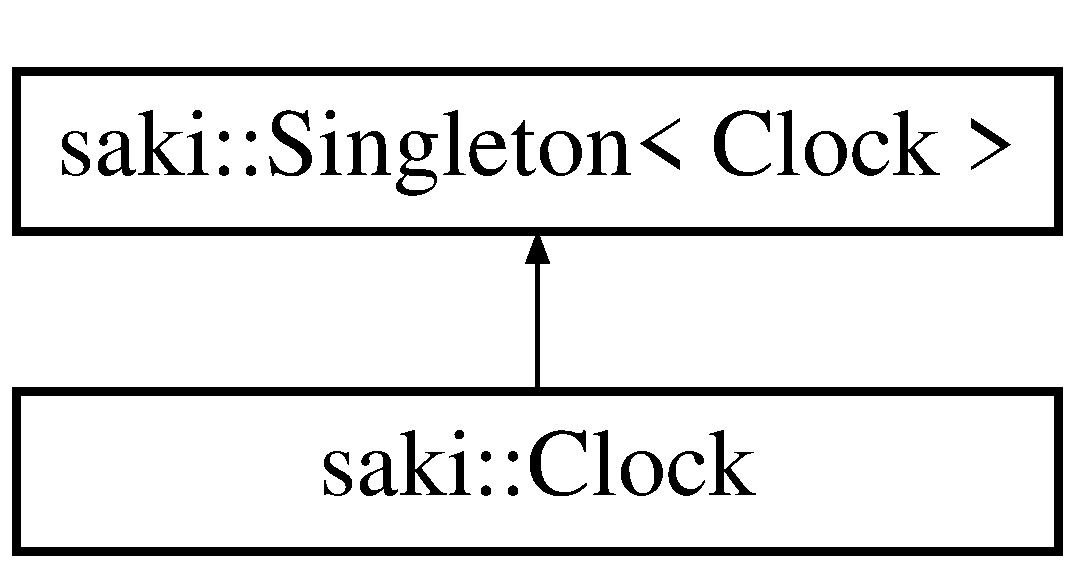
\includegraphics[height=2.000000cm]{classsaki_1_1_clock}
\end{center}
\end{figure}
\subsection*{公開メンバ関数}
\begin{DoxyCompactItemize}
\item 
\mbox{\hyperlink{classsaki_1_1_clock_a235372b9a2044bab90f38c117b49d3ab}{Clock}} ()
\begin{DoxyCompactList}\small\item\em コンストラクタ \end{DoxyCompactList}\item 
void \mbox{\hyperlink{classsaki_1_1_clock_a522e7d5dcae1f457dfc1cd4eb9560cec}{start}} ()
\begin{DoxyCompactList}\small\item\em 開始時間のセット \end{DoxyCompactList}\item 
{\footnotesize template$<$typename T  = double$>$ }\\T \mbox{\hyperlink{classsaki_1_1_clock_afb3a41ac314bb58c010283bea60069f9}{end}} (bool ms=true)
\begin{DoxyCompactList}\small\item\em 開始時間をセットしてからの時間を返す \end{DoxyCompactList}\item 
{\footnotesize template$<$typename T  = double$>$ }\\T \mbox{\hyperlink{classsaki_1_1_clock_a6df6705089065ac8f9f3cdb718d7284f}{end\+\_\+and\+\_\+start}} (bool ms=true)
\begin{DoxyCompactList}\small\item\em 開始時間をセットしてからの時間を返し、そこからまた時間をスタートする \end{DoxyCompactList}\end{DoxyCompactItemize}
\subsection*{その他の継承メンバ}


\subsection{詳解}
時間を測るクラス 

\subsection{構築子と解体子}
\mbox{\Hypertarget{classsaki_1_1_clock_a235372b9a2044bab90f38c117b49d3ab}\label{classsaki_1_1_clock_a235372b9a2044bab90f38c117b49d3ab}} 
\index{saki\+::\+Clock@{saki\+::\+Clock}!Clock@{Clock}}
\index{Clock@{Clock}!saki\+::\+Clock@{saki\+::\+Clock}}
\subsubsection{\texorpdfstring{Clock()}{Clock()}}
{\footnotesize\ttfamily saki\+::\+Clock\+::\+Clock (\begin{DoxyParamCaption}{ }\end{DoxyParamCaption})\hspace{0.3cm}{\ttfamily [inline]}}



コンストラクタ 



\subsection{関数詳解}
\mbox{\Hypertarget{classsaki_1_1_clock_afb3a41ac314bb58c010283bea60069f9}\label{classsaki_1_1_clock_afb3a41ac314bb58c010283bea60069f9}} 
\index{saki\+::\+Clock@{saki\+::\+Clock}!end@{end}}
\index{end@{end}!saki\+::\+Clock@{saki\+::\+Clock}}
\subsubsection{\texorpdfstring{end()}{end()}}
{\footnotesize\ttfamily template$<$typename T  = double$>$ \\
T saki\+::\+Clock\+::end (\begin{DoxyParamCaption}\item[{bool}]{ms = {\ttfamily true} }\end{DoxyParamCaption})\hspace{0.3cm}{\ttfamily [inline]}}



開始時間をセットしてからの時間を返す 


\begin{DoxyParams}{引数}
{\em ms} & trueならミリ秒,falseなら秒で返す return 時間 \\
\hline
\end{DoxyParams}
\mbox{\Hypertarget{classsaki_1_1_clock_a6df6705089065ac8f9f3cdb718d7284f}\label{classsaki_1_1_clock_a6df6705089065ac8f9f3cdb718d7284f}} 
\index{saki\+::\+Clock@{saki\+::\+Clock}!end\+\_\+and\+\_\+start@{end\+\_\+and\+\_\+start}}
\index{end\+\_\+and\+\_\+start@{end\+\_\+and\+\_\+start}!saki\+::\+Clock@{saki\+::\+Clock}}
\subsubsection{\texorpdfstring{end\+\_\+and\+\_\+start()}{end\_and\_start()}}
{\footnotesize\ttfamily template$<$typename T  = double$>$ \\
T saki\+::\+Clock\+::end\+\_\+and\+\_\+start (\begin{DoxyParamCaption}\item[{bool}]{ms = {\ttfamily true} }\end{DoxyParamCaption})\hspace{0.3cm}{\ttfamily [inline]}}



開始時間をセットしてからの時間を返し、そこからまた時間をスタートする 


\begin{DoxyParams}{引数}
{\em ms} & trueならミリ秒,falseなら秒で返す return 時間 \\
\hline
\end{DoxyParams}
\mbox{\Hypertarget{classsaki_1_1_clock_a522e7d5dcae1f457dfc1cd4eb9560cec}\label{classsaki_1_1_clock_a522e7d5dcae1f457dfc1cd4eb9560cec}} 
\index{saki\+::\+Clock@{saki\+::\+Clock}!start@{start}}
\index{start@{start}!saki\+::\+Clock@{saki\+::\+Clock}}
\subsubsection{\texorpdfstring{start()}{start()}}
{\footnotesize\ttfamily void saki\+::\+Clock\+::start (\begin{DoxyParamCaption}{ }\end{DoxyParamCaption})\hspace{0.3cm}{\ttfamily [inline]}}



開始時間のセット 



このクラス詳解は次のファイルから抽出されました\+:\begin{DoxyCompactItemize}
\item 
C\+:/\+Users/tokir/\+Documents/\+Git\+Hub/\+Saki\+Cpp\+Library/saki/clock/\mbox{\hyperlink{clock_8h}{clock.\+h}}\end{DoxyCompactItemize}

\hypertarget{structsaki_1_1division}{}\section{saki\+:\+:division 構造体}
\label{structsaki_1_1division}\index{saki\+::division@{saki\+::division}}


割り算のconstexpr対応した関数オブジェクト  




{\ttfamily \#include $<$division.\+hpp$>$}

\subsection*{公開メンバ関数}
\begin{DoxyCompactItemize}
\item 
{\footnotesize template$<$typename T1 , typename T2 $>$ }\\constexpr auto \mbox{\hyperlink{structsaki_1_1division_a54652339884419a0b696265b17b32705}{operator()}} (const T1 \&t1, const T2 \&t2) const -\/$>$ decltype(t1/t2)
\end{DoxyCompactItemize}


\subsection{詳解}
割り算のconstexpr対応した関数オブジェクト 

\subsection{関数詳解}
\mbox{\Hypertarget{structsaki_1_1division_a54652339884419a0b696265b17b32705}\label{structsaki_1_1division_a54652339884419a0b696265b17b32705}} 
\index{saki\+::division@{saki\+::division}!operator()@{operator()}}
\index{operator()@{operator()}!saki\+::division@{saki\+::division}}
\subsubsection{\texorpdfstring{operator()()}{operator()()}}
{\footnotesize\ttfamily template$<$typename T1 , typename T2 $>$ \\
constexpr auto saki\+::division\+::operator() (\begin{DoxyParamCaption}\item[{const T1 \&}]{t1,  }\item[{const T2 \&}]{t2 }\end{DoxyParamCaption}) const -\/$>$ decltype(t1 / t2)
	\hspace{0.3cm}{\ttfamily [inline]}}



この構造体詳解は次のファイルから抽出されました\+:\begin{DoxyCompactItemize}
\item 
C\+:/\+Users/tokir/\+Documents/\+Git\+Hub/\+Saki\+Cpp\+Library/saki/function\+\_\+object/\mbox{\hyperlink{division_8hpp}{division.\+hpp}}\end{DoxyCompactItemize}

\hypertarget{classsaki_1_1_immobile_ptr}{}\section{saki\+:\+:Immobile\+Ptr$<$ T $>$ クラステンプレート}
\label{classsaki_1_1_immobile_ptr}\index{saki\+::\+Immobile\+Ptr$<$ T $>$@{saki\+::\+Immobile\+Ptr$<$ T $>$}}


コピー・ムーブ禁止のスマートポインタ  




{\ttfamily \#include $<$immobile\+\_\+ptr.\+h$>$}

\subsection*{公開メンバ関数}
\begin{DoxyCompactItemize}
\item 
{\footnotesize template$<$typename ... Args$>$ }\\\mbox{\hyperlink{classsaki_1_1_immobile_ptr_a5b990c72b4222f49b160f4ed5d0c77f9}{Immobile\+Ptr}} (Args... args)
\begin{DoxyCompactList}\small\item\em コンストラクタ時にメモリ確保 \end{DoxyCompactList}\item 
\mbox{\hyperlink{classsaki_1_1_immobile_ptr_ac51507648866a294082a9f38796ca5e4}{$\sim$\+Immobile\+Ptr}} () noexcept
\begin{DoxyCompactList}\small\item\em デストラクタ時にメモリ解放 \end{DoxyCompactList}\item 
void \mbox{\hyperlink{classsaki_1_1_immobile_ptr_a669b89e9c884f703f9dafc1257d694bf}{release}} () noexcept
\begin{DoxyCompactList}\small\item\em 明示的なメモリ解放 \end{DoxyCompactList}\item 
T $\ast$ \mbox{\hyperlink{classsaki_1_1_immobile_ptr_afdaa7016460af66e4e375f064e232720}{get}} ()
\begin{DoxyCompactList}\small\item\em リソースの取得 \end{DoxyCompactList}\item 
T $\ast$$\ast$ \mbox{\hyperlink{classsaki_1_1_immobile_ptr_a8c0dc38fed7ef4e56321909f42f9ed5f}{get\+\_\+address}} ()
\begin{DoxyCompactList}\small\item\em リソースのアドレスを取得 \end{DoxyCompactList}\item 
{\footnotesize template$<$typename ... Args$>$ }\\void \mbox{\hyperlink{classsaki_1_1_immobile_ptr_abc92fb9bf2200ecc6304164ae6c00e09}{reset}} (Args ...args)
\begin{DoxyCompactList}\small\item\em 明示的なメモリ解放と新たにメモリ確保する \end{DoxyCompactList}\item 
\mbox{\hyperlink{classsaki_1_1_immobile_ptr_aa90a657cb5b071d5561ff4f9efe8c979}{operator bool}} () const
\begin{DoxyCompactList}\small\item\em 変換演算子 \end{DoxyCompactList}\item 
T $\ast$ \mbox{\hyperlink{classsaki_1_1_immobile_ptr_a54b22ca7f98168cf42f3b66f3da26006}{operator-\/$>$}} () const
\begin{DoxyCompactList}\small\item\em アロー演算子 \end{DoxyCompactList}\item 
T \mbox{\hyperlink{classsaki_1_1_immobile_ptr_acda7da57ed5dd06c866bd7c96d254cc1}{operator$\ast$}} () const
\begin{DoxyCompactList}\small\item\em 参照演算子 \end{DoxyCompactList}\item 
\mbox{\hyperlink{classsaki_1_1_immobile_ptr_a890a531c0e6371987cfe352196c06d3f}{Immobile\+Ptr}} (const \mbox{\hyperlink{classsaki_1_1_immobile_ptr}{Immobile\+Ptr}} \&)=delete
\item 
\mbox{\hyperlink{classsaki_1_1_immobile_ptr_acfc2a0ddb90c0acaaabfdeb98b10625c}{Immobile\+Ptr}} (\mbox{\hyperlink{classsaki_1_1_immobile_ptr}{Immobile\+Ptr}} \&\&)=delete
\item 
\mbox{\hyperlink{classsaki_1_1_immobile_ptr}{Immobile\+Ptr}} \& \mbox{\hyperlink{classsaki_1_1_immobile_ptr_ad302722791d66a361f6e198696412d4b}{operator=}} (const \mbox{\hyperlink{classsaki_1_1_immobile_ptr}{Immobile\+Ptr}} \&)=delete
\item 
\mbox{\hyperlink{classsaki_1_1_immobile_ptr}{Immobile\+Ptr}} \& \mbox{\hyperlink{classsaki_1_1_immobile_ptr_a115f6cb0829142d395840b921b0df629}{operator=}} (\mbox{\hyperlink{classsaki_1_1_immobile_ptr}{Immobile\+Ptr}} \&\&)=delete
\end{DoxyCompactItemize}


\subsection{詳解}
\subsubsection*{template$<$typename T$>$\newline
class saki\+::\+Immobile\+Ptr$<$ T $>$}

コピー・ムーブ禁止のスマートポインタ 

\subsection{構築子と解体子}
\mbox{\Hypertarget{classsaki_1_1_immobile_ptr_a5b990c72b4222f49b160f4ed5d0c77f9}\label{classsaki_1_1_immobile_ptr_a5b990c72b4222f49b160f4ed5d0c77f9}} 
\index{saki\+::\+Immobile\+Ptr@{saki\+::\+Immobile\+Ptr}!Immobile\+Ptr@{Immobile\+Ptr}}
\index{Immobile\+Ptr@{Immobile\+Ptr}!saki\+::\+Immobile\+Ptr@{saki\+::\+Immobile\+Ptr}}
\subsubsection{\texorpdfstring{Immobile\+Ptr()}{ImmobilePtr()}\hspace{0.1cm}{\footnotesize\ttfamily [1/3]}}
{\footnotesize\ttfamily template$<$typename T $>$ \\
template$<$typename ... Args$>$ \\
\mbox{\hyperlink{classsaki_1_1_immobile_ptr}{saki\+::\+Immobile\+Ptr}}$<$ T $>$\+::\mbox{\hyperlink{classsaki_1_1_immobile_ptr}{Immobile\+Ptr}} (\begin{DoxyParamCaption}\item[{Args...}]{args }\end{DoxyParamCaption})\hspace{0.3cm}{\ttfamily [inline]}, {\ttfamily [explicit]}}



コンストラクタ時にメモリ確保 


\begin{DoxyParams}{引数}
{\em args} & Tのコンストラクタに必要な引数 \\
\hline
\end{DoxyParams}
\mbox{\Hypertarget{classsaki_1_1_immobile_ptr_ac51507648866a294082a9f38796ca5e4}\label{classsaki_1_1_immobile_ptr_ac51507648866a294082a9f38796ca5e4}} 
\index{saki\+::\+Immobile\+Ptr@{saki\+::\+Immobile\+Ptr}!````~Immobile\+Ptr@{$\sim$\+Immobile\+Ptr}}
\index{````~Immobile\+Ptr@{$\sim$\+Immobile\+Ptr}!saki\+::\+Immobile\+Ptr@{saki\+::\+Immobile\+Ptr}}
\subsubsection{\texorpdfstring{$\sim$\+Immobile\+Ptr()}{~ImmobilePtr()}}
{\footnotesize\ttfamily template$<$typename T $>$ \\
\mbox{\hyperlink{classsaki_1_1_immobile_ptr}{saki\+::\+Immobile\+Ptr}}$<$ T $>$\+::$\sim$\mbox{\hyperlink{classsaki_1_1_immobile_ptr}{Immobile\+Ptr}} (\begin{DoxyParamCaption}{ }\end{DoxyParamCaption})\hspace{0.3cm}{\ttfamily [inline]}, {\ttfamily [noexcept]}}



デストラクタ時にメモリ解放 

\mbox{\Hypertarget{classsaki_1_1_immobile_ptr_a890a531c0e6371987cfe352196c06d3f}\label{classsaki_1_1_immobile_ptr_a890a531c0e6371987cfe352196c06d3f}} 
\index{saki\+::\+Immobile\+Ptr@{saki\+::\+Immobile\+Ptr}!Immobile\+Ptr@{Immobile\+Ptr}}
\index{Immobile\+Ptr@{Immobile\+Ptr}!saki\+::\+Immobile\+Ptr@{saki\+::\+Immobile\+Ptr}}
\subsubsection{\texorpdfstring{Immobile\+Ptr()}{ImmobilePtr()}\hspace{0.1cm}{\footnotesize\ttfamily [2/3]}}
{\footnotesize\ttfamily template$<$typename T $>$ \\
\mbox{\hyperlink{classsaki_1_1_immobile_ptr}{saki\+::\+Immobile\+Ptr}}$<$ T $>$\+::\mbox{\hyperlink{classsaki_1_1_immobile_ptr}{Immobile\+Ptr}} (\begin{DoxyParamCaption}\item[{const \mbox{\hyperlink{classsaki_1_1_immobile_ptr}{Immobile\+Ptr}}$<$ T $>$ \&}]{ }\end{DoxyParamCaption})\hspace{0.3cm}{\ttfamily [delete]}}

\mbox{\Hypertarget{classsaki_1_1_immobile_ptr_acfc2a0ddb90c0acaaabfdeb98b10625c}\label{classsaki_1_1_immobile_ptr_acfc2a0ddb90c0acaaabfdeb98b10625c}} 
\index{saki\+::\+Immobile\+Ptr@{saki\+::\+Immobile\+Ptr}!Immobile\+Ptr@{Immobile\+Ptr}}
\index{Immobile\+Ptr@{Immobile\+Ptr}!saki\+::\+Immobile\+Ptr@{saki\+::\+Immobile\+Ptr}}
\subsubsection{\texorpdfstring{Immobile\+Ptr()}{ImmobilePtr()}\hspace{0.1cm}{\footnotesize\ttfamily [3/3]}}
{\footnotesize\ttfamily template$<$typename T $>$ \\
\mbox{\hyperlink{classsaki_1_1_immobile_ptr}{saki\+::\+Immobile\+Ptr}}$<$ T $>$\+::\mbox{\hyperlink{classsaki_1_1_immobile_ptr}{Immobile\+Ptr}} (\begin{DoxyParamCaption}\item[{\mbox{\hyperlink{classsaki_1_1_immobile_ptr}{Immobile\+Ptr}}$<$ T $>$ \&\&}]{ }\end{DoxyParamCaption})\hspace{0.3cm}{\ttfamily [delete]}}



\subsection{関数詳解}
\mbox{\Hypertarget{classsaki_1_1_immobile_ptr_afdaa7016460af66e4e375f064e232720}\label{classsaki_1_1_immobile_ptr_afdaa7016460af66e4e375f064e232720}} 
\index{saki\+::\+Immobile\+Ptr@{saki\+::\+Immobile\+Ptr}!get@{get}}
\index{get@{get}!saki\+::\+Immobile\+Ptr@{saki\+::\+Immobile\+Ptr}}
\subsubsection{\texorpdfstring{get()}{get()}}
{\footnotesize\ttfamily template$<$typename T $>$ \\
T$\ast$ \mbox{\hyperlink{classsaki_1_1_immobile_ptr}{saki\+::\+Immobile\+Ptr}}$<$ T $>$\+::get (\begin{DoxyParamCaption}{ }\end{DoxyParamCaption})\hspace{0.3cm}{\ttfamily [inline]}}



リソースの取得 

\mbox{\Hypertarget{classsaki_1_1_immobile_ptr_a8c0dc38fed7ef4e56321909f42f9ed5f}\label{classsaki_1_1_immobile_ptr_a8c0dc38fed7ef4e56321909f42f9ed5f}} 
\index{saki\+::\+Immobile\+Ptr@{saki\+::\+Immobile\+Ptr}!get\+\_\+address@{get\+\_\+address}}
\index{get\+\_\+address@{get\+\_\+address}!saki\+::\+Immobile\+Ptr@{saki\+::\+Immobile\+Ptr}}
\subsubsection{\texorpdfstring{get\+\_\+address()}{get\_address()}}
{\footnotesize\ttfamily template$<$typename T $>$ \\
T$\ast$$\ast$ \mbox{\hyperlink{classsaki_1_1_immobile_ptr}{saki\+::\+Immobile\+Ptr}}$<$ T $>$\+::get\+\_\+address (\begin{DoxyParamCaption}{ }\end{DoxyParamCaption})\hspace{0.3cm}{\ttfamily [inline]}}



リソースのアドレスを取得 

\mbox{\Hypertarget{classsaki_1_1_immobile_ptr_aa90a657cb5b071d5561ff4f9efe8c979}\label{classsaki_1_1_immobile_ptr_aa90a657cb5b071d5561ff4f9efe8c979}} 
\index{saki\+::\+Immobile\+Ptr@{saki\+::\+Immobile\+Ptr}!operator bool@{operator bool}}
\index{operator bool@{operator bool}!saki\+::\+Immobile\+Ptr@{saki\+::\+Immobile\+Ptr}}
\subsubsection{\texorpdfstring{operator bool()}{operator bool()}}
{\footnotesize\ttfamily template$<$typename T $>$ \\
\mbox{\hyperlink{classsaki_1_1_immobile_ptr}{saki\+::\+Immobile\+Ptr}}$<$ T $>$\+::operator bool (\begin{DoxyParamCaption}{ }\end{DoxyParamCaption}) const\hspace{0.3cm}{\ttfamily [inline]}, {\ttfamily [explicit]}}



変換演算子 

\mbox{\Hypertarget{classsaki_1_1_immobile_ptr_acda7da57ed5dd06c866bd7c96d254cc1}\label{classsaki_1_1_immobile_ptr_acda7da57ed5dd06c866bd7c96d254cc1}} 
\index{saki\+::\+Immobile\+Ptr@{saki\+::\+Immobile\+Ptr}!operator$\ast$@{operator$\ast$}}
\index{operator$\ast$@{operator$\ast$}!saki\+::\+Immobile\+Ptr@{saki\+::\+Immobile\+Ptr}}
\subsubsection{\texorpdfstring{operator$\ast$()}{operator*()}}
{\footnotesize\ttfamily template$<$typename T $>$ \\
T \mbox{\hyperlink{classsaki_1_1_immobile_ptr}{saki\+::\+Immobile\+Ptr}}$<$ T $>$\+::operator$\ast$ (\begin{DoxyParamCaption}{ }\end{DoxyParamCaption}) const\hspace{0.3cm}{\ttfamily [inline]}}



参照演算子 

\mbox{\Hypertarget{classsaki_1_1_immobile_ptr_a54b22ca7f98168cf42f3b66f3da26006}\label{classsaki_1_1_immobile_ptr_a54b22ca7f98168cf42f3b66f3da26006}} 
\index{saki\+::\+Immobile\+Ptr@{saki\+::\+Immobile\+Ptr}!operator-\/$>$@{operator-\/$>$}}
\index{operator-\/$>$@{operator-\/$>$}!saki\+::\+Immobile\+Ptr@{saki\+::\+Immobile\+Ptr}}
\subsubsection{\texorpdfstring{operator-\/$>$()}{operator->()}}
{\footnotesize\ttfamily template$<$typename T $>$ \\
T$\ast$ \mbox{\hyperlink{classsaki_1_1_immobile_ptr}{saki\+::\+Immobile\+Ptr}}$<$ T $>$\+::operator-\/$>$ (\begin{DoxyParamCaption}{ }\end{DoxyParamCaption}) const\hspace{0.3cm}{\ttfamily [inline]}}



アロー演算子 

\mbox{\Hypertarget{classsaki_1_1_immobile_ptr_ad302722791d66a361f6e198696412d4b}\label{classsaki_1_1_immobile_ptr_ad302722791d66a361f6e198696412d4b}} 
\index{saki\+::\+Immobile\+Ptr@{saki\+::\+Immobile\+Ptr}!operator=@{operator=}}
\index{operator=@{operator=}!saki\+::\+Immobile\+Ptr@{saki\+::\+Immobile\+Ptr}}
\subsubsection{\texorpdfstring{operator=()}{operator=()}\hspace{0.1cm}{\footnotesize\ttfamily [1/2]}}
{\footnotesize\ttfamily template$<$typename T $>$ \\
\mbox{\hyperlink{classsaki_1_1_immobile_ptr}{Immobile\+Ptr}}\& \mbox{\hyperlink{classsaki_1_1_immobile_ptr}{saki\+::\+Immobile\+Ptr}}$<$ T $>$\+::operator= (\begin{DoxyParamCaption}\item[{const \mbox{\hyperlink{classsaki_1_1_immobile_ptr}{Immobile\+Ptr}}$<$ T $>$ \&}]{ }\end{DoxyParamCaption})\hspace{0.3cm}{\ttfamily [delete]}}

\mbox{\Hypertarget{classsaki_1_1_immobile_ptr_a115f6cb0829142d395840b921b0df629}\label{classsaki_1_1_immobile_ptr_a115f6cb0829142d395840b921b0df629}} 
\index{saki\+::\+Immobile\+Ptr@{saki\+::\+Immobile\+Ptr}!operator=@{operator=}}
\index{operator=@{operator=}!saki\+::\+Immobile\+Ptr@{saki\+::\+Immobile\+Ptr}}
\subsubsection{\texorpdfstring{operator=()}{operator=()}\hspace{0.1cm}{\footnotesize\ttfamily [2/2]}}
{\footnotesize\ttfamily template$<$typename T $>$ \\
\mbox{\hyperlink{classsaki_1_1_immobile_ptr}{Immobile\+Ptr}}\& \mbox{\hyperlink{classsaki_1_1_immobile_ptr}{saki\+::\+Immobile\+Ptr}}$<$ T $>$\+::operator= (\begin{DoxyParamCaption}\item[{\mbox{\hyperlink{classsaki_1_1_immobile_ptr}{Immobile\+Ptr}}$<$ T $>$ \&\&}]{ }\end{DoxyParamCaption})\hspace{0.3cm}{\ttfamily [delete]}}

\mbox{\Hypertarget{classsaki_1_1_immobile_ptr_a669b89e9c884f703f9dafc1257d694bf}\label{classsaki_1_1_immobile_ptr_a669b89e9c884f703f9dafc1257d694bf}} 
\index{saki\+::\+Immobile\+Ptr@{saki\+::\+Immobile\+Ptr}!release@{release}}
\index{release@{release}!saki\+::\+Immobile\+Ptr@{saki\+::\+Immobile\+Ptr}}
\subsubsection{\texorpdfstring{release()}{release()}}
{\footnotesize\ttfamily template$<$typename T $>$ \\
void \mbox{\hyperlink{classsaki_1_1_immobile_ptr}{saki\+::\+Immobile\+Ptr}}$<$ T $>$\+::release (\begin{DoxyParamCaption}{ }\end{DoxyParamCaption})\hspace{0.3cm}{\ttfamily [inline]}, {\ttfamily [noexcept]}}



明示的なメモリ解放 

\mbox{\Hypertarget{classsaki_1_1_immobile_ptr_abc92fb9bf2200ecc6304164ae6c00e09}\label{classsaki_1_1_immobile_ptr_abc92fb9bf2200ecc6304164ae6c00e09}} 
\index{saki\+::\+Immobile\+Ptr@{saki\+::\+Immobile\+Ptr}!reset@{reset}}
\index{reset@{reset}!saki\+::\+Immobile\+Ptr@{saki\+::\+Immobile\+Ptr}}
\subsubsection{\texorpdfstring{reset()}{reset()}}
{\footnotesize\ttfamily template$<$typename T $>$ \\
template$<$typename ... Args$>$ \\
void \mbox{\hyperlink{classsaki_1_1_immobile_ptr}{saki\+::\+Immobile\+Ptr}}$<$ T $>$\+::reset (\begin{DoxyParamCaption}\item[{Args ...}]{args }\end{DoxyParamCaption})\hspace{0.3cm}{\ttfamily [inline]}}



明示的なメモリ解放と新たにメモリ確保する 


\begin{DoxyParams}{引数}
{\em args} & Tのコンストラクタに必要な引数 \\
\hline
\end{DoxyParams}


このクラス詳解は次のファイルから抽出されました\+:\begin{DoxyCompactItemize}
\item 
C\+:/\+Users/tokir/\+Documents/\+Git\+Hub/\+Saki\+Cpp\+Library/saki/smart\+\_\+ptr/immobile/\mbox{\hyperlink{immobile__ptr_8h}{immobile\+\_\+ptr.\+h}}\end{DoxyCompactItemize}

\hypertarget{classsaki_1_1_matrix}{}\section{saki\+:\+:Matrix$<$ T $>$ クラステンプレート}
\label{classsaki_1_1_matrix}\index{saki\+::\+Matrix$<$ T $>$@{saki\+::\+Matrix$<$ T $>$}}


行列  




{\ttfamily \#include $<$matrix\+\_\+operator.\+h$>$}

\subsection*{公開メンバ関数}
\begin{DoxyCompactItemize}
\item 
constexpr \mbox{\hyperlink{classsaki_1_1_matrix_a820035e9bafc0fa4269c4b94b1ec4f4f}{Matrix}} ()
\begin{DoxyCompactList}\small\item\em 引数なしコンストラクタ \end{DoxyCompactList}\item 
constexpr \mbox{\hyperlink{classsaki_1_1_matrix_ad4f497bd4ba2b7de464afea4436d9a51}{Matrix}} (const T \&m00, const T \&m01, const T \&m02, const T \&m03, const T \&m10, const T \&m11, const T \&m12, const T \&m13, const T \&m20, const T \&m21, const T \&m22, const T \&m23, const T \&m30, const T \&m31, const T \&m32, const T \&m33)
\begin{DoxyCompactList}\small\item\em 引数ありコンストラクタ \end{DoxyCompactList}\item 
constexpr \mbox{\hyperlink{classsaki_1_1_matrix_a945fec9cbcb1b175ac993db6a5c0cbd8}{Matrix}} (const T arr\mbox{[}4\mbox{]}\mbox{[}4\mbox{]})
\begin{DoxyCompactList}\small\item\em 生配列からの初期化 \end{DoxyCompactList}\item 
\mbox{\hyperlink{classsaki_1_1_matrix_a08d28bd14af9be6650325574a20101d7}{Matrix}} (const \mbox{\hyperlink{classsaki_1_1_matrix}{Matrix}}$<$ T $>$ \&)=default
\item 
\mbox{\hyperlink{classsaki_1_1_matrix}{Matrix}}$<$ T $>$ \& \mbox{\hyperlink{classsaki_1_1_matrix_af83ebe0a4f4652fbf30dd64307021603}{operator=}} (const \mbox{\hyperlink{classsaki_1_1_matrix}{Matrix}}$<$ T $>$ \&)=default
\item 
\mbox{\hyperlink{classsaki_1_1_matrix_aced6f31e05917c2c41305dd0be082f8b}{Matrix}} (\mbox{\hyperlink{classsaki_1_1_matrix}{Matrix}}$<$ T $>$ \&\&) noexcept=default
\item 
\mbox{\hyperlink{classsaki_1_1_matrix}{Matrix}} \& \mbox{\hyperlink{classsaki_1_1_matrix_a96b3519d691108a606d4ece3a9bac134}{operator=}} (\mbox{\hyperlink{classsaki_1_1_matrix}{Matrix}}$<$ T $>$ \&\&) noexcept=default
\item 
{\footnotesize template$<$typename U  = T$>$ }\\auto \mbox{\hyperlink{classsaki_1_1_matrix_a06e54f0ce6ff0cd591725a753d9a4c60}{operator+=}} (const \mbox{\hyperlink{classsaki_1_1_matrix}{Matrix}}$<$ U $>$ \&other)
\begin{DoxyCompactList}\small\item\em +=演算子 \end{DoxyCompactList}\item 
{\footnotesize template$<$typename U  = T$>$ }\\auto \mbox{\hyperlink{classsaki_1_1_matrix_a782a94fb837a9973fed259c55e6817f1}{operator-\/=}} (const \mbox{\hyperlink{classsaki_1_1_matrix}{Matrix}}$<$ U $>$ \&other)
\begin{DoxyCompactList}\small\item\em -\/=演算子 \end{DoxyCompactList}\item 
{\footnotesize template$<$typename U  = T$>$ }\\auto \mbox{\hyperlink{classsaki_1_1_matrix_aae1ffee9f67e7c9893a2329c75bd8a51}{operator$\ast$=}} (const U \&scalar)
\begin{DoxyCompactList}\small\item\em $\ast$=演算子(スカラ) \end{DoxyCompactList}\item 
{\footnotesize template$<$typename U  = T$>$ }\\auto \mbox{\hyperlink{classsaki_1_1_matrix_a66c88e0fcf5b1e86180c097ff24ceff4}{operator$\ast$=}} (const \mbox{\hyperlink{classsaki_1_1_matrix}{Matrix}}$<$ U $>$ \&other)
\begin{DoxyCompactList}\small\item\em $\ast$=演算子(行列) \end{DoxyCompactList}\item 
{\footnotesize template$<$typename U  = T$>$ }\\auto \mbox{\hyperlink{classsaki_1_1_matrix_a12f386d5595d02c11a8a7af642183c6c}{operator/=}} (const U \&scalar)
\begin{DoxyCompactList}\small\item\em /=演算子(スカラ) \end{DoxyCompactList}\item 
T $\ast$ \mbox{\hyperlink{classsaki_1_1_matrix_ad1fa9ab13d6ab9def73a4ac5bfa15cf4}{operator\mbox{[}$\,$\mbox{]}}} (const unsigned int index)
\begin{DoxyCompactList}\small\item\em \mbox{[}\mbox{]}演算子 \end{DoxyCompactList}\item 
constexpr T \mbox{\hyperlink{classsaki_1_1_matrix_ac9e6609628221255fd9577eceb9ab2af}{at\+\_\+constexpr}} (const unsigned int row, const unsigned int col) const
\begin{DoxyCompactList}\small\item\em \mbox{[}\mbox{]}演算子では表現できないため、普通の関数にした \end{DoxyCompactList}\item 
void \mbox{\hyperlink{classsaki_1_1_matrix_af0c4f3614c29e27eae5fecde22140be8}{identity}} ()
\begin{DoxyCompactList}\small\item\em 単位行列に変換 \end{DoxyCompactList}\end{DoxyCompactItemize}


\subsection{詳解}
\subsubsection*{template$<$typename T$>$\newline
class saki\+::\+Matrix$<$ T $>$}

行列 

\subsection{構築子と解体子}
\mbox{\Hypertarget{classsaki_1_1_matrix_a820035e9bafc0fa4269c4b94b1ec4f4f}\label{classsaki_1_1_matrix_a820035e9bafc0fa4269c4b94b1ec4f4f}} 
\index{saki\+::\+Matrix@{saki\+::\+Matrix}!Matrix@{Matrix}}
\index{Matrix@{Matrix}!saki\+::\+Matrix@{saki\+::\+Matrix}}
\subsubsection{\texorpdfstring{Matrix()}{Matrix()}\hspace{0.1cm}{\footnotesize\ttfamily [1/5]}}
{\footnotesize\ttfamily template$<$typename T$>$ \\
constexpr \mbox{\hyperlink{classsaki_1_1_matrix}{saki\+::\+Matrix}}$<$ T $>$\+::\mbox{\hyperlink{classsaki_1_1_matrix}{Matrix}} (\begin{DoxyParamCaption}{ }\end{DoxyParamCaption})\hspace{0.3cm}{\ttfamily [inline]}}



引数なしコンストラクタ 

全て0で初期化 \mbox{\Hypertarget{classsaki_1_1_matrix_ad4f497bd4ba2b7de464afea4436d9a51}\label{classsaki_1_1_matrix_ad4f497bd4ba2b7de464afea4436d9a51}} 
\index{saki\+::\+Matrix@{saki\+::\+Matrix}!Matrix@{Matrix}}
\index{Matrix@{Matrix}!saki\+::\+Matrix@{saki\+::\+Matrix}}
\subsubsection{\texorpdfstring{Matrix()}{Matrix()}\hspace{0.1cm}{\footnotesize\ttfamily [2/5]}}
{\footnotesize\ttfamily template$<$typename T$>$ \\
constexpr \mbox{\hyperlink{classsaki_1_1_matrix}{saki\+::\+Matrix}}$<$ T $>$\+::\mbox{\hyperlink{classsaki_1_1_matrix}{Matrix}} (\begin{DoxyParamCaption}\item[{const T \&}]{m00,  }\item[{const T \&}]{m01,  }\item[{const T \&}]{m02,  }\item[{const T \&}]{m03,  }\item[{const T \&}]{m10,  }\item[{const T \&}]{m11,  }\item[{const T \&}]{m12,  }\item[{const T \&}]{m13,  }\item[{const T \&}]{m20,  }\item[{const T \&}]{m21,  }\item[{const T \&}]{m22,  }\item[{const T \&}]{m23,  }\item[{const T \&}]{m30,  }\item[{const T \&}]{m31,  }\item[{const T \&}]{m32,  }\item[{const T \&}]{m33 }\end{DoxyParamCaption})\hspace{0.3cm}{\ttfamily [inline]}}



引数ありコンストラクタ 

\mbox{\Hypertarget{classsaki_1_1_matrix_a945fec9cbcb1b175ac993db6a5c0cbd8}\label{classsaki_1_1_matrix_a945fec9cbcb1b175ac993db6a5c0cbd8}} 
\index{saki\+::\+Matrix@{saki\+::\+Matrix}!Matrix@{Matrix}}
\index{Matrix@{Matrix}!saki\+::\+Matrix@{saki\+::\+Matrix}}
\subsubsection{\texorpdfstring{Matrix()}{Matrix()}\hspace{0.1cm}{\footnotesize\ttfamily [3/5]}}
{\footnotesize\ttfamily template$<$typename T$>$ \\
constexpr \mbox{\hyperlink{classsaki_1_1_matrix}{saki\+::\+Matrix}}$<$ T $>$\+::\mbox{\hyperlink{classsaki_1_1_matrix}{Matrix}} (\begin{DoxyParamCaption}\item[{const T}]{arr\mbox{[}4\mbox{]}\mbox{[}4\mbox{]} }\end{DoxyParamCaption})\hspace{0.3cm}{\ttfamily [inline]}}



生配列からの初期化 


\begin{DoxyParams}{引数}
{\em arr} & 4$\ast$4の配列 \\
\hline
\end{DoxyParams}
\mbox{\Hypertarget{classsaki_1_1_matrix_a08d28bd14af9be6650325574a20101d7}\label{classsaki_1_1_matrix_a08d28bd14af9be6650325574a20101d7}} 
\index{saki\+::\+Matrix@{saki\+::\+Matrix}!Matrix@{Matrix}}
\index{Matrix@{Matrix}!saki\+::\+Matrix@{saki\+::\+Matrix}}
\subsubsection{\texorpdfstring{Matrix()}{Matrix()}\hspace{0.1cm}{\footnotesize\ttfamily [4/5]}}
{\footnotesize\ttfamily template$<$typename T$>$ \\
\mbox{\hyperlink{classsaki_1_1_matrix}{saki\+::\+Matrix}}$<$ T $>$\+::\mbox{\hyperlink{classsaki_1_1_matrix}{Matrix}} (\begin{DoxyParamCaption}\item[{const \mbox{\hyperlink{classsaki_1_1_matrix}{Matrix}}$<$ T $>$ \&}]{ }\end{DoxyParamCaption})\hspace{0.3cm}{\ttfamily [default]}}

\mbox{\Hypertarget{classsaki_1_1_matrix_aced6f31e05917c2c41305dd0be082f8b}\label{classsaki_1_1_matrix_aced6f31e05917c2c41305dd0be082f8b}} 
\index{saki\+::\+Matrix@{saki\+::\+Matrix}!Matrix@{Matrix}}
\index{Matrix@{Matrix}!saki\+::\+Matrix@{saki\+::\+Matrix}}
\subsubsection{\texorpdfstring{Matrix()}{Matrix()}\hspace{0.1cm}{\footnotesize\ttfamily [5/5]}}
{\footnotesize\ttfamily template$<$typename T$>$ \\
\mbox{\hyperlink{classsaki_1_1_matrix}{saki\+::\+Matrix}}$<$ T $>$\+::\mbox{\hyperlink{classsaki_1_1_matrix}{Matrix}} (\begin{DoxyParamCaption}\item[{\mbox{\hyperlink{classsaki_1_1_matrix}{Matrix}}$<$ T $>$ \&\&}]{ }\end{DoxyParamCaption})\hspace{0.3cm}{\ttfamily [default]}, {\ttfamily [noexcept]}}



\subsection{関数詳解}
\mbox{\Hypertarget{classsaki_1_1_matrix_ac9e6609628221255fd9577eceb9ab2af}\label{classsaki_1_1_matrix_ac9e6609628221255fd9577eceb9ab2af}} 
\index{saki\+::\+Matrix@{saki\+::\+Matrix}!at\+\_\+constexpr@{at\+\_\+constexpr}}
\index{at\+\_\+constexpr@{at\+\_\+constexpr}!saki\+::\+Matrix@{saki\+::\+Matrix}}
\subsubsection{\texorpdfstring{at\+\_\+constexpr()}{at\_constexpr()}}
{\footnotesize\ttfamily template$<$typename T$>$ \\
constexpr T \mbox{\hyperlink{classsaki_1_1_matrix}{saki\+::\+Matrix}}$<$ T $>$\+::at\+\_\+constexpr (\begin{DoxyParamCaption}\item[{const unsigned int}]{row,  }\item[{const unsigned int}]{col }\end{DoxyParamCaption}) const\hspace{0.3cm}{\ttfamily [inline]}}



\mbox{[}\mbox{]}演算子では表現できないため、普通の関数にした 


\begin{DoxyParams}{引数}
{\em row,col} & 行、列\\
\hline
\end{DoxyParams}
自作arrayクラスを作成すればできるが、とりあえず今はこのままで \mbox{\Hypertarget{classsaki_1_1_matrix_af0c4f3614c29e27eae5fecde22140be8}\label{classsaki_1_1_matrix_af0c4f3614c29e27eae5fecde22140be8}} 
\index{saki\+::\+Matrix@{saki\+::\+Matrix}!identity@{identity}}
\index{identity@{identity}!saki\+::\+Matrix@{saki\+::\+Matrix}}
\subsubsection{\texorpdfstring{identity()}{identity()}}
{\footnotesize\ttfamily template$<$typename T$>$ \\
void \mbox{\hyperlink{classsaki_1_1_matrix}{saki\+::\+Matrix}}$<$ T $>$\+::identity (\begin{DoxyParamCaption}{ }\end{DoxyParamCaption})\hspace{0.3cm}{\ttfamily [inline]}}



単位行列に変換 

\mbox{\Hypertarget{classsaki_1_1_matrix_aae1ffee9f67e7c9893a2329c75bd8a51}\label{classsaki_1_1_matrix_aae1ffee9f67e7c9893a2329c75bd8a51}} 
\index{saki\+::\+Matrix@{saki\+::\+Matrix}!operator$\ast$=@{operator$\ast$=}}
\index{operator$\ast$=@{operator$\ast$=}!saki\+::\+Matrix@{saki\+::\+Matrix}}
\subsubsection{\texorpdfstring{operator$\ast$=()}{operator*=()}\hspace{0.1cm}{\footnotesize\ttfamily [1/2]}}
{\footnotesize\ttfamily template$<$typename T$>$ \\
template$<$typename U  = T$>$ \\
auto \mbox{\hyperlink{classsaki_1_1_matrix}{saki\+::\+Matrix}}$<$ T $>$\+::operator$\ast$= (\begin{DoxyParamCaption}\item[{const U \&}]{scalar }\end{DoxyParamCaption})\hspace{0.3cm}{\ttfamily [inline]}}



$\ast$=演算子(スカラ) 

\mbox{\Hypertarget{classsaki_1_1_matrix_a66c88e0fcf5b1e86180c097ff24ceff4}\label{classsaki_1_1_matrix_a66c88e0fcf5b1e86180c097ff24ceff4}} 
\index{saki\+::\+Matrix@{saki\+::\+Matrix}!operator$\ast$=@{operator$\ast$=}}
\index{operator$\ast$=@{operator$\ast$=}!saki\+::\+Matrix@{saki\+::\+Matrix}}
\subsubsection{\texorpdfstring{operator$\ast$=()}{operator*=()}\hspace{0.1cm}{\footnotesize\ttfamily [2/2]}}
{\footnotesize\ttfamily template$<$typename T$>$ \\
template$<$typename U  = T$>$ \\
auto \mbox{\hyperlink{classsaki_1_1_matrix}{saki\+::\+Matrix}}$<$ T $>$\+::operator$\ast$= (\begin{DoxyParamCaption}\item[{const \mbox{\hyperlink{classsaki_1_1_matrix}{Matrix}}$<$ U $>$ \&}]{other }\end{DoxyParamCaption})\hspace{0.3cm}{\ttfamily [inline]}}



$\ast$=演算子(行列) 

\mbox{\Hypertarget{classsaki_1_1_matrix_a06e54f0ce6ff0cd591725a753d9a4c60}\label{classsaki_1_1_matrix_a06e54f0ce6ff0cd591725a753d9a4c60}} 
\index{saki\+::\+Matrix@{saki\+::\+Matrix}!operator+=@{operator+=}}
\index{operator+=@{operator+=}!saki\+::\+Matrix@{saki\+::\+Matrix}}
\subsubsection{\texorpdfstring{operator+=()}{operator+=()}}
{\footnotesize\ttfamily template$<$typename T$>$ \\
template$<$typename U  = T$>$ \\
auto \mbox{\hyperlink{classsaki_1_1_matrix}{saki\+::\+Matrix}}$<$ T $>$\+::operator+= (\begin{DoxyParamCaption}\item[{const \mbox{\hyperlink{classsaki_1_1_matrix}{Matrix}}$<$ U $>$ \&}]{other }\end{DoxyParamCaption})\hspace{0.3cm}{\ttfamily [inline]}}



+=演算子 

\mbox{\Hypertarget{classsaki_1_1_matrix_a782a94fb837a9973fed259c55e6817f1}\label{classsaki_1_1_matrix_a782a94fb837a9973fed259c55e6817f1}} 
\index{saki\+::\+Matrix@{saki\+::\+Matrix}!operator-\/=@{operator-\/=}}
\index{operator-\/=@{operator-\/=}!saki\+::\+Matrix@{saki\+::\+Matrix}}
\subsubsection{\texorpdfstring{operator-\/=()}{operator-=()}}
{\footnotesize\ttfamily template$<$typename T$>$ \\
template$<$typename U  = T$>$ \\
auto \mbox{\hyperlink{classsaki_1_1_matrix}{saki\+::\+Matrix}}$<$ T $>$\+::operator-\/= (\begin{DoxyParamCaption}\item[{const \mbox{\hyperlink{classsaki_1_1_matrix}{Matrix}}$<$ U $>$ \&}]{other }\end{DoxyParamCaption})\hspace{0.3cm}{\ttfamily [inline]}}



-\/=演算子 

\mbox{\Hypertarget{classsaki_1_1_matrix_a12f386d5595d02c11a8a7af642183c6c}\label{classsaki_1_1_matrix_a12f386d5595d02c11a8a7af642183c6c}} 
\index{saki\+::\+Matrix@{saki\+::\+Matrix}!operator/=@{operator/=}}
\index{operator/=@{operator/=}!saki\+::\+Matrix@{saki\+::\+Matrix}}
\subsubsection{\texorpdfstring{operator/=()}{operator/=()}}
{\footnotesize\ttfamily template$<$typename T$>$ \\
template$<$typename U  = T$>$ \\
auto \mbox{\hyperlink{classsaki_1_1_matrix}{saki\+::\+Matrix}}$<$ T $>$\+::operator/= (\begin{DoxyParamCaption}\item[{const U \&}]{scalar }\end{DoxyParamCaption})\hspace{0.3cm}{\ttfamily [inline]}}



/=演算子(スカラ) 

\mbox{\Hypertarget{classsaki_1_1_matrix_af83ebe0a4f4652fbf30dd64307021603}\label{classsaki_1_1_matrix_af83ebe0a4f4652fbf30dd64307021603}} 
\index{saki\+::\+Matrix@{saki\+::\+Matrix}!operator=@{operator=}}
\index{operator=@{operator=}!saki\+::\+Matrix@{saki\+::\+Matrix}}
\subsubsection{\texorpdfstring{operator=()}{operator=()}\hspace{0.1cm}{\footnotesize\ttfamily [1/2]}}
{\footnotesize\ttfamily template$<$typename T$>$ \\
\mbox{\hyperlink{classsaki_1_1_matrix}{Matrix}}$<$T$>$\& \mbox{\hyperlink{classsaki_1_1_matrix}{saki\+::\+Matrix}}$<$ T $>$\+::operator= (\begin{DoxyParamCaption}\item[{const \mbox{\hyperlink{classsaki_1_1_matrix}{Matrix}}$<$ T $>$ \&}]{ }\end{DoxyParamCaption})\hspace{0.3cm}{\ttfamily [default]}}

\mbox{\Hypertarget{classsaki_1_1_matrix_a96b3519d691108a606d4ece3a9bac134}\label{classsaki_1_1_matrix_a96b3519d691108a606d4ece3a9bac134}} 
\index{saki\+::\+Matrix@{saki\+::\+Matrix}!operator=@{operator=}}
\index{operator=@{operator=}!saki\+::\+Matrix@{saki\+::\+Matrix}}
\subsubsection{\texorpdfstring{operator=()}{operator=()}\hspace{0.1cm}{\footnotesize\ttfamily [2/2]}}
{\footnotesize\ttfamily template$<$typename T$>$ \\
\mbox{\hyperlink{classsaki_1_1_matrix}{Matrix}}\& \mbox{\hyperlink{classsaki_1_1_matrix}{saki\+::\+Matrix}}$<$ T $>$\+::operator= (\begin{DoxyParamCaption}\item[{\mbox{\hyperlink{classsaki_1_1_matrix}{Matrix}}$<$ T $>$ \&\&}]{ }\end{DoxyParamCaption})\hspace{0.3cm}{\ttfamily [default]}, {\ttfamily [noexcept]}}

\mbox{\Hypertarget{classsaki_1_1_matrix_ad1fa9ab13d6ab9def73a4ac5bfa15cf4}\label{classsaki_1_1_matrix_ad1fa9ab13d6ab9def73a4ac5bfa15cf4}} 
\index{saki\+::\+Matrix@{saki\+::\+Matrix}!operator\mbox{[}\mbox{]}@{operator[]}}
\index{operator\mbox{[}\mbox{]}@{operator[]}!saki\+::\+Matrix@{saki\+::\+Matrix}}
\subsubsection{\texorpdfstring{operator[]()}{operator[]()}}
{\footnotesize\ttfamily template$<$typename T$>$ \\
T$\ast$ \mbox{\hyperlink{classsaki_1_1_matrix}{saki\+::\+Matrix}}$<$ T $>$\+::operator\mbox{[}$\,$\mbox{]} (\begin{DoxyParamCaption}\item[{const unsigned int}]{index }\end{DoxyParamCaption})\hspace{0.3cm}{\ttfamily [inline]}}



\mbox{[}\mbox{]}演算子 



このクラス詳解は次のファイルから抽出されました\+:\begin{DoxyCompactItemize}
\item 
C\+:/\+Users/tokir/\+Documents/\+Git\+Hub/\+Saki\+Cpp\+Library/saki/matrix/details/\mbox{\hyperlink{matrix__operator_8h}{matrix\+\_\+operator.\+h}}\item 
C\+:/\+Users/tokir/\+Documents/\+Git\+Hub/\+Saki\+Cpp\+Library/saki/matrix/\mbox{\hyperlink{matrix_8h}{matrix.\+h}}\end{DoxyCompactItemize}

\hypertarget{structsaki_1_1multiplication}{}\section{saki\+:\+:multiplication 構造体}
\label{structsaki_1_1multiplication}\index{saki\+::multiplication@{saki\+::multiplication}}


掛け算のconstexpr対応した関数オブジェクト  




{\ttfamily \#include $<$multiplication.\+h$>$}

\subsection*{公開メンバ関数}
\begin{DoxyCompactItemize}
\item 
{\footnotesize template$<$typename T1 , typename T2 $>$ }\\constexpr auto \mbox{\hyperlink{structsaki_1_1multiplication_ad7c9cfc08911b6db3ea95d4cfd5ffa7f}{operator()}} (const T1 \&t1, const T2 \&t2) const
\end{DoxyCompactItemize}


\subsection{詳解}
掛け算のconstexpr対応した関数オブジェクト 

\subsection{関数詳解}
\mbox{\Hypertarget{structsaki_1_1multiplication_ad7c9cfc08911b6db3ea95d4cfd5ffa7f}\label{structsaki_1_1multiplication_ad7c9cfc08911b6db3ea95d4cfd5ffa7f}} 
\index{saki\+::multiplication@{saki\+::multiplication}!operator()@{operator()}}
\index{operator()@{operator()}!saki\+::multiplication@{saki\+::multiplication}}
\subsubsection{\texorpdfstring{operator()()}{operator()()}}
{\footnotesize\ttfamily template$<$typename T1 , typename T2 $>$ \\
constexpr auto saki\+::multiplication\+::operator() (\begin{DoxyParamCaption}\item[{const T1 \&}]{t1,  }\item[{const T2 \&}]{t2 }\end{DoxyParamCaption}) const\hspace{0.3cm}{\ttfamily [inline]}}



この構造体詳解は次のファイルから抽出されました\+:\begin{DoxyCompactItemize}
\item 
C\+:/\+Users/tokir/\+Documents/\+Git\+Hub/\+Saki\+Cpp\+Library/saki/function\+\_\+object/\mbox{\hyperlink{multiplication_8h}{multiplication.\+h}}\end{DoxyCompactItemize}

\hypertarget{structsaki_1_1_return_param}{}\section{saki\+:\+:Return\+Param 構造体}
\label{structsaki_1_1_return_param}\index{saki\+::\+Return\+Param@{saki\+::\+Return\+Param}}


そのまま引数を返す関数オブジェクト  




{\ttfamily \#include $<$return\+\_\+param.\+h$>$}

\subsection*{公開メンバ関数}
\begin{DoxyCompactItemize}
\item 
{\footnotesize template$<$typename T $>$ }\\constexpr T \mbox{\hyperlink{structsaki_1_1_return_param_aee3b0cc7bc68a43e72cae1a988d5c46b}{operator()}} (const T \&t)
\end{DoxyCompactItemize}


\subsection{詳解}
そのまま引数を返す関数オブジェクト 

\subsection{関数詳解}
\mbox{\Hypertarget{structsaki_1_1_return_param_aee3b0cc7bc68a43e72cae1a988d5c46b}\label{structsaki_1_1_return_param_aee3b0cc7bc68a43e72cae1a988d5c46b}} 
\index{saki\+::\+Return\+Param@{saki\+::\+Return\+Param}!operator()@{operator()}}
\index{operator()@{operator()}!saki\+::\+Return\+Param@{saki\+::\+Return\+Param}}
\subsubsection{\texorpdfstring{operator()()}{operator()()}}
{\footnotesize\ttfamily template$<$typename T $>$ \\
constexpr T saki\+::\+Return\+Param\+::operator() (\begin{DoxyParamCaption}\item[{const T \&}]{t }\end{DoxyParamCaption})\hspace{0.3cm}{\ttfamily [inline]}}



この構造体詳解は次のファイルから抽出されました\+:\begin{DoxyCompactItemize}
\item 
C\+:/\+Users/tokir/\+Documents/\+Git\+Hub/\+Saki\+Cpp\+Library/saki/binary\+\_\+operator/\mbox{\hyperlink{return__param_8h}{return\+\_\+param.\+h}}\end{DoxyCompactItemize}

\hypertarget{classsaki_1_1_singleton}{}\section{saki\+:\+:Singleton$<$ T $>$ クラステンプレート}
\label{classsaki_1_1_singleton}\index{saki\+::\+Singleton$<$ T $>$@{saki\+::\+Singleton$<$ T $>$}}


継承するとシングルトンクラスになる  




{\ttfamily \#include $<$singleton.\+h$>$}

\subsection*{公開メンバ関数}
\begin{DoxyCompactItemize}
\item 
virtual \mbox{\hyperlink{classsaki_1_1_singleton_a3ff92ba5c83fba36d539cfa16d35599a}{$\sim$\+Singleton}} ()
\end{DoxyCompactItemize}
\subsection*{静的公開メンバ関数}
\begin{DoxyCompactItemize}
\item 
static std\+::unique\+\_\+ptr$<$ T $>$ \& \mbox{\hyperlink{classsaki_1_1_singleton_a198911b1e5a72914511ffd6f50e4da2f}{getinstance}} ()
\begin{DoxyCompactList}\small\item\em インスタンスを取得 \end{DoxyCompactList}\end{DoxyCompactItemize}
\subsection*{限定公開メンバ関数}
\begin{DoxyCompactItemize}
\item 
\mbox{\hyperlink{classsaki_1_1_singleton_a1cd9f69783e3c0c83db851edc061bb7f}{Singleton}} ()
\end{DoxyCompactItemize}


\subsection{詳解}
\subsubsection*{template$<$typename T$>$\newline
class saki\+::\+Singleton$<$ T $>$}

継承するとシングルトンクラスになる 

\subsection{構築子と解体子}
\mbox{\Hypertarget{classsaki_1_1_singleton_a3ff92ba5c83fba36d539cfa16d35599a}\label{classsaki_1_1_singleton_a3ff92ba5c83fba36d539cfa16d35599a}} 
\index{saki\+::\+Singleton@{saki\+::\+Singleton}!````~Singleton@{$\sim$\+Singleton}}
\index{````~Singleton@{$\sim$\+Singleton}!saki\+::\+Singleton@{saki\+::\+Singleton}}
\subsubsection{\texorpdfstring{$\sim$\+Singleton()}{~Singleton()}}
{\footnotesize\ttfamily template$<$typename T$>$ \\
virtual \mbox{\hyperlink{classsaki_1_1_singleton}{saki\+::\+Singleton}}$<$ T $>$\+::$\sim$\mbox{\hyperlink{classsaki_1_1_singleton}{Singleton}} (\begin{DoxyParamCaption}{ }\end{DoxyParamCaption})\hspace{0.3cm}{\ttfamily [inline]}, {\ttfamily [virtual]}}

\mbox{\Hypertarget{classsaki_1_1_singleton_a1cd9f69783e3c0c83db851edc061bb7f}\label{classsaki_1_1_singleton_a1cd9f69783e3c0c83db851edc061bb7f}} 
\index{saki\+::\+Singleton@{saki\+::\+Singleton}!Singleton@{Singleton}}
\index{Singleton@{Singleton}!saki\+::\+Singleton@{saki\+::\+Singleton}}
\subsubsection{\texorpdfstring{Singleton()}{Singleton()}}
{\footnotesize\ttfamily template$<$typename T$>$ \\
\mbox{\hyperlink{classsaki_1_1_singleton}{saki\+::\+Singleton}}$<$ T $>$\+::\mbox{\hyperlink{classsaki_1_1_singleton}{Singleton}} (\begin{DoxyParamCaption}{ }\end{DoxyParamCaption})\hspace{0.3cm}{\ttfamily [inline]}, {\ttfamily [protected]}}



\subsection{関数詳解}
\mbox{\Hypertarget{classsaki_1_1_singleton_a198911b1e5a72914511ffd6f50e4da2f}\label{classsaki_1_1_singleton_a198911b1e5a72914511ffd6f50e4da2f}} 
\index{saki\+::\+Singleton@{saki\+::\+Singleton}!getinstance@{getinstance}}
\index{getinstance@{getinstance}!saki\+::\+Singleton@{saki\+::\+Singleton}}
\subsubsection{\texorpdfstring{getinstance()}{getinstance()}}
{\footnotesize\ttfamily template$<$typename T$>$ \\
static std\+::unique\+\_\+ptr$<$T$>$\& \mbox{\hyperlink{classsaki_1_1_singleton}{saki\+::\+Singleton}}$<$ T $>$\+::getinstance (\begin{DoxyParamCaption}{ }\end{DoxyParamCaption})\hspace{0.3cm}{\ttfamily [inline]}, {\ttfamily [static]}}



インスタンスを取得 

\begin{DoxyReturn}{戻り値}
std\+::unique\+\_\+ptr$<$\+T$>$ インスタンスを返す 
\end{DoxyReturn}


このクラス詳解は次のファイルから抽出されました\+:\begin{DoxyCompactItemize}
\item 
C\+:/\+Users/tokir/\+Documents/\+Git\+Hub/\+Saki\+Cpp\+Library/saki/singleton/\mbox{\hyperlink{singleton_8h}{singleton.\+h}}\end{DoxyCompactItemize}

\hypertarget{structsaki_1_1subtraction}{}\section{saki\+:\+:subtraction 構造体}
\label{structsaki_1_1subtraction}\index{saki\+::subtraction@{saki\+::subtraction}}


引き算のconstexpr対応した関数オブジェクト  




{\ttfamily \#include $<$subtraction.\+hpp$>$}

\subsection*{公開メンバ関数}
\begin{DoxyCompactItemize}
\item 
{\footnotesize template$<$typename T1 , typename T2 $>$ }\\constexpr auto \mbox{\hyperlink{structsaki_1_1subtraction_a5de4626c125df92e70848fcac27eef74}{operator()}} (const T1 \&t1, const T2 \&t2) const -\/$>$ decltype(t1 -\/ t2)
\end{DoxyCompactItemize}


\subsection{詳解}
引き算のconstexpr対応した関数オブジェクト 

\subsection{関数詳解}
\mbox{\Hypertarget{structsaki_1_1subtraction_a5de4626c125df92e70848fcac27eef74}\label{structsaki_1_1subtraction_a5de4626c125df92e70848fcac27eef74}} 
\index{saki\+::subtraction@{saki\+::subtraction}!operator()@{operator()}}
\index{operator()@{operator()}!saki\+::subtraction@{saki\+::subtraction}}
\subsubsection{\texorpdfstring{operator()()}{operator()()}}
{\footnotesize\ttfamily template$<$typename T1 , typename T2 $>$ \\
constexpr auto saki\+::subtraction\+::operator() (\begin{DoxyParamCaption}\item[{const T1 \&}]{t1,  }\item[{const T2 \&}]{t2 }\end{DoxyParamCaption}) const -\/$>$ decltype(t1 -\/ t2)
	\hspace{0.3cm}{\ttfamily [inline]}}



この構造体詳解は次のファイルから抽出されました\+:\begin{DoxyCompactItemize}
\item 
C\+:/\+Users/tokir/\+Documents/\+Git\+Hub/\+Saki\+Cpp\+Library/saki/function\+\_\+object/\mbox{\hyperlink{subtraction_8hpp}{subtraction.\+hpp}}\end{DoxyCompactItemize}

\hypertarget{classsaki_1_1_vector2}{}\section{saki\+:\+:Vector2$<$ T $>$ クラステンプレート}
\label{classsaki_1_1_vector2}\index{saki\+::\+Vector2$<$ T $>$@{saki\+::\+Vector2$<$ T $>$}}


2次元でのベクトル  




{\ttfamily \#include $<$vector\+\_\+2d.\+h$>$}

\subsection*{公開メンバ関数}
\begin{DoxyCompactItemize}
\item 
constexpr \mbox{\hyperlink{classsaki_1_1_vector2_af57b72f4255812a361bef1922a226f86}{Vector2}} ()
\begin{DoxyCompactList}\small\item\em 引数なしコンストラクタ \end{DoxyCompactList}\item 
constexpr \mbox{\hyperlink{classsaki_1_1_vector2_ad0f3d0a05370f1ef4947520245f6e9a8}{Vector2}} (const T \&\+\_\+x, const T \&\+\_\+y)
\begin{DoxyCompactList}\small\item\em 引数ありコンストラクタ \end{DoxyCompactList}\item 
constexpr \mbox{\hyperlink{classsaki_1_1_vector2_ad2c0fd66544f68066179490647244b14}{Vector2}} (const T $\ast$const pointer)
\begin{DoxyCompactList}\small\item\em 生配列からの初期化 \end{DoxyCompactList}\item 
\mbox{\hyperlink{classsaki_1_1_vector2_af3d61bb90047a8621cba0a17b265bfaa}{Vector2}} (const \mbox{\hyperlink{classsaki_1_1_vector2}{Vector2}}$<$ T $>$ \&)=default
\item 
\mbox{\hyperlink{classsaki_1_1_vector2}{Vector2}}$<$ T $>$ \& \mbox{\hyperlink{classsaki_1_1_vector2_ae6ee2a6387bfe58bdd5bf74d388370a9}{operator=}} (const \mbox{\hyperlink{classsaki_1_1_vector2}{Vector2}}$<$ T $>$ \&)=default
\item 
\mbox{\hyperlink{classsaki_1_1_vector2_ade059efe536b29346642aacbd973d062}{Vector2}} (\mbox{\hyperlink{classsaki_1_1_vector2}{Vector2}}$<$ T $>$ \&\&) noexcept=default
\item 
\mbox{\hyperlink{classsaki_1_1_vector2}{Vector2}} \& \mbox{\hyperlink{classsaki_1_1_vector2_a5cc432dc740f218177bd028a5899939f}{operator=}} (\mbox{\hyperlink{classsaki_1_1_vector2}{Vector2}}$<$ T $>$ \&\&) noexcept=default
\item 
{\footnotesize template$<$typename U  = T$>$ }\\auto \mbox{\hyperlink{classsaki_1_1_vector2_aa76ccb2d2228441d510dca7781f785d3}{operator+=}} (const \mbox{\hyperlink{classsaki_1_1_vector2}{Vector2}}$<$ U $>$ \&other)
\begin{DoxyCompactList}\small\item\em +=演算子 \end{DoxyCompactList}\item 
{\footnotesize template$<$typename U  = T$>$ }\\auto \mbox{\hyperlink{classsaki_1_1_vector2_aaf222bfb3a2e02a1570ce2e90c41fdd0}{operator-\/=}} (const \mbox{\hyperlink{classsaki_1_1_vector2}{Vector2}}$<$ U $>$ \&other)
\begin{DoxyCompactList}\small\item\em -\/=演算子 \end{DoxyCompactList}\item 
{\footnotesize template$<$typename U  = T$>$ }\\auto \mbox{\hyperlink{classsaki_1_1_vector2_aab202f42563239dfb59d27295d6c7462}{operator$\ast$=}} (const U \&scalar)
\begin{DoxyCompactList}\small\item\em $\ast$=演算子(スカラ) \end{DoxyCompactList}\item 
{\footnotesize template$<$typename U  = T$>$ }\\auto \mbox{\hyperlink{classsaki_1_1_vector2_a31e1e9e5918b362e2559b453da787fbb}{operator$\ast$=}} (const \mbox{\hyperlink{classsaki_1_1_vector2}{Vector2}}$<$ U $>$ \&other)
\begin{DoxyCompactList}\small\item\em $\ast$=演算子(ベクトル) \end{DoxyCompactList}\item 
{\footnotesize template$<$typename U  = T$>$ }\\auto \mbox{\hyperlink{classsaki_1_1_vector2_a77f6c9bcfeb9f830edf2883069894a30}{operator/=}} (const U \&scalar)
\begin{DoxyCompactList}\small\item\em /=演算子(スカラ) \end{DoxyCompactList}\item 
{\footnotesize template$<$typename U  = T$>$ }\\auto \mbox{\hyperlink{classsaki_1_1_vector2_a8d4c4c7a19f84fc4eac995bdf9f93a13}{operator/=}} (const \mbox{\hyperlink{classsaki_1_1_vector2}{Vector2}}$<$ U $>$ \&other)
\begin{DoxyCompactList}\small\item\em /=演算子(ベクトル) \end{DoxyCompactList}\item 
constexpr \mbox{\hyperlink{classsaki_1_1_vector2}{Vector2}}$<$ T $>$ \mbox{\hyperlink{classsaki_1_1_vector2_aafa91902a943dd0deb78bbcebb14f3dd}{operator+}} () const
\begin{DoxyCompactList}\small\item\em 単項+演算子 \end{DoxyCompactList}\item 
constexpr \mbox{\hyperlink{classsaki_1_1_vector2}{Vector2}}$<$ T $>$ \mbox{\hyperlink{classsaki_1_1_vector2_a05806f91f658e3c11cd364a6d299e363}{operator-\/}} () const
\begin{DoxyCompactList}\small\item\em 単項-\/演算子 \end{DoxyCompactList}\item 
T \& \mbox{\hyperlink{classsaki_1_1_vector2_aab01bab2f3691da2a9898d4cc8f26919}{operator\mbox{[}$\,$\mbox{]}}} (const unsigned int index)
\begin{DoxyCompactList}\small\item\em \mbox{[}\mbox{]}演算子 \end{DoxyCompactList}\item 
constexpr T \mbox{\hyperlink{classsaki_1_1_vector2_a17a66123c5c054e022a4c5533f9b5a1b}{operator\mbox{[}$\,$\mbox{]}}} (const unsigned int index) const
\begin{DoxyCompactList}\small\item\em \mbox{[}\mbox{]}演算子(constexpr) \end{DoxyCompactList}\item 
\mbox{\hyperlink{classsaki_1_1_vector2}{Vector2}}$<$ T $>$ \& \mbox{\hyperlink{classsaki_1_1_vector2_a3725de8861259fa53da14e6c1b6ceb11}{operator++}} ()
\begin{DoxyCompactList}\small\item\em ++演算子(前置) \end{DoxyCompactList}\item 
\mbox{\hyperlink{classsaki_1_1_vector2}{Vector2}}$<$ T $>$ \mbox{\hyperlink{classsaki_1_1_vector2_a114fe4d9b2b56c3d016910b8657e6720}{operator++}} (int)
\begin{DoxyCompactList}\small\item\em ++演算子(後置) \end{DoxyCompactList}\item 
\mbox{\hyperlink{classsaki_1_1_vector2}{Vector2}}$<$ T $>$ \& \mbox{\hyperlink{classsaki_1_1_vector2_a18a60739e3bf2673b1b2c28b523b6383}{operator-\/-\/}} ()
\begin{DoxyCompactList}\small\item\em --演算子(前置) \end{DoxyCompactList}\item 
\mbox{\hyperlink{classsaki_1_1_vector2}{Vector2}}$<$ T $>$ \mbox{\hyperlink{classsaki_1_1_vector2_adf7dcca2ef5c70fdf172a005b3474702}{operator-\/-\/}} (int)
\begin{DoxyCompactList}\small\item\em --演算子(後置) \end{DoxyCompactList}\item 
void \mbox{\hyperlink{classsaki_1_1_vector2_a8267f8608ffad9796813856c05076d8c}{normalize}} ()
\begin{DoxyCompactList}\small\item\em 正規化 \end{DoxyCompactList}\item 
{\footnotesize template$<$typename U  = double$>$ }\\constexpr \mbox{\hyperlink{classsaki_1_1_vector2}{Vector2}}$<$ U $>$ \mbox{\hyperlink{classsaki_1_1_vector2_ad4fe2f7cb118bfad82333017c15c591a}{return\+\_\+normalize}} () const
\begin{DoxyCompactList}\small\item\em 正規化 \end{DoxyCompactList}\end{DoxyCompactItemize}
\subsection*{公開変数類}
\begin{DoxyCompactItemize}
\item 
T \mbox{\hyperlink{classsaki_1_1_vector2_a69df7df6da198f35ef8ed269eb095c27}{x}}
\item 
T \mbox{\hyperlink{classsaki_1_1_vector2_a54e83290254fb653eff9b8dcf6a10878}{y}}
\end{DoxyCompactItemize}


\subsection{詳解}
\subsubsection*{template$<$typename T$>$\newline
class saki\+::\+Vector2$<$ T $>$}

2次元でのベクトル 

\subsection{構築子と解体子}
\mbox{\Hypertarget{classsaki_1_1_vector2_af57b72f4255812a361bef1922a226f86}\label{classsaki_1_1_vector2_af57b72f4255812a361bef1922a226f86}} 
\index{saki\+::\+Vector2@{saki\+::\+Vector2}!Vector2@{Vector2}}
\index{Vector2@{Vector2}!saki\+::\+Vector2@{saki\+::\+Vector2}}
\subsubsection{\texorpdfstring{Vector2()}{Vector2()}\hspace{0.1cm}{\footnotesize\ttfamily [1/5]}}
{\footnotesize\ttfamily template$<$typename T$>$ \\
constexpr \mbox{\hyperlink{classsaki_1_1_vector2}{saki\+::\+Vector2}}$<$ T $>$\+::\mbox{\hyperlink{classsaki_1_1_vector2}{Vector2}} (\begin{DoxyParamCaption}{ }\end{DoxyParamCaption})\hspace{0.3cm}{\ttfamily [inline]}}



引数なしコンストラクタ 

全て0で初期化 \mbox{\Hypertarget{classsaki_1_1_vector2_ad0f3d0a05370f1ef4947520245f6e9a8}\label{classsaki_1_1_vector2_ad0f3d0a05370f1ef4947520245f6e9a8}} 
\index{saki\+::\+Vector2@{saki\+::\+Vector2}!Vector2@{Vector2}}
\index{Vector2@{Vector2}!saki\+::\+Vector2@{saki\+::\+Vector2}}
\subsubsection{\texorpdfstring{Vector2()}{Vector2()}\hspace{0.1cm}{\footnotesize\ttfamily [2/5]}}
{\footnotesize\ttfamily template$<$typename T$>$ \\
constexpr \mbox{\hyperlink{classsaki_1_1_vector2}{saki\+::\+Vector2}}$<$ T $>$\+::\mbox{\hyperlink{classsaki_1_1_vector2}{Vector2}} (\begin{DoxyParamCaption}\item[{const T \&}]{\+\_\+x,  }\item[{const T \&}]{\+\_\+y }\end{DoxyParamCaption})\hspace{0.3cm}{\ttfamily [inline]}}



引数ありコンストラクタ 


\begin{DoxyParams}{引数}
{\em \+\_\+x} & xの初期値 \\
\hline
{\em \+\_\+y} & yの初期値 \\
\hline
\end{DoxyParams}
\mbox{\Hypertarget{classsaki_1_1_vector2_ad2c0fd66544f68066179490647244b14}\label{classsaki_1_1_vector2_ad2c0fd66544f68066179490647244b14}} 
\index{saki\+::\+Vector2@{saki\+::\+Vector2}!Vector2@{Vector2}}
\index{Vector2@{Vector2}!saki\+::\+Vector2@{saki\+::\+Vector2}}
\subsubsection{\texorpdfstring{Vector2()}{Vector2()}\hspace{0.1cm}{\footnotesize\ttfamily [3/5]}}
{\footnotesize\ttfamily template$<$typename T$>$ \\
constexpr \mbox{\hyperlink{classsaki_1_1_vector2}{saki\+::\+Vector2}}$<$ T $>$\+::\mbox{\hyperlink{classsaki_1_1_vector2}{Vector2}} (\begin{DoxyParamCaption}\item[{const T $\ast$const}]{pointer }\end{DoxyParamCaption})\hspace{0.3cm}{\ttfamily [inline]}}



生配列からの初期化 


\begin{DoxyParams}{引数}
{\em pointer} & 配列のポインタ \\
\hline
\end{DoxyParams}
\mbox{\Hypertarget{classsaki_1_1_vector2_af3d61bb90047a8621cba0a17b265bfaa}\label{classsaki_1_1_vector2_af3d61bb90047a8621cba0a17b265bfaa}} 
\index{saki\+::\+Vector2@{saki\+::\+Vector2}!Vector2@{Vector2}}
\index{Vector2@{Vector2}!saki\+::\+Vector2@{saki\+::\+Vector2}}
\subsubsection{\texorpdfstring{Vector2()}{Vector2()}\hspace{0.1cm}{\footnotesize\ttfamily [4/5]}}
{\footnotesize\ttfamily template$<$typename T$>$ \\
\mbox{\hyperlink{classsaki_1_1_vector2}{saki\+::\+Vector2}}$<$ T $>$\+::\mbox{\hyperlink{classsaki_1_1_vector2}{Vector2}} (\begin{DoxyParamCaption}\item[{const \mbox{\hyperlink{classsaki_1_1_vector2}{Vector2}}$<$ T $>$ \&}]{ }\end{DoxyParamCaption})\hspace{0.3cm}{\ttfamily [default]}}

\mbox{\Hypertarget{classsaki_1_1_vector2_ade059efe536b29346642aacbd973d062}\label{classsaki_1_1_vector2_ade059efe536b29346642aacbd973d062}} 
\index{saki\+::\+Vector2@{saki\+::\+Vector2}!Vector2@{Vector2}}
\index{Vector2@{Vector2}!saki\+::\+Vector2@{saki\+::\+Vector2}}
\subsubsection{\texorpdfstring{Vector2()}{Vector2()}\hspace{0.1cm}{\footnotesize\ttfamily [5/5]}}
{\footnotesize\ttfamily template$<$typename T$>$ \\
\mbox{\hyperlink{classsaki_1_1_vector2}{saki\+::\+Vector2}}$<$ T $>$\+::\mbox{\hyperlink{classsaki_1_1_vector2}{Vector2}} (\begin{DoxyParamCaption}\item[{\mbox{\hyperlink{classsaki_1_1_vector2}{Vector2}}$<$ T $>$ \&\&}]{ }\end{DoxyParamCaption})\hspace{0.3cm}{\ttfamily [default]}, {\ttfamily [noexcept]}}



\subsection{関数詳解}
\mbox{\Hypertarget{classsaki_1_1_vector2_a8267f8608ffad9796813856c05076d8c}\label{classsaki_1_1_vector2_a8267f8608ffad9796813856c05076d8c}} 
\index{saki\+::\+Vector2@{saki\+::\+Vector2}!normalize@{normalize}}
\index{normalize@{normalize}!saki\+::\+Vector2@{saki\+::\+Vector2}}
\subsubsection{\texorpdfstring{normalize()}{normalize()}}
{\footnotesize\ttfamily template$<$typename T$>$ \\
void \mbox{\hyperlink{classsaki_1_1_vector2}{saki\+::\+Vector2}}$<$ T $>$\+::normalize (\begin{DoxyParamCaption}{ }\end{DoxyParamCaption})\hspace{0.3cm}{\ttfamily [inline]}}



正規化 

int型の場合、すべての要素が0で帰ります \mbox{\Hypertarget{classsaki_1_1_vector2_aab202f42563239dfb59d27295d6c7462}\label{classsaki_1_1_vector2_aab202f42563239dfb59d27295d6c7462}} 
\index{saki\+::\+Vector2@{saki\+::\+Vector2}!operator$\ast$=@{operator$\ast$=}}
\index{operator$\ast$=@{operator$\ast$=}!saki\+::\+Vector2@{saki\+::\+Vector2}}
\subsubsection{\texorpdfstring{operator$\ast$=()}{operator*=()}\hspace{0.1cm}{\footnotesize\ttfamily [1/2]}}
{\footnotesize\ttfamily template$<$typename T$>$ \\
template$<$typename U  = T$>$ \\
auto \mbox{\hyperlink{classsaki_1_1_vector2}{saki\+::\+Vector2}}$<$ T $>$\+::operator$\ast$= (\begin{DoxyParamCaption}\item[{const U \&}]{scalar }\end{DoxyParamCaption})\hspace{0.3cm}{\ttfamily [inline]}}



$\ast$=演算子(スカラ) 

\mbox{\Hypertarget{classsaki_1_1_vector2_a31e1e9e5918b362e2559b453da787fbb}\label{classsaki_1_1_vector2_a31e1e9e5918b362e2559b453da787fbb}} 
\index{saki\+::\+Vector2@{saki\+::\+Vector2}!operator$\ast$=@{operator$\ast$=}}
\index{operator$\ast$=@{operator$\ast$=}!saki\+::\+Vector2@{saki\+::\+Vector2}}
\subsubsection{\texorpdfstring{operator$\ast$=()}{operator*=()}\hspace{0.1cm}{\footnotesize\ttfamily [2/2]}}
{\footnotesize\ttfamily template$<$typename T$>$ \\
template$<$typename U  = T$>$ \\
auto \mbox{\hyperlink{classsaki_1_1_vector2}{saki\+::\+Vector2}}$<$ T $>$\+::operator$\ast$= (\begin{DoxyParamCaption}\item[{const \mbox{\hyperlink{classsaki_1_1_vector2}{Vector2}}$<$ U $>$ \&}]{other }\end{DoxyParamCaption})\hspace{0.3cm}{\ttfamily [inline]}}



$\ast$=演算子(ベクトル) 

\mbox{\Hypertarget{classsaki_1_1_vector2_aafa91902a943dd0deb78bbcebb14f3dd}\label{classsaki_1_1_vector2_aafa91902a943dd0deb78bbcebb14f3dd}} 
\index{saki\+::\+Vector2@{saki\+::\+Vector2}!operator+@{operator+}}
\index{operator+@{operator+}!saki\+::\+Vector2@{saki\+::\+Vector2}}
\subsubsection{\texorpdfstring{operator+()}{operator+()}}
{\footnotesize\ttfamily template$<$typename T$>$ \\
constexpr \mbox{\hyperlink{classsaki_1_1_vector2}{Vector2}}$<$T$>$ \mbox{\hyperlink{classsaki_1_1_vector2}{saki\+::\+Vector2}}$<$ T $>$\+::operator+ (\begin{DoxyParamCaption}{ }\end{DoxyParamCaption}) const\hspace{0.3cm}{\ttfamily [inline]}}



単項+演算子 

\mbox{\Hypertarget{classsaki_1_1_vector2_a3725de8861259fa53da14e6c1b6ceb11}\label{classsaki_1_1_vector2_a3725de8861259fa53da14e6c1b6ceb11}} 
\index{saki\+::\+Vector2@{saki\+::\+Vector2}!operator++@{operator++}}
\index{operator++@{operator++}!saki\+::\+Vector2@{saki\+::\+Vector2}}
\subsubsection{\texorpdfstring{operator++()}{operator++()}\hspace{0.1cm}{\footnotesize\ttfamily [1/2]}}
{\footnotesize\ttfamily template$<$typename T$>$ \\
\mbox{\hyperlink{classsaki_1_1_vector2}{Vector2}}$<$T$>$\& \mbox{\hyperlink{classsaki_1_1_vector2}{saki\+::\+Vector2}}$<$ T $>$\+::operator++ (\begin{DoxyParamCaption}{ }\end{DoxyParamCaption})\hspace{0.3cm}{\ttfamily [inline]}}



++演算子(前置) 

\mbox{\Hypertarget{classsaki_1_1_vector2_a114fe4d9b2b56c3d016910b8657e6720}\label{classsaki_1_1_vector2_a114fe4d9b2b56c3d016910b8657e6720}} 
\index{saki\+::\+Vector2@{saki\+::\+Vector2}!operator++@{operator++}}
\index{operator++@{operator++}!saki\+::\+Vector2@{saki\+::\+Vector2}}
\subsubsection{\texorpdfstring{operator++()}{operator++()}\hspace{0.1cm}{\footnotesize\ttfamily [2/2]}}
{\footnotesize\ttfamily template$<$typename T$>$ \\
\mbox{\hyperlink{classsaki_1_1_vector2}{Vector2}}$<$T$>$ \mbox{\hyperlink{classsaki_1_1_vector2}{saki\+::\+Vector2}}$<$ T $>$\+::operator++ (\begin{DoxyParamCaption}\item[{int}]{ }\end{DoxyParamCaption})\hspace{0.3cm}{\ttfamily [inline]}}



++演算子(後置) 

\mbox{\Hypertarget{classsaki_1_1_vector2_aa76ccb2d2228441d510dca7781f785d3}\label{classsaki_1_1_vector2_aa76ccb2d2228441d510dca7781f785d3}} 
\index{saki\+::\+Vector2@{saki\+::\+Vector2}!operator+=@{operator+=}}
\index{operator+=@{operator+=}!saki\+::\+Vector2@{saki\+::\+Vector2}}
\subsubsection{\texorpdfstring{operator+=()}{operator+=()}}
{\footnotesize\ttfamily template$<$typename T$>$ \\
template$<$typename U  = T$>$ \\
auto \mbox{\hyperlink{classsaki_1_1_vector2}{saki\+::\+Vector2}}$<$ T $>$\+::operator+= (\begin{DoxyParamCaption}\item[{const \mbox{\hyperlink{classsaki_1_1_vector2}{Vector2}}$<$ U $>$ \&}]{other }\end{DoxyParamCaption})\hspace{0.3cm}{\ttfamily [inline]}}



+=演算子 

\mbox{\Hypertarget{classsaki_1_1_vector2_a05806f91f658e3c11cd364a6d299e363}\label{classsaki_1_1_vector2_a05806f91f658e3c11cd364a6d299e363}} 
\index{saki\+::\+Vector2@{saki\+::\+Vector2}!operator-\/@{operator-\/}}
\index{operator-\/@{operator-\/}!saki\+::\+Vector2@{saki\+::\+Vector2}}
\subsubsection{\texorpdfstring{operator-\/()}{operator-()}}
{\footnotesize\ttfamily template$<$typename T$>$ \\
constexpr \mbox{\hyperlink{classsaki_1_1_vector2}{Vector2}}$<$T$>$ \mbox{\hyperlink{classsaki_1_1_vector2}{saki\+::\+Vector2}}$<$ T $>$\+::operator-\/ (\begin{DoxyParamCaption}{ }\end{DoxyParamCaption}) const\hspace{0.3cm}{\ttfamily [inline]}}



単項-\/演算子 

\mbox{\Hypertarget{classsaki_1_1_vector2_a18a60739e3bf2673b1b2c28b523b6383}\label{classsaki_1_1_vector2_a18a60739e3bf2673b1b2c28b523b6383}} 
\index{saki\+::\+Vector2@{saki\+::\+Vector2}!operator-\/-\/@{operator-\/-\/}}
\index{operator-\/-\/@{operator-\/-\/}!saki\+::\+Vector2@{saki\+::\+Vector2}}
\subsubsection{\texorpdfstring{operator-\/-\/()}{operator--()}\hspace{0.1cm}{\footnotesize\ttfamily [1/2]}}
{\footnotesize\ttfamily template$<$typename T$>$ \\
\mbox{\hyperlink{classsaki_1_1_vector2}{Vector2}}$<$T$>$\& \mbox{\hyperlink{classsaki_1_1_vector2}{saki\+::\+Vector2}}$<$ T $>$\+::operator-\/-\/ (\begin{DoxyParamCaption}{ }\end{DoxyParamCaption})\hspace{0.3cm}{\ttfamily [inline]}}



--演算子(前置) 

\mbox{\Hypertarget{classsaki_1_1_vector2_adf7dcca2ef5c70fdf172a005b3474702}\label{classsaki_1_1_vector2_adf7dcca2ef5c70fdf172a005b3474702}} 
\index{saki\+::\+Vector2@{saki\+::\+Vector2}!operator-\/-\/@{operator-\/-\/}}
\index{operator-\/-\/@{operator-\/-\/}!saki\+::\+Vector2@{saki\+::\+Vector2}}
\subsubsection{\texorpdfstring{operator-\/-\/()}{operator--()}\hspace{0.1cm}{\footnotesize\ttfamily [2/2]}}
{\footnotesize\ttfamily template$<$typename T$>$ \\
\mbox{\hyperlink{classsaki_1_1_vector2}{Vector2}}$<$T$>$ \mbox{\hyperlink{classsaki_1_1_vector2}{saki\+::\+Vector2}}$<$ T $>$\+::operator-\/-\/ (\begin{DoxyParamCaption}\item[{int}]{ }\end{DoxyParamCaption})\hspace{0.3cm}{\ttfamily [inline]}}



--演算子(後置) 

\mbox{\Hypertarget{classsaki_1_1_vector2_aaf222bfb3a2e02a1570ce2e90c41fdd0}\label{classsaki_1_1_vector2_aaf222bfb3a2e02a1570ce2e90c41fdd0}} 
\index{saki\+::\+Vector2@{saki\+::\+Vector2}!operator-\/=@{operator-\/=}}
\index{operator-\/=@{operator-\/=}!saki\+::\+Vector2@{saki\+::\+Vector2}}
\subsubsection{\texorpdfstring{operator-\/=()}{operator-=()}}
{\footnotesize\ttfamily template$<$typename T$>$ \\
template$<$typename U  = T$>$ \\
auto \mbox{\hyperlink{classsaki_1_1_vector2}{saki\+::\+Vector2}}$<$ T $>$\+::operator-\/= (\begin{DoxyParamCaption}\item[{const \mbox{\hyperlink{classsaki_1_1_vector2}{Vector2}}$<$ U $>$ \&}]{other }\end{DoxyParamCaption})\hspace{0.3cm}{\ttfamily [inline]}}



-\/=演算子 

\mbox{\Hypertarget{classsaki_1_1_vector2_a77f6c9bcfeb9f830edf2883069894a30}\label{classsaki_1_1_vector2_a77f6c9bcfeb9f830edf2883069894a30}} 
\index{saki\+::\+Vector2@{saki\+::\+Vector2}!operator/=@{operator/=}}
\index{operator/=@{operator/=}!saki\+::\+Vector2@{saki\+::\+Vector2}}
\subsubsection{\texorpdfstring{operator/=()}{operator/=()}\hspace{0.1cm}{\footnotesize\ttfamily [1/2]}}
{\footnotesize\ttfamily template$<$typename T$>$ \\
template$<$typename U  = T$>$ \\
auto \mbox{\hyperlink{classsaki_1_1_vector2}{saki\+::\+Vector2}}$<$ T $>$\+::operator/= (\begin{DoxyParamCaption}\item[{const U \&}]{scalar }\end{DoxyParamCaption})\hspace{0.3cm}{\ttfamily [inline]}}



/=演算子(スカラ) 

\mbox{\Hypertarget{classsaki_1_1_vector2_a8d4c4c7a19f84fc4eac995bdf9f93a13}\label{classsaki_1_1_vector2_a8d4c4c7a19f84fc4eac995bdf9f93a13}} 
\index{saki\+::\+Vector2@{saki\+::\+Vector2}!operator/=@{operator/=}}
\index{operator/=@{operator/=}!saki\+::\+Vector2@{saki\+::\+Vector2}}
\subsubsection{\texorpdfstring{operator/=()}{operator/=()}\hspace{0.1cm}{\footnotesize\ttfamily [2/2]}}
{\footnotesize\ttfamily template$<$typename T$>$ \\
template$<$typename U  = T$>$ \\
auto \mbox{\hyperlink{classsaki_1_1_vector2}{saki\+::\+Vector2}}$<$ T $>$\+::operator/= (\begin{DoxyParamCaption}\item[{const \mbox{\hyperlink{classsaki_1_1_vector2}{Vector2}}$<$ U $>$ \&}]{other }\end{DoxyParamCaption})\hspace{0.3cm}{\ttfamily [inline]}}



/=演算子(ベクトル) 

\mbox{\Hypertarget{classsaki_1_1_vector2_ae6ee2a6387bfe58bdd5bf74d388370a9}\label{classsaki_1_1_vector2_ae6ee2a6387bfe58bdd5bf74d388370a9}} 
\index{saki\+::\+Vector2@{saki\+::\+Vector2}!operator=@{operator=}}
\index{operator=@{operator=}!saki\+::\+Vector2@{saki\+::\+Vector2}}
\subsubsection{\texorpdfstring{operator=()}{operator=()}\hspace{0.1cm}{\footnotesize\ttfamily [1/2]}}
{\footnotesize\ttfamily template$<$typename T$>$ \\
\mbox{\hyperlink{classsaki_1_1_vector2}{Vector2}}$<$T$>$\& \mbox{\hyperlink{classsaki_1_1_vector2}{saki\+::\+Vector2}}$<$ T $>$\+::operator= (\begin{DoxyParamCaption}\item[{const \mbox{\hyperlink{classsaki_1_1_vector2}{Vector2}}$<$ T $>$ \&}]{ }\end{DoxyParamCaption})\hspace{0.3cm}{\ttfamily [default]}}

\mbox{\Hypertarget{classsaki_1_1_vector2_a5cc432dc740f218177bd028a5899939f}\label{classsaki_1_1_vector2_a5cc432dc740f218177bd028a5899939f}} 
\index{saki\+::\+Vector2@{saki\+::\+Vector2}!operator=@{operator=}}
\index{operator=@{operator=}!saki\+::\+Vector2@{saki\+::\+Vector2}}
\subsubsection{\texorpdfstring{operator=()}{operator=()}\hspace{0.1cm}{\footnotesize\ttfamily [2/2]}}
{\footnotesize\ttfamily template$<$typename T$>$ \\
\mbox{\hyperlink{classsaki_1_1_vector2}{Vector2}}\& \mbox{\hyperlink{classsaki_1_1_vector2}{saki\+::\+Vector2}}$<$ T $>$\+::operator= (\begin{DoxyParamCaption}\item[{\mbox{\hyperlink{classsaki_1_1_vector2}{Vector2}}$<$ T $>$ \&\&}]{ }\end{DoxyParamCaption})\hspace{0.3cm}{\ttfamily [default]}, {\ttfamily [noexcept]}}

\mbox{\Hypertarget{classsaki_1_1_vector2_aab01bab2f3691da2a9898d4cc8f26919}\label{classsaki_1_1_vector2_aab01bab2f3691da2a9898d4cc8f26919}} 
\index{saki\+::\+Vector2@{saki\+::\+Vector2}!operator\mbox{[}\mbox{]}@{operator[]}}
\index{operator\mbox{[}\mbox{]}@{operator[]}!saki\+::\+Vector2@{saki\+::\+Vector2}}
\subsubsection{\texorpdfstring{operator[]()}{operator[]()}\hspace{0.1cm}{\footnotesize\ttfamily [1/2]}}
{\footnotesize\ttfamily template$<$typename T$>$ \\
T\& \mbox{\hyperlink{classsaki_1_1_vector2}{saki\+::\+Vector2}}$<$ T $>$\+::operator\mbox{[}$\,$\mbox{]} (\begin{DoxyParamCaption}\item[{const unsigned int}]{index }\end{DoxyParamCaption})\hspace{0.3cm}{\ttfamily [inline]}}



\mbox{[}\mbox{]}演算子 

\mbox{\Hypertarget{classsaki_1_1_vector2_a17a66123c5c054e022a4c5533f9b5a1b}\label{classsaki_1_1_vector2_a17a66123c5c054e022a4c5533f9b5a1b}} 
\index{saki\+::\+Vector2@{saki\+::\+Vector2}!operator\mbox{[}\mbox{]}@{operator[]}}
\index{operator\mbox{[}\mbox{]}@{operator[]}!saki\+::\+Vector2@{saki\+::\+Vector2}}
\subsubsection{\texorpdfstring{operator[]()}{operator[]()}\hspace{0.1cm}{\footnotesize\ttfamily [2/2]}}
{\footnotesize\ttfamily template$<$typename T$>$ \\
constexpr T \mbox{\hyperlink{classsaki_1_1_vector2}{saki\+::\+Vector2}}$<$ T $>$\+::operator\mbox{[}$\,$\mbox{]} (\begin{DoxyParamCaption}\item[{const unsigned int}]{index }\end{DoxyParamCaption}) const\hspace{0.3cm}{\ttfamily [inline]}}



\mbox{[}\mbox{]}演算子(constexpr) 

\mbox{\Hypertarget{classsaki_1_1_vector2_ad4fe2f7cb118bfad82333017c15c591a}\label{classsaki_1_1_vector2_ad4fe2f7cb118bfad82333017c15c591a}} 
\index{saki\+::\+Vector2@{saki\+::\+Vector2}!return\+\_\+normalize@{return\+\_\+normalize}}
\index{return\+\_\+normalize@{return\+\_\+normalize}!saki\+::\+Vector2@{saki\+::\+Vector2}}
\subsubsection{\texorpdfstring{return\+\_\+normalize()}{return\_normalize()}}
{\footnotesize\ttfamily template$<$typename T$>$ \\
template$<$typename U  = double$>$ \\
constexpr \mbox{\hyperlink{classsaki_1_1_vector2}{Vector2}}$<$U$>$ \mbox{\hyperlink{classsaki_1_1_vector2}{saki\+::\+Vector2}}$<$ T $>$\+::return\+\_\+normalize (\begin{DoxyParamCaption}{ }\end{DoxyParamCaption}) const\hspace{0.3cm}{\ttfamily [inline]}}



正規化 

\begin{DoxyReturn}{戻り値}
正規化したもの
\end{DoxyReturn}
thisは正規化しない、int型の場合、すべての要素が0で返ります 

\subsection{メンバ詳解}
\mbox{\Hypertarget{classsaki_1_1_vector2_a69df7df6da198f35ef8ed269eb095c27}\label{classsaki_1_1_vector2_a69df7df6da198f35ef8ed269eb095c27}} 
\index{saki\+::\+Vector2@{saki\+::\+Vector2}!x@{x}}
\index{x@{x}!saki\+::\+Vector2@{saki\+::\+Vector2}}
\subsubsection{\texorpdfstring{x}{x}}
{\footnotesize\ttfamily template$<$typename T$>$ \\
T \mbox{\hyperlink{classsaki_1_1_vector2}{saki\+::\+Vector2}}$<$ T $>$\+::x}

\mbox{\Hypertarget{classsaki_1_1_vector2_a54e83290254fb653eff9b8dcf6a10878}\label{classsaki_1_1_vector2_a54e83290254fb653eff9b8dcf6a10878}} 
\index{saki\+::\+Vector2@{saki\+::\+Vector2}!y@{y}}
\index{y@{y}!saki\+::\+Vector2@{saki\+::\+Vector2}}
\subsubsection{\texorpdfstring{y}{y}}
{\footnotesize\ttfamily template$<$typename T$>$ \\
T \mbox{\hyperlink{classsaki_1_1_vector2}{saki\+::\+Vector2}}$<$ T $>$\+::y}



このクラス詳解は次のファイルから抽出されました\+:\begin{DoxyCompactItemize}
\item 
C\+:/\+Users/tokir/\+Documents/\+Git\+Hub/\+Saki\+Cpp\+Library/saki/vector/\mbox{\hyperlink{vector__2d_8h}{vector\+\_\+2d.\+h}}\end{DoxyCompactItemize}

\hypertarget{classsaki_1_1_vector3}{}\section{saki\+:\+:Vector3$<$ T $>$ クラステンプレート}
\label{classsaki_1_1_vector3}\index{saki\+::\+Vector3$<$ T $>$@{saki\+::\+Vector3$<$ T $>$}}


3次元でのベクトル  




{\ttfamily \#include $<$vector\+\_\+3d.\+h$>$}

\subsection*{公開メンバ関数}
\begin{DoxyCompactItemize}
\item 
constexpr \mbox{\hyperlink{classsaki_1_1_vector3_a8617fe1a8d279c9673628728a0c5e5c6}{Vector3}} ()
\begin{DoxyCompactList}\small\item\em 引数なしコンストラクタ \end{DoxyCompactList}\item 
constexpr \mbox{\hyperlink{classsaki_1_1_vector3_abaf9038ebdc4895d7df1319b6234d790}{Vector3}} (const T \&\+\_\+x, const T \&\+\_\+y, const T \&\+\_\+z)
\begin{DoxyCompactList}\small\item\em 引数ありコンストラクタ \end{DoxyCompactList}\item 
\mbox{\hyperlink{classsaki_1_1_vector3_ae996c120efb16029f71c26e24dfaa144}{Vector3}} (const \mbox{\hyperlink{classsaki_1_1_vector3}{Vector3}}$<$ T $>$ \&)=default
\item 
\mbox{\hyperlink{classsaki_1_1_vector3}{Vector3}}$<$ T $>$ \& \mbox{\hyperlink{classsaki_1_1_vector3_ac007820dba4edbbc1ee4cc030bc181a7}{operator=}} (const \mbox{\hyperlink{classsaki_1_1_vector3}{Vector3}}$<$ T $>$ \&)=default
\item 
\mbox{\hyperlink{classsaki_1_1_vector3_abc134b06c0498adbcc87455a0e14e786}{Vector3}} (\mbox{\hyperlink{classsaki_1_1_vector3}{Vector3}}$<$ T $>$ \&\&)=default
\item 
\mbox{\hyperlink{classsaki_1_1_vector3}{Vector3}} \& \mbox{\hyperlink{classsaki_1_1_vector3_a3e7f3b5c50c73cc0915a26da2b64dbc4}{operator=}} (\mbox{\hyperlink{classsaki_1_1_vector3}{Vector3}}$<$ T $>$ \&\&)=default
\item 
{\footnotesize template$<$typename U  = T$>$ }\\constexpr auto \mbox{\hyperlink{classsaki_1_1_vector3_abd44b15228ed5ac36726acf4952b220e}{operator+}} (const \mbox{\hyperlink{classsaki_1_1_vector3}{Vector3}}$<$ U $>$ \&other) const
\begin{DoxyCompactList}\small\item\em +演算子 \end{DoxyCompactList}\item 
{\footnotesize template$<$typename U  = T$>$ }\\auto \mbox{\hyperlink{classsaki_1_1_vector3_a99b24e43486d76b449b23239c80f70d7}{operator+=}} (const \mbox{\hyperlink{classsaki_1_1_vector3}{Vector3}}$<$ U $>$ \&other)
\begin{DoxyCompactList}\small\item\em +=演算子 \end{DoxyCompactList}\item 
{\footnotesize template$<$typename U  = T$>$ }\\constexpr auto \mbox{\hyperlink{classsaki_1_1_vector3_a9ff13b4e1114404b1b5391cd6aecb7c7}{operator-\/}} (const \mbox{\hyperlink{classsaki_1_1_vector3}{Vector3}}$<$ U $>$ \&other) const
\begin{DoxyCompactList}\small\item\em -\/演算子 \end{DoxyCompactList}\item 
{\footnotesize template$<$typename U  = T$>$ }\\auto \mbox{\hyperlink{classsaki_1_1_vector3_a3c15f413dc1c0aaef7311bd6dbb7224d}{operator-\/=}} (const \mbox{\hyperlink{classsaki_1_1_vector3}{Vector3}}$<$ U $>$ \&other)
\begin{DoxyCompactList}\small\item\em -\/=演算子 \end{DoxyCompactList}\item 
{\footnotesize template$<$typename U  = T$>$ }\\constexpr auto \mbox{\hyperlink{classsaki_1_1_vector3_a5136a5b7f840d84ecce85a760d17bf6f}{operator$\ast$}} (const U \&scalar) const
\begin{DoxyCompactList}\small\item\em $\ast$演算子(スカラ) \end{DoxyCompactList}\item 
{\footnotesize template$<$typename U  = T$>$ }\\auto \mbox{\hyperlink{classsaki_1_1_vector3_abcfc63ddcaa8c7f148debedbe7fca788}{operator$\ast$=}} (const U \&scalar)
\begin{DoxyCompactList}\small\item\em $\ast$=演算子(スカラ) \end{DoxyCompactList}\item 
{\footnotesize template$<$typename U  = T$>$ }\\constexpr auto \mbox{\hyperlink{classsaki_1_1_vector3_adec0a13c42a1a0cb6af68622b649f8b5}{operator$\ast$}} (const \mbox{\hyperlink{classsaki_1_1_vector3}{Vector3}}$<$ U $>$ \&other) const
\begin{DoxyCompactList}\small\item\em $\ast$演算子(ベクトル) \end{DoxyCompactList}\item 
{\footnotesize template$<$typename U  = T$>$ }\\auto \mbox{\hyperlink{classsaki_1_1_vector3_a7c68761dd40e55adf0dd8373c2b0e1a7}{operator$\ast$=}} (const \mbox{\hyperlink{classsaki_1_1_vector3}{Vector3}}$<$ U $>$ \&other)
\begin{DoxyCompactList}\small\item\em $\ast$=演算子(ベクトル) \end{DoxyCompactList}\item 
{\footnotesize template$<$typename U  = T$>$ }\\constexpr auto \mbox{\hyperlink{classsaki_1_1_vector3_a0d015d863a635445b8f6456dfa2d94ec}{operator/}} (const U \&scalar) const
\begin{DoxyCompactList}\small\item\em /演算子(スカラ) \end{DoxyCompactList}\item 
{\footnotesize template$<$typename U  = T$>$ }\\auto \mbox{\hyperlink{classsaki_1_1_vector3_aacf8494aa9c503f70bad8039e1f926b9}{operator/=}} (const U \&scalar)
\begin{DoxyCompactList}\small\item\em /=演算子(スカラ) \end{DoxyCompactList}\item 
{\footnotesize template$<$typename U  = T$>$ }\\constexpr auto \mbox{\hyperlink{classsaki_1_1_vector3_a902c894c260b73d50173a4e78b90e24a}{operator/}} (const \mbox{\hyperlink{classsaki_1_1_vector3}{Vector3}}$<$ U $>$ \&other) const
\begin{DoxyCompactList}\small\item\em /演算子(ベクトル) \end{DoxyCompactList}\item 
{\footnotesize template$<$typename U  = T$>$ }\\auto \mbox{\hyperlink{classsaki_1_1_vector3_a65eeb9e82784752ccde12b72a33da67e}{operator/=}} (const \mbox{\hyperlink{classsaki_1_1_vector3}{Vector3}}$<$ U $>$ \&other)
\begin{DoxyCompactList}\small\item\em /=演算子(ベクトル) \end{DoxyCompactList}\item 
constexpr bool \mbox{\hyperlink{classsaki_1_1_vector3_ad03a150d0fa01d9a673081cb0ceb150e}{operator==}} (const \mbox{\hyperlink{classsaki_1_1_vector3}{Vector3}}$<$ T $>$ \&other) const
\begin{DoxyCompactList}\small\item\em ==演算子 \end{DoxyCompactList}\item 
constexpr bool \mbox{\hyperlink{classsaki_1_1_vector3_aaaf161e4fc7f76aeee0d074efd411748}{operator!=}} (const \mbox{\hyperlink{classsaki_1_1_vector3}{Vector3}}$<$ T $>$ \&other) const
\begin{DoxyCompactList}\small\item\em !=演算子 \end{DoxyCompactList}\item 
void \mbox{\hyperlink{classsaki_1_1_vector3_a7b9496274bab6ea6147e6a09e1493110}{normalize}} ()
\begin{DoxyCompactList}\small\item\em 正規化 \end{DoxyCompactList}\item 
{\footnotesize template$<$typename U  = double$>$ }\\constexpr \mbox{\hyperlink{classsaki_1_1_vector2}{Vector2}}$<$ U $>$ \mbox{\hyperlink{classsaki_1_1_vector3_ab4bbc1a8a3cbf860996a5136b3c1536f}{return\+\_\+normalize}} () const
\begin{DoxyCompactList}\small\item\em 正規化 \end{DoxyCompactList}\end{DoxyCompactItemize}
\subsection*{公開変数類}
\begin{DoxyCompactItemize}
\item 
T \mbox{\hyperlink{classsaki_1_1_vector3_a1fa58e9e75dbeb650afb3db740f3131c}{x}}
\item 
T \mbox{\hyperlink{classsaki_1_1_vector3_aba41be4543769bd023387691acf654dd}{y}}
\item 
T \mbox{\hyperlink{classsaki_1_1_vector3_abb4ddf92f66d05e965fbd17ab3e655ff}{z}}
\end{DoxyCompactItemize}


\subsection{詳解}
\subsubsection*{template$<$typename T$>$\newline
class saki\+::\+Vector3$<$ T $>$}

3次元でのベクトル 

\subsection{構築子と解体子}
\mbox{\Hypertarget{classsaki_1_1_vector3_a8617fe1a8d279c9673628728a0c5e5c6}\label{classsaki_1_1_vector3_a8617fe1a8d279c9673628728a0c5e5c6}} 
\index{saki\+::\+Vector3@{saki\+::\+Vector3}!Vector3@{Vector3}}
\index{Vector3@{Vector3}!saki\+::\+Vector3@{saki\+::\+Vector3}}
\subsubsection{\texorpdfstring{Vector3()}{Vector3()}\hspace{0.1cm}{\footnotesize\ttfamily [1/4]}}
{\footnotesize\ttfamily template$<$typename T$>$ \\
constexpr \mbox{\hyperlink{classsaki_1_1_vector3}{saki\+::\+Vector3}}$<$ T $>$\+::\mbox{\hyperlink{classsaki_1_1_vector3}{Vector3}} (\begin{DoxyParamCaption}{ }\end{DoxyParamCaption})\hspace{0.3cm}{\ttfamily [inline]}}



引数なしコンストラクタ 

\mbox{\Hypertarget{classsaki_1_1_vector3_abaf9038ebdc4895d7df1319b6234d790}\label{classsaki_1_1_vector3_abaf9038ebdc4895d7df1319b6234d790}} 
\index{saki\+::\+Vector3@{saki\+::\+Vector3}!Vector3@{Vector3}}
\index{Vector3@{Vector3}!saki\+::\+Vector3@{saki\+::\+Vector3}}
\subsubsection{\texorpdfstring{Vector3()}{Vector3()}\hspace{0.1cm}{\footnotesize\ttfamily [2/4]}}
{\footnotesize\ttfamily template$<$typename T$>$ \\
constexpr \mbox{\hyperlink{classsaki_1_1_vector3}{saki\+::\+Vector3}}$<$ T $>$\+::\mbox{\hyperlink{classsaki_1_1_vector3}{Vector3}} (\begin{DoxyParamCaption}\item[{const T \&}]{\+\_\+x,  }\item[{const T \&}]{\+\_\+y,  }\item[{const T \&}]{\+\_\+z }\end{DoxyParamCaption})\hspace{0.3cm}{\ttfamily [inline]}}



引数ありコンストラクタ 


\begin{DoxyParams}{引数}
{\em \+\_\+x} & xの初期値 \\
\hline
{\em \+\_\+y} & yの初期値 \\
\hline
{\em \+\_\+z} & zの初期値 \\
\hline
\end{DoxyParams}
\mbox{\Hypertarget{classsaki_1_1_vector3_ae996c120efb16029f71c26e24dfaa144}\label{classsaki_1_1_vector3_ae996c120efb16029f71c26e24dfaa144}} 
\index{saki\+::\+Vector3@{saki\+::\+Vector3}!Vector3@{Vector3}}
\index{Vector3@{Vector3}!saki\+::\+Vector3@{saki\+::\+Vector3}}
\subsubsection{\texorpdfstring{Vector3()}{Vector3()}\hspace{0.1cm}{\footnotesize\ttfamily [3/4]}}
{\footnotesize\ttfamily template$<$typename T$>$ \\
\mbox{\hyperlink{classsaki_1_1_vector3}{saki\+::\+Vector3}}$<$ T $>$\+::\mbox{\hyperlink{classsaki_1_1_vector3}{Vector3}} (\begin{DoxyParamCaption}\item[{const \mbox{\hyperlink{classsaki_1_1_vector3}{Vector3}}$<$ T $>$ \&}]{ }\end{DoxyParamCaption})\hspace{0.3cm}{\ttfamily [default]}}

\mbox{\Hypertarget{classsaki_1_1_vector3_abc134b06c0498adbcc87455a0e14e786}\label{classsaki_1_1_vector3_abc134b06c0498adbcc87455a0e14e786}} 
\index{saki\+::\+Vector3@{saki\+::\+Vector3}!Vector3@{Vector3}}
\index{Vector3@{Vector3}!saki\+::\+Vector3@{saki\+::\+Vector3}}
\subsubsection{\texorpdfstring{Vector3()}{Vector3()}\hspace{0.1cm}{\footnotesize\ttfamily [4/4]}}
{\footnotesize\ttfamily template$<$typename T$>$ \\
\mbox{\hyperlink{classsaki_1_1_vector3}{saki\+::\+Vector3}}$<$ T $>$\+::\mbox{\hyperlink{classsaki_1_1_vector3}{Vector3}} (\begin{DoxyParamCaption}\item[{\mbox{\hyperlink{classsaki_1_1_vector3}{Vector3}}$<$ T $>$ \&\&}]{ }\end{DoxyParamCaption})\hspace{0.3cm}{\ttfamily [default]}}



\subsection{関数詳解}
\mbox{\Hypertarget{classsaki_1_1_vector3_a7b9496274bab6ea6147e6a09e1493110}\label{classsaki_1_1_vector3_a7b9496274bab6ea6147e6a09e1493110}} 
\index{saki\+::\+Vector3@{saki\+::\+Vector3}!normalize@{normalize}}
\index{normalize@{normalize}!saki\+::\+Vector3@{saki\+::\+Vector3}}
\subsubsection{\texorpdfstring{normalize()}{normalize()}}
{\footnotesize\ttfamily template$<$typename T$>$ \\
void \mbox{\hyperlink{classsaki_1_1_vector3}{saki\+::\+Vector3}}$<$ T $>$\+::normalize (\begin{DoxyParamCaption}{ }\end{DoxyParamCaption})\hspace{0.3cm}{\ttfamily [inline]}}



正規化 

\begin{DoxyReturn}{戻り値}
int型の場合は必ず0になるので注意してください 
\end{DoxyReturn}
\mbox{\Hypertarget{classsaki_1_1_vector3_aaaf161e4fc7f76aeee0d074efd411748}\label{classsaki_1_1_vector3_aaaf161e4fc7f76aeee0d074efd411748}} 
\index{saki\+::\+Vector3@{saki\+::\+Vector3}!operator"!=@{operator"!=}}
\index{operator"!=@{operator"!=}!saki\+::\+Vector3@{saki\+::\+Vector3}}
\subsubsection{\texorpdfstring{operator"!=()}{operator!=()}}
{\footnotesize\ttfamily template$<$typename T$>$ \\
constexpr bool \mbox{\hyperlink{classsaki_1_1_vector3}{saki\+::\+Vector3}}$<$ T $>$\+::operator!= (\begin{DoxyParamCaption}\item[{const \mbox{\hyperlink{classsaki_1_1_vector3}{Vector3}}$<$ T $>$ \&}]{other }\end{DoxyParamCaption}) const\hspace{0.3cm}{\ttfamily [inline]}}



!=演算子 

\mbox{\Hypertarget{classsaki_1_1_vector3_a5136a5b7f840d84ecce85a760d17bf6f}\label{classsaki_1_1_vector3_a5136a5b7f840d84ecce85a760d17bf6f}} 
\index{saki\+::\+Vector3@{saki\+::\+Vector3}!operator$\ast$@{operator$\ast$}}
\index{operator$\ast$@{operator$\ast$}!saki\+::\+Vector3@{saki\+::\+Vector3}}
\subsubsection{\texorpdfstring{operator$\ast$()}{operator*()}\hspace{0.1cm}{\footnotesize\ttfamily [1/2]}}
{\footnotesize\ttfamily template$<$typename T$>$ \\
template$<$typename U  = T$>$ \\
constexpr auto \mbox{\hyperlink{classsaki_1_1_vector3}{saki\+::\+Vector3}}$<$ T $>$\+::operator$\ast$ (\begin{DoxyParamCaption}\item[{const U \&}]{scalar }\end{DoxyParamCaption}) const\hspace{0.3cm}{\ttfamily [inline]}}



$\ast$演算子(スカラ) 

\mbox{\Hypertarget{classsaki_1_1_vector3_adec0a13c42a1a0cb6af68622b649f8b5}\label{classsaki_1_1_vector3_adec0a13c42a1a0cb6af68622b649f8b5}} 
\index{saki\+::\+Vector3@{saki\+::\+Vector3}!operator$\ast$@{operator$\ast$}}
\index{operator$\ast$@{operator$\ast$}!saki\+::\+Vector3@{saki\+::\+Vector3}}
\subsubsection{\texorpdfstring{operator$\ast$()}{operator*()}\hspace{0.1cm}{\footnotesize\ttfamily [2/2]}}
{\footnotesize\ttfamily template$<$typename T$>$ \\
template$<$typename U  = T$>$ \\
constexpr auto \mbox{\hyperlink{classsaki_1_1_vector3}{saki\+::\+Vector3}}$<$ T $>$\+::operator$\ast$ (\begin{DoxyParamCaption}\item[{const \mbox{\hyperlink{classsaki_1_1_vector3}{Vector3}}$<$ U $>$ \&}]{other }\end{DoxyParamCaption}) const\hspace{0.3cm}{\ttfamily [inline]}}



$\ast$演算子(ベクトル) 

\mbox{\Hypertarget{classsaki_1_1_vector3_abcfc63ddcaa8c7f148debedbe7fca788}\label{classsaki_1_1_vector3_abcfc63ddcaa8c7f148debedbe7fca788}} 
\index{saki\+::\+Vector3@{saki\+::\+Vector3}!operator$\ast$=@{operator$\ast$=}}
\index{operator$\ast$=@{operator$\ast$=}!saki\+::\+Vector3@{saki\+::\+Vector3}}
\subsubsection{\texorpdfstring{operator$\ast$=()}{operator*=()}\hspace{0.1cm}{\footnotesize\ttfamily [1/2]}}
{\footnotesize\ttfamily template$<$typename T$>$ \\
template$<$typename U  = T$>$ \\
auto \mbox{\hyperlink{classsaki_1_1_vector3}{saki\+::\+Vector3}}$<$ T $>$\+::operator$\ast$= (\begin{DoxyParamCaption}\item[{const U \&}]{scalar }\end{DoxyParamCaption})\hspace{0.3cm}{\ttfamily [inline]}}



$\ast$=演算子(スカラ) 

\mbox{\Hypertarget{classsaki_1_1_vector3_a7c68761dd40e55adf0dd8373c2b0e1a7}\label{classsaki_1_1_vector3_a7c68761dd40e55adf0dd8373c2b0e1a7}} 
\index{saki\+::\+Vector3@{saki\+::\+Vector3}!operator$\ast$=@{operator$\ast$=}}
\index{operator$\ast$=@{operator$\ast$=}!saki\+::\+Vector3@{saki\+::\+Vector3}}
\subsubsection{\texorpdfstring{operator$\ast$=()}{operator*=()}\hspace{0.1cm}{\footnotesize\ttfamily [2/2]}}
{\footnotesize\ttfamily template$<$typename T$>$ \\
template$<$typename U  = T$>$ \\
auto \mbox{\hyperlink{classsaki_1_1_vector3}{saki\+::\+Vector3}}$<$ T $>$\+::operator$\ast$= (\begin{DoxyParamCaption}\item[{const \mbox{\hyperlink{classsaki_1_1_vector3}{Vector3}}$<$ U $>$ \&}]{other }\end{DoxyParamCaption})\hspace{0.3cm}{\ttfamily [inline]}}



$\ast$=演算子(ベクトル) 

\mbox{\Hypertarget{classsaki_1_1_vector3_abd44b15228ed5ac36726acf4952b220e}\label{classsaki_1_1_vector3_abd44b15228ed5ac36726acf4952b220e}} 
\index{saki\+::\+Vector3@{saki\+::\+Vector3}!operator+@{operator+}}
\index{operator+@{operator+}!saki\+::\+Vector3@{saki\+::\+Vector3}}
\subsubsection{\texorpdfstring{operator+()}{operator+()}}
{\footnotesize\ttfamily template$<$typename T$>$ \\
template$<$typename U  = T$>$ \\
constexpr auto \mbox{\hyperlink{classsaki_1_1_vector3}{saki\+::\+Vector3}}$<$ T $>$\+::operator+ (\begin{DoxyParamCaption}\item[{const \mbox{\hyperlink{classsaki_1_1_vector3}{Vector3}}$<$ U $>$ \&}]{other }\end{DoxyParamCaption}) const\hspace{0.3cm}{\ttfamily [inline]}}



+演算子 

\mbox{\Hypertarget{classsaki_1_1_vector3_a99b24e43486d76b449b23239c80f70d7}\label{classsaki_1_1_vector3_a99b24e43486d76b449b23239c80f70d7}} 
\index{saki\+::\+Vector3@{saki\+::\+Vector3}!operator+=@{operator+=}}
\index{operator+=@{operator+=}!saki\+::\+Vector3@{saki\+::\+Vector3}}
\subsubsection{\texorpdfstring{operator+=()}{operator+=()}}
{\footnotesize\ttfamily template$<$typename T$>$ \\
template$<$typename U  = T$>$ \\
auto \mbox{\hyperlink{classsaki_1_1_vector3}{saki\+::\+Vector3}}$<$ T $>$\+::operator+= (\begin{DoxyParamCaption}\item[{const \mbox{\hyperlink{classsaki_1_1_vector3}{Vector3}}$<$ U $>$ \&}]{other }\end{DoxyParamCaption})\hspace{0.3cm}{\ttfamily [inline]}}



+=演算子 

\mbox{\Hypertarget{classsaki_1_1_vector3_a9ff13b4e1114404b1b5391cd6aecb7c7}\label{classsaki_1_1_vector3_a9ff13b4e1114404b1b5391cd6aecb7c7}} 
\index{saki\+::\+Vector3@{saki\+::\+Vector3}!operator-\/@{operator-\/}}
\index{operator-\/@{operator-\/}!saki\+::\+Vector3@{saki\+::\+Vector3}}
\subsubsection{\texorpdfstring{operator-\/()}{operator-()}}
{\footnotesize\ttfamily template$<$typename T$>$ \\
template$<$typename U  = T$>$ \\
constexpr auto \mbox{\hyperlink{classsaki_1_1_vector3}{saki\+::\+Vector3}}$<$ T $>$\+::operator-\/ (\begin{DoxyParamCaption}\item[{const \mbox{\hyperlink{classsaki_1_1_vector3}{Vector3}}$<$ U $>$ \&}]{other }\end{DoxyParamCaption}) const\hspace{0.3cm}{\ttfamily [inline]}}



-\/演算子 

\mbox{\Hypertarget{classsaki_1_1_vector3_a3c15f413dc1c0aaef7311bd6dbb7224d}\label{classsaki_1_1_vector3_a3c15f413dc1c0aaef7311bd6dbb7224d}} 
\index{saki\+::\+Vector3@{saki\+::\+Vector3}!operator-\/=@{operator-\/=}}
\index{operator-\/=@{operator-\/=}!saki\+::\+Vector3@{saki\+::\+Vector3}}
\subsubsection{\texorpdfstring{operator-\/=()}{operator-=()}}
{\footnotesize\ttfamily template$<$typename T$>$ \\
template$<$typename U  = T$>$ \\
auto \mbox{\hyperlink{classsaki_1_1_vector3}{saki\+::\+Vector3}}$<$ T $>$\+::operator-\/= (\begin{DoxyParamCaption}\item[{const \mbox{\hyperlink{classsaki_1_1_vector3}{Vector3}}$<$ U $>$ \&}]{other }\end{DoxyParamCaption})\hspace{0.3cm}{\ttfamily [inline]}}



-\/=演算子 

\mbox{\Hypertarget{classsaki_1_1_vector3_a0d015d863a635445b8f6456dfa2d94ec}\label{classsaki_1_1_vector3_a0d015d863a635445b8f6456dfa2d94ec}} 
\index{saki\+::\+Vector3@{saki\+::\+Vector3}!operator/@{operator/}}
\index{operator/@{operator/}!saki\+::\+Vector3@{saki\+::\+Vector3}}
\subsubsection{\texorpdfstring{operator/()}{operator/()}\hspace{0.1cm}{\footnotesize\ttfamily [1/2]}}
{\footnotesize\ttfamily template$<$typename T$>$ \\
template$<$typename U  = T$>$ \\
constexpr auto \mbox{\hyperlink{classsaki_1_1_vector3}{saki\+::\+Vector3}}$<$ T $>$\+::operator/ (\begin{DoxyParamCaption}\item[{const U \&}]{scalar }\end{DoxyParamCaption}) const\hspace{0.3cm}{\ttfamily [inline]}}



/演算子(スカラ) 

\mbox{\Hypertarget{classsaki_1_1_vector3_a902c894c260b73d50173a4e78b90e24a}\label{classsaki_1_1_vector3_a902c894c260b73d50173a4e78b90e24a}} 
\index{saki\+::\+Vector3@{saki\+::\+Vector3}!operator/@{operator/}}
\index{operator/@{operator/}!saki\+::\+Vector3@{saki\+::\+Vector3}}
\subsubsection{\texorpdfstring{operator/()}{operator/()}\hspace{0.1cm}{\footnotesize\ttfamily [2/2]}}
{\footnotesize\ttfamily template$<$typename T$>$ \\
template$<$typename U  = T$>$ \\
constexpr auto \mbox{\hyperlink{classsaki_1_1_vector3}{saki\+::\+Vector3}}$<$ T $>$\+::operator/ (\begin{DoxyParamCaption}\item[{const \mbox{\hyperlink{classsaki_1_1_vector3}{Vector3}}$<$ U $>$ \&}]{other }\end{DoxyParamCaption}) const\hspace{0.3cm}{\ttfamily [inline]}}



/演算子(ベクトル) 

\mbox{\Hypertarget{classsaki_1_1_vector3_aacf8494aa9c503f70bad8039e1f926b9}\label{classsaki_1_1_vector3_aacf8494aa9c503f70bad8039e1f926b9}} 
\index{saki\+::\+Vector3@{saki\+::\+Vector3}!operator/=@{operator/=}}
\index{operator/=@{operator/=}!saki\+::\+Vector3@{saki\+::\+Vector3}}
\subsubsection{\texorpdfstring{operator/=()}{operator/=()}\hspace{0.1cm}{\footnotesize\ttfamily [1/2]}}
{\footnotesize\ttfamily template$<$typename T$>$ \\
template$<$typename U  = T$>$ \\
auto \mbox{\hyperlink{classsaki_1_1_vector3}{saki\+::\+Vector3}}$<$ T $>$\+::operator/= (\begin{DoxyParamCaption}\item[{const U \&}]{scalar }\end{DoxyParamCaption})\hspace{0.3cm}{\ttfamily [inline]}}



/=演算子(スカラ) 

\mbox{\Hypertarget{classsaki_1_1_vector3_a65eeb9e82784752ccde12b72a33da67e}\label{classsaki_1_1_vector3_a65eeb9e82784752ccde12b72a33da67e}} 
\index{saki\+::\+Vector3@{saki\+::\+Vector3}!operator/=@{operator/=}}
\index{operator/=@{operator/=}!saki\+::\+Vector3@{saki\+::\+Vector3}}
\subsubsection{\texorpdfstring{operator/=()}{operator/=()}\hspace{0.1cm}{\footnotesize\ttfamily [2/2]}}
{\footnotesize\ttfamily template$<$typename T$>$ \\
template$<$typename U  = T$>$ \\
auto \mbox{\hyperlink{classsaki_1_1_vector3}{saki\+::\+Vector3}}$<$ T $>$\+::operator/= (\begin{DoxyParamCaption}\item[{const \mbox{\hyperlink{classsaki_1_1_vector3}{Vector3}}$<$ U $>$ \&}]{other }\end{DoxyParamCaption})\hspace{0.3cm}{\ttfamily [inline]}}



/=演算子(ベクトル) 

\mbox{\Hypertarget{classsaki_1_1_vector3_ac007820dba4edbbc1ee4cc030bc181a7}\label{classsaki_1_1_vector3_ac007820dba4edbbc1ee4cc030bc181a7}} 
\index{saki\+::\+Vector3@{saki\+::\+Vector3}!operator=@{operator=}}
\index{operator=@{operator=}!saki\+::\+Vector3@{saki\+::\+Vector3}}
\subsubsection{\texorpdfstring{operator=()}{operator=()}\hspace{0.1cm}{\footnotesize\ttfamily [1/2]}}
{\footnotesize\ttfamily template$<$typename T$>$ \\
\mbox{\hyperlink{classsaki_1_1_vector3}{Vector3}}$<$T$>$\& \mbox{\hyperlink{classsaki_1_1_vector3}{saki\+::\+Vector3}}$<$ T $>$\+::operator= (\begin{DoxyParamCaption}\item[{const \mbox{\hyperlink{classsaki_1_1_vector3}{Vector3}}$<$ T $>$ \&}]{ }\end{DoxyParamCaption})\hspace{0.3cm}{\ttfamily [default]}}

\mbox{\Hypertarget{classsaki_1_1_vector3_a3e7f3b5c50c73cc0915a26da2b64dbc4}\label{classsaki_1_1_vector3_a3e7f3b5c50c73cc0915a26da2b64dbc4}} 
\index{saki\+::\+Vector3@{saki\+::\+Vector3}!operator=@{operator=}}
\index{operator=@{operator=}!saki\+::\+Vector3@{saki\+::\+Vector3}}
\subsubsection{\texorpdfstring{operator=()}{operator=()}\hspace{0.1cm}{\footnotesize\ttfamily [2/2]}}
{\footnotesize\ttfamily template$<$typename T$>$ \\
\mbox{\hyperlink{classsaki_1_1_vector3}{Vector3}}\& \mbox{\hyperlink{classsaki_1_1_vector3}{saki\+::\+Vector3}}$<$ T $>$\+::operator= (\begin{DoxyParamCaption}\item[{\mbox{\hyperlink{classsaki_1_1_vector3}{Vector3}}$<$ T $>$ \&\&}]{ }\end{DoxyParamCaption})\hspace{0.3cm}{\ttfamily [default]}}

\mbox{\Hypertarget{classsaki_1_1_vector3_ad03a150d0fa01d9a673081cb0ceb150e}\label{classsaki_1_1_vector3_ad03a150d0fa01d9a673081cb0ceb150e}} 
\index{saki\+::\+Vector3@{saki\+::\+Vector3}!operator==@{operator==}}
\index{operator==@{operator==}!saki\+::\+Vector3@{saki\+::\+Vector3}}
\subsubsection{\texorpdfstring{operator==()}{operator==()}}
{\footnotesize\ttfamily template$<$typename T$>$ \\
constexpr bool \mbox{\hyperlink{classsaki_1_1_vector3}{saki\+::\+Vector3}}$<$ T $>$\+::operator== (\begin{DoxyParamCaption}\item[{const \mbox{\hyperlink{classsaki_1_1_vector3}{Vector3}}$<$ T $>$ \&}]{other }\end{DoxyParamCaption}) const\hspace{0.3cm}{\ttfamily [inline]}}



==演算子 

\mbox{\Hypertarget{classsaki_1_1_vector3_ab4bbc1a8a3cbf860996a5136b3c1536f}\label{classsaki_1_1_vector3_ab4bbc1a8a3cbf860996a5136b3c1536f}} 
\index{saki\+::\+Vector3@{saki\+::\+Vector3}!return\+\_\+normalize@{return\+\_\+normalize}}
\index{return\+\_\+normalize@{return\+\_\+normalize}!saki\+::\+Vector3@{saki\+::\+Vector3}}
\subsubsection{\texorpdfstring{return\+\_\+normalize()}{return\_normalize()}}
{\footnotesize\ttfamily template$<$typename T$>$ \\
template$<$typename U  = double$>$ \\
constexpr \mbox{\hyperlink{classsaki_1_1_vector2}{Vector2}}$<$U$>$ \mbox{\hyperlink{classsaki_1_1_vector3}{saki\+::\+Vector3}}$<$ T $>$\+::return\+\_\+normalize (\begin{DoxyParamCaption}{ }\end{DoxyParamCaption}) const\hspace{0.3cm}{\ttfamily [inline]}}



正規化 

\begin{DoxyReturn}{戻り値}
正規化したもの
\end{DoxyReturn}
thisは正規化しない 

\subsection{メンバ詳解}
\mbox{\Hypertarget{classsaki_1_1_vector3_a1fa58e9e75dbeb650afb3db740f3131c}\label{classsaki_1_1_vector3_a1fa58e9e75dbeb650afb3db740f3131c}} 
\index{saki\+::\+Vector3@{saki\+::\+Vector3}!x@{x}}
\index{x@{x}!saki\+::\+Vector3@{saki\+::\+Vector3}}
\subsubsection{\texorpdfstring{x}{x}}
{\footnotesize\ttfamily template$<$typename T$>$ \\
T \mbox{\hyperlink{classsaki_1_1_vector3}{saki\+::\+Vector3}}$<$ T $>$\+::x}

\mbox{\Hypertarget{classsaki_1_1_vector3_aba41be4543769bd023387691acf654dd}\label{classsaki_1_1_vector3_aba41be4543769bd023387691acf654dd}} 
\index{saki\+::\+Vector3@{saki\+::\+Vector3}!y@{y}}
\index{y@{y}!saki\+::\+Vector3@{saki\+::\+Vector3}}
\subsubsection{\texorpdfstring{y}{y}}
{\footnotesize\ttfamily template$<$typename T$>$ \\
T \mbox{\hyperlink{classsaki_1_1_vector3}{saki\+::\+Vector3}}$<$ T $>$\+::y}

\mbox{\Hypertarget{classsaki_1_1_vector3_abb4ddf92f66d05e965fbd17ab3e655ff}\label{classsaki_1_1_vector3_abb4ddf92f66d05e965fbd17ab3e655ff}} 
\index{saki\+::\+Vector3@{saki\+::\+Vector3}!z@{z}}
\index{z@{z}!saki\+::\+Vector3@{saki\+::\+Vector3}}
\subsubsection{\texorpdfstring{z}{z}}
{\footnotesize\ttfamily template$<$typename T$>$ \\
T \mbox{\hyperlink{classsaki_1_1_vector3}{saki\+::\+Vector3}}$<$ T $>$\+::z}



このクラス詳解は次のファイルから抽出されました\+:\begin{DoxyCompactItemize}
\item 
C\+:/\+Users/tokir/\+Documents/\+Git\+Hub/\+Saki\+Cpp\+Library/saki/vector/\mbox{\hyperlink{vector__3d_8h}{vector\+\_\+3d.\+h}}\end{DoxyCompactItemize}

\chapter{ファイル詳解}
\hypertarget{accumulate_8h}{}\section{C\+:/\+Users/tokir/\+Documents/\+Git\+Hub/\+Saki\+Cpp\+Library/saki/simplified-\/method/accumulate/accumulate.h ファイル}
\label{accumulate_8h}\index{C\+:/\+Users/tokir/\+Documents/\+Git\+Hub/\+Saki\+Cpp\+Library/saki/simplified-\/method/accumulate/accumulate.\+h@{C\+:/\+Users/tokir/\+Documents/\+Git\+Hub/\+Saki\+Cpp\+Library/saki/simplified-\/method/accumulate/accumulate.\+h}}


既存のaccumulate関数の簡略化  


\subsection*{名前空間}
\begin{DoxyCompactItemize}
\item 
 \mbox{\hyperlink{namespacesaki}{saki}}
\end{DoxyCompactItemize}
\subsection*{マクロ定義}
\begin{DoxyCompactItemize}
\item 
\#define \mbox{\hyperlink{accumulate_8h_a708f1878c14cd1905991958776da57ed}{S\+A\+K\+I\+\_\+\+A\+C\+C\+U\+M\+U\+L\+A\+T\+E\+\_\+2018\+\_\+10\+\_\+07}}
\end{DoxyCompactItemize}
\subsection*{関数}
\begin{DoxyCompactItemize}
\item 
{\footnotesize template$<$typename Container , typename T $>$ }\\T \mbox{\hyperlink{namespacesaki_a8cb1089e57771254bd2d09f6b3d73472}{saki\+::accumulate}} (Container \&\&con, T init)
\begin{DoxyCompactList}\small\item\em 全ての値の合計 \end{DoxyCompactList}\item 
{\footnotesize template$<$typename Container , typename T , typename Binary\+Operation $>$ }\\T \mbox{\hyperlink{namespacesaki_a6ff190807de56e50ef4416e313b591f3}{saki\+::accumulate}} (Container \&\&con, T init, Binary\+Operation \&\&binary\+\_\+op)
\begin{DoxyCompactList}\small\item\em 引数が2つの関数を指定し、それをすべての要素で回す \end{DoxyCompactList}\end{DoxyCompactItemize}


\subsection{詳解}
既存のaccumulate関数の簡略化 

\begin{DoxyAuthor}{著者}
石山 悠 
\end{DoxyAuthor}
\begin{DoxyDate}{日付}
2018/10/07 
\end{DoxyDate}


\subsection{マクロ定義詳解}
\mbox{\Hypertarget{accumulate_8h_a708f1878c14cd1905991958776da57ed}\label{accumulate_8h_a708f1878c14cd1905991958776da57ed}} 
\index{accumulate.\+h@{accumulate.\+h}!S\+A\+K\+I\+\_\+\+A\+C\+C\+U\+M\+U\+L\+A\+T\+E\+\_\+2018\+\_\+10\+\_\+07@{S\+A\+K\+I\+\_\+\+A\+C\+C\+U\+M\+U\+L\+A\+T\+E\+\_\+2018\+\_\+10\+\_\+07}}
\index{S\+A\+K\+I\+\_\+\+A\+C\+C\+U\+M\+U\+L\+A\+T\+E\+\_\+2018\+\_\+10\+\_\+07@{S\+A\+K\+I\+\_\+\+A\+C\+C\+U\+M\+U\+L\+A\+T\+E\+\_\+2018\+\_\+10\+\_\+07}!accumulate.\+h@{accumulate.\+h}}
\subsubsection{\texorpdfstring{S\+A\+K\+I\+\_\+\+A\+C\+C\+U\+M\+U\+L\+A\+T\+E\+\_\+2018\+\_\+10\+\_\+07}{SAKI\_ACCUMULATE\_2018\_10\_07}}
{\footnotesize\ttfamily \#define S\+A\+K\+I\+\_\+\+A\+C\+C\+U\+M\+U\+L\+A\+T\+E\+\_\+2018\+\_\+10\+\_\+07}


\hypertarget{angle__math_8h}{}\section{C\+:/\+Users/tokir/\+Documents/\+Git\+Hub/\+Saki\+Cpp\+Library/saki/angle\+\_\+math/angle\+\_\+math.h ファイル}
\label{angle__math_8h}\index{C\+:/\+Users/tokir/\+Documents/\+Git\+Hub/\+Saki\+Cpp\+Library/saki/angle\+\_\+math/angle\+\_\+math.\+h@{C\+:/\+Users/tokir/\+Documents/\+Git\+Hub/\+Saki\+Cpp\+Library/saki/angle\+\_\+math/angle\+\_\+math.\+h}}


簡易インクルード(angle\+\_\+math)  


{\ttfamily \#include \char`\"{}degree\+\_\+radian\+\_\+conversion.\+h\char`\"{}}\newline
\subsection*{マクロ定義}
\begin{DoxyCompactItemize}
\item 
\#define \mbox{\hyperlink{angle__math_8h_a1498ecba91dfd566d2231b5fa63c76d0}{S\+A\+K\+I\+\_\+\+A\+N\+G\+L\+E\+\_\+\+M\+A\+T\+H\+\_\+2018\+\_\+11\+\_\+22}}
\end{DoxyCompactItemize}


\subsection{詳解}
簡易インクルード(angle\+\_\+math) 

\begin{DoxyAuthor}{著者}
石山 悠 
\end{DoxyAuthor}
\begin{DoxyDate}{日付}
2018/11/22 
\end{DoxyDate}


\subsection{マクロ定義詳解}
\mbox{\Hypertarget{angle__math_8h_a1498ecba91dfd566d2231b5fa63c76d0}\label{angle__math_8h_a1498ecba91dfd566d2231b5fa63c76d0}} 
\index{angle\+\_\+math.\+h@{angle\+\_\+math.\+h}!S\+A\+K\+I\+\_\+\+A\+N\+G\+L\+E\+\_\+\+M\+A\+T\+H\+\_\+2018\+\_\+11\+\_\+22@{S\+A\+K\+I\+\_\+\+A\+N\+G\+L\+E\+\_\+\+M\+A\+T\+H\+\_\+2018\+\_\+11\+\_\+22}}
\index{S\+A\+K\+I\+\_\+\+A\+N\+G\+L\+E\+\_\+\+M\+A\+T\+H\+\_\+2018\+\_\+11\+\_\+22@{S\+A\+K\+I\+\_\+\+A\+N\+G\+L\+E\+\_\+\+M\+A\+T\+H\+\_\+2018\+\_\+11\+\_\+22}!angle\+\_\+math.\+h@{angle\+\_\+math.\+h}}
\subsubsection{\texorpdfstring{S\+A\+K\+I\+\_\+\+A\+N\+G\+L\+E\+\_\+\+M\+A\+T\+H\+\_\+2018\+\_\+11\+\_\+22}{SAKI\_ANGLE\_MATH\_2018\_11\_22}}
{\footnotesize\ttfamily \#define S\+A\+K\+I\+\_\+\+A\+N\+G\+L\+E\+\_\+\+M\+A\+T\+H\+\_\+2018\+\_\+11\+\_\+22}


\hypertarget{degree__radian__conversion_8h}{}\section{C\+:/\+Users/tokir/\+Documents/\+Git\+Hub/\+Saki\+Cpp\+Library/saki/angle\+\_\+math/degree\+\_\+radian\+\_\+conversion.h ファイル}
\label{degree__radian__conversion_8h}\index{C\+:/\+Users/tokir/\+Documents/\+Git\+Hub/\+Saki\+Cpp\+Library/saki/angle\+\_\+math/degree\+\_\+radian\+\_\+conversion.\+h@{C\+:/\+Users/tokir/\+Documents/\+Git\+Hub/\+Saki\+Cpp\+Library/saki/angle\+\_\+math/degree\+\_\+radian\+\_\+conversion.\+h}}


Degreeから\+Radian、\+Radianから\+Degreeへの変換  


{\ttfamily \#include \char`\"{}../pi.\+h\char`\"{}}\newline
\subsection*{名前空間}
\begin{DoxyCompactItemize}
\item 
 \mbox{\hyperlink{namespacesaki}{saki}}
\end{DoxyCompactItemize}
\subsection*{マクロ定義}
\begin{DoxyCompactItemize}
\item 
\#define \mbox{\hyperlink{degree__radian__conversion_8h_a9884d65768d5e43d3d1db831c2079bbb}{S\+A\+K\+I\+\_\+\+D\+E\+G\+R\+E\+E\+\_\+\+R\+A\+D\+I\+A\+N\+\_\+\+C\+O\+N\+V\+E\+R\+S\+I\+O\+N\+\_\+2018\+\_\+11\+\_\+13}}
\end{DoxyCompactItemize}
\subsection*{関数}
\begin{DoxyCompactItemize}
\item 
{\footnotesize template$<$typename Rad , typename Deg $>$ }\\constexpr Rad \mbox{\hyperlink{namespacesaki_aae246ec576e9e2da23c0c142e6fc4d6a}{saki\+::to\+\_\+radian}} (Deg deg)
\begin{DoxyCompactList}\small\item\em Degreeから\+Radianに変換 \end{DoxyCompactList}\item 
{\footnotesize template$<$typename Deg , typename Rad $>$ }\\constexpr Deg \mbox{\hyperlink{namespacesaki_aa28ebe642bd2c0e608e2a61c34b3d7a5}{saki\+::to\+\_\+degree}} (Rad rad)
\begin{DoxyCompactList}\small\item\em Radianから\+Degreeに変換 \end{DoxyCompactList}\end{DoxyCompactItemize}


\subsection{詳解}
Degreeから\+Radian、\+Radianから\+Degreeへの変換 

\begin{DoxyAuthor}{著者}
石山 悠 
\end{DoxyAuthor}
\begin{DoxyDate}{日付}
2018/11/13 
\end{DoxyDate}


\subsection{マクロ定義詳解}
\mbox{\Hypertarget{degree__radian__conversion_8h_a9884d65768d5e43d3d1db831c2079bbb}\label{degree__radian__conversion_8h_a9884d65768d5e43d3d1db831c2079bbb}} 
\index{degree\+\_\+radian\+\_\+conversion.\+h@{degree\+\_\+radian\+\_\+conversion.\+h}!S\+A\+K\+I\+\_\+\+D\+E\+G\+R\+E\+E\+\_\+\+R\+A\+D\+I\+A\+N\+\_\+\+C\+O\+N\+V\+E\+R\+S\+I\+O\+N\+\_\+2018\+\_\+11\+\_\+13@{S\+A\+K\+I\+\_\+\+D\+E\+G\+R\+E\+E\+\_\+\+R\+A\+D\+I\+A\+N\+\_\+\+C\+O\+N\+V\+E\+R\+S\+I\+O\+N\+\_\+2018\+\_\+11\+\_\+13}}
\index{S\+A\+K\+I\+\_\+\+D\+E\+G\+R\+E\+E\+\_\+\+R\+A\+D\+I\+A\+N\+\_\+\+C\+O\+N\+V\+E\+R\+S\+I\+O\+N\+\_\+2018\+\_\+11\+\_\+13@{S\+A\+K\+I\+\_\+\+D\+E\+G\+R\+E\+E\+\_\+\+R\+A\+D\+I\+A\+N\+\_\+\+C\+O\+N\+V\+E\+R\+S\+I\+O\+N\+\_\+2018\+\_\+11\+\_\+13}!degree\+\_\+radian\+\_\+conversion.\+h@{degree\+\_\+radian\+\_\+conversion.\+h}}
\subsubsection{\texorpdfstring{S\+A\+K\+I\+\_\+\+D\+E\+G\+R\+E\+E\+\_\+\+R\+A\+D\+I\+A\+N\+\_\+\+C\+O\+N\+V\+E\+R\+S\+I\+O\+N\+\_\+2018\+\_\+11\+\_\+13}{SAKI\_DEGREE\_RADIAN\_CONVERSION\_2018\_11\_13}}
{\footnotesize\ttfamily \#define S\+A\+K\+I\+\_\+\+D\+E\+G\+R\+E\+E\+\_\+\+R\+A\+D\+I\+A\+N\+\_\+\+C\+O\+N\+V\+E\+R\+S\+I\+O\+N\+\_\+2018\+\_\+11\+\_\+13}


\hypertarget{addition_8h}{}\section{C\+:/\+Users/tokir/\+Documents/\+Git\+Hub/\+Saki\+Cpp\+Library/saki/binary\+\_\+operator/addition.h ファイル}
\label{addition_8h}\index{C\+:/\+Users/tokir/\+Documents/\+Git\+Hub/\+Saki\+Cpp\+Library/saki/binary\+\_\+operator/addition.\+h@{C\+:/\+Users/tokir/\+Documents/\+Git\+Hub/\+Saki\+Cpp\+Library/saki/binary\+\_\+operator/addition.\+h}}


足し算のオペレーターを呼び出すconstexpr関数オブジェクト  


\subsection*{クラス}
\begin{DoxyCompactItemize}
\item 
struct \mbox{\hyperlink{structsaki_1_1addition}{saki\+::addition}}
\begin{DoxyCompactList}\small\item\em 足し算のconstexpr対応した関数オブジェクト \end{DoxyCompactList}\end{DoxyCompactItemize}
\subsection*{名前空間}
\begin{DoxyCompactItemize}
\item 
 \mbox{\hyperlink{namespacesaki}{saki}}
\end{DoxyCompactItemize}
\subsection*{マクロ定義}
\begin{DoxyCompactItemize}
\item 
\#define \mbox{\hyperlink{addition_8h_a1b23bb9597189375bc9dafc02d09bf4e}{S\+A\+K\+I\+\_\+\+A\+D\+D\+I\+T\+I\+O\+N\+\_\+2018\+\_\+12\+\_\+08}}
\end{DoxyCompactItemize}


\subsection{詳解}
足し算のオペレーターを呼び出すconstexpr関数オブジェクト 

\begin{DoxyAuthor}{著者}
石山 悠 
\end{DoxyAuthor}
\begin{DoxyDate}{日付}
2018/12/08 
\end{DoxyDate}


\subsection{マクロ定義詳解}
\mbox{\Hypertarget{addition_8h_a1b23bb9597189375bc9dafc02d09bf4e}\label{addition_8h_a1b23bb9597189375bc9dafc02d09bf4e}} 
\index{addition.\+h@{addition.\+h}!S\+A\+K\+I\+\_\+\+A\+D\+D\+I\+T\+I\+O\+N\+\_\+2018\+\_\+12\+\_\+08@{S\+A\+K\+I\+\_\+\+A\+D\+D\+I\+T\+I\+O\+N\+\_\+2018\+\_\+12\+\_\+08}}
\index{S\+A\+K\+I\+\_\+\+A\+D\+D\+I\+T\+I\+O\+N\+\_\+2018\+\_\+12\+\_\+08@{S\+A\+K\+I\+\_\+\+A\+D\+D\+I\+T\+I\+O\+N\+\_\+2018\+\_\+12\+\_\+08}!addition.\+h@{addition.\+h}}
\subsubsection{\texorpdfstring{S\+A\+K\+I\+\_\+\+A\+D\+D\+I\+T\+I\+O\+N\+\_\+2018\+\_\+12\+\_\+08}{SAKI\_ADDITION\_2018\_12\_08}}
{\footnotesize\ttfamily \#define S\+A\+K\+I\+\_\+\+A\+D\+D\+I\+T\+I\+O\+N\+\_\+2018\+\_\+12\+\_\+08}


\hypertarget{binary__operator_8h}{}\section{C\+:/\+Users/tokir/\+Documents/\+Git\+Hub/\+Saki\+Cpp\+Library/saki/binary\+\_\+operator.h ファイル}
\label{binary__operator_8h}\index{C\+:/\+Users/tokir/\+Documents/\+Git\+Hub/\+Saki\+Cpp\+Library/saki/binary\+\_\+operator.\+h@{C\+:/\+Users/tokir/\+Documents/\+Git\+Hub/\+Saki\+Cpp\+Library/saki/binary\+\_\+operator.\+h}}


簡易インクルード(binary\+\_\+operator)  


{\ttfamily \#include $<$saki/binary\+\_\+operator/addition.\+h$>$}\newline
{\ttfamily \#include $<$saki/binary\+\_\+operator/division.\+h$>$}\newline
{\ttfamily \#include $<$saki/binary\+\_\+operator/multiplication.\+h$>$}\newline
{\ttfamily \#include $<$saki/binary\+\_\+operator/return\+\_\+param.\+h$>$}\newline
{\ttfamily \#include $<$saki/binary\+\_\+operator/subtraction.\+h$>$}\newline
\subsection*{マクロ定義}
\begin{DoxyCompactItemize}
\item 
\#define \mbox{\hyperlink{binary__operator_8h_a7256b1cdd2f524495661b957a63ea28c}{S\+A\+K\+I\+\_\+\+B\+I\+N\+A\+R\+Y\+\_\+\+O\+P\+E\+R\+A\+T\+O\+R\+\_\+2018\+\_\+11\+\_\+08}}
\end{DoxyCompactItemize}


\subsection{詳解}
簡易インクルード(binary\+\_\+operator) 

\begin{DoxyAuthor}{著者}
石山 悠 
\end{DoxyAuthor}
\begin{DoxyDate}{日付}
2018/12/08 
\end{DoxyDate}


\subsection{マクロ定義詳解}
\mbox{\Hypertarget{binary__operator_8h_a7256b1cdd2f524495661b957a63ea28c}\label{binary__operator_8h_a7256b1cdd2f524495661b957a63ea28c}} 
\index{binary\+\_\+operator.\+h@{binary\+\_\+operator.\+h}!S\+A\+K\+I\+\_\+\+B\+I\+N\+A\+R\+Y\+\_\+\+O\+P\+E\+R\+A\+T\+O\+R\+\_\+2018\+\_\+11\+\_\+08@{S\+A\+K\+I\+\_\+\+B\+I\+N\+A\+R\+Y\+\_\+\+O\+P\+E\+R\+A\+T\+O\+R\+\_\+2018\+\_\+11\+\_\+08}}
\index{S\+A\+K\+I\+\_\+\+B\+I\+N\+A\+R\+Y\+\_\+\+O\+P\+E\+R\+A\+T\+O\+R\+\_\+2018\+\_\+11\+\_\+08@{S\+A\+K\+I\+\_\+\+B\+I\+N\+A\+R\+Y\+\_\+\+O\+P\+E\+R\+A\+T\+O\+R\+\_\+2018\+\_\+11\+\_\+08}!binary\+\_\+operator.\+h@{binary\+\_\+operator.\+h}}
\subsubsection{\texorpdfstring{S\+A\+K\+I\+\_\+\+B\+I\+N\+A\+R\+Y\+\_\+\+O\+P\+E\+R\+A\+T\+O\+R\+\_\+2018\+\_\+11\+\_\+08}{SAKI\_BINARY\_OPERATOR\_2018\_11\_08}}
{\footnotesize\ttfamily \#define S\+A\+K\+I\+\_\+\+B\+I\+N\+A\+R\+Y\+\_\+\+O\+P\+E\+R\+A\+T\+O\+R\+\_\+2018\+\_\+11\+\_\+08}


\hypertarget{division_8h}{}\section{C\+:/\+Users/tokir/\+Documents/\+Git\+Hub/\+Saki\+Cpp\+Library/saki/function\+\_\+object/division.h ファイル}
\label{division_8h}\index{C\+:/\+Users/tokir/\+Documents/\+Git\+Hub/\+Saki\+Cpp\+Library/saki/function\+\_\+object/division.\+h@{C\+:/\+Users/tokir/\+Documents/\+Git\+Hub/\+Saki\+Cpp\+Library/saki/function\+\_\+object/division.\+h}}


割り算のオペレーターを呼び出すconstexpr関数オブジェクト  


\subsection*{クラス}
\begin{DoxyCompactItemize}
\item 
struct \mbox{\hyperlink{structsaki_1_1division}{saki\+::division}}
\begin{DoxyCompactList}\small\item\em 割り算のconstexpr対応した関数オブジェクト \end{DoxyCompactList}\end{DoxyCompactItemize}
\subsection*{名前空間}
\begin{DoxyCompactItemize}
\item 
 \mbox{\hyperlink{namespacesaki}{saki}}
\end{DoxyCompactItemize}
\subsection*{マクロ定義}
\begin{DoxyCompactItemize}
\item 
\#define \mbox{\hyperlink{division_8h_aa1dd3ede4995b8eb19dca5ff2885b34b}{S\+A\+K\+I\+\_\+\+F\+U\+N\+C\+T\+I\+O\+N\+\_\+\+O\+B\+J\+E\+C\+T\+\_\+\+D\+I\+V\+I\+S\+I\+O\+N\+\_\+2018\+\_\+12\+\_\+08}}
\end{DoxyCompactItemize}


\subsection{詳解}
割り算のオペレーターを呼び出すconstexpr関数オブジェクト 

\begin{DoxyAuthor}{著者}
石山 悠 
\end{DoxyAuthor}
\begin{DoxyDate}{日付}
2018/12/08 
\end{DoxyDate}


\subsection{マクロ定義詳解}
\mbox{\Hypertarget{division_8h_aa1dd3ede4995b8eb19dca5ff2885b34b}\label{division_8h_aa1dd3ede4995b8eb19dca5ff2885b34b}} 
\index{division.\+h@{division.\+h}!S\+A\+K\+I\+\_\+\+F\+U\+N\+C\+T\+I\+O\+N\+\_\+\+O\+B\+J\+E\+C\+T\+\_\+\+D\+I\+V\+I\+S\+I\+O\+N\+\_\+2018\+\_\+12\+\_\+08@{S\+A\+K\+I\+\_\+\+F\+U\+N\+C\+T\+I\+O\+N\+\_\+\+O\+B\+J\+E\+C\+T\+\_\+\+D\+I\+V\+I\+S\+I\+O\+N\+\_\+2018\+\_\+12\+\_\+08}}
\index{S\+A\+K\+I\+\_\+\+F\+U\+N\+C\+T\+I\+O\+N\+\_\+\+O\+B\+J\+E\+C\+T\+\_\+\+D\+I\+V\+I\+S\+I\+O\+N\+\_\+2018\+\_\+12\+\_\+08@{S\+A\+K\+I\+\_\+\+F\+U\+N\+C\+T\+I\+O\+N\+\_\+\+O\+B\+J\+E\+C\+T\+\_\+\+D\+I\+V\+I\+S\+I\+O\+N\+\_\+2018\+\_\+12\+\_\+08}!division.\+h@{division.\+h}}
\subsubsection{\texorpdfstring{S\+A\+K\+I\+\_\+\+F\+U\+N\+C\+T\+I\+O\+N\+\_\+\+O\+B\+J\+E\+C\+T\+\_\+\+D\+I\+V\+I\+S\+I\+O\+N\+\_\+2018\+\_\+12\+\_\+08}{SAKI\_FUNCTION\_OBJECT\_DIVISION\_2018\_12\_08}}
{\footnotesize\ttfamily \#define S\+A\+K\+I\+\_\+\+F\+U\+N\+C\+T\+I\+O\+N\+\_\+\+O\+B\+J\+E\+C\+T\+\_\+\+D\+I\+V\+I\+S\+I\+O\+N\+\_\+2018\+\_\+12\+\_\+08}


\hypertarget{multiplication_8h}{}\section{C\+:/\+Users/tokir/\+Documents/\+Git\+Hub/\+Saki\+Cpp\+Library/saki/binary\+\_\+operator/multiplication.h ファイル}
\label{multiplication_8h}\index{C\+:/\+Users/tokir/\+Documents/\+Git\+Hub/\+Saki\+Cpp\+Library/saki/binary\+\_\+operator/multiplication.\+h@{C\+:/\+Users/tokir/\+Documents/\+Git\+Hub/\+Saki\+Cpp\+Library/saki/binary\+\_\+operator/multiplication.\+h}}


掛け算のオペレーターを呼び出すconstexpr関数オブジェクト  


\subsection*{クラス}
\begin{DoxyCompactItemize}
\item 
struct \mbox{\hyperlink{structsaki_1_1multiplication}{saki\+::multiplication}}
\begin{DoxyCompactList}\small\item\em 掛け算のconstexpr対応した関数オブジェクト \end{DoxyCompactList}\end{DoxyCompactItemize}
\subsection*{名前空間}
\begin{DoxyCompactItemize}
\item 
 \mbox{\hyperlink{namespacesaki}{saki}}
\end{DoxyCompactItemize}
\subsection*{マクロ定義}
\begin{DoxyCompactItemize}
\item 
\#define \mbox{\hyperlink{multiplication_8h_a3db10324c3cb4ea343b4fe3e22a91c91}{S\+A\+K\+I\+\_\+\+M\+U\+L\+T\+I\+P\+L\+I\+C\+A\+T\+I\+O\+N\+\_\+2018\+\_\+12\+\_\+08}}
\end{DoxyCompactItemize}


\subsection{詳解}
掛け算のオペレーターを呼び出すconstexpr関数オブジェクト 

\begin{DoxyAuthor}{著者}
石山 悠 
\end{DoxyAuthor}
\begin{DoxyDate}{日付}
2018/12/08 
\end{DoxyDate}


\subsection{マクロ定義詳解}
\mbox{\Hypertarget{multiplication_8h_a3db10324c3cb4ea343b4fe3e22a91c91}\label{multiplication_8h_a3db10324c3cb4ea343b4fe3e22a91c91}} 
\index{multiplication.\+h@{multiplication.\+h}!S\+A\+K\+I\+\_\+\+M\+U\+L\+T\+I\+P\+L\+I\+C\+A\+T\+I\+O\+N\+\_\+2018\+\_\+12\+\_\+08@{S\+A\+K\+I\+\_\+\+M\+U\+L\+T\+I\+P\+L\+I\+C\+A\+T\+I\+O\+N\+\_\+2018\+\_\+12\+\_\+08}}
\index{S\+A\+K\+I\+\_\+\+M\+U\+L\+T\+I\+P\+L\+I\+C\+A\+T\+I\+O\+N\+\_\+2018\+\_\+12\+\_\+08@{S\+A\+K\+I\+\_\+\+M\+U\+L\+T\+I\+P\+L\+I\+C\+A\+T\+I\+O\+N\+\_\+2018\+\_\+12\+\_\+08}!multiplication.\+h@{multiplication.\+h}}
\subsubsection{\texorpdfstring{S\+A\+K\+I\+\_\+\+M\+U\+L\+T\+I\+P\+L\+I\+C\+A\+T\+I\+O\+N\+\_\+2018\+\_\+12\+\_\+08}{SAKI\_MULTIPLICATION\_2018\_12\_08}}
{\footnotesize\ttfamily \#define S\+A\+K\+I\+\_\+\+M\+U\+L\+T\+I\+P\+L\+I\+C\+A\+T\+I\+O\+N\+\_\+2018\+\_\+12\+\_\+08}


\hypertarget{return__param_8h}{}\section{C\+:/\+Users/tokir/\+Documents/\+Git\+Hub/\+Saki\+Cpp\+Library/saki/binary\+\_\+operator/return\+\_\+param.h ファイル}
\label{return__param_8h}\index{C\+:/\+Users/tokir/\+Documents/\+Git\+Hub/\+Saki\+Cpp\+Library/saki/binary\+\_\+operator/return\+\_\+param.\+h@{C\+:/\+Users/tokir/\+Documents/\+Git\+Hub/\+Saki\+Cpp\+Library/saki/binary\+\_\+operator/return\+\_\+param.\+h}}


そのまま引数の値を返す  


\subsection*{クラス}
\begin{DoxyCompactItemize}
\item 
struct \mbox{\hyperlink{structsaki_1_1_return_param}{saki\+::\+Return\+Param}}
\begin{DoxyCompactList}\small\item\em そのまま引数を返す関数オブジェクト \end{DoxyCompactList}\end{DoxyCompactItemize}
\subsection*{名前空間}
\begin{DoxyCompactItemize}
\item 
 \mbox{\hyperlink{namespacesaki}{saki}}
\end{DoxyCompactItemize}
\subsection*{マクロ定義}
\begin{DoxyCompactItemize}
\item 
\#define \mbox{\hyperlink{return__param_8h_a4e8c368db3b4137452bfa1f80a931fea}{S\+A\+K\+I\+\_\+\+R\+E\+T\+U\+R\+N\+\_\+\+P\+A\+R\+A\+M\+\_\+2018\+\_\+12\+\_\+10}}
\end{DoxyCompactItemize}


\subsection{詳解}
そのまま引数の値を返す 

\begin{DoxyAuthor}{著者}
石山 悠 
\end{DoxyAuthor}
\begin{DoxyDate}{日付}
2018/12/10 
\end{DoxyDate}


\subsection{マクロ定義詳解}
\mbox{\Hypertarget{return__param_8h_a4e8c368db3b4137452bfa1f80a931fea}\label{return__param_8h_a4e8c368db3b4137452bfa1f80a931fea}} 
\index{return\+\_\+param.\+h@{return\+\_\+param.\+h}!S\+A\+K\+I\+\_\+\+R\+E\+T\+U\+R\+N\+\_\+\+P\+A\+R\+A\+M\+\_\+2018\+\_\+12\+\_\+10@{S\+A\+K\+I\+\_\+\+R\+E\+T\+U\+R\+N\+\_\+\+P\+A\+R\+A\+M\+\_\+2018\+\_\+12\+\_\+10}}
\index{S\+A\+K\+I\+\_\+\+R\+E\+T\+U\+R\+N\+\_\+\+P\+A\+R\+A\+M\+\_\+2018\+\_\+12\+\_\+10@{S\+A\+K\+I\+\_\+\+R\+E\+T\+U\+R\+N\+\_\+\+P\+A\+R\+A\+M\+\_\+2018\+\_\+12\+\_\+10}!return\+\_\+param.\+h@{return\+\_\+param.\+h}}
\subsubsection{\texorpdfstring{S\+A\+K\+I\+\_\+\+R\+E\+T\+U\+R\+N\+\_\+\+P\+A\+R\+A\+M\+\_\+2018\+\_\+12\+\_\+10}{SAKI\_RETURN\_PARAM\_2018\_12\_10}}
{\footnotesize\ttfamily \#define S\+A\+K\+I\+\_\+\+R\+E\+T\+U\+R\+N\+\_\+\+P\+A\+R\+A\+M\+\_\+2018\+\_\+12\+\_\+10}


\hypertarget{subtraction_8h}{}\section{C\+:/\+Users/tokir/\+Documents/\+Git\+Hub/\+Saki\+Cpp\+Library/saki/function\+\_\+object/subtraction.h ファイル}
\label{subtraction_8h}\index{C\+:/\+Users/tokir/\+Documents/\+Git\+Hub/\+Saki\+Cpp\+Library/saki/function\+\_\+object/subtraction.\+h@{C\+:/\+Users/tokir/\+Documents/\+Git\+Hub/\+Saki\+Cpp\+Library/saki/function\+\_\+object/subtraction.\+h}}


引き算のオペレーターを呼び出すconstexpr関数オブジェクト  


\subsection*{クラス}
\begin{DoxyCompactItemize}
\item 
struct \mbox{\hyperlink{structsaki_1_1subtraction}{saki\+::subtraction}}
\begin{DoxyCompactList}\small\item\em 引き算のconstexpr対応した関数オブジェクト \end{DoxyCompactList}\end{DoxyCompactItemize}
\subsection*{名前空間}
\begin{DoxyCompactItemize}
\item 
 \mbox{\hyperlink{namespacesaki}{saki}}
\end{DoxyCompactItemize}
\subsection*{マクロ定義}
\begin{DoxyCompactItemize}
\item 
\#define \mbox{\hyperlink{subtraction_8h_af6520cf8a35f1ecc31296bf0e24436f7}{S\+A\+K\+I\+\_\+\+F\+U\+N\+C\+T\+I\+O\+N\+\_\+\+O\+B\+J\+E\+C\+T\+\_\+\+S\+U\+B\+T\+R\+A\+C\+T\+I\+O\+N\+\_\+2018\+\_\+12\+\_\+08}}
\end{DoxyCompactItemize}


\subsection{詳解}
引き算のオペレーターを呼び出すconstexpr関数オブジェクト 

\begin{DoxyAuthor}{著者}
石山 悠 
\end{DoxyAuthor}
\begin{DoxyDate}{日付}
2018/12/08 
\end{DoxyDate}


\subsection{マクロ定義詳解}
\mbox{\Hypertarget{subtraction_8h_af6520cf8a35f1ecc31296bf0e24436f7}\label{subtraction_8h_af6520cf8a35f1ecc31296bf0e24436f7}} 
\index{subtraction.\+h@{subtraction.\+h}!S\+A\+K\+I\+\_\+\+F\+U\+N\+C\+T\+I\+O\+N\+\_\+\+O\+B\+J\+E\+C\+T\+\_\+\+S\+U\+B\+T\+R\+A\+C\+T\+I\+O\+N\+\_\+2018\+\_\+12\+\_\+08@{S\+A\+K\+I\+\_\+\+F\+U\+N\+C\+T\+I\+O\+N\+\_\+\+O\+B\+J\+E\+C\+T\+\_\+\+S\+U\+B\+T\+R\+A\+C\+T\+I\+O\+N\+\_\+2018\+\_\+12\+\_\+08}}
\index{S\+A\+K\+I\+\_\+\+F\+U\+N\+C\+T\+I\+O\+N\+\_\+\+O\+B\+J\+E\+C\+T\+\_\+\+S\+U\+B\+T\+R\+A\+C\+T\+I\+O\+N\+\_\+2018\+\_\+12\+\_\+08@{S\+A\+K\+I\+\_\+\+F\+U\+N\+C\+T\+I\+O\+N\+\_\+\+O\+B\+J\+E\+C\+T\+\_\+\+S\+U\+B\+T\+R\+A\+C\+T\+I\+O\+N\+\_\+2018\+\_\+12\+\_\+08}!subtraction.\+h@{subtraction.\+h}}
\subsubsection{\texorpdfstring{S\+A\+K\+I\+\_\+\+F\+U\+N\+C\+T\+I\+O\+N\+\_\+\+O\+B\+J\+E\+C\+T\+\_\+\+S\+U\+B\+T\+R\+A\+C\+T\+I\+O\+N\+\_\+2018\+\_\+12\+\_\+08}{SAKI\_FUNCTION\_OBJECT\_SUBTRACTION\_2018\_12\_08}}
{\footnotesize\ttfamily \#define S\+A\+K\+I\+\_\+\+F\+U\+N\+C\+T\+I\+O\+N\+\_\+\+O\+B\+J\+E\+C\+T\+\_\+\+S\+U\+B\+T\+R\+A\+C\+T\+I\+O\+N\+\_\+2018\+\_\+12\+\_\+08}


\hypertarget{clock_8h}{}\section{C\+:/\+Users/tokir/\+Documents/\+Git\+Hub/\+Saki\+Cpp\+Library/saki/clock/clock.h ファイル}
\label{clock_8h}\index{C\+:/\+Users/tokir/\+Documents/\+Git\+Hub/\+Saki\+Cpp\+Library/saki/clock/clock.\+h@{C\+:/\+Users/tokir/\+Documents/\+Git\+Hub/\+Saki\+Cpp\+Library/saki/clock/clock.\+h}}


時間を測るクラス  


{\ttfamily \#include $<$saki/singleton/singleton.\+h$>$}\newline
{\ttfamily \#include $<$ctime$>$}\newline
\subsection*{クラス}
\begin{DoxyCompactItemize}
\item 
class \mbox{\hyperlink{classsaki_1_1_clock}{saki\+::\+Clock}}
\begin{DoxyCompactList}\small\item\em 時間を測るクラス \end{DoxyCompactList}\end{DoxyCompactItemize}
\subsection*{名前空間}
\begin{DoxyCompactItemize}
\item 
 \mbox{\hyperlink{namespacesaki}{saki}}
\end{DoxyCompactItemize}
\subsection*{マクロ定義}
\begin{DoxyCompactItemize}
\item 
\#define \mbox{\hyperlink{clock_8h_ae39c26da560db55f32e90eb5449ca5d5}{S\+A\+K\+I\+\_\+\+C\+L\+O\+C\+K\+\_\+2018\+\_\+12\+\_\+04}}
\end{DoxyCompactItemize}


\subsection{詳解}
時間を測るクラス 

\begin{DoxyAuthor}{著者}
石山 悠 
\end{DoxyAuthor}
\begin{DoxyDate}{日付}
2018/12/04 
\end{DoxyDate}


\subsection{マクロ定義詳解}
\mbox{\Hypertarget{clock_8h_ae39c26da560db55f32e90eb5449ca5d5}\label{clock_8h_ae39c26da560db55f32e90eb5449ca5d5}} 
\index{clock.\+h@{clock.\+h}!S\+A\+K\+I\+\_\+\+C\+L\+O\+C\+K\+\_\+2018\+\_\+12\+\_\+04@{S\+A\+K\+I\+\_\+\+C\+L\+O\+C\+K\+\_\+2018\+\_\+12\+\_\+04}}
\index{S\+A\+K\+I\+\_\+\+C\+L\+O\+C\+K\+\_\+2018\+\_\+12\+\_\+04@{S\+A\+K\+I\+\_\+\+C\+L\+O\+C\+K\+\_\+2018\+\_\+12\+\_\+04}!clock.\+h@{clock.\+h}}
\subsubsection{\texorpdfstring{S\+A\+K\+I\+\_\+\+C\+L\+O\+C\+K\+\_\+2018\+\_\+12\+\_\+04}{SAKI\_CLOCK\_2018\_12\_04}}
{\footnotesize\ttfamily \#define S\+A\+K\+I\+\_\+\+C\+L\+O\+C\+K\+\_\+2018\+\_\+12\+\_\+04}


\hypertarget{constexpr_8h}{}\section{C\+:/\+Users/tokir/\+Documents/\+Git\+Hub/\+Saki\+Cpp\+Library/saki/constexpr/constexpr.h ファイル}
\label{constexpr_8h}\index{C\+:/\+Users/tokir/\+Documents/\+Git\+Hub/\+Saki\+Cpp\+Library/saki/constexpr/constexpr.\+h@{C\+:/\+Users/tokir/\+Documents/\+Git\+Hub/\+Saki\+Cpp\+Library/saki/constexpr/constexpr.\+h}}


簡易インクルード(constexpr)  


{\ttfamily \#include $<$saki/constexpr/constexpr\+\_\+abs.\+h$>$}\newline
{\ttfamily \#include $<$saki/constexpr/constexpr\+\_\+exchange.\+h$>$}\newline
{\ttfamily \#include $<$saki/constexpr/constexpr\+\_\+factorial.\+h$>$}\newline
{\ttfamily \#include $<$saki/constexpr/constexpr\+\_\+sqrt.\+h$>$}\newline
\subsection*{マクロ定義}
\begin{DoxyCompactItemize}
\item 
\#define \mbox{\hyperlink{constexpr_8h_a9100c4952e1da87cdf3bd42f6e7dcca9}{S\+A\+K\+I\+\_\+\+C\+O\+N\+S\+T\+E\+X\+P\+R\+\_\+2018\+\_\+11\+\_\+22}}
\end{DoxyCompactItemize}


\subsection{詳解}
簡易インクルード(constexpr) 

\begin{DoxyAuthor}{著者}
石山 悠 
\end{DoxyAuthor}
\begin{DoxyDate}{日付}
2018/11/22 
\end{DoxyDate}


\subsection{マクロ定義詳解}
\mbox{\Hypertarget{constexpr_8h_a9100c4952e1da87cdf3bd42f6e7dcca9}\label{constexpr_8h_a9100c4952e1da87cdf3bd42f6e7dcca9}} 
\index{constexpr.\+h@{constexpr.\+h}!S\+A\+K\+I\+\_\+\+C\+O\+N\+S\+T\+E\+X\+P\+R\+\_\+2018\+\_\+11\+\_\+22@{S\+A\+K\+I\+\_\+\+C\+O\+N\+S\+T\+E\+X\+P\+R\+\_\+2018\+\_\+11\+\_\+22}}
\index{S\+A\+K\+I\+\_\+\+C\+O\+N\+S\+T\+E\+X\+P\+R\+\_\+2018\+\_\+11\+\_\+22@{S\+A\+K\+I\+\_\+\+C\+O\+N\+S\+T\+E\+X\+P\+R\+\_\+2018\+\_\+11\+\_\+22}!constexpr.\+h@{constexpr.\+h}}
\subsubsection{\texorpdfstring{S\+A\+K\+I\+\_\+\+C\+O\+N\+S\+T\+E\+X\+P\+R\+\_\+2018\+\_\+11\+\_\+22}{SAKI\_CONSTEXPR\_2018\_11\_22}}
{\footnotesize\ttfamily \#define S\+A\+K\+I\+\_\+\+C\+O\+N\+S\+T\+E\+X\+P\+R\+\_\+2018\+\_\+11\+\_\+22}


\hypertarget{constexpr__abs_8h}{}\section{C\+:/\+Users/tokir/\+Documents/\+Git\+Hub/\+Saki\+Cpp\+Library/saki/constexpr/constexpr\+\_\+abs.h ファイル}
\label{constexpr__abs_8h}\index{C\+:/\+Users/tokir/\+Documents/\+Git\+Hub/\+Saki\+Cpp\+Library/saki/constexpr/constexpr\+\_\+abs.\+h@{C\+:/\+Users/tokir/\+Documents/\+Git\+Hub/\+Saki\+Cpp\+Library/saki/constexpr/constexpr\+\_\+abs.\+h}}


コンパイル時絶対値  


\subsection*{名前空間}
\begin{DoxyCompactItemize}
\item 
 \mbox{\hyperlink{namespacesaki}{saki}}
\end{DoxyCompactItemize}
\subsection*{マクロ定義}
\begin{DoxyCompactItemize}
\item 
\#define \mbox{\hyperlink{constexpr__abs_8h_afb4a7ed147ccb9aac6c3735c401ffcd6}{S\+A\+K\+I\+\_\+\+C\+O\+N\+S\+T\+E\+X\+P\+R\+\_\+\+A\+B\+S\+\_\+2018\+\_\+11\+\_\+21}}
\end{DoxyCompactItemize}
\subsection*{関数}
\begin{DoxyCompactItemize}
\item 
{\footnotesize template$<$typename T $>$ }\\constexpr T \mbox{\hyperlink{namespacesaki_a012046e05c5909bb34ca3e609ca74ff3}{saki\+::abs}} (T n)
\begin{DoxyCompactList}\small\item\em コンパイル時絶対値 \end{DoxyCompactList}\end{DoxyCompactItemize}


\subsection{詳解}
コンパイル時絶対値 

\begin{DoxyAuthor}{著者}
石山 悠 
\end{DoxyAuthor}
\begin{DoxyDate}{日付}
2018/11/21 
\end{DoxyDate}


\subsection{マクロ定義詳解}
\mbox{\Hypertarget{constexpr__abs_8h_afb4a7ed147ccb9aac6c3735c401ffcd6}\label{constexpr__abs_8h_afb4a7ed147ccb9aac6c3735c401ffcd6}} 
\index{constexpr\+\_\+abs.\+h@{constexpr\+\_\+abs.\+h}!S\+A\+K\+I\+\_\+\+C\+O\+N\+S\+T\+E\+X\+P\+R\+\_\+\+A\+B\+S\+\_\+2018\+\_\+11\+\_\+21@{S\+A\+K\+I\+\_\+\+C\+O\+N\+S\+T\+E\+X\+P\+R\+\_\+\+A\+B\+S\+\_\+2018\+\_\+11\+\_\+21}}
\index{S\+A\+K\+I\+\_\+\+C\+O\+N\+S\+T\+E\+X\+P\+R\+\_\+\+A\+B\+S\+\_\+2018\+\_\+11\+\_\+21@{S\+A\+K\+I\+\_\+\+C\+O\+N\+S\+T\+E\+X\+P\+R\+\_\+\+A\+B\+S\+\_\+2018\+\_\+11\+\_\+21}!constexpr\+\_\+abs.\+h@{constexpr\+\_\+abs.\+h}}
\subsubsection{\texorpdfstring{S\+A\+K\+I\+\_\+\+C\+O\+N\+S\+T\+E\+X\+P\+R\+\_\+\+A\+B\+S\+\_\+2018\+\_\+11\+\_\+21}{SAKI\_CONSTEXPR\_ABS\_2018\_11\_21}}
{\footnotesize\ttfamily \#define S\+A\+K\+I\+\_\+\+C\+O\+N\+S\+T\+E\+X\+P\+R\+\_\+\+A\+B\+S\+\_\+2018\+\_\+11\+\_\+21}


\hypertarget{constexpr__copysign_8h}{}\section{C\+:/\+Users/tokir/\+Documents/\+Git\+Hub/\+Saki\+Cpp\+Library/saki/constexpr/constexpr\+\_\+copysign.h ファイル}
\label{constexpr__copysign_8h}\index{C\+:/\+Users/tokir/\+Documents/\+Git\+Hub/\+Saki\+Cpp\+Library/saki/constexpr/constexpr\+\_\+copysign.\+h@{C\+:/\+Users/tokir/\+Documents/\+Git\+Hub/\+Saki\+Cpp\+Library/saki/constexpr/constexpr\+\_\+copysign.\+h}}


コンパイル時符号コピー  


{\ttfamily \#include $<$saki/constexpr/constexpr\+\_\+abs.\+h$>$}\newline
\subsection*{名前空間}
\begin{DoxyCompactItemize}
\item 
 \mbox{\hyperlink{namespacesaki}{saki}}
\end{DoxyCompactItemize}
\subsection*{マクロ定義}
\begin{DoxyCompactItemize}
\item 
\#define \mbox{\hyperlink{constexpr__copysign_8h_a59161f9fda5b2daf74acdd98876ec557}{S\+A\+K\+I\+\_\+\+C\+O\+N\+S\+T\+E\+X\+P\+R\+\_\+\+C\+O\+P\+Y\+S\+I\+G\+N\+\_\+2018\+\_\+12\+\_\+09}}
\end{DoxyCompactItemize}
\subsection*{関数}
\begin{DoxyCompactItemize}
\item 
{\footnotesize template$<$typename T , typename Sign\+Type $>$ }\\constexpr T \mbox{\hyperlink{namespacesaki_a1791113a346dea4c2d7fd8e120016038}{saki\+::copysign}} (const T \&t, const Sign\+Type \&st)
\begin{DoxyCompactList}\small\item\em コンパイル時符号コピー \end{DoxyCompactList}\end{DoxyCompactItemize}


\subsection{詳解}
コンパイル時符号コピー 

\begin{DoxyAuthor}{著者}
石山 悠 
\end{DoxyAuthor}
\begin{DoxyDate}{日付}
2018/12/09 
\end{DoxyDate}


\subsection{マクロ定義詳解}
\mbox{\Hypertarget{constexpr__copysign_8h_a59161f9fda5b2daf74acdd98876ec557}\label{constexpr__copysign_8h_a59161f9fda5b2daf74acdd98876ec557}} 
\index{constexpr\+\_\+copysign.\+h@{constexpr\+\_\+copysign.\+h}!S\+A\+K\+I\+\_\+\+C\+O\+N\+S\+T\+E\+X\+P\+R\+\_\+\+C\+O\+P\+Y\+S\+I\+G\+N\+\_\+2018\+\_\+12\+\_\+09@{S\+A\+K\+I\+\_\+\+C\+O\+N\+S\+T\+E\+X\+P\+R\+\_\+\+C\+O\+P\+Y\+S\+I\+G\+N\+\_\+2018\+\_\+12\+\_\+09}}
\index{S\+A\+K\+I\+\_\+\+C\+O\+N\+S\+T\+E\+X\+P\+R\+\_\+\+C\+O\+P\+Y\+S\+I\+G\+N\+\_\+2018\+\_\+12\+\_\+09@{S\+A\+K\+I\+\_\+\+C\+O\+N\+S\+T\+E\+X\+P\+R\+\_\+\+C\+O\+P\+Y\+S\+I\+G\+N\+\_\+2018\+\_\+12\+\_\+09}!constexpr\+\_\+copysign.\+h@{constexpr\+\_\+copysign.\+h}}
\subsubsection{\texorpdfstring{S\+A\+K\+I\+\_\+\+C\+O\+N\+S\+T\+E\+X\+P\+R\+\_\+\+C\+O\+P\+Y\+S\+I\+G\+N\+\_\+2018\+\_\+12\+\_\+09}{SAKI\_CONSTEXPR\_COPYSIGN\_2018\_12\_09}}
{\footnotesize\ttfamily \#define S\+A\+K\+I\+\_\+\+C\+O\+N\+S\+T\+E\+X\+P\+R\+\_\+\+C\+O\+P\+Y\+S\+I\+G\+N\+\_\+2018\+\_\+12\+\_\+09}


\hypertarget{constexpr__distance_8h}{}\section{C\+:/\+Users/tokir/\+Documents/\+Git\+Hub/\+Saki\+Cpp\+Library/saki/constexpr/constexpr\+\_\+distance.h ファイル}
\label{constexpr__distance_8h}\index{C\+:/\+Users/tokir/\+Documents/\+Git\+Hub/\+Saki\+Cpp\+Library/saki/constexpr/constexpr\+\_\+distance.\+h@{C\+:/\+Users/tokir/\+Documents/\+Git\+Hub/\+Saki\+Cpp\+Library/saki/constexpr/constexpr\+\_\+distance.\+h}}


コンパイル時距離  


{\ttfamily \#include $<$saki/constexpr/constexpr\+\_\+sqrt.\+h$>$}\newline
\subsection*{名前空間}
\begin{DoxyCompactItemize}
\item 
 \mbox{\hyperlink{namespacesaki}{saki}}
\end{DoxyCompactItemize}
\subsection*{マクロ定義}
\begin{DoxyCompactItemize}
\item 
\#define \mbox{\hyperlink{constexpr__distance_8h_a2b9d1618001385a2c212a7f3715cabd7}{S\+A\+K\+I\+\_\+\+C\+O\+N\+S\+T\+E\+X\+P\+R\+\_\+\+D\+I\+S\+T\+A\+N\+C\+E\+\_\+2018\+\_\+12\+\_\+06}}
\end{DoxyCompactItemize}
\subsection*{関数}
\begin{DoxyCompactItemize}
\item 
{\footnotesize template$<$typename U  = double, typename T1 , typename T2 $>$ }\\constexpr U \mbox{\hyperlink{namespacesaki_ac7860b024b9f60e5d2426448504cdfa5}{saki\+::distance\+XY}} (const T1 \&v1, const T2 \&v2)
\begin{DoxyCompactList}\small\item\em 二点間の距離(\+X\+Y) \end{DoxyCompactList}\item 
{\footnotesize template$<$typename U  = double, typename T1 , typename T2 $>$ }\\constexpr U \mbox{\hyperlink{namespacesaki_aa160b674649d86e048ff2676e20b0d25}{saki\+::distance\+XZ}} (const T1 \&v1, const T2 \&v2)
\begin{DoxyCompactList}\small\item\em 二点間の距離(\+X\+Z) \end{DoxyCompactList}\item 
{\footnotesize template$<$typename U  = double, typename T1 , typename T2 $>$ }\\constexpr U \mbox{\hyperlink{namespacesaki_a430390838f23403a3efc4182aed002b1}{saki\+::distance\+YZ}} (const T1 \&v1, const T2 \&v2)
\begin{DoxyCompactList}\small\item\em 二点間の距離(\+Y\+Z) \end{DoxyCompactList}\item 
{\footnotesize template$<$typename U  = double, typename T1 , typename T2 $>$ }\\constexpr U \mbox{\hyperlink{namespacesaki_aca24fd78c511e7ccd8f14a9c04eff7e9}{saki\+::distance\+X\+YZ}} (const T1 \&v1, const T2 \&v2)
\begin{DoxyCompactList}\small\item\em 二点間の距離(\+X\+Y\+Z) \end{DoxyCompactList}\end{DoxyCompactItemize}


\subsection{詳解}
コンパイル時距離 

\begin{DoxyAuthor}{著者}
石山 悠 
\end{DoxyAuthor}
\begin{DoxyDate}{日付}
2018/12/06 
\end{DoxyDate}


\subsection{マクロ定義詳解}
\mbox{\Hypertarget{constexpr__distance_8h_a2b9d1618001385a2c212a7f3715cabd7}\label{constexpr__distance_8h_a2b9d1618001385a2c212a7f3715cabd7}} 
\index{constexpr\+\_\+distance.\+h@{constexpr\+\_\+distance.\+h}!S\+A\+K\+I\+\_\+\+C\+O\+N\+S\+T\+E\+X\+P\+R\+\_\+\+D\+I\+S\+T\+A\+N\+C\+E\+\_\+2018\+\_\+12\+\_\+06@{S\+A\+K\+I\+\_\+\+C\+O\+N\+S\+T\+E\+X\+P\+R\+\_\+\+D\+I\+S\+T\+A\+N\+C\+E\+\_\+2018\+\_\+12\+\_\+06}}
\index{S\+A\+K\+I\+\_\+\+C\+O\+N\+S\+T\+E\+X\+P\+R\+\_\+\+D\+I\+S\+T\+A\+N\+C\+E\+\_\+2018\+\_\+12\+\_\+06@{S\+A\+K\+I\+\_\+\+C\+O\+N\+S\+T\+E\+X\+P\+R\+\_\+\+D\+I\+S\+T\+A\+N\+C\+E\+\_\+2018\+\_\+12\+\_\+06}!constexpr\+\_\+distance.\+h@{constexpr\+\_\+distance.\+h}}
\subsubsection{\texorpdfstring{S\+A\+K\+I\+\_\+\+C\+O\+N\+S\+T\+E\+X\+P\+R\+\_\+\+D\+I\+S\+T\+A\+N\+C\+E\+\_\+2018\+\_\+12\+\_\+06}{SAKI\_CONSTEXPR\_DISTANCE\_2018\_12\_06}}
{\footnotesize\ttfamily \#define S\+A\+K\+I\+\_\+\+C\+O\+N\+S\+T\+E\+X\+P\+R\+\_\+\+D\+I\+S\+T\+A\+N\+C\+E\+\_\+2018\+\_\+12\+\_\+06}


\hypertarget{constexpr__exchange_8h}{}\section{C\+:/\+Users/tokir/\+Documents/\+Git\+Hub/\+Saki\+Cpp\+Library/saki/constexpr/constexpr\+\_\+exchange.h ファイル}
\label{constexpr__exchange_8h}\index{C\+:/\+Users/tokir/\+Documents/\+Git\+Hub/\+Saki\+Cpp\+Library/saki/constexpr/constexpr\+\_\+exchange.\+h@{C\+:/\+Users/tokir/\+Documents/\+Git\+Hub/\+Saki\+Cpp\+Library/saki/constexpr/constexpr\+\_\+exchange.\+h}}


コンパイル時exchange  


{\ttfamily \#include $<$type\+\_\+traits$>$}\newline
\subsection*{名前空間}
\begin{DoxyCompactItemize}
\item 
 \mbox{\hyperlink{namespacesaki}{saki}}
\end{DoxyCompactItemize}
\subsection*{マクロ定義}
\begin{DoxyCompactItemize}
\item 
\#define \mbox{\hyperlink{constexpr__exchange_8h_a6ebe3ca4574bc88c82058826faeee094}{S\+A\+K\+I\+\_\+\+C\+O\+N\+S\+T\+E\+X\+P\+R\+\_\+\+E\+X\+C\+H\+A\+N\+G\+E\+\_\+2018\+\_\+11\+\_\+21}}
\end{DoxyCompactItemize}
\subsection*{関数}
\begin{DoxyCompactItemize}
\item 
{\footnotesize template$<$typename T , typename U  = T$>$ }\\constexpr T \mbox{\hyperlink{namespacesaki_a41390f371e093d85f55a61f26277c185}{saki\+::exchange}} (T \&t, U \&\&next)
\begin{DoxyCompactList}\small\item\em コンパイル時exchange \end{DoxyCompactList}\end{DoxyCompactItemize}


\subsection{詳解}
コンパイル時exchange 

\begin{DoxyAuthor}{著者}
石山 悠 
\end{DoxyAuthor}
\begin{DoxyDate}{日付}
2018/11/21 
\end{DoxyDate}


\subsection{マクロ定義詳解}
\mbox{\Hypertarget{constexpr__exchange_8h_a6ebe3ca4574bc88c82058826faeee094}\label{constexpr__exchange_8h_a6ebe3ca4574bc88c82058826faeee094}} 
\index{constexpr\+\_\+exchange.\+h@{constexpr\+\_\+exchange.\+h}!S\+A\+K\+I\+\_\+\+C\+O\+N\+S\+T\+E\+X\+P\+R\+\_\+\+E\+X\+C\+H\+A\+N\+G\+E\+\_\+2018\+\_\+11\+\_\+21@{S\+A\+K\+I\+\_\+\+C\+O\+N\+S\+T\+E\+X\+P\+R\+\_\+\+E\+X\+C\+H\+A\+N\+G\+E\+\_\+2018\+\_\+11\+\_\+21}}
\index{S\+A\+K\+I\+\_\+\+C\+O\+N\+S\+T\+E\+X\+P\+R\+\_\+\+E\+X\+C\+H\+A\+N\+G\+E\+\_\+2018\+\_\+11\+\_\+21@{S\+A\+K\+I\+\_\+\+C\+O\+N\+S\+T\+E\+X\+P\+R\+\_\+\+E\+X\+C\+H\+A\+N\+G\+E\+\_\+2018\+\_\+11\+\_\+21}!constexpr\+\_\+exchange.\+h@{constexpr\+\_\+exchange.\+h}}
\subsubsection{\texorpdfstring{S\+A\+K\+I\+\_\+\+C\+O\+N\+S\+T\+E\+X\+P\+R\+\_\+\+E\+X\+C\+H\+A\+N\+G\+E\+\_\+2018\+\_\+11\+\_\+21}{SAKI\_CONSTEXPR\_EXCHANGE\_2018\_11\_21}}
{\footnotesize\ttfamily \#define S\+A\+K\+I\+\_\+\+C\+O\+N\+S\+T\+E\+X\+P\+R\+\_\+\+E\+X\+C\+H\+A\+N\+G\+E\+\_\+2018\+\_\+11\+\_\+21}


\hypertarget{constexpr__factorial_8h}{}\section{C\+:/\+Users/tokir/\+Documents/\+Git\+Hub/\+Saki\+Cpp\+Library/saki/constexpr/constexpr\+\_\+factorial.h ファイル}
\label{constexpr__factorial_8h}\index{C\+:/\+Users/tokir/\+Documents/\+Git\+Hub/\+Saki\+Cpp\+Library/saki/constexpr/constexpr\+\_\+factorial.\+h@{C\+:/\+Users/tokir/\+Documents/\+Git\+Hub/\+Saki\+Cpp\+Library/saki/constexpr/constexpr\+\_\+factorial.\+h}}


コンパイル時階乗  


\subsection*{名前空間}
\begin{DoxyCompactItemize}
\item 
 \mbox{\hyperlink{namespacesaki}{saki}}
\end{DoxyCompactItemize}
\subsection*{マクロ定義}
\begin{DoxyCompactItemize}
\item 
\#define \mbox{\hyperlink{constexpr__factorial_8h_a7d9aea3ee044240afee58535b9a07b92}{S\+A\+K\+I\+\_\+\+C\+O\+N\+S\+T\+E\+X\+P\+R\+\_\+\+F\+A\+C\+T\+O\+R\+I\+A\+L\+\_\+2018\+\_\+11\+\_\+22}}
\end{DoxyCompactItemize}
\subsection*{関数}
\begin{DoxyCompactItemize}
\item 
{\footnotesize template$<$typename T  = unsigned long long$>$ }\\constexpr T \mbox{\hyperlink{namespacesaki_a59cd7e099937e5f8bcf5aa612745690c}{saki\+::factorial}} (unsigned int N)
\begin{DoxyCompactList}\small\item\em コンパイル時階乗 \end{DoxyCompactList}\item 
{\footnotesize template$<$unsigned int N, typename T  = unsigned long long$>$ }\\constexpr T \mbox{\hyperlink{namespacesaki_a9dead910b791cee99cf82d1bd2a5d90c}{saki\+::factorial}} ()
\begin{DoxyCompactList}\small\item\em コンパイル時階乗 \end{DoxyCompactList}\end{DoxyCompactItemize}


\subsection{詳解}
コンパイル時階乗 

\begin{DoxyAuthor}{著者}
石山 悠 
\end{DoxyAuthor}
\begin{DoxyDate}{日付}
2018/11/22 
\end{DoxyDate}


\subsection{マクロ定義詳解}
\mbox{\Hypertarget{constexpr__factorial_8h_a7d9aea3ee044240afee58535b9a07b92}\label{constexpr__factorial_8h_a7d9aea3ee044240afee58535b9a07b92}} 
\index{constexpr\+\_\+factorial.\+h@{constexpr\+\_\+factorial.\+h}!S\+A\+K\+I\+\_\+\+C\+O\+N\+S\+T\+E\+X\+P\+R\+\_\+\+F\+A\+C\+T\+O\+R\+I\+A\+L\+\_\+2018\+\_\+11\+\_\+22@{S\+A\+K\+I\+\_\+\+C\+O\+N\+S\+T\+E\+X\+P\+R\+\_\+\+F\+A\+C\+T\+O\+R\+I\+A\+L\+\_\+2018\+\_\+11\+\_\+22}}
\index{S\+A\+K\+I\+\_\+\+C\+O\+N\+S\+T\+E\+X\+P\+R\+\_\+\+F\+A\+C\+T\+O\+R\+I\+A\+L\+\_\+2018\+\_\+11\+\_\+22@{S\+A\+K\+I\+\_\+\+C\+O\+N\+S\+T\+E\+X\+P\+R\+\_\+\+F\+A\+C\+T\+O\+R\+I\+A\+L\+\_\+2018\+\_\+11\+\_\+22}!constexpr\+\_\+factorial.\+h@{constexpr\+\_\+factorial.\+h}}
\subsubsection{\texorpdfstring{S\+A\+K\+I\+\_\+\+C\+O\+N\+S\+T\+E\+X\+P\+R\+\_\+\+F\+A\+C\+T\+O\+R\+I\+A\+L\+\_\+2018\+\_\+11\+\_\+22}{SAKI\_CONSTEXPR\_FACTORIAL\_2018\_11\_22}}
{\footnotesize\ttfamily \#define S\+A\+K\+I\+\_\+\+C\+O\+N\+S\+T\+E\+X\+P\+R\+\_\+\+F\+A\+C\+T\+O\+R\+I\+A\+L\+\_\+2018\+\_\+11\+\_\+22}


\hypertarget{constexpr__sqrt_8h}{}\section{C\+:/\+Users/tokir/\+Documents/\+Git\+Hub/\+Saki\+Cpp\+Library/saki/constexpr/constexpr\+\_\+sqrt.h ファイル}
\label{constexpr__sqrt_8h}\index{C\+:/\+Users/tokir/\+Documents/\+Git\+Hub/\+Saki\+Cpp\+Library/saki/constexpr/constexpr\+\_\+sqrt.\+h@{C\+:/\+Users/tokir/\+Documents/\+Git\+Hub/\+Saki\+Cpp\+Library/saki/constexpr/constexpr\+\_\+sqrt.\+h}}


コンパイル時平方根  


\subsection*{名前空間}
\begin{DoxyCompactItemize}
\item 
 \mbox{\hyperlink{namespacesaki}{saki}}
\end{DoxyCompactItemize}
\subsection*{マクロ定義}
\begin{DoxyCompactItemize}
\item 
\#define \mbox{\hyperlink{constexpr__sqrt_8h_a4f28e368be15b5eaeedd7a5fff27f26c}{S\+A\+K\+I\+\_\+\+C\+O\+N\+S\+T\+E\+X\+P\+R\+\_\+\+S\+Q\+R\+T\+\_\+2018\+\_\+11\+\_\+21}}
\end{DoxyCompactItemize}
\subsection*{関数}
\begin{DoxyCompactItemize}
\item 
{\footnotesize template$<$typename T1  = double, typename T2  = double$>$ }\\constexpr T1 \mbox{\hyperlink{namespacesaki_a1059e80b300067041c754c1686b04dbd}{saki\+::sqrt}} (const T2 \&n)
\begin{DoxyCompactList}\small\item\em コンパイル時平方根 \end{DoxyCompactList}\end{DoxyCompactItemize}


\subsection{詳解}
コンパイル時平方根 

\begin{DoxyAuthor}{著者}
石山 悠 
\end{DoxyAuthor}
\begin{DoxyDate}{日付}
2018/11/21 
\end{DoxyDate}


\subsection{マクロ定義詳解}
\mbox{\Hypertarget{constexpr__sqrt_8h_a4f28e368be15b5eaeedd7a5fff27f26c}\label{constexpr__sqrt_8h_a4f28e368be15b5eaeedd7a5fff27f26c}} 
\index{constexpr\+\_\+sqrt.\+h@{constexpr\+\_\+sqrt.\+h}!S\+A\+K\+I\+\_\+\+C\+O\+N\+S\+T\+E\+X\+P\+R\+\_\+\+S\+Q\+R\+T\+\_\+2018\+\_\+11\+\_\+21@{S\+A\+K\+I\+\_\+\+C\+O\+N\+S\+T\+E\+X\+P\+R\+\_\+\+S\+Q\+R\+T\+\_\+2018\+\_\+11\+\_\+21}}
\index{S\+A\+K\+I\+\_\+\+C\+O\+N\+S\+T\+E\+X\+P\+R\+\_\+\+S\+Q\+R\+T\+\_\+2018\+\_\+11\+\_\+21@{S\+A\+K\+I\+\_\+\+C\+O\+N\+S\+T\+E\+X\+P\+R\+\_\+\+S\+Q\+R\+T\+\_\+2018\+\_\+11\+\_\+21}!constexpr\+\_\+sqrt.\+h@{constexpr\+\_\+sqrt.\+h}}
\subsubsection{\texorpdfstring{S\+A\+K\+I\+\_\+\+C\+O\+N\+S\+T\+E\+X\+P\+R\+\_\+\+S\+Q\+R\+T\+\_\+2018\+\_\+11\+\_\+21}{SAKI\_CONSTEXPR\_SQRT\_2018\_11\_21}}
{\footnotesize\ttfamily \#define S\+A\+K\+I\+\_\+\+C\+O\+N\+S\+T\+E\+X\+P\+R\+\_\+\+S\+Q\+R\+T\+\_\+2018\+\_\+11\+\_\+21}


\hypertarget{copy_8h}{}\section{C\+:/\+Users/tokir/\+Documents/\+Git\+Hub/\+Saki\+Cpp\+Library/saki/copy/copy.h ファイル}
\label{copy_8h}\index{C\+:/\+Users/tokir/\+Documents/\+Git\+Hub/\+Saki\+Cpp\+Library/saki/copy/copy.\+h@{C\+:/\+Users/tokir/\+Documents/\+Git\+Hub/\+Saki\+Cpp\+Library/saki/copy/copy.\+h}}


既存のcopy関数の簡略化  


{\ttfamily \#include $<$iterator$>$}\newline
{\ttfamily \#include $<$saki/meta/can\+\_\+begin\+\_\+method.\+h$>$}\newline
\subsection*{名前空間}
\begin{DoxyCompactItemize}
\item 
 \mbox{\hyperlink{namespacesaki}{saki}}
\end{DoxyCompactItemize}
\subsection*{マクロ定義}
\begin{DoxyCompactItemize}
\item 
\#define \mbox{\hyperlink{copy_8h_af8b82ec4eee610c558bd646b7e63e09c}{S\+A\+K\+I\+\_\+\+C\+O\+P\+Y\+\_\+2018\+\_\+12\+\_\+09}}
\end{DoxyCompactItemize}
\subsection*{関数}
\begin{DoxyCompactItemize}
\item 
{\footnotesize template$<$typename Container1 , typename Container2 , typename std\+::enable\+\_\+if\+\_\+t$<$ can\+\_\+begin\+\_\+v$<$ Container2 $>$, std\+::nullptr\+\_\+t $>$  = nullptr$>$ }\\auto \mbox{\hyperlink{namespacesaki_a469bffdeaee5edab8000f7174b9de5f2}{saki\+::copy}} (Container1 \&\&con1, Container2 \&\&con2)
\begin{DoxyCompactList}\small\item\em コンテナとコンテナを渡すcopy \end{DoxyCompactList}\item 
{\footnotesize template$<$typename Container , typename Out\+Itr , typename std\+::enable\+\_\+if\+\_\+t$<$!can\+\_\+begin\+\_\+v$<$ Out\+Itr $>$, std\+::nullptr\+\_\+t $>$  = nullptr$>$ }\\auto \mbox{\hyperlink{namespacesaki_a810f851279b6d10acc3892433f7036fd}{saki\+::copy}} (Container \&\&con, Out\+Itr outitr)
\begin{DoxyCompactList}\small\item\em コンテナとコンテナを渡すcopy \end{DoxyCompactList}\end{DoxyCompactItemize}


\subsection{詳解}
既存のcopy関数の簡略化 

\begin{DoxyAuthor}{著者}
石山 悠 
\end{DoxyAuthor}
\begin{DoxyDate}{日付}
2018/12/09 
\end{DoxyDate}


\subsection{マクロ定義詳解}
\mbox{\Hypertarget{copy_8h_af8b82ec4eee610c558bd646b7e63e09c}\label{copy_8h_af8b82ec4eee610c558bd646b7e63e09c}} 
\index{copy.\+h@{copy.\+h}!S\+A\+K\+I\+\_\+\+C\+O\+P\+Y\+\_\+2018\+\_\+12\+\_\+09@{S\+A\+K\+I\+\_\+\+C\+O\+P\+Y\+\_\+2018\+\_\+12\+\_\+09}}
\index{S\+A\+K\+I\+\_\+\+C\+O\+P\+Y\+\_\+2018\+\_\+12\+\_\+09@{S\+A\+K\+I\+\_\+\+C\+O\+P\+Y\+\_\+2018\+\_\+12\+\_\+09}!copy.\+h@{copy.\+h}}
\subsubsection{\texorpdfstring{S\+A\+K\+I\+\_\+\+C\+O\+P\+Y\+\_\+2018\+\_\+12\+\_\+09}{SAKI\_COPY\_2018\_12\_09}}
{\footnotesize\ttfamily \#define S\+A\+K\+I\+\_\+\+C\+O\+P\+Y\+\_\+2018\+\_\+12\+\_\+09}


\hypertarget{for__each_8h}{}\section{C\+:/\+Users/tokir/\+Documents/\+Git\+Hub/\+Saki\+Cpp\+Library/saki/simplified-\/method/for\+\_\+each/for\+\_\+each.h ファイル}
\label{for__each_8h}\index{C\+:/\+Users/tokir/\+Documents/\+Git\+Hub/\+Saki\+Cpp\+Library/saki/simplified-\/method/for\+\_\+each/for\+\_\+each.\+h@{C\+:/\+Users/tokir/\+Documents/\+Git\+Hub/\+Saki\+Cpp\+Library/saki/simplified-\/method/for\+\_\+each/for\+\_\+each.\+h}}


既存のfor\+\_\+each関数の簡略化+拡張  


\subsection*{名前空間}
\begin{DoxyCompactItemize}
\item 
 \mbox{\hyperlink{namespacesaki}{saki}}
\end{DoxyCompactItemize}
\subsection*{マクロ定義}
\begin{DoxyCompactItemize}
\item 
\#define \mbox{\hyperlink{for__each_8h_a8ef3c37260ed49403aba08f3fc823495}{S\+A\+K\+I\+\_\+\+F\+O\+R\+\_\+\+E\+A\+C\+H\+\_\+2018\+\_\+10\+\_\+17}}
\end{DoxyCompactItemize}
\subsection*{関数}
\begin{DoxyCompactItemize}
\item 
{\footnotesize template$<$typename Container , typename Func , typename ... Args$>$ }\\void \mbox{\hyperlink{namespacesaki_a3d3a1b6e961ca64485c02c925ca51399}{saki\+::for\+\_\+each}} (Container \&\&con, Func \&f, const Args ...args)
\begin{DoxyCompactList}\small\item\em 関数をすべての要素で実行する \end{DoxyCompactList}\end{DoxyCompactItemize}


\subsection{詳解}
既存のfor\+\_\+each関数の簡略化+拡張 

\begin{DoxyAuthor}{著者}
石山 悠 
\end{DoxyAuthor}
\begin{DoxyDate}{日付}
2018/10/17 
\end{DoxyDate}


\subsection{マクロ定義詳解}
\mbox{\Hypertarget{for__each_8h_a8ef3c37260ed49403aba08f3fc823495}\label{for__each_8h_a8ef3c37260ed49403aba08f3fc823495}} 
\index{for\+\_\+each.\+h@{for\+\_\+each.\+h}!S\+A\+K\+I\+\_\+\+F\+O\+R\+\_\+\+E\+A\+C\+H\+\_\+2018\+\_\+10\+\_\+17@{S\+A\+K\+I\+\_\+\+F\+O\+R\+\_\+\+E\+A\+C\+H\+\_\+2018\+\_\+10\+\_\+17}}
\index{S\+A\+K\+I\+\_\+\+F\+O\+R\+\_\+\+E\+A\+C\+H\+\_\+2018\+\_\+10\+\_\+17@{S\+A\+K\+I\+\_\+\+F\+O\+R\+\_\+\+E\+A\+C\+H\+\_\+2018\+\_\+10\+\_\+17}!for\+\_\+each.\+h@{for\+\_\+each.\+h}}
\subsubsection{\texorpdfstring{S\+A\+K\+I\+\_\+\+F\+O\+R\+\_\+\+E\+A\+C\+H\+\_\+2018\+\_\+10\+\_\+17}{SAKI\_FOR\_EACH\_2018\_10\_17}}
{\footnotesize\ttfamily \#define S\+A\+K\+I\+\_\+\+F\+O\+R\+\_\+\+E\+A\+C\+H\+\_\+2018\+\_\+10\+\_\+17}


\hypertarget{iota_8h}{}\section{C\+:/\+Users/tokir/\+Documents/\+Git\+Hub/\+Saki\+Cpp\+Library/saki/simplified-\/method/iota/iota.h ファイル}
\label{iota_8h}\index{C\+:/\+Users/tokir/\+Documents/\+Git\+Hub/\+Saki\+Cpp\+Library/saki/simplified-\/method/iota/iota.\+h@{C\+:/\+Users/tokir/\+Documents/\+Git\+Hub/\+Saki\+Cpp\+Library/saki/simplified-\/method/iota/iota.\+h}}


既存のiota関数の簡略化+拡張  


{\ttfamily \#include $<$type\+\_\+traits$>$}\newline
\subsection*{名前空間}
\begin{DoxyCompactItemize}
\item 
 \mbox{\hyperlink{namespacesaki}{saki}}
\end{DoxyCompactItemize}
\subsection*{マクロ定義}
\begin{DoxyCompactItemize}
\item 
\#define \mbox{\hyperlink{iota_8h_a7a3ae1452ad1aa4148f426415a773a1b}{S\+A\+K\+I\+\_\+\+I\+O\+T\+A\+\_\+2018\+\_\+12\+\_\+06}}
\end{DoxyCompactItemize}
\subsection*{関数}
\begin{DoxyCompactItemize}
\item 
{\footnotesize template$<$typename Container $>$ }\\void \mbox{\hyperlink{namespacesaki_ae2d32321776d936bd523e70b82f9236c}{saki\+::iota}} (Container \&\&con, typename std\+::remove\+\_\+reference\+\_\+t$<$ Container $>$\+::value\+\_\+type init=0, typename std\+::remove\+\_\+reference\+\_\+t$<$ Container $>$\+::value\+\_\+type interval=1)
\begin{DoxyCompactList}\small\item\em 全ての値に連番をつける \end{DoxyCompactList}\item 
{\footnotesize template$<$typename Iterator $>$ }\\void \mbox{\hyperlink{namespacesaki_a45760a54288991b21995d0b2338ea134}{saki\+::iota}} (Iterator start, const Iterator \&end, typename std\+::remove\+\_\+reference\+\_\+t$<$ Iterator $>$\+::value\+\_\+type init=0, typename std\+::remove\+\_\+reference\+\_\+t$<$ Iterator $>$\+::value\+\_\+type interval=1)
\begin{DoxyCompactList}\small\item\em 決まった範囲に連番をつける \end{DoxyCompactList}\end{DoxyCompactItemize}


\subsection{詳解}
既存のiota関数の簡略化+拡張 

\begin{DoxyAuthor}{著者}
石山 悠 
\end{DoxyAuthor}
\begin{DoxyDate}{日付}
2018/12/06 
\end{DoxyDate}


\subsection{マクロ定義詳解}
\mbox{\Hypertarget{iota_8h_a7a3ae1452ad1aa4148f426415a773a1b}\label{iota_8h_a7a3ae1452ad1aa4148f426415a773a1b}} 
\index{iota.\+h@{iota.\+h}!S\+A\+K\+I\+\_\+\+I\+O\+T\+A\+\_\+2018\+\_\+12\+\_\+06@{S\+A\+K\+I\+\_\+\+I\+O\+T\+A\+\_\+2018\+\_\+12\+\_\+06}}
\index{S\+A\+K\+I\+\_\+\+I\+O\+T\+A\+\_\+2018\+\_\+12\+\_\+06@{S\+A\+K\+I\+\_\+\+I\+O\+T\+A\+\_\+2018\+\_\+12\+\_\+06}!iota.\+h@{iota.\+h}}
\subsubsection{\texorpdfstring{S\+A\+K\+I\+\_\+\+I\+O\+T\+A\+\_\+2018\+\_\+12\+\_\+06}{SAKI\_IOTA\_2018\_12\_06}}
{\footnotesize\ttfamily \#define S\+A\+K\+I\+\_\+\+I\+O\+T\+A\+\_\+2018\+\_\+12\+\_\+06}


\hypertarget{matrix_8h}{}\section{C\+:/\+Users/tokir/\+Documents/\+Git\+Hub/\+Saki\+Cpp\+Library/saki/matrix/matrix.h ファイル}
\label{matrix_8h}\index{C\+:/\+Users/tokir/\+Documents/\+Git\+Hub/\+Saki\+Cpp\+Library/saki/matrix/matrix.\+h@{C\+:/\+Users/tokir/\+Documents/\+Git\+Hub/\+Saki\+Cpp\+Library/saki/matrix/matrix.\+h}}


行列  


{\ttfamily \#include $<$saki/matrix/details/matrix\+\_\+operator.\+h$>$}\newline
{\ttfamily \#include $<$saki/macro/type\+\_\+macro.\+h$>$}\newline
{\ttfamily \#include $<$saki/vector/vector\+\_\+4d.\+h$>$}\newline
{\ttfamily \#include $<$saki/array/array.\+h$>$}\newline
\subsection*{クラス}
\begin{DoxyCompactItemize}
\item 
class \mbox{\hyperlink{classsaki_1_1_matrix}{saki\+::\+Matrix$<$ T $>$}}
\begin{DoxyCompactList}\small\item\em 行列 \end{DoxyCompactList}\end{DoxyCompactItemize}
\subsection*{名前空間}
\begin{DoxyCompactItemize}
\item 
 \mbox{\hyperlink{namespacesaki}{saki}}
\end{DoxyCompactItemize}
\subsection*{マクロ定義}
\begin{DoxyCompactItemize}
\item 
\#define \mbox{\hyperlink{matrix_8h_a82d19b6cac34a8c753e3ebf90dfdc3eb}{S\+A\+K\+I\+\_\+\+M\+A\+T\+R\+I\+X\+\_\+2018\+\_\+12\+\_\+13}}
\end{DoxyCompactItemize}


\subsection{詳解}
行列 

\begin{DoxyAuthor}{著者}
石山 悠 
\end{DoxyAuthor}
\begin{DoxyDate}{日付}
2018/12/13 
\end{DoxyDate}


\subsection{マクロ定義詳解}
\mbox{\Hypertarget{matrix_8h_a82d19b6cac34a8c753e3ebf90dfdc3eb}\label{matrix_8h_a82d19b6cac34a8c753e3ebf90dfdc3eb}} 
\index{matrix.\+h@{matrix.\+h}!S\+A\+K\+I\+\_\+\+M\+A\+T\+R\+I\+X\+\_\+2018\+\_\+12\+\_\+13@{S\+A\+K\+I\+\_\+\+M\+A\+T\+R\+I\+X\+\_\+2018\+\_\+12\+\_\+13}}
\index{S\+A\+K\+I\+\_\+\+M\+A\+T\+R\+I\+X\+\_\+2018\+\_\+12\+\_\+13@{S\+A\+K\+I\+\_\+\+M\+A\+T\+R\+I\+X\+\_\+2018\+\_\+12\+\_\+13}!matrix.\+h@{matrix.\+h}}
\subsubsection{\texorpdfstring{S\+A\+K\+I\+\_\+\+M\+A\+T\+R\+I\+X\+\_\+2018\+\_\+12\+\_\+13}{SAKI\_MATRIX\_2018\_12\_13}}
{\footnotesize\ttfamily \#define S\+A\+K\+I\+\_\+\+M\+A\+T\+R\+I\+X\+\_\+2018\+\_\+12\+\_\+13}


\hypertarget{can__begin__method_8h}{}\section{C\+:/\+Users/tokir/\+Documents/\+Git\+Hub/\+Saki\+Cpp\+Library/saki/meta/can\+\_\+begin\+\_\+method.h ファイル}
\label{can__begin__method_8h}\index{C\+:/\+Users/tokir/\+Documents/\+Git\+Hub/\+Saki\+Cpp\+Library/saki/meta/can\+\_\+begin\+\_\+method.\+h@{C\+:/\+Users/tokir/\+Documents/\+Git\+Hub/\+Saki\+Cpp\+Library/saki/meta/can\+\_\+begin\+\_\+method.\+h}}


指定した型がstd\+::beginできるかどうか判定するメタ関数  


{\ttfamily \#include $<$type\+\_\+traits$>$}\newline
{\ttfamily \#include $<$xutility$>$}\newline
\subsection*{クラス}
\begin{DoxyCompactItemize}
\item 
struct \mbox{\hyperlink{structsaki_1_1_can_begin}{saki\+::\+Can\+Begin}}
\end{DoxyCompactItemize}
\subsection*{名前空間}
\begin{DoxyCompactItemize}
\item 
 \mbox{\hyperlink{namespacesaki}{saki}}
\end{DoxyCompactItemize}
\subsection*{マクロ定義}
\begin{DoxyCompactItemize}
\item 
\#define \mbox{\hyperlink{can__begin__method_8h_ae9fa2e3ad0bfc373c7556cfeaa38fd10}{S\+A\+K\+I\+\_\+\+C\+A\+N\+\_\+\+B\+E\+G\+I\+N\+\_\+\+M\+E\+T\+H\+O\+D\+\_\+2018\+\_\+12\+\_\+09}}
\end{DoxyCompactItemize}


\subsection{詳解}
指定した型がstd\+::beginできるかどうか判定するメタ関数 

\begin{DoxyAuthor}{著者}
石山 悠 
\end{DoxyAuthor}
\begin{DoxyDate}{日付}
2018/12/09 
\end{DoxyDate}


\subsection{マクロ定義詳解}
\mbox{\Hypertarget{can__begin__method_8h_ae9fa2e3ad0bfc373c7556cfeaa38fd10}\label{can__begin__method_8h_ae9fa2e3ad0bfc373c7556cfeaa38fd10}} 
\index{can\+\_\+begin\+\_\+method.\+h@{can\+\_\+begin\+\_\+method.\+h}!S\+A\+K\+I\+\_\+\+C\+A\+N\+\_\+\+B\+E\+G\+I\+N\+\_\+\+M\+E\+T\+H\+O\+D\+\_\+2018\+\_\+12\+\_\+09@{S\+A\+K\+I\+\_\+\+C\+A\+N\+\_\+\+B\+E\+G\+I\+N\+\_\+\+M\+E\+T\+H\+O\+D\+\_\+2018\+\_\+12\+\_\+09}}
\index{S\+A\+K\+I\+\_\+\+C\+A\+N\+\_\+\+B\+E\+G\+I\+N\+\_\+\+M\+E\+T\+H\+O\+D\+\_\+2018\+\_\+12\+\_\+09@{S\+A\+K\+I\+\_\+\+C\+A\+N\+\_\+\+B\+E\+G\+I\+N\+\_\+\+M\+E\+T\+H\+O\+D\+\_\+2018\+\_\+12\+\_\+09}!can\+\_\+begin\+\_\+method.\+h@{can\+\_\+begin\+\_\+method.\+h}}
\subsubsection{\texorpdfstring{S\+A\+K\+I\+\_\+\+C\+A\+N\+\_\+\+B\+E\+G\+I\+N\+\_\+\+M\+E\+T\+H\+O\+D\+\_\+2018\+\_\+12\+\_\+09}{SAKI\_CAN\_BEGIN\_METHOD\_2018\_12\_09}}
{\footnotesize\ttfamily \#define S\+A\+K\+I\+\_\+\+C\+A\+N\+\_\+\+B\+E\+G\+I\+N\+\_\+\+M\+E\+T\+H\+O\+D\+\_\+2018\+\_\+12\+\_\+09}


\hypertarget{pi_8h}{}\section{C\+:/\+Users/tokir/\+Documents/\+Git\+Hub/\+Saki\+Cpp\+Library/saki/pi/pi.h ファイル}
\label{pi_8h}\index{C\+:/\+Users/tokir/\+Documents/\+Git\+Hub/\+Saki\+Cpp\+Library/saki/pi/pi.\+h@{C\+:/\+Users/tokir/\+Documents/\+Git\+Hub/\+Saki\+Cpp\+Library/saki/pi/pi.\+h}}


円周率のテンプレート変数  


\subsection*{名前空間}
\begin{DoxyCompactItemize}
\item 
 \mbox{\hyperlink{namespacesaki}{saki}}
\end{DoxyCompactItemize}


\subsection{詳解}
円周率のテンプレート変数 

\begin{DoxyAuthor}{著者}
石山 悠 
\end{DoxyAuthor}
\begin{DoxyDate}{日付}
2018/10/15 
\end{DoxyDate}

\hypertarget{random_8h}{}\section{C\+:/\+Users/tokir/\+Documents/\+Git\+Hub/\+Saki\+Cpp\+Library/saki/random/random.h ファイル}
\label{random_8h}\index{C\+:/\+Users/tokir/\+Documents/\+Git\+Hub/\+Saki\+Cpp\+Library/saki/random/random.\+h@{C\+:/\+Users/tokir/\+Documents/\+Git\+Hub/\+Saki\+Cpp\+Library/saki/random/random.\+h}}


決められた範囲でランダムな値を取得する  


{\ttfamily \#include $<$random$>$}\newline
{\ttfamily \#include $<$cassert$>$}\newline
\subsection*{名前空間}
\begin{DoxyCompactItemize}
\item 
 \mbox{\hyperlink{namespacesaki}{saki}}
\end{DoxyCompactItemize}
\subsection*{マクロ定義}
\begin{DoxyCompactItemize}
\item 
\#define \mbox{\hyperlink{random_8h_a8e2b5300719a7ef7f92cd48d6ef1d099}{S\+A\+K\+I\+\_\+\+R\+A\+N\+D\+O\+M\+\_\+2018\+\_\+11\+\_\+26}}
\end{DoxyCompactItemize}
\subsection*{関数}
\begin{DoxyCompactItemize}
\item 
{\footnotesize template$<$typename T $>$ }\\T \mbox{\hyperlink{namespacesaki_a636caf16f2f00cb734cc867646ac233f}{saki\+::random}} (const T random\+\_\+min, const T random\+\_\+max)
\begin{DoxyCompactList}\small\item\em 最小値と最大値を引数にとり、その間からランダムな値を返す \end{DoxyCompactList}\end{DoxyCompactItemize}


\subsection{詳解}
決められた範囲でランダムな値を取得する 

\begin{DoxyAuthor}{著者}
石山 悠 
\end{DoxyAuthor}
\begin{DoxyDate}{日付}
2018/11/26 
\end{DoxyDate}


\subsection{マクロ定義詳解}
\mbox{\Hypertarget{random_8h_a8e2b5300719a7ef7f92cd48d6ef1d099}\label{random_8h_a8e2b5300719a7ef7f92cd48d6ef1d099}} 
\index{random.\+h@{random.\+h}!S\+A\+K\+I\+\_\+\+R\+A\+N\+D\+O\+M\+\_\+2018\+\_\+11\+\_\+26@{S\+A\+K\+I\+\_\+\+R\+A\+N\+D\+O\+M\+\_\+2018\+\_\+11\+\_\+26}}
\index{S\+A\+K\+I\+\_\+\+R\+A\+N\+D\+O\+M\+\_\+2018\+\_\+11\+\_\+26@{S\+A\+K\+I\+\_\+\+R\+A\+N\+D\+O\+M\+\_\+2018\+\_\+11\+\_\+26}!random.\+h@{random.\+h}}
\subsubsection{\texorpdfstring{S\+A\+K\+I\+\_\+\+R\+A\+N\+D\+O\+M\+\_\+2018\+\_\+11\+\_\+26}{SAKI\_RANDOM\_2018\_11\_26}}
{\footnotesize\ttfamily \#define S\+A\+K\+I\+\_\+\+R\+A\+N\+D\+O\+M\+\_\+2018\+\_\+11\+\_\+26}


\hypertarget{saki_8h}{}\section{C\+:/\+Users/tokir/\+Documents/\+Git\+Hub/\+Saki\+Cpp\+Library/saki/saki.h ファイル}
\label{saki_8h}\index{C\+:/\+Users/tokir/\+Documents/\+Git\+Hub/\+Saki\+Cpp\+Library/saki/saki.\+h@{C\+:/\+Users/tokir/\+Documents/\+Git\+Hub/\+Saki\+Cpp\+Library/saki/saki.\+h}}


簡易インクルード(saki)  


{\ttfamily \#include $<$saki/accumulate/accumulate.\+h$>$}\newline
{\ttfamily \#include $<$saki/angle\+\_\+math/angle\+\_\+math.\+h$>$}\newline
{\ttfamily \#include $<$saki/binary\+\_\+operator/binary\+\_\+operator.\+h$>$}\newline
{\ttfamily \#include $<$saki/clock/clock.\+h$>$}\newline
{\ttfamily \#include $<$saki/constexpr\+\_\+std/constexpr\+\_\+std.\+h$>$}\newline
{\ttfamily \#include $<$saki/copy/copy.\+h$>$}\newline
{\ttfamily \#include $<$saki/distance/distance.\+h$>$}\newline
{\ttfamily \#include $<$saki/factorial/factorial.\+h$>$}\newline
{\ttfamily \#include $<$saki/for\+\_\+each/for\+\_\+each.\+h$>$}\newline
{\ttfamily \#include $<$saki/iota/iota.\+h$>$}\newline
{\ttfamily \#include $<$saki/matrix/matrix.\+h$>$}\newline
{\ttfamily \#include $<$saki/meta/meta.\+h$>$}\newline
{\ttfamily \#include $<$saki/random/random.\+h$>$}\newline
{\ttfamily \#include $<$saki/sigma/sigma.\+h$>$}\newline
{\ttfamily \#include $<$saki/singleton/singleton.\+h$>$}\newline
{\ttfamily \#include $<$saki/smart\+\_\+ptr/smart\+\_\+ptr.\+h$>$}\newline
{\ttfamily \#include $<$saki/vector/vector.\+h$>$}\newline
{\ttfamily \#include $<$saki/pi.\+h$>$}\newline
\subsection*{マクロ定義}
\begin{DoxyCompactItemize}
\item 
\#define \mbox{\hyperlink{saki_8h_ae1a8786b99c3d8c2c58f9d4bc358910c}{S\+A\+K\+I\+\_\+2018\+\_\+11\+\_\+22}}
\end{DoxyCompactItemize}


\subsection{詳解}
簡易インクルード(saki) 

\begin{DoxyAuthor}{著者}
石山 悠 
\end{DoxyAuthor}
\begin{DoxyDate}{日付}
2018/11/22 
\end{DoxyDate}


\subsection{マクロ定義詳解}
\mbox{\Hypertarget{saki_8h_ae1a8786b99c3d8c2c58f9d4bc358910c}\label{saki_8h_ae1a8786b99c3d8c2c58f9d4bc358910c}} 
\index{saki.\+h@{saki.\+h}!S\+A\+K\+I\+\_\+2018\+\_\+11\+\_\+22@{S\+A\+K\+I\+\_\+2018\+\_\+11\+\_\+22}}
\index{S\+A\+K\+I\+\_\+2018\+\_\+11\+\_\+22@{S\+A\+K\+I\+\_\+2018\+\_\+11\+\_\+22}!saki.\+h@{saki.\+h}}
\subsubsection{\texorpdfstring{S\+A\+K\+I\+\_\+2018\+\_\+11\+\_\+22}{SAKI\_2018\_11\_22}}
{\footnotesize\ttfamily \#define S\+A\+K\+I\+\_\+2018\+\_\+11\+\_\+22}


\hypertarget{sigma_8h}{}\section{C\+:/\+Users/tokir/\+Documents/\+Git\+Hub/\+Saki\+Cpp\+Library/saki/math/sigma.h ファイル}
\label{sigma_8h}\index{C\+:/\+Users/tokir/\+Documents/\+Git\+Hub/\+Saki\+Cpp\+Library/saki/math/sigma.\+h@{C\+:/\+Users/tokir/\+Documents/\+Git\+Hub/\+Saki\+Cpp\+Library/saki/math/sigma.\+h}}


数学のシグマ(Σ)  


{\ttfamily \#include $<$type\+\_\+traits$>$}\newline
{\ttfamily \#include $<$saki/type\+\_\+traits/enable\+\_\+if\+\_\+nullptr.\+h$>$}\newline
{\ttfamily \#include $<$saki/function\+\_\+object/return\+\_\+param.\+h$>$}\newline
\subsection*{名前空間}
\begin{DoxyCompactItemize}
\item 
 \mbox{\hyperlink{namespacesaki}{saki}}
\end{DoxyCompactItemize}
\subsection*{マクロ定義}
\begin{DoxyCompactItemize}
\item 
\#define \mbox{\hyperlink{sigma_8h_a397bf634cebab03c2bd005ebf2d20df2}{S\+A\+K\+I\+\_\+\+M\+A\+T\+H\+\_\+\+S\+I\+G\+M\+A\+\_\+2019\+\_\+01\+\_\+18}}
\end{DoxyCompactItemize}
\subsection*{関数}
\begin{DoxyCompactItemize}
\item 
{\footnotesize template$<$typename T  = int, typename Func  = saki\+::return\+\_\+param, typename saki\+::enable\+\_\+if\+\_\+nullptr\+\_\+t$<$ std\+::is\+\_\+arithmetic\+\_\+v$<$ T $>$ \&\&std\+::is\+\_\+invocable\+\_\+v$<$ Func, T $>$$>$  = nullptr$>$ }\\constexpr T \mbox{\hyperlink{namespacesaki_ac51e06f83630682641e0d99d5c957a9c}{saki\+::sigma}} (T start, const T \&end, Func \&\&f=Func())
\begin{DoxyCompactList}\small\item\em 数学のシグマを簡単に実装 \end{DoxyCompactList}\end{DoxyCompactItemize}


\subsection{詳解}
数学のシグマ(Σ) 

\begin{DoxyAuthor}{著者}
石山 悠 
\end{DoxyAuthor}
\begin{DoxyDate}{日付}
2019/01/18 
\end{DoxyDate}


\subsection{マクロ定義詳解}
\mbox{\Hypertarget{sigma_8h_a397bf634cebab03c2bd005ebf2d20df2}\label{sigma_8h_a397bf634cebab03c2bd005ebf2d20df2}} 
\index{sigma.\+h@{sigma.\+h}!S\+A\+K\+I\+\_\+\+M\+A\+T\+H\+\_\+\+S\+I\+G\+M\+A\+\_\+2019\+\_\+01\+\_\+18@{S\+A\+K\+I\+\_\+\+M\+A\+T\+H\+\_\+\+S\+I\+G\+M\+A\+\_\+2019\+\_\+01\+\_\+18}}
\index{S\+A\+K\+I\+\_\+\+M\+A\+T\+H\+\_\+\+S\+I\+G\+M\+A\+\_\+2019\+\_\+01\+\_\+18@{S\+A\+K\+I\+\_\+\+M\+A\+T\+H\+\_\+\+S\+I\+G\+M\+A\+\_\+2019\+\_\+01\+\_\+18}!sigma.\+h@{sigma.\+h}}
\subsubsection{\texorpdfstring{S\+A\+K\+I\+\_\+\+M\+A\+T\+H\+\_\+\+S\+I\+G\+M\+A\+\_\+2019\+\_\+01\+\_\+18}{SAKI\_MATH\_SIGMA\_2019\_01\_18}}
{\footnotesize\ttfamily \#define S\+A\+K\+I\+\_\+\+M\+A\+T\+H\+\_\+\+S\+I\+G\+M\+A\+\_\+2019\+\_\+01\+\_\+18}


\hypertarget{singleton_8h}{}\section{C\+:/\+Users/tokir/\+Documents/\+Git\+Hub/\+Saki\+Cpp\+Library/saki/singleton/singleton.h ファイル}
\label{singleton_8h}\index{C\+:/\+Users/tokir/\+Documents/\+Git\+Hub/\+Saki\+Cpp\+Library/saki/singleton/singleton.\+h@{C\+:/\+Users/tokir/\+Documents/\+Git\+Hub/\+Saki\+Cpp\+Library/saki/singleton/singleton.\+h}}


シングルトンクラス  


{\ttfamily \#include \char`\"{}../smart\+\_\+ptr/immobile/immobile\+\_\+ptr.\+h\char`\"{}}\newline
\subsection*{クラス}
\begin{DoxyCompactItemize}
\item 
class \mbox{\hyperlink{classsaki_1_1singleton}{saki\+::singleton$<$ T $>$}}
\begin{DoxyCompactList}\small\item\em 継承するとシングルトンクラスになる \end{DoxyCompactList}\end{DoxyCompactItemize}
\subsection*{名前空間}
\begin{DoxyCompactItemize}
\item 
 \mbox{\hyperlink{namespacesaki}{saki}}
\end{DoxyCompactItemize}
\subsection*{マクロ定義}
\begin{DoxyCompactItemize}
\item 
\#define \mbox{\hyperlink{singleton_8h_ae691056580c1b4773e070b7cff5f5650}{S\+A\+K\+I\+\_\+\+S\+I\+N\+G\+L\+E\+T\+O\+N\+\_\+2018\+\_\+11\+\_\+26}}
\end{DoxyCompactItemize}


\subsection{詳解}
シングルトンクラス 

\begin{DoxyAuthor}{著者}
石山 悠 
\end{DoxyAuthor}
\begin{DoxyDate}{日付}
2018/11/26 
\end{DoxyDate}


\subsection{マクロ定義詳解}
\mbox{\Hypertarget{singleton_8h_ae691056580c1b4773e070b7cff5f5650}\label{singleton_8h_ae691056580c1b4773e070b7cff5f5650}} 
\index{singleton.\+h@{singleton.\+h}!S\+A\+K\+I\+\_\+\+S\+I\+N\+G\+L\+E\+T\+O\+N\+\_\+2018\+\_\+11\+\_\+26@{S\+A\+K\+I\+\_\+\+S\+I\+N\+G\+L\+E\+T\+O\+N\+\_\+2018\+\_\+11\+\_\+26}}
\index{S\+A\+K\+I\+\_\+\+S\+I\+N\+G\+L\+E\+T\+O\+N\+\_\+2018\+\_\+11\+\_\+26@{S\+A\+K\+I\+\_\+\+S\+I\+N\+G\+L\+E\+T\+O\+N\+\_\+2018\+\_\+11\+\_\+26}!singleton.\+h@{singleton.\+h}}
\subsubsection{\texorpdfstring{S\+A\+K\+I\+\_\+\+S\+I\+N\+G\+L\+E\+T\+O\+N\+\_\+2018\+\_\+11\+\_\+26}{SAKI\_SINGLETON\_2018\_11\_26}}
{\footnotesize\ttfamily \#define S\+A\+K\+I\+\_\+\+S\+I\+N\+G\+L\+E\+T\+O\+N\+\_\+2018\+\_\+11\+\_\+26}


\hypertarget{immobile__ptr_8h}{}\section{C\+:/\+Users/tokir/\+Documents/\+Git\+Hub/\+Saki\+Cpp\+Library/saki/smart\+\_\+ptr/immobile/immobile\+\_\+ptr.h ファイル}
\label{immobile__ptr_8h}\index{C\+:/\+Users/tokir/\+Documents/\+Git\+Hub/\+Saki\+Cpp\+Library/saki/smart\+\_\+ptr/immobile/immobile\+\_\+ptr.\+h@{C\+:/\+Users/tokir/\+Documents/\+Git\+Hub/\+Saki\+Cpp\+Library/saki/smart\+\_\+ptr/immobile/immobile\+\_\+ptr.\+h}}


コピー・ムーブ禁止のスマートポインタ  


{\ttfamily \#include $<$assert.\+h$>$}\newline
\subsection*{クラス}
\begin{DoxyCompactItemize}
\item 
class \mbox{\hyperlink{classsaki_1_1immobile__ptr}{saki\+::immobile\+\_\+ptr$<$ T $>$}}
\begin{DoxyCompactList}\small\item\em コピー・ムーブ禁止のスマートポインタ \end{DoxyCompactList}\end{DoxyCompactItemize}
\subsection*{名前空間}
\begin{DoxyCompactItemize}
\item 
 \mbox{\hyperlink{namespacesaki}{saki}}
\end{DoxyCompactItemize}
\subsection*{マクロ定義}
\begin{DoxyCompactItemize}
\item 
\#define \mbox{\hyperlink{immobile__ptr_8h_afc3ea8e0c5103e5f65b3cf669bd05529}{S\+A\+K\+I\+\_\+\+I\+M\+M\+O\+B\+I\+L\+E\+\_\+\+P\+T\+R\+\_\+2018\+\_\+11\+\_\+26}}
\end{DoxyCompactItemize}


\subsection{詳解}
コピー・ムーブ禁止のスマートポインタ 

\begin{DoxyAuthor}{著者}
石山 悠 
\end{DoxyAuthor}
\begin{DoxyDate}{日付}
2018/11/26 
\end{DoxyDate}


\subsection{マクロ定義詳解}
\mbox{\Hypertarget{immobile__ptr_8h_afc3ea8e0c5103e5f65b3cf669bd05529}\label{immobile__ptr_8h_afc3ea8e0c5103e5f65b3cf669bd05529}} 
\index{immobile\+\_\+ptr.\+h@{immobile\+\_\+ptr.\+h}!S\+A\+K\+I\+\_\+\+I\+M\+M\+O\+B\+I\+L\+E\+\_\+\+P\+T\+R\+\_\+2018\+\_\+11\+\_\+26@{S\+A\+K\+I\+\_\+\+I\+M\+M\+O\+B\+I\+L\+E\+\_\+\+P\+T\+R\+\_\+2018\+\_\+11\+\_\+26}}
\index{S\+A\+K\+I\+\_\+\+I\+M\+M\+O\+B\+I\+L\+E\+\_\+\+P\+T\+R\+\_\+2018\+\_\+11\+\_\+26@{S\+A\+K\+I\+\_\+\+I\+M\+M\+O\+B\+I\+L\+E\+\_\+\+P\+T\+R\+\_\+2018\+\_\+11\+\_\+26}!immobile\+\_\+ptr.\+h@{immobile\+\_\+ptr.\+h}}
\subsubsection{\texorpdfstring{S\+A\+K\+I\+\_\+\+I\+M\+M\+O\+B\+I\+L\+E\+\_\+\+P\+T\+R\+\_\+2018\+\_\+11\+\_\+26}{SAKI\_IMMOBILE\_PTR\_2018\_11\_26}}
{\footnotesize\ttfamily \#define S\+A\+K\+I\+\_\+\+I\+M\+M\+O\+B\+I\+L\+E\+\_\+\+P\+T\+R\+\_\+2018\+\_\+11\+\_\+26}


\hypertarget{smart__ptr_8h}{}\section{C\+:/\+Users/tokir/\+Documents/\+Git\+Hub/\+Saki\+Cpp\+Library/saki/smart\+\_\+ptr/smart\+\_\+ptr.h ファイル}
\label{smart__ptr_8h}\index{C\+:/\+Users/tokir/\+Documents/\+Git\+Hub/\+Saki\+Cpp\+Library/saki/smart\+\_\+ptr/smart\+\_\+ptr.\+h@{C\+:/\+Users/tokir/\+Documents/\+Git\+Hub/\+Saki\+Cpp\+Library/saki/smart\+\_\+ptr/smart\+\_\+ptr.\+h}}


簡易インクルード(smart\+\_\+ptr)  


{\ttfamily \#include \char`\"{}immobile/immobile\+\_\+ptr.\+h\char`\"{}}\newline
\subsection*{マクロ定義}
\begin{DoxyCompactItemize}
\item 
\#define \mbox{\hyperlink{smart__ptr_8h_a2f2c4cba79f247f8cacada9ca99b115b}{S\+A\+K\+I\+\_\+\+S\+M\+A\+R\+T\+\_\+\+P\+T\+R\+\_\+2018\+\_\+11\+\_\+22}}
\end{DoxyCompactItemize}


\subsection{詳解}
簡易インクルード(smart\+\_\+ptr) 

\begin{DoxyAuthor}{著者}
石山 悠 
\end{DoxyAuthor}
\begin{DoxyDate}{日付}
2018/11/22 
\end{DoxyDate}


\subsection{マクロ定義詳解}
\mbox{\Hypertarget{smart__ptr_8h_a2f2c4cba79f247f8cacada9ca99b115b}\label{smart__ptr_8h_a2f2c4cba79f247f8cacada9ca99b115b}} 
\index{smart\+\_\+ptr.\+h@{smart\+\_\+ptr.\+h}!S\+A\+K\+I\+\_\+\+S\+M\+A\+R\+T\+\_\+\+P\+T\+R\+\_\+2018\+\_\+11\+\_\+22@{S\+A\+K\+I\+\_\+\+S\+M\+A\+R\+T\+\_\+\+P\+T\+R\+\_\+2018\+\_\+11\+\_\+22}}
\index{S\+A\+K\+I\+\_\+\+S\+M\+A\+R\+T\+\_\+\+P\+T\+R\+\_\+2018\+\_\+11\+\_\+22@{S\+A\+K\+I\+\_\+\+S\+M\+A\+R\+T\+\_\+\+P\+T\+R\+\_\+2018\+\_\+11\+\_\+22}!smart\+\_\+ptr.\+h@{smart\+\_\+ptr.\+h}}
\subsubsection{\texorpdfstring{S\+A\+K\+I\+\_\+\+S\+M\+A\+R\+T\+\_\+\+P\+T\+R\+\_\+2018\+\_\+11\+\_\+22}{SAKI\_SMART\_PTR\_2018\_11\_22}}
{\footnotesize\ttfamily \#define S\+A\+K\+I\+\_\+\+S\+M\+A\+R\+T\+\_\+\+P\+T\+R\+\_\+2018\+\_\+11\+\_\+22}


\hypertarget{vector_8h}{}\section{C\+:/\+Users/tokir/\+Documents/\+Git\+Hub/\+Saki\+Cpp\+Library/saki/vector/vector.h ファイル}
\label{vector_8h}\index{C\+:/\+Users/tokir/\+Documents/\+Git\+Hub/\+Saki\+Cpp\+Library/saki/vector/vector.\+h@{C\+:/\+Users/tokir/\+Documents/\+Git\+Hub/\+Saki\+Cpp\+Library/saki/vector/vector.\+h}}


簡易インクルード(vector)  


{\ttfamily \#include $<$saki/vector/vector\+\_\+2d.\+h$>$}\newline
{\ttfamily \#include $<$saki/vector/vector\+\_\+3d.\+h$>$}\newline
{\ttfamily \#include $<$saki/vector/vector\+\_\+4d.\+h$>$}\newline
\subsection*{マクロ定義}
\begin{DoxyCompactItemize}
\item 
\#define \mbox{\hyperlink{vector_8h_a49d5f3729ef6eace5fb2ded525412d66}{S\+A\+K\+I\+\_\+\+V\+E\+C\+T\+O\+R\+\_\+2018\+\_\+11\+\_\+22}}
\end{DoxyCompactItemize}


\subsection{詳解}
簡易インクルード(vector) 

\begin{DoxyAuthor}{著者}
石山 悠 
\end{DoxyAuthor}
\begin{DoxyDate}{日付}
2018/11/22 
\end{DoxyDate}


\subsection{マクロ定義詳解}
\mbox{\Hypertarget{vector_8h_a49d5f3729ef6eace5fb2ded525412d66}\label{vector_8h_a49d5f3729ef6eace5fb2ded525412d66}} 
\index{vector.\+h@{vector.\+h}!S\+A\+K\+I\+\_\+\+V\+E\+C\+T\+O\+R\+\_\+2018\+\_\+11\+\_\+22@{S\+A\+K\+I\+\_\+\+V\+E\+C\+T\+O\+R\+\_\+2018\+\_\+11\+\_\+22}}
\index{S\+A\+K\+I\+\_\+\+V\+E\+C\+T\+O\+R\+\_\+2018\+\_\+11\+\_\+22@{S\+A\+K\+I\+\_\+\+V\+E\+C\+T\+O\+R\+\_\+2018\+\_\+11\+\_\+22}!vector.\+h@{vector.\+h}}
\subsubsection{\texorpdfstring{S\+A\+K\+I\+\_\+\+V\+E\+C\+T\+O\+R\+\_\+2018\+\_\+11\+\_\+22}{SAKI\_VECTOR\_2018\_11\_22}}
{\footnotesize\ttfamily \#define S\+A\+K\+I\+\_\+\+V\+E\+C\+T\+O\+R\+\_\+2018\+\_\+11\+\_\+22}


\hypertarget{vector__2d_8h}{}\section{C\+:/\+Users/tokir/\+Documents/\+Git\+Hub/\+Saki\+Cpp\+Library/saki/vector/vector\+\_\+2d.h ファイル}
\label{vector__2d_8h}\index{C\+:/\+Users/tokir/\+Documents/\+Git\+Hub/\+Saki\+Cpp\+Library/saki/vector/vector\+\_\+2d.\+h@{C\+:/\+Users/tokir/\+Documents/\+Git\+Hub/\+Saki\+Cpp\+Library/saki/vector/vector\+\_\+2d.\+h}}


2次元でのベクトル  


{\ttfamily \#include $<$type\+\_\+traits$>$}\newline
{\ttfamily \#include $<$limits$>$}\newline
{\ttfamily \#include $<$saki/constexpr/constexpr\+\_\+sqrt.\+h$>$}\newline
\subsection*{クラス}
\begin{DoxyCompactItemize}
\item 
class \mbox{\hyperlink{classsaki_1_1_vector2}{saki\+::\+Vector2$<$ T $>$}}
\begin{DoxyCompactList}\small\item\em 2次元でのベクトル \end{DoxyCompactList}\end{DoxyCompactItemize}
\subsection*{名前空間}
\begin{DoxyCompactItemize}
\item 
 \mbox{\hyperlink{namespacesaki}{saki}}
\end{DoxyCompactItemize}
\subsection*{マクロ定義}
\begin{DoxyCompactItemize}
\item 
\#define \mbox{\hyperlink{vector__2d_8h_a664abd519931fc096414f9336d6ea92a}{S\+A\+K\+I\+\_\+\+V\+E\+C\+T\+O\+R\+\_\+2\+D\+\_\+2018\+\_\+12\+\_\+06}}
\end{DoxyCompactItemize}
\subsection*{関数}
\begin{DoxyCompactItemize}
\item 
{\footnotesize template$<$typename U  = double, typename T1 , typename T2 $>$ }\\constexpr U \mbox{\hyperlink{namespacesaki_a724d6c36d761314950d3ec8be6a4f4ab}{saki\+::dot}} (const Vector2$<$ T1 $>$ \&v1, const Vector2$<$ T2 $>$ \&v2)
\begin{DoxyCompactList}\small\item\em 内積 \end{DoxyCompactList}\item 
{\footnotesize template$<$typename U  = double, typename T1 , typename T2 $>$ }\\constexpr U \mbox{\hyperlink{namespacesaki_ab3e7c6abdd4377486e393407283a492b}{saki\+::cross}} (const Vector2$<$ T1 $>$ \&v1, const Vector2$<$ T2 $>$ \&v2)
\begin{DoxyCompactList}\small\item\em 外積 \end{DoxyCompactList}\item 
{\footnotesize template$<$typename U  = double, typename T1 , typename T2 , typename T  = double$>$ }\\constexpr Vector2$<$ U $>$ \mbox{\hyperlink{namespacesaki_a5fab9c2e4cffc4270b42004c4334c52a}{saki\+::lerp}} (const Vector2$<$ T1 $>$ \&v1, const Vector2$<$ T2 $>$ \&v2, const T \&t, const T \&base=1)
\begin{DoxyCompactList}\small\item\em 線形補間 \end{DoxyCompactList}\item 
{\footnotesize template$<$typename T1 , typename T2 $>$ }\\constexpr auto \mbox{\hyperlink{namespacesaki_afa72a33da6ac050bfd8e91b9eae1422a}{saki\+::operator+}} (const Vector2$<$ T1 $>$ \&v1, const Vector2$<$ T2 $>$ \&v2)
\begin{DoxyCompactList}\small\item\em +演算子 \end{DoxyCompactList}\item 
{\footnotesize template$<$typename T1 , typename T2 $>$ }\\constexpr auto \mbox{\hyperlink{namespacesaki_a4b1f99c0832914f9a23e0672cf9fd0fa}{saki\+::operator-\/}} (const Vector2$<$ T1 $>$ \&v1, const Vector2$<$ T2 $>$ \&v2)
\begin{DoxyCompactList}\small\item\em -\/演算子 \end{DoxyCompactList}\item 
{\footnotesize template$<$typename T1 , typename T2 $>$ }\\constexpr auto \mbox{\hyperlink{namespacesaki_a9b267db283c1b65ccf046a239443f5dd}{saki\+::operator$\ast$}} (const Vector2$<$ T1 $>$ \&v, const T2 \&scalar)
\begin{DoxyCompactList}\small\item\em $\ast$演算子(スカラ) \end{DoxyCompactList}\item 
{\footnotesize template$<$typename T1 , typename T2 $>$ }\\constexpr auto \mbox{\hyperlink{namespacesaki_aa99ace9b4d1710c38d180a75514e748f}{saki\+::operator$\ast$}} (const Vector2$<$ T1 $>$ \&v1, const Vector2$<$ T2 $>$ \&v2)
\begin{DoxyCompactList}\small\item\em $\ast$演算子(ベクトル) \end{DoxyCompactList}\item 
{\footnotesize template$<$typename T1 , typename T2 $>$ }\\constexpr auto \mbox{\hyperlink{namespacesaki_a43404fc455816a29474cce93fc5cff50}{saki\+::operator/}} (const Vector2$<$ T1 $>$ \&v, const T2 \&scalar)
\begin{DoxyCompactList}\small\item\em /演算子(スカラ) \end{DoxyCompactList}\item 
{\footnotesize template$<$typename T1 , typename T2 $>$ }\\constexpr auto \mbox{\hyperlink{namespacesaki_a6af4b5a4a56add022ed5bfde525d5979}{saki\+::operator/}} (const Vector2$<$ T1 $>$ \&v1, const Vector2$<$ T2 $>$ \&v2)
\begin{DoxyCompactList}\small\item\em /演算子(ベクトル) \end{DoxyCompactList}\item 
{\footnotesize template$<$typename T $>$ }\\constexpr bool \mbox{\hyperlink{namespacesaki_aebe3f4c69f62ec8edc68723c5194c3b9}{saki\+::operator==}} (const Vector2$<$ T $>$ \&v1, const Vector2$<$ T $>$ \&v2)
\begin{DoxyCompactList}\small\item\em ==演算子 \end{DoxyCompactList}\item 
{\footnotesize template$<$typename T $>$ }\\constexpr bool \mbox{\hyperlink{namespacesaki_a6ff1956703c2dfeebb0d188d9c34b033}{saki\+::operator!=}} (const Vector2$<$ T $>$ \&v1, const Vector2$<$ T $>$ \&v2)
\begin{DoxyCompactList}\small\item\em !=演算子 \end{DoxyCompactList}\item 
{\footnotesize template$<$typename T1 , typename T2 $>$ }\\constexpr bool \mbox{\hyperlink{namespacesaki_a033d4b861140a6c00a8cb56ad71d463a}{saki\+::operator==}} (const Vector2$<$ T1 $>$ \&v1, const Vector2$<$ T2 $>$ \&v2)
\begin{DoxyCompactList}\small\item\em ==演算子(型不一致) \end{DoxyCompactList}\item 
{\footnotesize template$<$typename T1 , typename T2 $>$ }\\constexpr bool \mbox{\hyperlink{namespacesaki_a778d46d9fe6118407c686cc3c3c61ac7}{saki\+::operator!=}} (const Vector2$<$ T1 $>$ \&v1, const Vector2$<$ T2 $>$ \&v2)
\begin{DoxyCompactList}\small\item\em !=演算子(型不一致) \end{DoxyCompactList}\end{DoxyCompactItemize}


\subsection{詳解}
2次元でのベクトル 

\begin{DoxyAuthor}{著者}
石山 悠 
\end{DoxyAuthor}
\begin{DoxyDate}{日付}
2018/12/06 
\end{DoxyDate}


\subsection{マクロ定義詳解}
\mbox{\Hypertarget{vector__2d_8h_a664abd519931fc096414f9336d6ea92a}\label{vector__2d_8h_a664abd519931fc096414f9336d6ea92a}} 
\index{vector\+\_\+2d.\+h@{vector\+\_\+2d.\+h}!S\+A\+K\+I\+\_\+\+V\+E\+C\+T\+O\+R\+\_\+2\+D\+\_\+2018\+\_\+12\+\_\+06@{S\+A\+K\+I\+\_\+\+V\+E\+C\+T\+O\+R\+\_\+2\+D\+\_\+2018\+\_\+12\+\_\+06}}
\index{S\+A\+K\+I\+\_\+\+V\+E\+C\+T\+O\+R\+\_\+2\+D\+\_\+2018\+\_\+12\+\_\+06@{S\+A\+K\+I\+\_\+\+V\+E\+C\+T\+O\+R\+\_\+2\+D\+\_\+2018\+\_\+12\+\_\+06}!vector\+\_\+2d.\+h@{vector\+\_\+2d.\+h}}
\subsubsection{\texorpdfstring{S\+A\+K\+I\+\_\+\+V\+E\+C\+T\+O\+R\+\_\+2\+D\+\_\+2018\+\_\+12\+\_\+06}{SAKI\_VECTOR\_2D\_2018\_12\_06}}
{\footnotesize\ttfamily \#define S\+A\+K\+I\+\_\+\+V\+E\+C\+T\+O\+R\+\_\+2\+D\+\_\+2018\+\_\+12\+\_\+06}


\hypertarget{vector__3d_8h}{}\section{C\+:/\+Users/tokir/\+Documents/\+Git\+Hub/\+Saki\+Cpp\+Library/saki/vector/vector\+\_\+3d.h ファイル}
\label{vector__3d_8h}\index{C\+:/\+Users/tokir/\+Documents/\+Git\+Hub/\+Saki\+Cpp\+Library/saki/vector/vector\+\_\+3d.\+h@{C\+:/\+Users/tokir/\+Documents/\+Git\+Hub/\+Saki\+Cpp\+Library/saki/vector/vector\+\_\+3d.\+h}}


3次元でのベクトル  


{\ttfamily \#include $<$type\+\_\+traits$>$}\newline
{\ttfamily \#include $<$limits$>$}\newline
{\ttfamily \#include $<$saki/constexpr/constexpr\+\_\+sqrt.\+h$>$}\newline
\subsection*{クラス}
\begin{DoxyCompactItemize}
\item 
class \mbox{\hyperlink{classsaki_1_1_vector3}{saki\+::\+Vector3$<$ T $>$}}
\begin{DoxyCompactList}\small\item\em 3次元でのベクトル \end{DoxyCompactList}\end{DoxyCompactItemize}
\subsection*{名前空間}
\begin{DoxyCompactItemize}
\item 
 \mbox{\hyperlink{namespacesaki}{saki}}
\end{DoxyCompactItemize}
\subsection*{マクロ定義}
\begin{DoxyCompactItemize}
\item 
\#define \mbox{\hyperlink{vector__3d_8h_acda6de8ba172f8c9bd5f2569150be66e}{S\+A\+K\+I\+\_\+\+V\+E\+C\+T\+O\+R\+\_\+3\+D\+\_\+2018\+\_\+12\+\_\+02}}
\end{DoxyCompactItemize}
\subsection*{関数}
\begin{DoxyCompactItemize}
\item 
{\footnotesize template$<$typename U  = double, typename T1 , typename T2 $>$ }\\constexpr U \mbox{\hyperlink{namespacesaki_a3323489be4b8c440241c8c8dcd517210}{saki\+::distance}} (const Vector3$<$ T1 $>$ \&v1, const Vector3$<$ T2 $>$ \&v2)
\begin{DoxyCompactList}\small\item\em 二点間の距離 \end{DoxyCompactList}\item 
{\footnotesize template$<$typename U  = double, typename T1 , typename T2 $>$ }\\constexpr U \mbox{\hyperlink{namespacesaki_a4f2643c9bd618538a43cdad4a71398af}{saki\+::dot}} (const Vector3$<$ T1 $>$ \&v1, const Vector3$<$ T2 $>$ \&v2)
\begin{DoxyCompactList}\small\item\em 内積 \end{DoxyCompactList}\item 
{\footnotesize template$<$typename U  = double, typename T1 , typename T2 $>$ }\\constexpr Vector3$<$ U $>$ \mbox{\hyperlink{namespacesaki_a0292208be2262a7ecbba114ebd10d5d6}{saki\+::cross}} (const Vector3$<$ T1 $>$ \&v1, const Vector3$<$ T2 $>$ \&v2)
\begin{DoxyCompactList}\small\item\em 外積 \end{DoxyCompactList}\end{DoxyCompactItemize}


\subsection{詳解}
3次元でのベクトル 

\begin{DoxyAuthor}{著者}
石山 悠 
\end{DoxyAuthor}
\begin{DoxyDate}{日付}
2018/12/02 
\end{DoxyDate}


\subsection{マクロ定義詳解}
\mbox{\Hypertarget{vector__3d_8h_acda6de8ba172f8c9bd5f2569150be66e}\label{vector__3d_8h_acda6de8ba172f8c9bd5f2569150be66e}} 
\index{vector\+\_\+3d.\+h@{vector\+\_\+3d.\+h}!S\+A\+K\+I\+\_\+\+V\+E\+C\+T\+O\+R\+\_\+3\+D\+\_\+2018\+\_\+12\+\_\+02@{S\+A\+K\+I\+\_\+\+V\+E\+C\+T\+O\+R\+\_\+3\+D\+\_\+2018\+\_\+12\+\_\+02}}
\index{S\+A\+K\+I\+\_\+\+V\+E\+C\+T\+O\+R\+\_\+3\+D\+\_\+2018\+\_\+12\+\_\+02@{S\+A\+K\+I\+\_\+\+V\+E\+C\+T\+O\+R\+\_\+3\+D\+\_\+2018\+\_\+12\+\_\+02}!vector\+\_\+3d.\+h@{vector\+\_\+3d.\+h}}
\subsubsection{\texorpdfstring{S\+A\+K\+I\+\_\+\+V\+E\+C\+T\+O\+R\+\_\+3\+D\+\_\+2018\+\_\+12\+\_\+02}{SAKI\_VECTOR\_3D\_2018\_12\_02}}
{\footnotesize\ttfamily \#define S\+A\+K\+I\+\_\+\+V\+E\+C\+T\+O\+R\+\_\+3\+D\+\_\+2018\+\_\+12\+\_\+02}


%--- End generated contents ---

% Index
\backmatter
\newpage
\phantomsection
\clearemptydoublepage
\addcontentsline{toc}{chapter}{索引}
\printindex

\end{document}
